\documentclass[whitelogo]{tudelft-report}
\usepackage{natbib}
\usepackage{changes}
\usepackage{lscape}
\usepackage{geometry}
\usepackage{makecell}
\usepackage{float}
\usepackage{adjustbox}
\usepackage{subfig}
\usepackage{booktabs}
\usepackage{amsmath}
\usepackage{tikz}
\usepackage{xcolor}
\usepackage{changepage}
\usepackage{caption}
% For appendix of algorythms matlab
\usepackage{color}
\usepackage{fancyvrb}
\usepackage{pdfpages} 
\usepackage{nomencl}
%\usepackage{soul}
%\usepackage{tabu}
\usepackage{rotating}
\usepackage{multirow}
%\usetikzlibrary{tikzmark}
\usepackage{amssymb}
\usepackage{tocbibind}

\graphicspath{ {./img/} }

\begin{document}
	
	%% Use Roman numerals for the page numbers of the title pages and table of
	%% contents.
	\frontmatter
	%% Uncomment following 16 lines for a cover with a picture on the lower half only
	
	\title[tudelft-white]{Vessel-Platform Automation: \\[12pt] Integrating self assembly with \\[8pt] configuration dependent \\[8pt] control strategies}
	
	\author[tudelft-white]{Bart \ Boogmans}
	\affiliation{Technische Universiteit Delft}
	\coverimage{tank.jpg}
	
	\setpagecolor{tudelft-cyan}
	\makecover[split]
	
	%% Include an optional title page.
	\begin{titlepage}

\begin{center}

%% Print the title in cyan.
{\makeatletter
\largetitlestyle\color{tudelft-cyan}\fontsize{25}{25}\selectfont\@title
\makeatother}

%% Print the optional subtitle in black.
{\makeatletter
\ifx\@subtitle\undefined\else
    \bigskip
   {\tudsffamily\fontsize{22}{32}\selectfont\@subtitle}    
\fi
\makeatother}

\bigskip
\bigskip

by

\bigskip
\bigskip

%% Print the name of the author.
{\makeatletter
%\largetitlefont\Large\bfseries\@author
\largetitlestyle\fontsize{14.5}{14.5}\selectfont\@author
\makeatother}

\bigskip
\bigskip

\LARGE
Master Thesis
\normalsize
\bigskip
\bigskip

in partial fulfilment of the requirements for the degree of

\bigskip

\textbf{Master of Science}

in Mechanical Engineering
\bigskip

at the Department Maritime and Transport Technology of Faculty Mechanical, Maritime and Materials Engineering of Delft University of Technology

to be defended publicly on Wednesday November 17, 2021 at 10:45 AM 

\bigskip
\bigskip

\vfill
 	\begin{tabular}{lll}
 		Student number:   & \multicolumn{2}{l}{4156986}  \\
 		MSc track:        & \multicolumn{2}{l}{Multi-Machine Engineering}\\
 		Report number:    & \multicolumn{2}{l}{2021.MME.8543} \\
 		Supervisor:       & \multicolumn{2}{l}{Ir. V. Garofano} \\
 		& \multicolumn{2}{l}{Dr.ir Y. Pang} \\
 		Thesis Committee: & Prof.dr. R. Negenborn  & TU Delft Committee Chair, MTT, 3ME      \\
 		& Dr.ir Y. Pang  & TU Delft Academic Supervisor, MTT, 3ME   \\
 		& Ir. V. Garofano  & TU Delft Daily Supervisor, MTT, 3ME  \\
 		& Dr. Andrea Coraddu  & TU Delft External Committee Member, SDPO, 3ME  \\
 		Date              & \multicolumn{2}{l}{3 November 2021}                          
 	\end{tabular}
		



\end{center}

\bigskip
\bigskip
\noindent
An electronic version of this thesis is available at http://repository.tudelft.nl/.

\bigskip

\noindent
It may only be reproduced literally and as a whole. For commercial purposes only with written authorization of Delft University of Technology. Requests for consult are only taken into consideration under the condition that the applicant denies all legal rights on liabilities concerning the contents of the advice.  
\bigskip

\begin{tikzpicture}[remember picture, overlay]
    \node at (current page.south)[anchor=south,inner sep=0pt]{
        
\includegraphics{cover/logo_black}
    };
\end{tikzpicture}

\end{titlepage}


	
	%\chapter*{Preface}
\setheader{Preface}

Preface\ldots

\begin{flushright}
{\makeatletter\itshape
    \@author \\
    Delft, January 2013
\makeatother}
\end{flushright}


	
	
	
	%% Use Arabic numerals for the page numbers of the chapters.
	
	
	\chapter{Executive Summary}
%\addcontentsline{toc}{section}{Executive Summary}
Shipping enterprises are under constant pressure to perform faster and more flexible transportation with lower costs and emissions.  This incentive, together with advancements such as in communication and network technologies, have led to various projects that explore vessel control automation in the marine sector as a solution. 

In the past decades, many projects worked to further explore automating various parts of vessel control. Further automation of ship control tasks can broaden viable applicable scenarios, reduce the need of human operators, increase transport system effectivity, reliability and safety, while consuming less resources. Realistically, automation will rarely improve all the named benefits at once. Projects tend to aim to enhance several of these measures of performance that are most relevant for a use case, while allowing acceptable losses elsewhere. Automation, collaboration, negotiation and information sharing allow a wider variety of solutions to logistic challenges.

% Introduceer trend in platforming: What is it? So why is platforming relevant? 
A recent concept is utilization of automated modular waterborne structures to perform tasks such as forming temporary infrastructure or create arbitrary shaped vessels. Such structures on the water surface form vessel platforms, built from a number of smaller connected vessels, and have  been an area of research. Such vessel platform systems could in some cases be applied  for quick, flexible and affordable solutions to logistic challenges where no other vessel solution is feasible for that task, environment or timeframe. 

The main objective of this research is to develop a control framework for a modular fleet capable of assembly and collaborative motion control of connected structures. An approach on combining two systems (automated assembly \& collaborative control) is presented throughout this paper supplemented with various insightsto aid further developments. First steps are identification of characteristics of the integrated systems, followed by proposing a representation of multi vessel state notation and platform dynamics, which are subsequentially all used to aid design decisions in developing an experimental setup. Finally the performance of this system is evaluated trough experiments. 

\section*{Literature Survey}
For effective discussion on ship automation good definitions of terminology are required to avoid misinterpretation. Terminology used in this work is thoroughly discussed. Used definitions are stated, supplemented with various other common interpretations. It is shown how interpretation of concepts such as 'autonomy', 'smart-ship' and 'automated' leave much room for discussion, with dangers of misaligned expectations between discussion partners. Ongoing efforts aim to standardize such terminology.

Literature shows various works on automated control of vessel platforming systems, yet it was noticed that the majority of relevant works focus on either the "assembly process" or "collaborative motion control", so they are discussed in those groups. 

Two projects have been identified to build up the majority of the literature on automation of fleet assembly into floating structures. The first discussed works are on a project that developed a nameless fleet of container-like modules with rope and hook connectors, while the second works are developed in the "Roboat" project with vessels of similar naming. Both projects worked on model scale and focussed on developing various facets of assembly in multiple papers. Challenges regarding multi-vessel-structure reconfiguration are adressed from a hardware (e.g. connector between ships), latching strategy and task scheduling perspective.  A wider variety of approaches to realize automated multi-robot reconfiguration can be found in general robotic science compared to marine systems.

%% Collaborative motion control
As arbitrary shaped waterborne structures are formed, it can be beneficial to be able to manipulate motion of the combined body with collaborative approaches. Works describing motion control of modular systems are limited, as the majority of the encountered literature focusses on controlling motion of a single large object  (e.g. a large unactuated barge) by utilizing combined effort of  a fleet of automated vessels (e.g. tugboats). Collaborative control approaches of a single (non-modular) object by multiple entities are discussed as these works present insights and approaches to aid effective design choices. One publication proposes an approach to control a modular structure, utilizing PD control for control effort generation, control effort allocation with energy optimizition and an approximate-platform-model to scale control parameters to variable configurations. 

\section*{System Characterization}
To look beyond the design solutions from existing projects and create a broader view on the design spectrum, a deeper look is given into the meaning of automated 'reconfiguration' and 'collaborative motion control' of modular vessel structures. Generalized system characteristics are distinct and narrowed down set of solutions that can be considered more feasible to perform in commercial applications, partially based on design choices of other projects.  Automated modular vessel platform reconfiguration systems can be categorized as a more general "modular reconfigurable robot" system in a maritime setting. The key characteristic of such systems is described as adaptability of hardware structure to suit a given task or environment. MRR systems differentiate themselves from normal robot systems by determining and executing a course of action, to change it's configuration. Various requirements of floating MRR systems were identified during the course of the project. Some approaches originating from sources about robotics in general were broader than approaches encountered in sources about modular vessel platforming. During elaboration on system characteristics various projects are discussed, more specifically, how they solved their challenges and in which characteristics did this result in.

As various characteristics of automated 'reconfiguration' and 'collaborative motion control' systems are shown, more attention is given to integration of both systems. An additional characteristic is identified as these two behaviors are integrated in one framework. As a platform configuration changes through time, the motion control system needs to be able to support real time varying configuration parameter, such as estimated dynamics, size, shape, or centre of mass, or in some cases even the network topology. Various considerations for multi robot systems have been observed such as control structure topology (e.g. centralized, decentralized, hybrid), Homogeneouity of the fleet (similar modules or varying), actuation (e.g. choice and layout of connectors, thrusters) and utilization of network (task distribution, decentralization).

\section*{Multi-vessel system representation}
Existing vessel state descriptions are used to formulate a multi-vessel state description. It aims to enable consistent system notation of scenarios pertaining more than a single vessel, as mult-vessel frameworks have more objects that can be referred to. Furthermore, the concept and definition of a platform-coordinate system is  introduced. This resulted in three distinct types of coordinate systems; vessels, assemblies/platforms and global (e.g. inertial) frames that define state of an object and coordinate system in which parameters of other objects (pose, velocities, forces) can be expressed. 

For collaborative motion control of modular objects an approximate dynamical model is often desired. As model parameter estimation experiments are often infeasible for every configuration of a combined structure, a prediction of dynamical behavior is proposed using the often known dynamics of modules. Assuming rigid connections between modules allow expression of module modules in a single point and orientation (such as the platform frame) analytical by means of coordinate system translation and rotation. A key requirement is that individual module models sufficiently describe the behavior of a model also in very close proximity of other modules, or discrepancies due to module proximity are sufficiently negated by additional compensating terms. Module model terms that are directionally dependent, such as hydrodynamic added mass, remain represented in the proposed platform module, taking into account the modules placement and orientation. The proposed platform model can form a building block for approximated dynamics of the combined structure utilizing obtainable parameters (individual module models), which can be extended to include vessel proximity effects if needed. 

Both the multi-vessl state notation and the proposed platform model will be used in the next chapter during the development of a control system of the described structure. 

\section*{Development of an automated assembling \& collaborative motion control system}
A multi-vessel platforming system is designed and implemented. Major considerations and characteristics of automated reconfiguration and collaborative motion control systems are used to support design choices to meet the following set criteria; The system is required to perform automated vessel platform reconfiguration, while simultaneously showing collaborative platform motion control behavior. The framework should support a large amount of-, or arbitrary  configurations.  This creates adaptiveness to a wide set of tasks for modular vessel platforms, which is a key element supporting commercial competitivity. Furthermore, developed solutions are aimed to be general, such that they are applicable or at least meaningful on other ship-systems, environments and scales of operation. This is considered important to stimulate that knowledge gained from the developed experimental setup benefits future commercial implementation. Finally, solutions are aimed to be modular, such that subsystems are designed to be conveniently swapped out for another (perhaps improved and better performing) version, easing future improvements and increasing reusability of work.

%% Key performance indicators! XXX I WAS HERE

The goal of this design is not to optimize an existing system, but to explore a novel combination of behaviors that is expected to be of interest in the near future. 
The ability of succesful assembly needs to be proved, yet successrate and reconfiguration-speed need only be in reasonable limits and magnitude to reflect commercial implementation. Cooperative motion control needs to show convergence of the system to a desired state while a network of robots operate more effective than the sum of individuals, yet quantitiative motion responses need only be stable and within reasonable timeframe. 

Content on design of the experimental setup starts from a high level view by discussing the multi-robot network topology adapting to varying configurations. It continues to explain the general control approach and division in subsystems that each solve a part of the control problem. Design choices of each subsystem are subsequently discussed in terms of model estimation, state estimation, control effort generation, control effort allocation and  assembly protocol. 

The modules used are Delfia-1* robotic model scale, homogeneous, rectangular vessels equipped with two rotating azimuth thrusters. The design has two axes of symmetry, including weight distribution and thruster placement.

The approach of dividing a vessel control system via the Guidance, Navigation and Control categorization is used to distinguish between different system processes, yet the control for this particular system does refer to that of a single vessel, but rather to a set of vessels, which sometimes are controlled individually (when a module moves alone), and in other times together (in assembled platform). Hence, due to shapeshifting, not only the system behavior changes (such as inertia of a platform of variable shape and size), but also the control structure topology.
A layered control structure has been developed, operating on three levels; fleet (guidance), platform (control) \& module (actuators \& physical layer). The fleet control layer represents a guidance system, responsible for high level task planning and providing motion control objectives. These objectives are realized by the platform-motion-control layer in centralized fashion, where each connected structure has control decisions made by this single entity. Generated actuator commands are then sent to all modules of a platform to be executed. 

The guidance layer is implemented rather simplistic as setpoint regulation, where assembly and motion control objectives are provided through scheduling and operator input to provides sufficiently varying tasks for system behavior evaluation. Platform motion control generates control effort with three parralel proportional integral \& derivative (PID) controllers that scale output on approximate platform model parameters to remain in control of arbitrary configured structures. The platform motion controlling agent allocates the desired virtual control effort between modules such that is realized as actual resultant forces and torque on the structure. 

The experimental setup is designed to operate in the towing tank facility of section Maritime and Transport Technology (section MTT) in the faculty of Mechanical, Maritime and Materials Engineering (Faculty 3ME). One of such tanks is equipped with an optical sensing and interpretation system from the brand Optitrack to provide module state estimation. Communication between entities is facilitated by through topicwise subscriber-publishing protocol of the Robotic Operating System (ROS).

\section*{Experimental evaluation}
Developed system performance evaluation is done in two steps, namely in terms of assembly and motion control behavior. 

Performance of reconfiguration is quantified by evaluating the change in relative pose between neighbouring modules in all considered degrees of freedom. Measured signals showing relative module positions show plateauing behavior indicating hull contact and succesful assembly if it occurs in all degrees of motion. Such sudden stops of motion in all dimentions were found and it was shown how succesful assembly can be found numerically.

Motion control performance is evaluated for two platform configurations; a single vessel scenario and a 3x1 assembled platform. Results of system behavior are presented and performance is quantified. Tests consisted of step inputs in the reference signal on all degrees of motion independently. All motions were analyzed by expressing risetime, settlingtime and overshoot as key performance indicators and compared with design criteria.  It is concluded that the proposed multi-vessel control system is able to perform automated reconfiguration and collaborative motion control, as behavior proved in line with design goals. 

The developed framework has certain limitations in it's current form of implementation that require further development, both in terms of research and commercial implementation. Yet the overall emergent behavior of the automated multi-vessel system is positively received as a small step towards improving mankind's logistical tools. 
	
	\newpage
	\phantomsection
	\addcontentsline{toc}{chapter}{Contents}
	\tableofcontents
	
	\chapter*{Nomenclature}
\addcontentsline{toc}{chapter}{Nomenclature}
\section*{Symbols}
\begin{center}
	\begin{tabular}{p{1cm}p{3cm}p{10cm}}
		$\textbf{p}^{i}_{j} $ 			& $ = [x,y,z]^\top $ &  	Position of point $j$ expressed in coordinate system $\{i\}$. If $j$ is a coordinate system then it refers to its origin.\\[5pt]
		$\Theta_{ij}$ 					& $ = [\phi ,\theta,\psi]^\top $  & 	Euler angles between coordinate systems $\{i\}$ and $\{j\}$ \\[5pt]
		$ \textbf{v}^{k}_{i/j}$   		& $ = [u,v,w]^\top $  & 	Linear velocity of point i with respect to j expressed in coordinate system $\{k\}$ \\[5pt]
		$ \omega^{k}_{i/j}$   			& $ = [p,q,r]^\top $ &	Angular velocity of object i with respect to j expressed in coordinate system $\{k\}$  \\[5pt]
		$\boldmath{f}^{i}_{j} $ 	   	& $ = [f_x,f_y,f_z]^\top $ &	Force with line of action through point $j$ expressed in coordinate system $\{i\}$ \\[5pt]
		$\boldmath{m}^{i}_{j} $   		& $ = [m_x,m_y,m_z]^\top $ & 	Moment about point $j$ expressed in coordinate system $\{i\}$ \\[5pt]
		$\eta$ & $= [\textbf{p}, \Theta]^\top$ & Generalized position\\[5pt]
		$\nu$ & $= [\textbf{v}, \omega]^\top$ & Generalized velocity\\[5pt]
		$\tau$ & $= [\boldmath{f}, \boldmath{m}]^\top$ & Generalized forces\\[5pt]
		$\textbf{R}_{i}^{j}$ & & Rotation matrix to rotate a vector from coordinate system $\{i\}$ to $\{j\}$\\[5pt]
		$ \textbf{M}$ & & Matrix representing inertial terms of a body\\[5pt]
		$ \textbf{M}_{RB}$ & & Rigid body mass \\[5pt]
		$ \textbf{M}_{A}$ & & Hydrodynamic added mass \\[5pt]
		$ \textbf{C}$ & & Matrix representing Coriolis \& centripetal forces \\[5pt]
		$ \textbf{D}$ & & Matrix representing dampening forces \\[5pt]
		$ \textbf{S}$ & & Skew symmetric cross product operator \\[5pt]
		$\textbf{o}_i$ & & 	Origin of coordinate system $\{i\}$ \\[5pt]
		$t$ & & Time \\[5pt]
		$\textbf{C}_f,\textbf{C}_m$ & & Contribution factor of control effort allocation to a thruster \\[5pt]
		$\textbf{H}$ & & State space coordinate system transformation matrix representing translation \\[5pt]
		$\textbf{J}$ & & State space coordinate system transformation matrix representing rotation
	\end{tabular}
\end{center}

\section*{Sub- \& Superscripts}
\begin{center}
	\begin{tabular}{p{1cm}p{3cm}p{10cm}}
		$\textbf{p}_{i/j}^{k}$ & & Example parameter p of object $\{i\}$ with respect to object $\{j\}$, expressed in coordinate system $\{k\}$.\\[5pt]
		$\{n\}$ & & Earth fixed coordinate system, also referenced to as 'global', and commonly assumed inertial\\[5pt]
		$\{bi\}$ & & Body fixed coordinate system of object $\{i\}$\\[5pt]
		$\{pi\}$ & & Platform (or assembly) fixed coordinate system $\{i\}$ \\[5pt]
		$\{CG\}$ & & Object or reference is the Centre of Gravity $\{i\}$ \\[5pt]
	\end{tabular}
\end{center}	

\section*{Acronyms}
\begin{center}
	\begin{tabular}{p{1cm}p{3cm}p{10cm}}
		CG	&	&	Centre of Gravity \\[5pt]
		GNC & & Guidance Navigation \& Control (system categorization)\\[5pt]
		IMO & & International Maritime Organisation \\[5pt]
		MRR & & Modular Reconfigurable Robot\\[5pt]
		MTT & & Department of Maritime \& Transport Technology, Technical University Delft \\[5pt]
		PID & & Proportional Integral \& Derivative (controller)\\[5pt]
		RAS & & Researchlab Autonomous Shipping, Delft\\[5pt]
		ROS & & Robotic Operating System
	\end{tabular}
\end{center}
	\mainmatter
	\chapter{Introduction}


%\section{Background}

% Underlying incentive
Shipping enterprises are under constant pressure to perform faster and more flexible transportation with lower costs and emissions.  This incentive, together with advancements such as in communication and network technologies, have led to various projects that explore vessel control automation in the marine sector as a solution. 

% Already adopted by industry: 
Machines started to take over relatively simple control tasks of humans when heading control of merchant ships introduced automation in the early 1920's. Nowadays, auto-pilot systems are commonly applied to follow courses as set out in a voyage plan to relieve crew of a burdening task, as well as increase fuel efficiency. These systems are of temporal nature, and are applied in open areas where there is little interaction between vessel and other objects, while humans control vessels in narrow or busy waters, such as ports or canals.

% Potential benefits of further control automation:
In the past decades, many projects worked to further explore automating various parts of vessel control \cite{nzengu2021regulatory}. Further automation of ship control tasks can broaden viable applicable scenarios, reduce the need of human operators, increase transport system effectivity, reliability and safety \cite{de2021impact}, while consuming less resources. Realistically, automation will rarely improve all the named benefits at once. Projects tend to aim to enhance several of these measures of performance that are most relevant for a use case, while allowing acceptable losses elsewhere. 

% Elaboration of implemental status: How far are we reall?
Commercially applied vessel systems that are mainly controlled by a machine are scarce, although various research projects recognise potentials of further vessel control automation. Construction of the container sized ship, Yara Birkeland, \cite{yaraBirkelandWebNov2020} is a prime example of such projects that aim to redesign commercial transport systems to furher extend control automation. As technical feasibility increases, regulatory frameworks come under discussion to be adapted. A prime example is the International Maritime Organisation developing terminology and definitions suitable for more advanced shipping automation and autonomy \cite{IMO103ISORegulatoryScopingExMass}.

% Introduceer trend in platforming: What is it? So why is platforming relevant? 
Next to individual operation, interest is given to behavior of a fleet of automated vessels. Collaboration, negotiation and information sharing allow a wider variety of solutions to logistic challenges. In particular, formation and control of vessel platforms, built from a number of smaller connected vessels, has been an area of research. Such vessel platform systems could in some cases be applied  for quick, flexible and affordable solutions to logistic challenges where no other vessel solution is feasible for that task, environment or timeframe. For example, temporary bridges could be formed on demand from a set of machine operated smaller modules, allowing rapid logistical solutions for crossing a river. Another use could be a transportation job on a site that is unreachable by a sufficiently large vessel. Both examples could then further benefit from automation of the fleet's control systems, to reduce the need of humans present to benefit safety, applicability and cost.




% What has been published on assembly.
Automated vessel platform assembly has been explored in various reasearches
\cite{mateos2019autonomous} % roboat latching / solution proposal
\cite{o2014self} % first usa large structures paper
\cite{paulos2015automated} % second usa large structures paper
, to allow formation without the need of a large team of vessel operators. 

% Introduce configuration adaptive control system: 
Assembled vessels together form a platform, which can, depending on the stiffness of connections, be considered a single body. Collaboration between vessels at platform level can improve dynamic response of the connected structure. Controlling a vessel platform that can have a different size and shape in an effective manner is a challenge which has been discussed in \cite{park2019coordinated} \cite{kayacan2019learning}. As two or more vessels connect into a platform, accurate modeling, controlling and coordinating become more complex. If the amount of configurations gets significantly high, gathering model parameters for every configuration becomes impossible, while also platform control effort needs to be allocated onto a large set of actuators. 

Consider the two systems earlier described, which can further be adressed as A and B and are illustrated in figure \ref{exaA} and \ref{exaB} respectively:
\begin{itemize}
	\item System A) An automated modular multi vessel system that performs self assembly.
	\item System B) An assembled vessel platform where it's actuators are controlled by using information of the configuration.
\end{itemize}

Benefits of both systems are desirable within one framework, as combining these systems into one allows engineers to utilize benefits from both. 

 \begin{figure}[h!]
	\centering
	\makebox[\textwidth][c]{
		\begin{minipage}{0.45\textwidth}
			\centering
			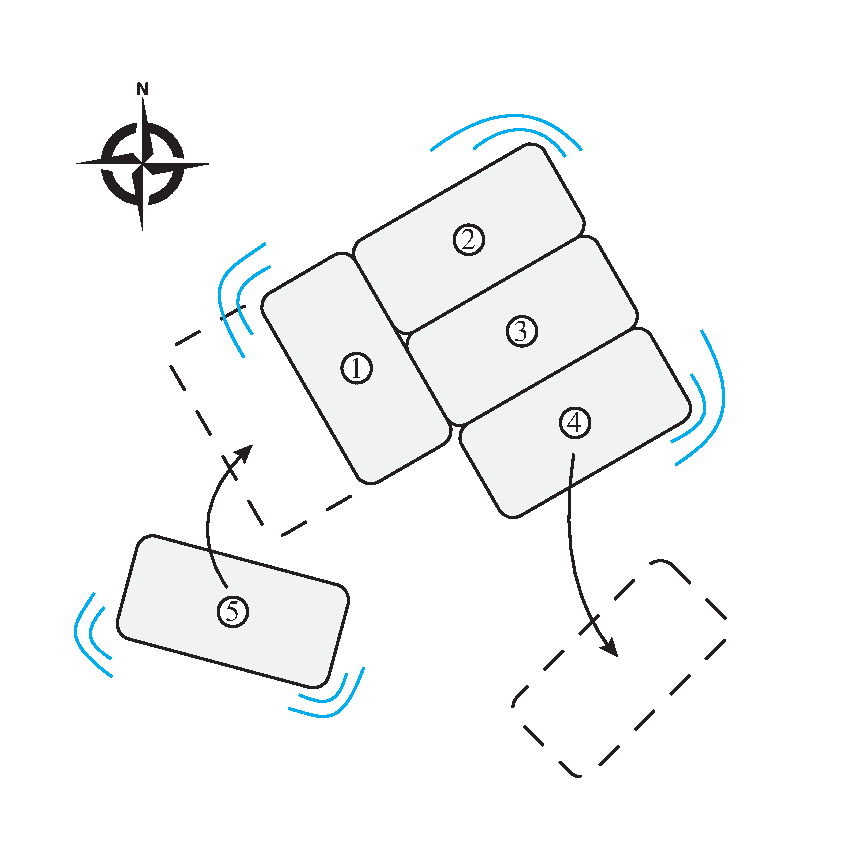
\includegraphics[width=0.95\textwidth]{img/intro_reconfiguration_square}
			\caption{Behavior A: Automatic reconfiguration of a vessel platform. Vessel 1,2,3 \& 4 are connected such that they form a platform. Arrows indicate movement of vessel 5 to connect, and disconnecting of vessel 4.}
			\label{exaA}
		\end{minipage}\hfill
		\begin{minipage}{0.45\textwidth}
			\centering
			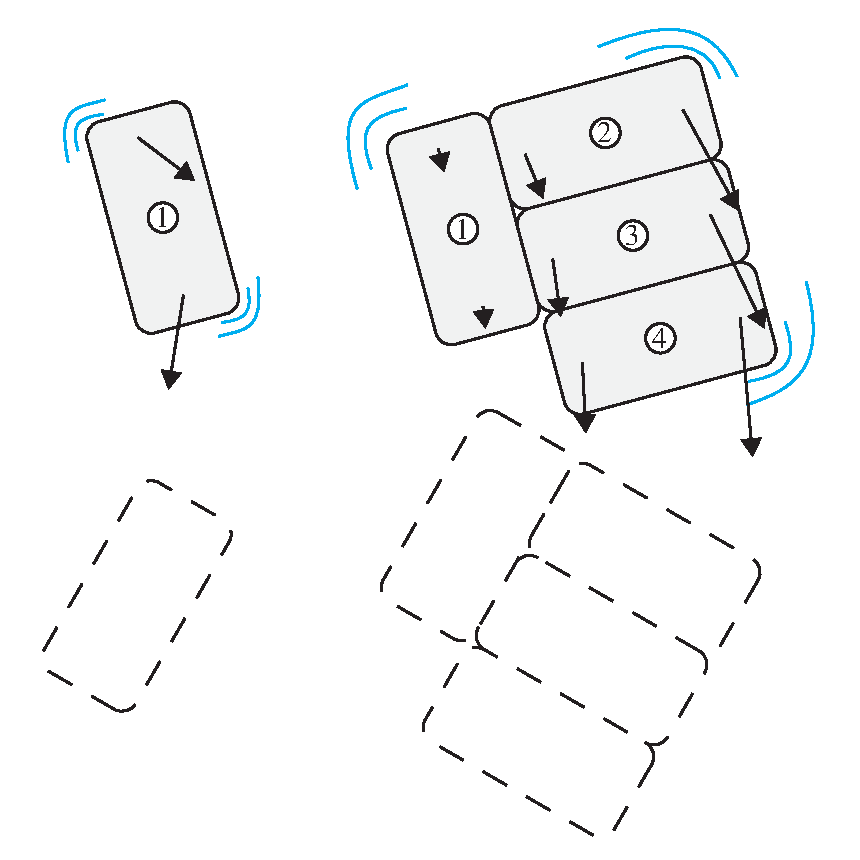
\includegraphics[width=0.95\textwidth]{img/intro_adaptation_square}
			\caption{Behavior B: Fleet control that adapts on platform configuration. The left vessel is configured in the simplest way, and operates alone. Four vessels on the right collaborate to move the connected vessel platform. Arrows illustrate forces generated by thrusters. }
			\label{exaB}
		\end{minipage}
	}
\end{figure}

\section{Problem statement}
It would be useful for developers to know what system requirements, characteristics and constraints emerge from implementing a framework with behavior of system A and B. This information can be used to make well informed, effective, scalable, interoperable and long term beneficial design choices. 

Literature on both systems is available, but there is a lack of content that describes the effect of combining both systems into one, which is the gap of knowledge that this thesis will adress. The research objective of this work is to develop, implement and evaluate a fleet control system performing self assembly and configuration adaptive control within a single framework. 
%The goal of this work is to create a benchmark for automated self-assembling vessel frameworks able to perform platform configuration dependent collaboration.

\section{Approach}
To move torwards realizing implementation of automated vessel platforming systems, this paper strives to fill the gap of knowledge on implementation of automated assembling vessel platforms with configuration adaptive control strategies by seeking to answer the following questions:\\

\noindent {\large\textbf{ Main research question}}
\begin{itemize}
	\item How can a fleet of modular surface platform vessels be controlled to achieve automated assembly and configuration-dependent platform control?
\end{itemize}

 %is split into several subquestions, starting with two regarding previous research and system characterization: 
\noindent {\large\textbf{Sub-questions}}
\begin{enumerate}
\item What is the state of the art within automated vessel platforming systems?
%BEFORE \item \textbf{SQ2} What system characteristics emerge as A and B are integrated?
\item What characteristics does a vessel system have that integrates automated assembly with configuration dependent control?
%\end{enumerate}
%To properly map (possibly unknown) challenges, an experimental setting will be developed that is to show behavior A and B within a single framework. The following subquestions are related to this experimental use case with model scale vessels in lab environment.
\item How can the dynamics of the multi-vessel system be represented?
%\begin{enumerate}
%\item \textbf{SQ3} What are suitable system architectures?
%\item \textbf{SQ4} What are suitable control strategies?
\item How can a fleet control framework be developed that performs automated platform assembly and configuration adaptive platform control? 
\item What is the performance of the developed system?
\end{enumerate}

%\section{Approach}
Subquestion 1 will be answered by means of literature research. This will cover definitions used in the marine control sector, literature related to automated vessel platform assembly systems, and literature related to configuration adaptive platform controllers. The focus is on marine applications, altough general robotic sources are also considered. 

%First, existing literature is explored to answer the first subquestion regarding prior research. A start will be made with exploration of general developments in automated multi-vessel cooperation projects, which will continue to scope down towards papers on automated assembling vessel systems (system A), and configuration adaptive vessel platform control systems (system B). Discussed literature will be mainly regarding marine multi machine cooperation, but projects in aeronautic, automotive or general robotic sectors will be discussed if there are noteworthy similiarities.

Subquestion 2 will be answered by analyzing fundamentals of system A and B. Information from literature on both system A and B will be used with a systematic approach to map and explain fundamental system characteristics (e.g., functions, requirements, limitations, indicators of performance) of A and B. 
Thereafter, predictions will be done how a integration of A and B result in a set of characteristics due to inheritance and interference. Attention is given to scoping down the full range of design choices to a region that is considered to have more potential to be realistically implemented in the near future. 

Subquestion 3 is answered by formulating a multi-vessel state description, formulating a platform-state description and proposing an approach to predict dynamics of a multi-vessel structure from individual module models. 

Subquestion 4 will be answered by developing and implementing a model scale system performing the mentioned behavior. The design is based on formulating a system that is predicted to be most likely implemented in the future from a commercial point of view.  Emphasizing advantages of modular vessel platforms will be prioritized, while some increases of disadvantages are deemed acceptable, as modular vessel structures are expected to be only feasible in scenarios where a specific set of performance indicators are prioritized far above others. 

Subquestion 5 will be answered by evaluating performance of the developed system. This is done according to performance indicators that resulted from answering subquestion 2. Behavior that does not directly impact performance will also be presented if it is relevant to sketch implementational challenges for future marine automation projects. 

Considerations and findings during the whole design process will be documented, to use for future projects, and to formulate into recommendations and discussion on suitable control system designs.

\section{Scope}
The control system for the model scale lab setting will be developed to make a certain configured platform for transporting a large object. For this, three Delfia-1* model vessels (see fig \ref{fig:introDelfias}) from the Reasearchlab Autonomous Shipping (RAS) Delft are used as experimental model scale vessels, which are expected to automatically assemble into a single rigid body and perform several maneuvering tasks in a single assembled configuration. The control system will not be reliant on data from parameter estimation efforts, as this is also not what commercially implemented systems are expected to have. System dynamics are simplified to three degrees of motion in on the surface (x,y, yaw).

This project is limited to finding one solution to the design challenge of the experimental setup. This research will include results gathered during the design process, together with system behavior data of the final framework implemented with the desired behavior A and B. 

All design choices of the final framework will be discussed. Choices of these design choices are affected by the available timeframe, but are required to be able to result into a framework with behavior A and B.

The performance indicators that are deemed most relevant for systems developed in this thesis are: Vessel response, reliability, modularity. Design choices in the implementation of the vessel system will be based on these indicators.  

Assembling systems can work with or without using a target configuration. Self assembly without target configuration can be such as organic growth, or flocking. This paper focusses on systems that generate a target configuration or uses a given desired configuration, that both use a concept of a desired configuration. 

Self-assembly is a form of a more general behavior, self-reconfiguration, which also includes changing of shape and disassembly. This work focusses mainly on the assembly aspect. 

\begin{figure}[h!]
	\centering
	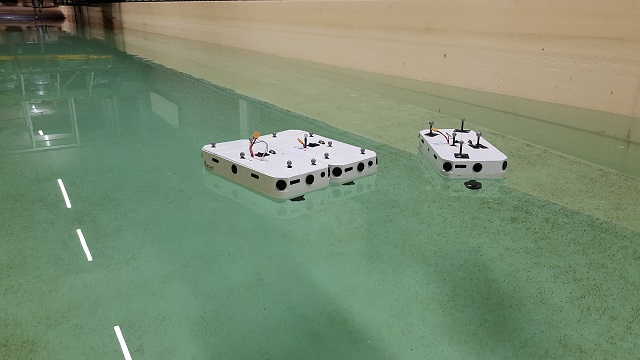
\includegraphics[width=0.6\textwidth]{20210804_171747}
	\caption{Three Delfia-1* modules from RAS Delft in the MTT towing tank facility at 3ME }
	\label{fig:introDelfias}
\end{figure}

\section{Thesis outline}
%This document starts with desribing considerations related to formulating a high level vessel network, it's components. subsystems, agents, and structure. This is followed by a section that focusses on the design choices made on developing the earlier described agents and subsystems. Control strategies in those subsystems will be discussed together with the algorythms that are developed to realize the system behavior. 
The content of this report is as follows:
Chapter 2 answers subquestion 1 by means of literature research on vessel platforming systems and related topics. 
Chapter 3 shows system analysis of behavior A \& B independently, to then predict how functions, requirements, constraints and other characteristics translate and interact in a single system that shows both behaviors which answers subquestion 2.
Chapter 4 describes the proposed multi-vessel and platform state description and a novel approach to predicting dynamics of combined waterborne structures from module models.
Chapter 5 shows the process of designing an implementation of such a system for model scale vessels, to answer subquestion 4. Design choices and considerations are discussed from a high level (a nework) to a low level (behavior of agents within the network) view. 
Chapter 6 aims to analyse performance of the developed framework, by evaluating behavioural responses, thus answering subquestion 5.
Chapter 7 concludes and discusses the findings of this thesis, and finalizes with future recommendations and vision.

Furthermore appendices include (\ref{appendix:techreport})a technical paper that summarizes the work in this project, (\ref{appendix:CombineDynamics}) derivation of the approach to approximate platform dynamics and \ref{appendix:algorythsms} sourcecode of the main algorythms that make up the implemented control software. 

%\begin{table}[h!]
	\centering
	\begin{tabular}{|l|l|l|}
		\hline
		Chapter            & Goal                                                                                                                                              & \begin{tabular}[c]{@{}l@{}}Answers \\ subquestion\end{tabular} \\ \hline
		1: Introduction    & Formulate problem statement, approach, research questions, scope                                                                                  & -                                                              \\ \hline
		2: Prior Works     & \begin{tabular}[c]{@{}l@{}}Summary of works on: automated vessel-platform assembly, \\ platform control\end{tabular}                              & 1                                                              \\ \hline
		3: System Analysis & Map characteristics of self assembly and collaborative platform control.                                                                          & 2                                                              \\ \hline
		4: System Design   & \begin{tabular}[c]{@{}l@{}}Show design process, choices and considerations made to implement\\  a functional vessel system\end{tabular}           & 3                                                              \\ \hline
		5: Evaluation      & \begin{tabular}[c]{@{}l@{}}Evaluate performance of the implemented vessel system in a\\  quantitative manner.\end{tabular}                        & 4                                                              \\ \hline
		6: Conclusion      & \begin{tabular}[c]{@{}l@{}}Conclude by answering the main question. Provide recommendations\\ for future implementation and research\end{tabular} & -                                                              \\ \hline
		Appendix A  & \begin{tabular}[c]{@{}l@{}}Technical paper summarizing the work of this thesis project. \end{tabular} & -                                                              \\ \hline
		Appendix B      & \begin{tabular}[c]{@{}l@{}} An approach to derive  dynamics of combined waterborne structures \end{tabular} & -                                                              \\ \hline
		Appendix C      & \begin{tabular}[c]{@{}l@{}}Sourcecode of the main algorythms that make up the implemented \\ control software.\end{tabular} & -                                                              \\ \hline
		
	\end{tabular}
	\caption{The link between chapters, goals and subquestions. }
	\label{tab:my-table}
\end{table}

	\chapter{Literature survey on modular vessel platform automation}
%{Related work on modular vessel platform automation}
\label{LiteratureStudy}

% Link this chapter in the whole. Whats the role. 
This chapter summarizes literature relevant to automated vessel platforming systems to answer subquestion 1:
\begin{itemize}
	\item What is the state of the art within automated vessel platforming systems?
\end{itemize}

For effective discussion on ship automation good definitions of terminology are required to avoid misinterpretation. Definitions that are used in this work are described in section \ref{literatureDefinitions}, supplemented with various other common interpretations. 

This literature review shows various works on automated control of vessel platforming systems, yet it was noticed that the majority of relevant works focus on either the "assembly process" or "control of a platform with adaptable configuration", so they will be discussed in those groups in section \ref{literatureAutomatedAssemblySystems} and \ref{literatureConfigurationDependentControl} respectively. 

\citet{chen2020survey} provides an overview on cooperative control methods for waterborne transport where  vessel-to-vessel cooperation is classified in three categories; formation control, cooperative collision avoidance, and cooperative manipulation. Vessel platform motion control would fall into the category of cooperative manipulation (a fleet of vessels coordinate their actions to fulfill certain tasks\cite{chen2020survey}). Platform self assembly has facets overlapping with formation control (steering a group of vessels to form a specific geometric configuration and control their coordinated collective motion \cite{chen2020survey}) and cooperative manipulation of the multi-robot fleet. As sources that specifically describe modular vessel platforming systems are limited, so a broader range of works is discussed in this review, such as fields of cooperative manipulation, formation control, and reconfiguration automation from general robotic science. 

Discussed projects are schematically shown in section \ref{literatureConclusion}, where this chapter also elaborates on the resulting gap of knowledge that drives this paper. Various works that are introduced and discussed in this chapter are further used in chapter \ref{chap:sysAnalysis} to analyze system characteristics and discuss design choices and considerations of these projects.

%In the search for literature, the following keywords were used:Autonomy, automated, automation, smart ship, vessel, ship, self-assembly, assembly, platform, platforming

\section{Terminology}
\label{literatureDefinitions}
Definitions used to describe automation of various vessel processes differ a lot troughout the marine sector. Relevant terminology and their interpretation will be discussed here. 

\begin{itemize}
	\item \textbf{Automation} refers to the full or partial replacement of a function previously carried out by the human operator. This implies that automation is not all or none, but can vary across a continuum of levels, from the lowest level of fully manual performance to the highest level of full automation (definition according to \citet{parasuraman2000model}).
	
	\item \textbf{Control} is purposeful action on or in a process to meet specified objectives, which can be exercised by a human or by automation (defnition according to \cite{IMO103ISORegulatoryScopingExMass}). Control, pertaining to a ship, often primarily refers to the motion of the hull, altough other tasks (such as connecting in this paper) can refer to this as well.  
	
	\item \textbf{Modular reconfigurable robot} (MRR) systems are made up of many repeated modules (or units) that can be rearranged or can rearrange themselves into different configurations depending on the task the robot is to solve at the time (definition according to \citet{seo2019modular})
	
	\item \textbf{Configuration} in reconfigurable robotics is commonly generalized to incorporate the connectivity of the modules (which module is connected to which, represented as an adjacency matrix, a linked list, and the like) into the conventional robotics definition of the term that refers to just the pose of the robot (the full set of the joint angles of the	robot) (definition according to \citet{seo2019modular}).
	
	\item \textbf{Reconfiguration} is the process of changing connectivity \citet{seo2019modular}, which may include \textbf{assembly} and/or \textbf{disassembly}.
	
	\item \textbf{Vessel-platform}, or sometimes referred to as platform, is a combination of vessels, or  \textbf{modules} that are connected to form a floating structure.
	
	\item A \textbf{cybernetic} system is self-regulating. The term cybernetics was developed by Norbert Wiener in 1948 \citet{norbert1948or}. This regulation is done by the system according to a given (control) law. \citet {smithers1997autonomy} describes the difference between cybernetics and automation: " Cybernetic systems are thus self-regulating systems, systems that are not just able to move or to act by themselves but are also able to regulate and control their movements or actions so as to maintain their effectiveness in the face of disturbances and perturbations, according to some predefined control law or rule of regulation" 
	
	\item An \textbf{autonomous} system is considered self-governing, thus capable of constructing its own laws, according to \citet{smithers1997autonomy}. In practice the interpretation of "autonomous ship" differs among organisations, generally ranging from being interchangably used with "automated" or "cybernetic".  \citet{smithers1997autonomy} argues that the beforementioned definition is more consistent to use in other sciences while it also functions as an independant important concept; "Autonomous systems are different from cybernetic systems, and they form a more general class of self-regulating systems, those that form their own laws of regulation as well as regulate their behavior with respect to these self-made laws." Indiscriminate use of the term "autonomous" can cause confusion, misinterpretation and false expectations.  For further use in this paper, the term autonomous is avoided as it is deemed too ambiguous at this point and other terminology (cybernetics and automation) suffice.
	
	\item An \textbf{unmanned} surface vessel (USV) is a ship with no humans on board \cite{IMO103ISORegulatoryScopingExMass}. According to this definition being unmanned does not characterize the nature of the controller. The vessel can be controlled by a human, via remote control, or it can be machine controlled to meet its goals. 'Reduction of human presence' and 'reduction of human control' often go hand in hand \cite{heo2017analysis} but are not equal as can be seen from the example of remote-, human-controlled systems. 
	
	\item A ship's \textbf{power source} provides energy to fuel its actuators. There exists a trend in developing electric powered vehicles. Electrification of vehicle's power source is often done with climate influencing emmisions in mind. Vehicle power source, whether fueled by fossil fuels, electric or by other means has no direct influence on the degree of automation. Goals of automation and electrification often overlap, and there are some shared benefits, but they are distinct concepts. 
\end{itemize}

For further reading on definitions, interpretation, categorization and terminology, the following sources are recommended; \citet{vagia2016literature} discusses the evolution of use of 'levels of autonomy' and 'levels of automation' in robotics. It is shown how authors use terminologies and taxonomies in different ways. \citet{smithers1997autonomy}'s describes common use of terms "cybernetics", "automation" and "autonomy", and discusses ways of interpretation. 

The International Maritime Organisation (IMO) shows ongoing changes to the proposed definition of 'autonomy' in the contexts of shipping \citet{IMO103ISORegulatoryScopingExMass} in an effort to standardize usage. The last proposed definition of autonomy appears to mean something different than how it is used in other sciences such as philosophy, biology and psychology. How the marine sector started to adopt the word 'autonomy' and how the use will develop is unclear, but it will need a concrete definition of an overarching organisation such as IMO or ISO to avoid discussion. 

Use of the terminology: "unmanned surface vehicle" (USV) does not always capture the essence of projects that strive towards automation. The term USV could also contain vehicles that are human controlled from a distance by means of remote control. For control purposes it might be more suitable to categorize according to the nature of the controller (human controlled, machine controlled or hybrid), instead of whether there are humans on board or not. 

It is found that when discussing "vessel automation", various topics can stay especially vague. The following questions are considered key to get insights on  a so called 'automated vessel system':
\begin{itemize}
	\item \textbf{What functions are exactly automated?} Generally the main function of a vessel is considered movement, thus the motion control is often seen as the main function. Other tasks such as power management (e.g., fueling), system health monitoring, maintenance or on-board activities could also be implied to  all be automatic on an 'automated ship', although they are often not. Environmental awareness is likely neccesary for vessel automation on busy waterways, as the ship needs to take other entities into account to safely perform its voyage, although not a requirement for basic motion control. 
	\item \textbf{To what degree are these functions automated?} One automated vessel might be to only able to control its position to a reference given by an operator, while more advanced systems equipped with a planning and guidance layer might be able to plan and control a trajectory through dynamic waterways. Various categorizations of automation and autonomy exist, each with their own purpose and complexity, of which many are compared in \citet{vagia2016literature}, for the interested reader.
\end{itemize}

For a history lesson and some fundamentals about vessel control theory, consider reviewing \citet{clarke2003foundations}.
For a regulatory flavour of challenges for vessel automation consider consulting \citet{komianos2018autonomous} as the author examines operational, regulatory and quality assurance challenges due to development and deployment of autonomous vessels. Many projects that work on automated, unmanned or autonomous vessels are summarized, of which most are specifically aiming at deployment at sea. Existing regulations where adaptation is deemed required to allow further ship automation are being discussed. Specific comments about required regulatory changes are discussed on: the Convention of life at sea (SOLAS), the International Convention on Standards of Training, Certification and Watchkeeping for Seafarers (STCW), the Convention on the International Regulations for Preventing Collisions at Sea (COLREG), the International Convention for the Prevention of Pollution from Ships (MARPOL), the International Convention on Maritime Search and Rescue (SAR). Various  interpretations of autonomy and resulting characteristics are quoted, although no single definition is stated. Interpretation ranges from "unmanned" to "machine controlled".

\section{Automated reconfigurating vessel systems}
\label{literatureAutomatedAssemblySystems}

Two projects have been identified to build up the majority of the literature on automation of fleet assembly into floating structures. The first discussed works are on a project that developed a nameless fleet of container-like modules with rope and hook connectors, while the second works are developed in the "Roboat" project with vessels of similar naming. 

%% Container-like fleet
\citet{o2014self} and \citet{paulos2015automated} record developments of their fleet of container-like modules. The vessels are rectangles with dimentions of the same ration of standard shipping containers, but at a model scale (Fig. \ref{fig:o2014selfModuleDesign}). The specific shape is aimed to demonstrate how an upscaled system could be rapidly deployed from standard container carriers. 

% Example bridge
\citet{o2014self} greatly illustrates potential of modular marine structures to solve logistical challenges by forming a bridge that allowed crossing of a remote controlled toy car (figure \ref{fig:o2014selfBridge}). The structure formed consists of partially functioning modules in between. Which functions were active on these modules is not mentioned. It is expected that connection systems were functional on all vessels, while other functions, such as positioning, were active on a part of the fleet. 
 
 \begin{figure}[h!]
	\centering
	\makebox[\textwidth][c]{
		\begin{minipage}{0.45\textwidth}
			\centering
			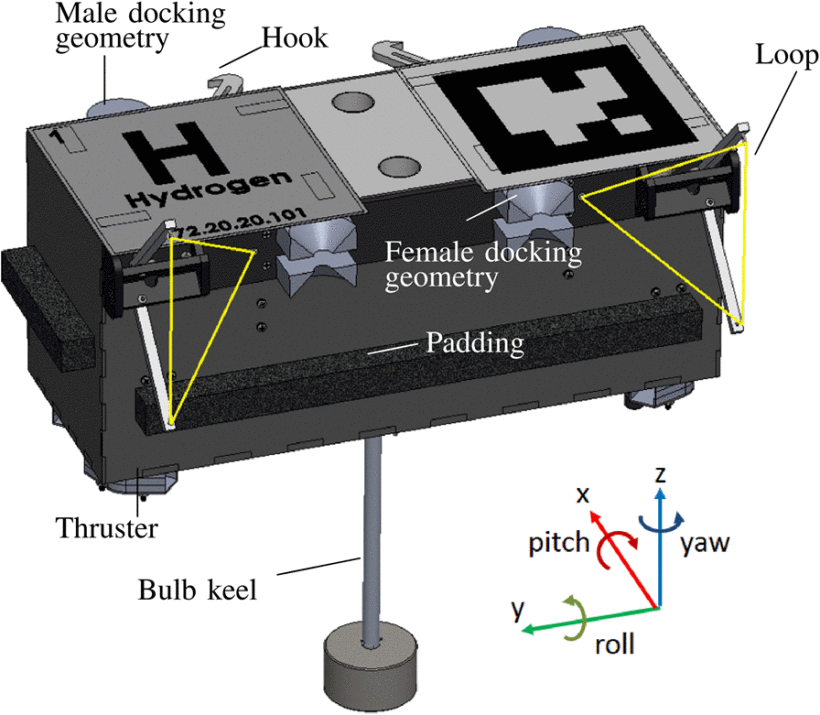
\includegraphics[width=0.95\textwidth]{img/o2014selfModuleDesign}
			\caption{Container-like platform module used in \cite{o2014self} and \cite{paulos2015automated}}
			\label{fig:o2014selfModuleDesign}
		\end{minipage}\hfill
		\begin{minipage}{0.45\textwidth}
			\centering
			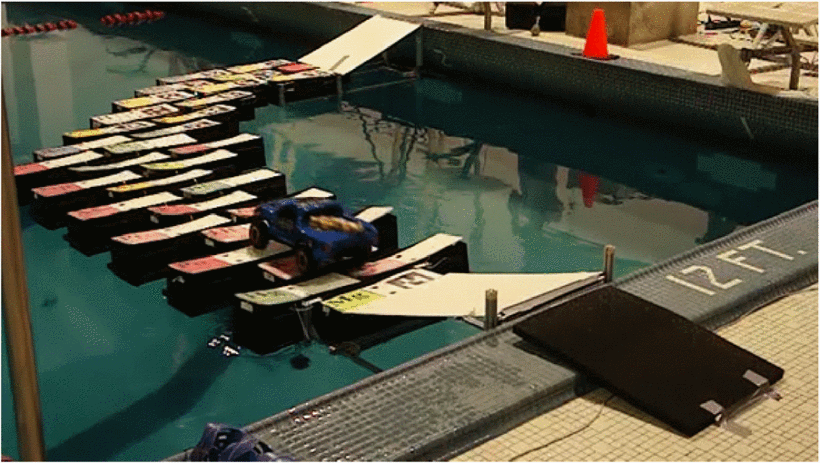
\includegraphics[width=0.95\textwidth]{img/o2014selfBridge}
			\caption{Static floating structure formed from 33 modules \cite{o2014self}}
			\label{fig:o2014selfBridge}
		\end{minipage}
	}
\end{figure}

% Roboat
The Roboat project aims to develop a floating combined infrastructure from modules which are also reffered to as 'Roboats', where the main collaborators are Massachusetts Institute of Technology (MIT) and the Amsterdam institute for Advanced Metropolitan Solutions (AMS). \citet{wang2018design} initially presents the Roboat system equipped with a real-time nonlinear model predictive control system. The vessel design has four thrusters configured in a cross to produce holonomic motions. The design is based to form a framework upon which further tests can be performed for transportation and self-assembly to floating infrastructures. This paper is the first published document on development of the "Roboat" concept, while the project  aims to scale up from model vessels to full scale operation \cite{roboatWebsite}. Early scale up is shown in \citet{wang2020roboat} to a 1.0x2m version at solo operation. All following resources that use Roboat equipment are however based on the smaller models. 

\begin{figure}[h!]
	\centering
	\makebox[\textwidth][c]{
		\begin{minipage}{0.45\textwidth}
			\centering
			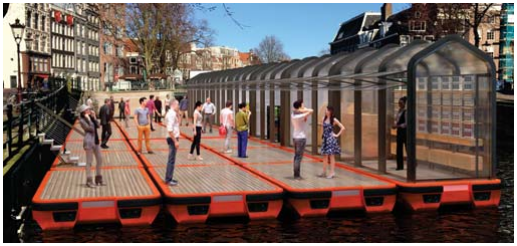
\includegraphics[width=0.95\textwidth]{img/roboatStructureConcept}
			\caption{Roboat's concept of creating floating structures from square modules \citet{wang2018design}.}
			\label{roboatStructureConcept}
		\end{minipage}\hfill
		\begin{minipage}{0.45\textwidth}
			\centering
			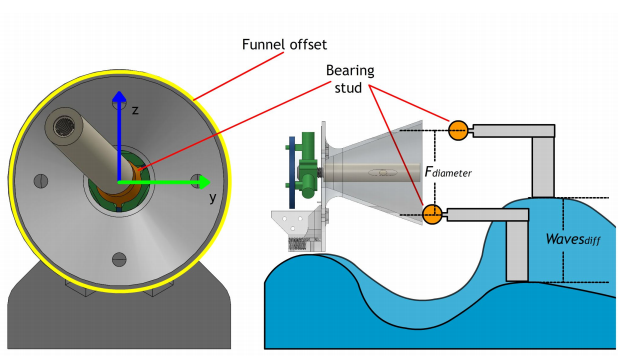
\includegraphics[width=0.95\textwidth]{img/roboatLatchingBallcone}
			\caption{ \citet{mateos2019autonomous} shows a ball and funnel connection mechanism tested on Roboat vessels.}
			\label{roboatLatchingBallcone}
		\end{minipage}
	}
\end{figure}

\citet{mateos2019autonomous} shows development of a latching system consisting of male/female ball/cone components. This paper discusses latching hardware and shows experimental results of a vessel system that performs platform assembly with the implemented latching hardware.

\citet{8901099} and \citet{kelly2019algorithms} present trajectory planning algorythms for reconfiguration of modular surface structure components. The proposed core logic of the shapeshifting algorythm is in finding the largest overlap between current and desired configuration. Overall phases of the proposed reconfiguration scheduler are shown in figure \ref{fig:kelly2019algorithms_statemachine_schematic}. \citet{8901099} show approaches and experimental results of platform shapeshifting, by distincting the whole reconfiguration problem into task planning, trajectory planning and trajectory tracking (see Fig. \ref{fig:roboatreconfigurationplanning}). 

\begin{figure}[H]
	\centering
	\makebox[\textwidth][c]{
		\begin{minipage}{0.45\textwidth}
			\centering
			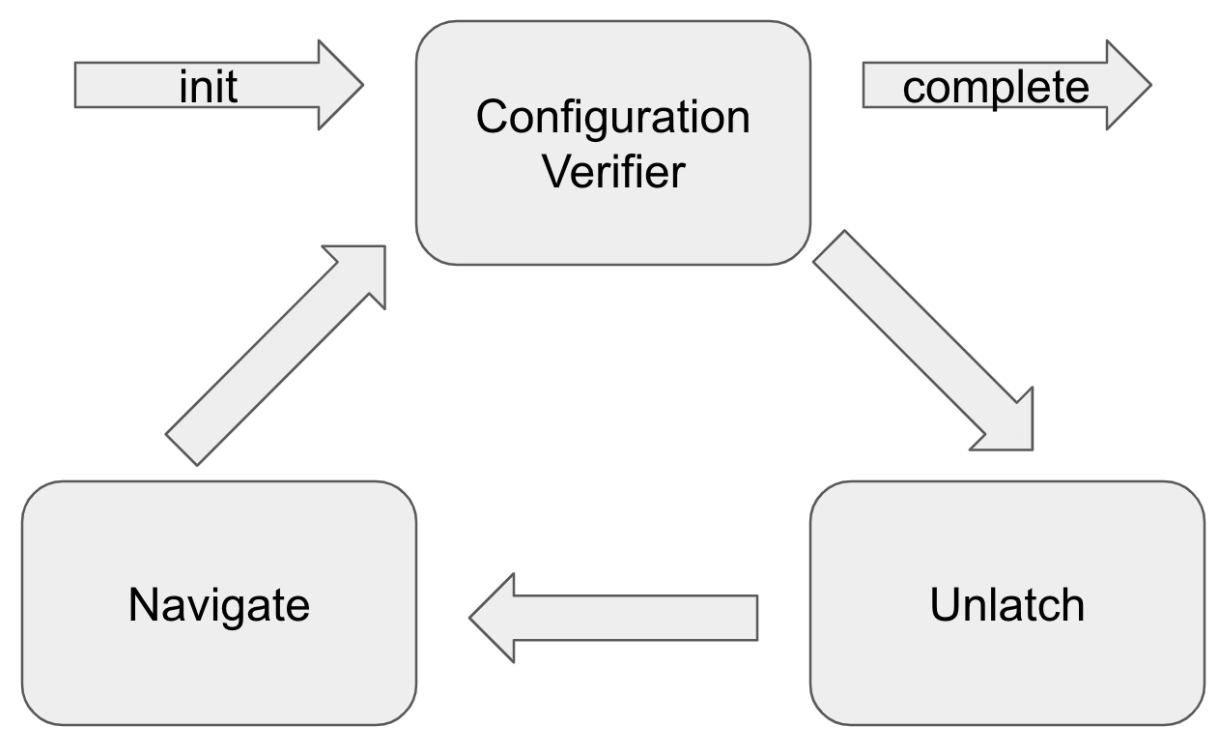
\includegraphics[width=0.95\textwidth]{img/kelly2019algorithms_statemachine_schematic}
			\caption{Platform reconfiguration system phases from \citet{kelly2019algorithms}}
			\label{fig:kelly2019algorithms_statemachine_schematic}
		\end{minipage}\hfill
		\begin{minipage}{0.45\textwidth}
			\centering
			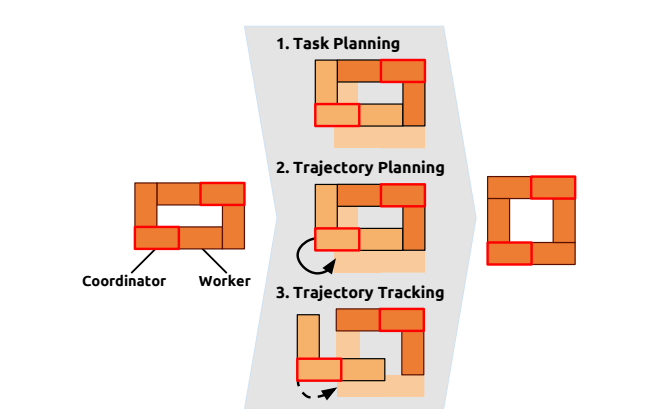
\includegraphics[width=0.95\textwidth]{img/RoboatReconfigurationPlanning}
			\caption{Shapeshifting process of \citet{8901099} in Three Stages: 1) Task Planning finds
				a decomposition for unlatching into two assemblies and relatching
				them in a desired shape. 2) Trajectory Planning computes a
				trajectory for one assembly from one latching point to another one.
				3) Trajectory Tracking controls the assembly along the trajectory. }
			\label{fig:roboatreconfigurationplanning}
		\end{minipage}
	}
\end{figure}

The literature on non-maritime multi robot assembly proved to be more expansive, thus readers are encouraged to take a further look at this if they are interested to get inspired from a broader body of literature. Two of such works on assembly of general robotic systems are as follows.

\citet{tuci2018cooperative} describes key literature on assembly of multi-robot systems. The author noticed the pattern in studies that gave reason to distinct three physical connection strategies in multi-agent systems: Pushing only, grasping, and caging. This reseach had no focus on vessels or orher marine applications, but describes many great works from a broader, general robotics body of literature. 

\citet{miyashita2008morphology} shows the relation between morphology on the success of assembly in the eventually desired shape of stochastic robots. This work took inspiration from biological examples of self-assembly to design and build a water-based modular robotic system consisting of plastic tiles capable of aggregation on the water surface. An externally applied electric potential controlled the self-assembly of the aggregates. This paper is particularly interesting as it shows a completely different approach (stochastic vs deterministic) and operational scale than the container like modules and the Roboat project, illustrating the vast amount of possible solutions to self-assembly challenges. 

\section{Collaborative motion control}
\label{literatureConfigurationDependentControl}

As arbitrary shaped waterborne structures are formed, it can be beneficial to be able to manipulate motion of the combined body. This section discusses works that focus on cooperative manipulation of waterborne objects. Modular strucures are of particular interest, although works describing motion control of such systems are limited. The majority of the encountered literature focusses on controlling motion of a single large object  (e.g. a large unactuated barge) by utilizing combined effort of  a fleet of automated vessels (e.g. tugboats). 

\citet{johansen2013control} distincts three levels of hierarchy for motion control of over-actuated systems, as shown in Fig. \ref{johansen2013controlDistinction}. A high level motion control system generates virtual control efforts to meet control objectives. A second system allocates the desired virtual control effort between actuators, possibly taking into account issues such as actuator saturation and meeting secondary objectives such as power efficiency optimization. A third layer operates on the level of a single actuator such that it meets allocated state (e.g. propeller speed, actuator orientation). \citet{johansen2013control} provides a varied survey on control allocation algorithms from aerospace, maritime, automotive and mechatronic industries. Algorithms are classified in two main classes based on using linear or nonlinear models. 
	\begin{figure}[h]
		\centering
		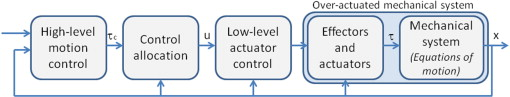
\includegraphics[width=0.7\textwidth]{ControlAllocationLoopExplained}
		\caption{\citet{johansen2013control} Control system structure including control allocation. The vector  denotes commanded virtual control effort (generalized forces), while  are the actual allocated control effort.}
		\label{johansen2013controlDistinction}
	\end{figure}
\citet{johansen2013control} mentions that the design on the control allocation algorithm and the high-level motion control algorithm cannot always be independent, and lack of feasibility of the control allocation should be observed and handled by the high-level motion control algorithm in order to avoid unacceptable degradation of performance in such cases. This division of the control system generally pertains a more common single vessel scenario, yet these principles are applied throughout the majority of multi-vessel scenarios as well. 

Various works describe different approaches for controlling motion of a larger vessel using a fleet of smaller modules (see 
\citet{feemster2006manipulation},\citet{4282954},  \cite{feemster2011comprehensive},  \citet{smith2007swarn}, \citet{bidikli2016robust}, \citet{esposito2008cooperative}, \citet{du2020cooperative},    
 and more). A generic usecase is motion of an uncontrolled ship with a fleet of small tugboats, as shown in Fig \ref{feemster2006manipulationExample}.  These works bear significant similarities with motion control of a modular platform, as both challenges are a form of collaborative manipulation. However, they differ as these works assume constant shape and dynamics of the controlled vessel. This often allows to reasonably assume that ship dynamics are known, which cannot easily be said for modular structures. A selection of these works that were found to illustrate a specific challenge or approach are briefly discussed. 
	
\begin{figure}[h!]
	\centering
	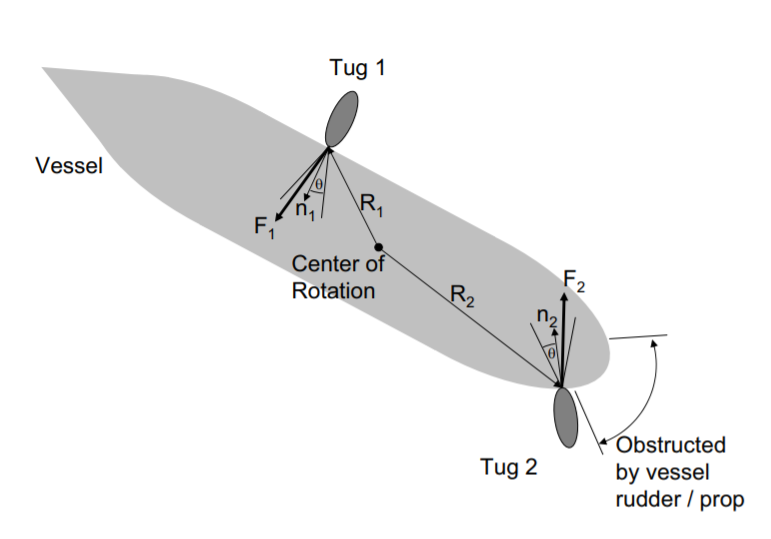
\includegraphics[width=0.5\textwidth]{feemster2006CollaborativeTugboat}
	\caption{Illustration of swarm forces on disabled vessel (\citet{feemster2006manipulation})}
	\label{feemster2006manipulationExample}
\end{figure}

\citet{feemster2006manipulation} considers the control problem of cooperative manipulation of a larger object by a team of smaller robotic vessels using a decentralized architecture. This work focusses on controlling only rotation, yet shows approaches and considerations to avoid a single point of failure from a centralized architecture. Other works also explore distributed control approaches, such as \citet{4282954},\citet{habibi2016distributed} and \citet{chen2019distributed}.

\citet{feemster2011comprehensive} presents a trajectory tracking framework of cooperative ship manipulation. Primary challenges are identified and described as: (1) the actuators are unidirectional and experience saturation; (2) the hydrodynamics of the system are difficult to characterize; and (3) obtaining acceptable performance under field conditions. An experimental setup shows a proposed control approach with separate trajectory generation, tracking control, and force allocation taking into account saturation of actuators. The controller employs an adaptive feedback law to compensate for unknown—difficult to measure—hydrodynamic parameters, employing a 3-DOF planar second order dynamical model. 

Various connection mechanisms are described in existing literature, each with different characteristics. \citet{smith2007swarn} investigates utilization of a swarm of automated tug boats to manipulate an object, where the tugboats are constrained to only exert a pushing force.  \citet{chen2019distributed} sheds light on contact dynamics in a cooperative manipulation challenge where tugboats can only exert pulling force, while also taking into account connector dynamics of an elastic towing line. 

\citet{bidikli2016robust} proposes an approach to control a large object with pushing tugboats, while his framework supports changing configuration as a novelty. The tugboats exert forces on the barge, and are treated as actuators of the large ship with time varying thruster-configuration. The controlled object is assumed under influence of hydrodynamic mass effects  and a self-tuning control gain strategy is employed. Efficiency of the presented controller is demonstrated trough simulation.

\citet{du2020cooperative} describes such a multi-vessel control architecture where tugboats are designed to satisfy allocated towing forces and angles. This formalized layers illustrate how tugboats effectively function as acuators with their own specific dynamics. This work is extended in \citet{du2021cooperative} to incorporate environmental disturbances. 

Contrary to previously mentioned works, \citet{park2019coordinated}  describes an approach of controlling a modular structure. The vessels that combine into the combined body are by themselves already fully actuated. The main control approach used is a PD controller to generate control effort, which is said be applicable to any configuration and reference. Allocating control effort between thrusters is implemented as an optimizer minimizing energy use to find actuator response. Experimental results show effectiveness of the proposed control strategy on three different configurations. 
The control system design is based on an approximate model, which scales according to a variable amount of vessels that are coneccted into the platform, but not to configuration shape. Translational inertia (directional dependent masses in x and y direction) is assumed to scale with $n$ amount of vessels, while rotational inertia was scaled quadratic by $n^2$. System inertia is represented by constant directional dependent mass as the sum of rigid body and hydrodynamic-added mass. 

\begin{figure}[h!]
	\centering
	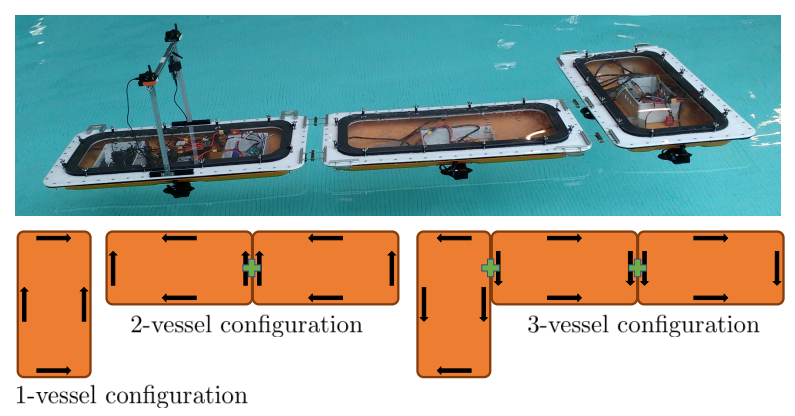
\includegraphics[width=0.6\textwidth]{park2019coordinatedConfigurations}
	\caption{ (Top) L-shape configuration of the connected-vessel platform and
		(Bottom) 3 different configurations used in the experiments. \citet{park2019coordinated}}
	\label{fig:park2019coordinatedConfigurations}
\end{figure}


\begin{figure}[h!]
	\centering
	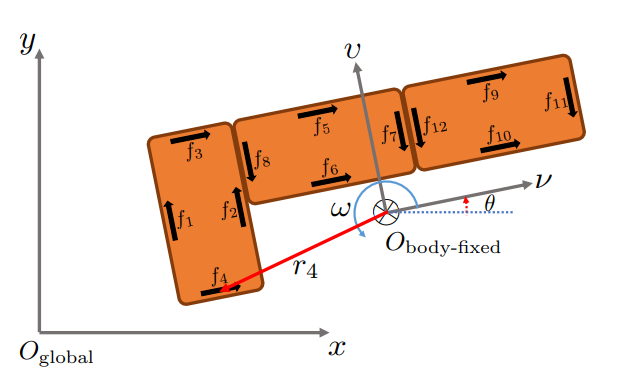
\includegraphics[width=0.5\textwidth]{park2019coordinatedBodyFrame2}
	\caption{An example of a rigid body of three connected vessels, where each black arrow drawn on the body of a vessel represents force exerted from a propeller. \citet{park2019coordinated}}
	\label{fig:park2019coordinatedBodyFrame}
\end{figure}

Scenarios where smaller vessels manipulate a significantly larger object, dynamics of the manipulators might be neglectible. However, assemblies with comparably sized modules will have rigid body dynamics affected by the configuration. \citet{park2019coordinated} distinguishes itself from the previously mentioned works as it attempts to predict dynamics of the assembly based on the configuration, albeit only on numbers and not on shape. \citet{park2019coordinated} proposes scaling rules to formulate the approximate platform model, as this is a key challenge that needs to be faced for model based controllers for modular strucures. 

\section{Gap in knowledge}
\label{literatureConclusion}
Works on modular vessel platform automation found through this literature survey originated from two project concepts; container shaped modules \cite{o2014self} shown in Fig \ref{fig:o2014selfModuleDesign} and Roboat \citet{wang2018design} shown in Fig \ref{roboatStructureConcept}). Contributions using Roboat vessels are credited to Advanced Metropolitan Solutions (AMS), Massachusetts Institute of Technology (MIT) or their collaboration. More literature exists on concepts that share similarities with vessel platform automation, but miss characteristics to classify as such. The majority of this relevant literature describe approaches for controlling a non-modular object using a fleet of smaller automated vessels. 

The discussed projects have a variety of works that explore facets on vessel platform automation, also showing many different design choices and approaches. Projects regarding automation of a multi-robot system performing reconfiguration or configuration dependent control are shown in table \ref{table:bigbadLiteratureSummary} to aid comparison. Works on multi-robot assembly and collaboration from aerospace and automotive branches have also been included in this schematic to give some perspective on developments in other fields. 

From this literature research it was concluded that no information is found of an modular fleet system that incorporates automated reconfiguration with collaborative configuration dependent control strategies in a single framework. Table \ref{table:bigbadLiteratureSummary} shows that works focus on either reconfiguration or collaborative control, not on combining the two, thus consequences of integrating the two behaviors in a single system are unmapped. Gathering and documenting approaches and experiences on integration can pave the road towards effective implementations to fully benefit from automated structure assembly while motion control of the combined platforms are enhanced by effective collaborative approaches. 

\newpage
\begin{sidewaystable}

\footnotesize
\begin{tabular}{|l|l|l|l|l|l|l|l|l|}
	\hline	
	\textbf{Title} & \textbf{Author} & \textbf{Year} &\makecell{\textbf{Land,} \\ \textbf{naval or} \\ \textbf{aerial}} &  \makecell{\textbf{Simulation or} \\ \textbf{experimental}} & \makecell{\textbf{Automated} \\ \textbf{assembly}}  & \makecell{\textbf{Changing control} \\  \textbf{system during} \\ \textbf{operation}} & \makecell{\textbf{System is} \\ \textbf{config.} \\ \textbf{dependent}} & \makecell{\textbf{Controlled} \\ \textbf{object is} \\ \textbf{modular}}  \\ \hline	
		
	\makecell{Autonomous self-assembly\\  in swarm-bots} & \citet{gross2006autonomous} 	& 2006 	& Land     	& Both  	& Yes  	& No		& No & Yes	\\ \hline
	\makecell{Object transport by modular \\ robots that self-assemble}& \citet{gross2006object}& 2006& Land & Experiment & Yes  & Yes	& No   & Yes  \\ \hline
	\makecell{A novel autonomous self-assembly \\ distributed swarm flying robot}& \citet{wei2013novel}& 2013& Aerial + land & Both& Yes& Yes& Yes &Yes\\ \hline
	\makecell{Self-assembly of a swarm of \\ autonomous boats into floating \\ structures}					& \citet{o2014self}        			& 2014     	& Naval                     	& Experiment             	& Yes                  & No         				& No      &Yes		\\ \hline
	\makecell{Automated Self-Assembly of Large \\  Maritime Structures by a Team of \\ Robotic Boats}		& \citet{paulos2015automated}        	& 2015     	& Naval                     	& Experiment             	& Yes                  & No         				& No      &Yes		\\ \hline
	\makecell{Cooperative Multi-Vessel Systems \\ for Waterborne Transport}                        				& \citet{chen2019cooperative}        	& 2019          & Naval                     	& Simulation                &  No               	& No         				& No   	&No	\\ \hline
	\makecell{Coordinated Control of a Reconfigurable \\ Multi-Vessel Platform: Robust Control \\Approach}     	& \citet{park2019coordinated}        	& 2019    	& Naval                  	& Both       			&  No                	& No                        		& Yes         &Yes 	\\ \hline
	\makecell{Autonomous latching system for \\robotic boats}     										& \citet{mateos2019autonomous}       & 2019    	& Naval                  	& Experiment			&  Yes                	& No                        		& No        &Yes  	\\ \hline
	\makecell{Trajectory Planning for the  \\ Shapeshifting of Autonomous Surface Vessels}     										& \citet{8901099}       & 2019    	& Naval                  	& Experiment			&  Yes                	& No                        		& No     &Yes     	\\ \hline
	\makecell{Algorithms for planning and \\ executing multi-roboat shapeshifting}     										& \citet{kelly2019algorithms}       & 2019    	& Naval                  	& Experiment			&  Yes                	& No                        		& No       &Yes  	\\ \hline
	\makecell{	Manipulation of large objects by swarms\\
		 		of autonomous marine vehicles. Part \\ 
		 		1-Rotation} 	& \citet{feemster2006manipulation}       & 2006    	& Naval                  	& Neither			&  Noy 	&  No 	&  Yes  & No \\ \hline
	\makecell{Positioning of Large Surface \\ Vessels using Multiple Tugboats} 	& \citet{4282954}       & 2007    	& Naval  	& Simulation		&   No  	& No 	&  Yes & No \\ \hline
	\makecell{Comprehensive framework for tracking control\\ and thrust allocation for a highly overactuated \\ autonomous surface vessel} 	& \citet{feemster2011comprehensive}       & 2011    	& Naval 	& Experiment		&  No 	& No	& Yes & No \\ \hline
	\makecell{Swarn Manipulation Of An Unactuated \\ Surface Vessel} 	& \citet{smith2007swarn}       & 2007    	& Naval & Simulation			&  No 	& No & Yes & No \\ \hline
	\makecell{Robust dynamic positioning of surface \\ vessels via multiple unidirectional \\ tugboats} 	& \citet{bidikli2016robust}   & 2016& Naval& Simulation	&  No 	& No & Yes & No \\ \hline
	\makecell{Cooperative manipulation on the water \\ using a swarm of autonomous tugboats} 	& \citet{esposito2008cooperative}& 2008& Naval & Experiment&  No &  No & Yes & No \\ \hline
	\makecell{Distributed model predictive control for\\ cooperative floating object transport \\ with multi-vessel systems} & \citet{chen2019distributed}& 2019 & Naval& Simulation	& No & No& Yes & No  \\ \hline
	\makecell{Cooperative control of autonomous tugs \\ for ship towing} 	& \citet{du2020cooperative}& 2020& Naval&Simulation& No& No & Yes& No \\ \hline 
\end{tabular}
\caption{Comparison of various projects related to vessel platform self assembly and/or collaborative platform motion control}
\label{table:bigbadLiteratureSummary}
\end{sidewaystable}

\newpage



	\chapter{System Analysis}
\label{chap:sysAnalysis}

% Goal of chapter:
This chapter formulates characteristics of the two considered systems and their combination, to answer subquestion 2:

\begin{itemize}
\item What characteristics does a vessel system have that integrates automated assembly with configuration dependent control?
\end{itemize}

Answering this question will bring better understanding of the meaning of "a system that performs self-assembly" and "a multi-robot-assembly performing collaborative and coordinated control". The aim is to look beyond the design solutions from the projects described in the previous secion, and create a broader view on the design spectrum. 

% Structure of chapter
The first section explores characteristics of systems performing automated assembly (section \ref{analysisReconfiguration}) and configuration dependent control (section \ref{analysisConfigAdaptation}).
This chapter concludes by mapping system characteristics as a result of integrating both behaviors (section \ref{analysisCombined}). 

This section uses various external sources to aid formulation of characteristics, some of which have been discussed in the previous chapter. 
The overall approach is to distinct generalized system characteristics as well as a narrowed down set of solutions that can be considered more feasible to perform in commercial applications, also taking into account design choices of other projects. 


\section{Analysis of first required behavior: Automatic vessel platform reconfiguration}
\label{analysisReconfiguration}

Automated modular vessel platform reconfiguration systems can be categorized as a more general "modular reconfigurable robot" system. 
Modular reconfigurable vessel systems can be evaluated from a non-maritime perspective, so where we are not directly focussing on vessels, but on more general modular reconfigurable robot (MRR) systems. \citet{seo2019modular} describes an MRR system as made up of many repeated modules (or units) that can be rearranged- or can rearrange themselves into different configurations depending on the task the robot is to solve at the time. The key characteristic of such systems is described as adaptability of hardware structure to suit a given task or environment. MRR systems differentiate themselves from normal robot systems by determining and executing a course of action, to change it's configuration. 

Various requirements of floating MRR systems were identified during the course of the project. Some approaches originating from sources about robotics in general were broader than approaches encountered in sources about modular vessel platforming. This section aims to conclude with two things. Firstly, it searches for fundamental characteristics of an automatic reconfiguring vessel platforming system. Secondly, the whole range of design choices and approaches is scoped down to a set that is expected to have the highest commercial feasibility. This is based on design choices of prior projects, supplemented with the authors argumented vision. 
During elaboration on system characteristics, prior projects will be discussed, more specifically, how they solved their challenges and in which characteristics did this result in. Automated vessel platform reconfiguration characteristics are discussed in 2 aspects; Strategies and Actuation. 



\subsection{Strategies}
\citet{yim2007modular} describes a taxonomy of architectures of modular robots, which is adopted to the use case of surface vessel platform reconfiguration. MRR system architectures are classified in three generally observed classes. They are described as follows \cite{yim2007modular}
\begin{itemize}
	\item \textbf{Lattice Reconfiguration Architectures} have units that are arranged and connected in some regular, three-dimensional pattern, resulting in a relatively simple and easily scalabe system. 
	\item \textbf{Chain or Tree Architectures} have	units that are connected together in a string or tree topology. This chain or tree can fold up to become space filling, but the underlying architecture is serial.
	\item \textbf{Mobile Architectures} have units that use the environment to maneuver around and can either hook up to form complex chains or lattices or form a number of smaller robots that execute coordinated movements and together form a larger	“virtual” network. 
\end{itemize}

We can see that \citet{o2014self} uses a lattice reconfiguration architecture in the horizontal surface plane (figure \ref{fig:wuh_assembly_planning}). Roboat shows L configurations in various publications, which can be considered a chain architecture, as configurations are used that do not fit in a repeating (lattice) pattern. Roboat reduces the amount of possible configurations by utilizing the square shape of the vessels to reduce the amount of orientations to steps in relative angle of 90 degrees.

Another classification can be found in the way structures are (re)configured. \citet{yim2007modular} distincts two approaches:
\begin{itemize}
	\item \textbf{Deterministic Reconfiguration} uses modules that are purposely manipulated to a target location.
	\item \textbf{Stochastic Reconfiguration} relies on statistics of a set of modules to configure in a more desirable configuration. System design is aimed to reach acceptable configuration without the need of predefined reconfiguration planning.
\end{itemize}

Stochastic reconfiguration can be achieved with very limited functionality per module. Due to robot simplicity, this approach can very desirable on micro scale which can be scaled to great numbers.
Deterministic reconfiguration needs more functionality embedded in a module. This system requires an agent that makes some form of plan, which is then to be executed. As a plan is formed and executed, this approach does give the opportunity to give more guarantees that a desired configuration is reached within a timespan. 

Due to technological advances, communication and computational hardware has become increasingly affordable. If the amount of modules in a system is relatively small, then equipping each individual with communication, computation and control systems is feasible. This allows creation of networks of robots that can share information, collaborate, negotiate and utilize benefits of all sorts of layered control architectures. Both \citet{o2014self} and Roboat utilize a deterministic approach to reach assembly. 

A common approach to solving the task of deterministic reconfiguration is dividing it in several tasks. \citet{o2014self} describes the following states to reach assembly:

\begin{itemize}
	\item Generation of desired configuration. \citet{o2014self} describes the result as a blueprint with a map of relative boat positions. 
	\item Connecting sequence selection. An entity selects a sequence in which the assembly is to happen. 
	\item Positioning of a module.  A trajectory of a vessel to an assembly location is generated and realized by actuators. 
	\item Docking Sequence. As a vessel reaches a docking site within an area of acceptance, the docking sequence runs, which should finalize the docking of that vessel. 
\end{itemize}

\citet{o2014self} greatly illustrates how they formulated strategies for generating connection sequence and module positioning (figure \ref{fig:wuh_assembly_planning} and \ref{fig:wuh_assem_approach})
 \begin{figure}[h!]
	\centering
	\makebox[\textwidth][c]{
		\begin{minipage}{0.45\textwidth}
			\centering
			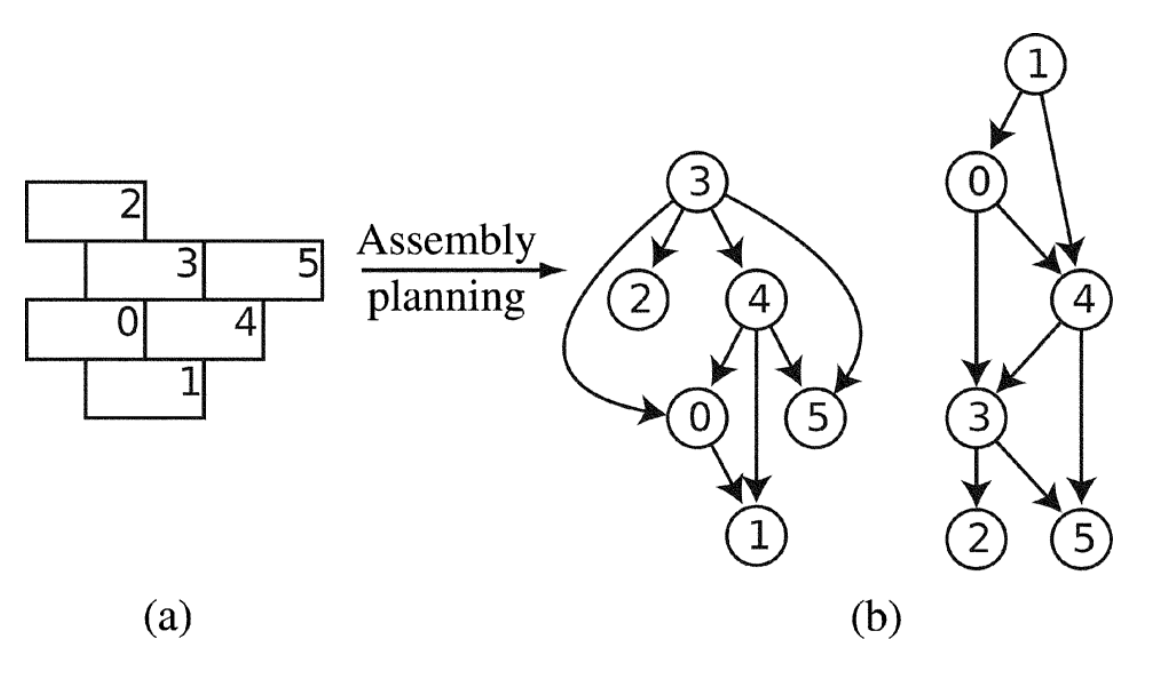
\includegraphics[width=0.95\textwidth]{img/wuh_assembly_planning}
			\caption{The assembly planning stage of \citet{o2014self}, showing desired platform blueprint (a) and two cannidate assembly sequences (b).}
			\label{fig:wuh_assembly_planning}
		\end{minipage}\hfill
		\begin{minipage}{0.45\textwidth}
			\centering
			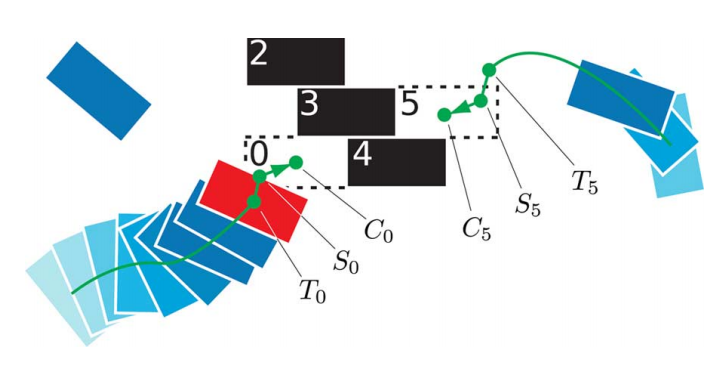
\includegraphics[width=0.95\textwidth]{img/wuh_assem_approach}
			\caption{The trajectory of assembling modules positioning to continue into a docking sequence \cite{o2014self}.}
			\label{fig:wuh_assem_approach}
		\end{minipage}
	}
\end{figure}

\subsection{Actuation}
Two tasks are identified that must be realized by actuators of the system:
\begin{itemize}
	\item means of relative repositioning modules during reconfiguration
	\item means of maintaining acceptable relative position between modules when connected
\end{itemize}

Altough these tasks can theoretically be done by a single system, \citet{seo2019modular} notices that MRR modules generally have two actuator systems to adress these tasks; a large main actuator to move itself with respect to other modules, and a smaller actuator that connects or disconnect two modules. 

The main actuator of MRR systems can be measured in nondimensional characteristic length, being "the number of modules that can be supported in a cantilever fashion under gravity"\cite{seo2019modular}. This measure is perhaps useful for some robotic systems, but does not make sense to use for vessel platforming systems, as gravitation is cancelled out by buoyancy and hydrodynamic forces. These forces are defined as \citet{fossen2011handbook}:
\begin{itemize}
	\item Buoyancy force due to the hydrostatic pressure (proportional to the displacement of the ship).
	\item Hydrodynamic force due to the hydrodynamic pressure (approximately proportional to the square of
	the relative speed to the water).
\end{itemize}

Vessel platforms are not considered excelling at tasks that require large speeds, but rather tasks that benefit from versatility, robustness  and low cost\cite{seo2019modular}. Vessels platforms with relatively low operational speeds can be classified as "Displacement Vessels" \citet{faltinsen2005hydrodynamics}
\begin{equation}
	Fn =  \frac{U}{\sqrt{gL}} < 0.4 \mbox{ }\mbox{ }\mbox{ }\mbox{ for vessels categorized as "Displacement Vessels"}
\end{equation} 

The nature of displacement vessels allow horizontal movement of masses (the ship itself and cargo) much higher with respect to robotic systems that lift, which results in a completely different order of magnitude of the ratio between propulsion and inertia. 
Vessel modules do need means of relocation with respect to other vessels with enough strength to overcome reasonable disturbances, such as wind or current. Further increasing the magnitude of forces that relocate the module reduces the achievable time that a module needs to relocate, which is also dependent on inertia and drag. Strength of main actuator and module mass are affected by various design choices, but optimal choices vary widely per use case. 
Systems that fulfull the task of moving the vessel in the surface plane come in many forms and configurations. Common actuators are propellers, rudders or fins. It is often considered desirable to have a set of actuators that allow imposing forces on all the three degrees of freedom independently, such that we can consider the module fully actuated. Figure \ref{fig:roboatAllocation} and \ref{fig:modularContainerAssembly} show actuator setups of the Roboat and \citet{o2014self}, which can both be considered fully actuated. 

 \begin{figure}[h!]
	\centering
	\makebox[\textwidth][c]{
		\begin{minipage}{0.45\textwidth}
			\centering
			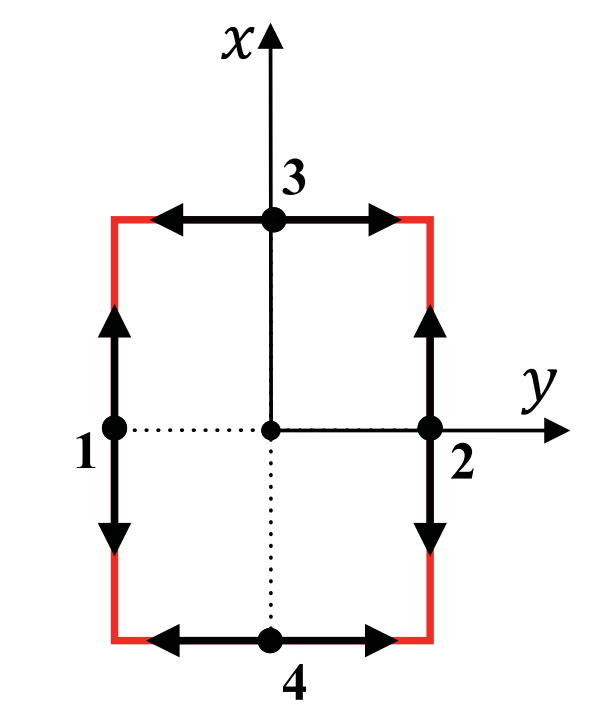
\includegraphics[width=0.75\textwidth]{img/roboatThrusterAllocationPlus}
			\caption{The "+" shaped thruster setup of Roboat \cite{wang2018design}}
			\label{fig:roboatAllocation}
		\end{minipage}\hfill
		\begin{minipage}{0.45\textwidth}
			\centering
			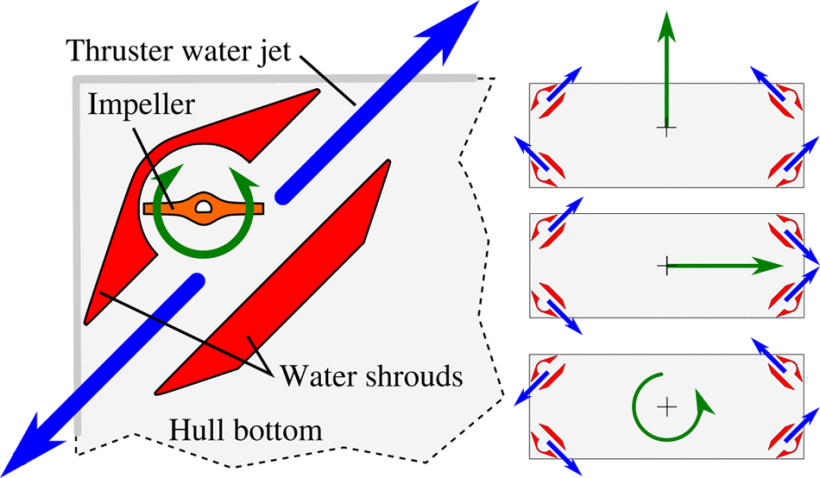
\includegraphics[width=0.9\textwidth]{img/TEMPMThrusterAllocation}
			\caption{The "x" shaped hruster setup of "Tactically expandable maritime platform module" \cite{o2014self}}
			\label{fig:modularContainerAssembly}
		\end{minipage}
	}
\end{figure}

A vessel platforming system needs means to maintain its configuration, which can be achieved using physical restraints that limit relative motion between modules for some period of operation. Movement of the platform as a whole can be desired, for instance when a vessel platform is performing a task of moving to a certain point or orientation. Undesired movement can be caused by disturbances. Alhough maintaining configuration of a vessel platform can theoretically be realized by the main actuators of the module, it is often seen that a second type of actuator is applied, specifically designed to reduce unwanted relative motion between modules by means of physical constraint. Generally once such systems are implemented, often by  mechanical \cite{mateos2019autonomous} \cite{o2014self} or magnetic \cite{kelly2019algorithms} means, the configuration is considered an assembly.


The application of MRR systems on vessel platforms is a niche which generally has specific goals, constraints, environments. The majority of the motion is on the surface plane, often allowing engineers to consider only three degrees of freedom. The environment already enforces some degree of dampening to the system, as various hydrodynamic dampening effects are always present on ships. Robots performing self-reconfiguration is a big topic, on which the most relevant concepts for vessel platforming are elaborated in this section. For further reading on general (not vessel platforming) MRR systems, consider \citet{yim2007modular} and \citet{seo2019modular} and references therein.



%"A key ability of MRR systems that differentiates them from normal robot systems is the
%This problem is referred to as
% and control." 


%More connecting methods can arise in the future, which do not fit a particular mentioned group. Hybrid systems are possible and can even %be more suitable to best exploit benefits of MRR systems for a particular application. 

%We consider a vessel system that self assembles a system with a connection mechanicm able to meet all prerequisites for this connecting mechanism to maintain acceptable relative motion. 
%Motion between connected vessels may be non neglectable, as was assumed in the case of \citet{paulos2015automated}. Their rope-like connections could change their stiffness by controlling tension in the cables that are part of their construction. The area of acceptance has been predicted and compared with success rate in their experimental setup. The connection protocol required the connecting vessels to be in constant relative position of one another. 


%\citet{mateos2019autonomous}'s ball joint connections between assembling vessels have a higher translational stiffness with respect to \cite{paulos2015automated}. The ball joints do however give almost no rotational stiffness between vessels. The ball joint latching system needs both vessels to approach one another at a small range of angles. the cone around the ball joint system helps to enlarge the area of acceptance, by physically guiding the relatively small joints to eachother. 


%Practically, both systems were able to perform vessel self assembly. Both systems will have benefits over one another, and there are even more solutions possible than the two described above. Choice of connection method and protocol is up to a designer, and optimal choices vary among applications. 

%What 



%\citet{seo2019modular} 


%\citet{seo2019modular} states: 
%"Here we will give examples of MRR systems in each architectural class. The intent is not to be exhaustive, but to find historically early %representative examples.
%"


%todo: map functions of the system. What is to be controlled and what not? There are more control tasks than generic ship control systems, which are to be discussed. 

%This section will discuss functions of general vessel systems. 
%Automation will be evaluated in four classes of functions as \citet{parasuraman2000model}. The classes of functions are as follows:
%\begin{enumerate}
%	\item information acquisition
%	\item information analysis
%	\item decision and action selection
%	\item action implementation
%\end{enumerate}
%Each of these functions can be automated independently. 

%In the context of 'ship control automation', the main function of a vessel system is considered the control of actuators to move the vessel. Operation of other functions are usually not the main focus. 
%A vessel controller able to realize a ship performing a succesful voyage might not be designed for loading and unloading a vessel, mainenance or fuel management.

%Vessel control systems can be equipped to manage tasks other than moving the vessel depending, but the core function usually contains motion control. 

%Generally communication, maintenance and other non manouvering jobs are not the scope when determining wether a vessel is automated or not. The nature of the controller of the ship's propulsion system determines automation. 

%Control may be achieved with a variety of systems that operate on different levels. 
%Consider a first system: Heading control of a vessel, achieved with a PID controller. Only one actuator (rudder) is controlled. The system controls actuation of the rudder, according to predefined laws for that operation. 
%Consider a second system: A vessel-system plans it's trajectory in a dynamic environment to arrive at a given destination, and controls actuators to realize this. 

%With respect to the former, system two will be more layered, equipped with more, sensors, actuators, and protocols, potentially performing more complex tasks. Yet, both systems have a controller that is responsible for a set of actuators. Both controllers decide and realize actuation for a given time. 
%-----

% DOUBLE ! \subsection{System A: automatic vessel platform assembly}
%With respect to the function of vessel motion control, another system function emerges in vessel platforming; assembly. 

%This means we are looking to automate vessels such that a present connecting system able to, partially or completely, prevent motion between vessels, thus forming a single body. Systems that connect vessels have requirements to perform reliably. The need of a specific relative motion between vessels varying over a connection-period is common, if not a must. 

%If the connection protocol was succesful, relative motion between vessels is restricted to some degree, or up to certain limits. Connections can be modeled as springs. Connectors with stiffness so high that relative motion between vessels 

% What does it mean to become a platform? What does this require?
%To consider vessels a platform, a method of connecting is required. This should be any tool that restricts or prevents relative motion between modules, up to certain limits. This can be of mechanical nature \citet{mateos2019autonomous}, or other means, such as with springs or magnets. % Roboat latching paper

%To call a system self-assembling: what is required?
%We need a vessel system that can manage orienting the vessel to come in range of acceptance of a connecting mechanism, as described above. Furthermore the ships need to satisfy demands that result from the specific latching system, such as time or contact force. 

%The self assembling features of a vessel system can generally be evaluated with indicators such as speed, reliability, energy consumption wear and ease of use, according to the demands of a use case. 

\section{Analysis of second required behavior: Configuration adaptive vessel platform control}
\label{analysisConfigAdaptation}

\subsection{Problem Description}
We have a team of $n$ modules connected into a platform. $n$ can vary through time as modules connect or disconnect. 
There exists an expression of the state of the platform expressed similar to single vessels as:

\begin{equation}
\eta_p = \begin{bmatrix} \textbf{p}^{n}_{p} \\[8pt]  \Theta_{np} \end{bmatrix} = \begin{bmatrix} x^{n}_{p} \\[8pt]  y^{n}_{p} \\[8pt] \Psi^n_p \end{bmatrix}
\end{equation}

\begin{equation}
\nu_p = \begin{bmatrix} \textbf{v}^{p}_{p/n} \\[8pt]  \omega^{p}_{p/n} \end{bmatrix} = \begin{bmatrix} u\\v\\r \end{bmatrix}
\end{equation}

Where $\eta_p$ and $\nu_p$ describe generalized positions and velocities of the platform coordinate system origin.  If the platform connections can be assumed rigid, a platform fixed coordinate system can be made that defines platform state in the above mentioned $\eta_p$ and $\nu_p$. Other definitions of platform state can be fixed to a single vessel, which does not assume rigid connections, or by coinciding the platform origin with its estimated overall centre of mass. Figure \ref{fig:bartned_platform_frame} illustrates an example of a platform coordinate system fixed to the vessels, where in this definition the origin of the platform is even a little outside the body of the platform. 

\begin{figure}[h!]
	\centering
	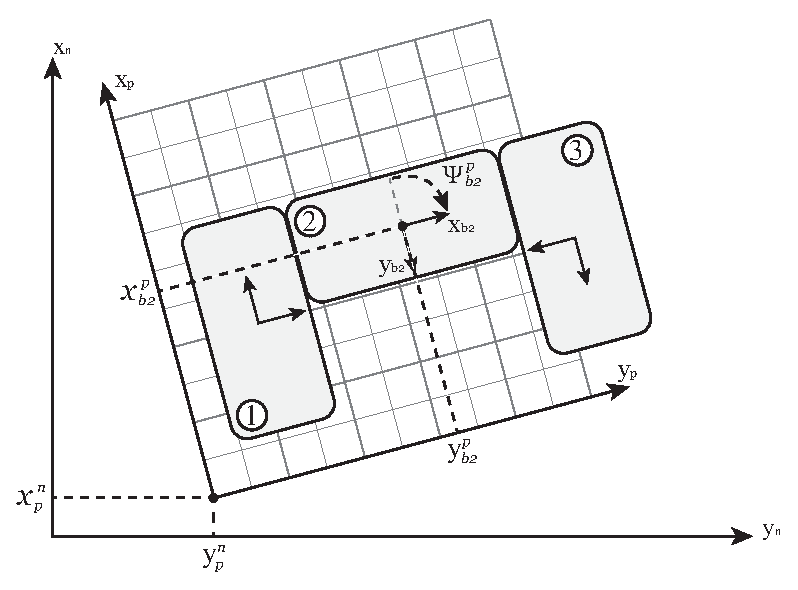
\includegraphics[width=0.8\textwidth]{ned_platform_frame}
	\caption{A platform consisting of three modules. Expression of pose of vessel 2 in the platform coordinate system ($ \{p\}$) is illustrated, as well as position of the platform frame origin in global ($ \{n\}$) frame. This example shows the origin of the platform coordinate system outside of the physical body of the platform, but this placement can be chosen elsewhere at the convenience of the designer.}
	\label{fig:bartned_platform_frame}
\end{figure}

Each module $m_i$ has $r_i = 0,1,2,...$ actuators that are able to impose forces on that module to move it, such as propellers. The amount of actuators that modules have may not be equal for all vessels. This may be unequal by design (as in a heterogenous fleet) , or as a response to a noticed malfunctioning thruster. The total amount of actuators is the summation of the actuators of all vessels.

\begin{equation} 
r =\sum_{i=1}^{n} r_i
\end{equation}

Actuators are bound to various constraints such as direction and maximum force output. Acuators that make forces between vessels to connect them could be described as actuators as well, which can be benificial if connections are not considered rigid. Actuators have dynamics of their own, meaning that they often do not respond instantaneous. However, modelling the dynamics of actuators can  overcomplicate a total system model. If a model is to be kept simple, one can assume that execution of actuator reference is done sufficiently accurate and timely. It is a good idea to reflect if this assumption is reasonable by evaluating the performance of used actuators to accurately follow control inputs, and judge whether inacurracy or delay will significantly affect overall system behavior. 

\subsection{Motion control systems}
Waterborn vehicle dynamics can be described according to \citet{fossen2011handbook}, where the author shows that translational motion of a vessel about CO satisfies

\begin{equation}
m [ \dot{\textbf{v}}_{b/n}^{b} + \dot{\omega}_{b/n}^{b}  \times \textbf{r}_g^b     + \omega_{b/n}^{b}  \times  \textbf{v}_{b/n}^{b} +  \omega_{b/n}^{b}  \times ( \omega_{b/n}^{b}  \times \textbf{r}_g^b   ) ] = \textbf{f}_b^b
\label{eq:fossen2011TranslationalMotionAboutCO-eqnumber-3-33}
\end{equation}

and that rotational motion of a vessel about CO satisfies

\begin{equation} 
\textbf{I}_b  \dot{\omega}_{b/n}^{b} + \omega_{b/n}^{b}  \times \textbf{I}_b \omega_{b/n}^{b}  + m \textbf{r}_g^b \times  ( \dot{\textbf{v}}_{b/n}^{b} +   	\omega_{b/n}^{b} 	 \times	\textbf{v}_{b/n}^{b}	) = \textbf{m}_b^b 
\label{eq:fossen2011RotationalMotionAboutCO-eqnumber-3-40} 
\end{equation}

where components in equation \ref{eq:fossen2011TranslationalMotionAboutCO-eqnumber-3-33} and \ref{eq:fossen2011RotationalMotionAboutCO-eqnumber-3-40} are defined as

\begin{table}[H]
	\centering
	\begin{tabular}{llll}
		$\boldmath{f}^{b}_{b} $ 	   	& = & $[X,Y,Z]^\top$ 		&	- Force with line of action through point $o_b$ expressed in coordinate system $\{b\}$ \\[5pt]
		$\boldmath{m}^{b}_{b} $   		& = & $[K,M,N]^\top$ 		&	- Moment about point $o_b$ expressed in coordinate system $\{b\}$ \\[5pt]
		$ \textbf{v}^{b}_{b/n}$   		& = & $[u,v,w]^\top$ 		&	- Linear velocity of point $o_b$ with respect to $o_n$ expressed in coordinate system $\{b\}$ \\[5pt]
		$ \omega^{b}_{b/n}$   			& = & $[p,q,r]^\top$ 		&	- Angular velocity of $\{b\}$ with respect to $\{n\}$ expressed in coordinate system $\{b\}$  \\[5pt]
		$\textbf{r}^{b}_{g} $ 			& = & $[x_g,y_g,z_g]^\top$ 	&	- Position of centre of gravity expressed in coordinate system $\{b\}$ 
	\end{tabular}
\end{table}

\citet{fossen1994guidance} expresses equation \ref{eq:fossen2011TranslationalMotionAboutCO-eqnumber-3-33} and \ref{eq:fossen2011RotationalMotionAboutCO-eqnumber-3-40} vectorial form
\begin{equation}
\textbf{M}_{RB} \dot{\nu} + \textbf{C}_{RB}(\nu)\nu  = \tau_{RB}
\label{eq:fossen1994RigidBodyKinetics1}
\end{equation}

where $ \textbf{M}_{RB} $ is the rigid body inertia matrix, $\textbf{C}_{RB}$ is a matrix of rigid-body Coriolis and centripetal forces due to the rotation of $\{b\}$ about the inertial frame $\{n\}$, $\nu$ is a vector with generalized velocities expressed in $\{b\}$ and $\tau_{RB}$ is a vector with generalized forces expressed in $\{b\}$. 

Dampening forces can be modelled linear with constant D matrix as 
\begin{equation}
\textbf{M}_{RB} \dot{\nu} + \textbf{C}_{RB}(\nu)\nu  + \textbf{D}\nu = \tau
\label{eq:fossen1994RigidBodyKineticsinclDampeningLinear}
\end{equation}


Or nonlinear as: 
\begin{equation}
\textbf{M}_{RB} \dot{\nu} + \textbf{C}_{RB}(\nu)\nu  + \textbf{D}(\nu)\nu = \tau
\label{eq:fossen1994RigidBodyKineticsinclDampeningNonLinear}
\end{equation}
Which can both be estimated by model identification experiments. Whether linear or nonlinear dampening models are suitable depends on the accuracy of tests and reasonabe operating range. It is common to model some hydrodynamic forces as constant additive accelleration coefficients. \citet{humphreys1978prediction} states that the forces and moments represented by the acceleration hydrodynamic coefficients can, to a very great extent, be modeled as potential flow phenomena, yielding 

\begin{equation}
\textbf{M} \dot{\nu} + \textbf{C}(\nu)\nu  + \textbf{D}(\nu)\nu = \tau{}
\label{eq:fossen1994RigidBodyKineticsinclAddedMass}
\end{equation}

where
\begin{equation}
\textbf{M} = \textbf{M}_{RB} + \textbf{M}_{A}
\end{equation}
Where $ \textbf{M}_{RB} $ represents inertia of the rigid module and $\textbf{M}_{A}$ represents hydrodynamic added mass. Similarly
\begin{equation}
\textbf{C}(\nu)\nu = \textbf{C}_{RB}(\nu)\nu + \textbf{C}_{A}(\nu)\nu
\end{equation}
Where $ \textbf{C}_{RB}(\nu)\nu $ and $\textbf{C}_{A}(\nu)\nu$ represent coriolis and centripetal forces of the rigid body and hydrodynamic added mass. 

Control forces of all actuators (of all modules) can be described in a vector format as:
\begin{equation}
\textbf{f} = [F_{1},F_{2},F_{3}, ... F_{r}]^\top
\end{equation}
Where $F_i$ is the control force generated by actuator $r_i$. 
If the relation between control input and resulting force can be assumed linear, the control forces can be expressed as:

\begin{equation}
\textbf{f} = \textbf{K} * \textbf{u}
\end{equation}

Where $\textbf{u}$ is a vector of control inputs and $\textbf{K}$ is a diagonal force coefficient matrix (see \citet{fossen2011handbook})

Control forces applied across the body can be expressed in total control forces:
\begin{equation}
\tau = \textbf{T}(\alpha)\textbf{f}
\end{equation}
Where $ \textbf{T}(\alpha) \in \mathbb{R}^{n\times r}$ is the thrust configuration matrix, dependent on angles $ \alpha = [\alpha_1,... \alpha_p]^\top \in \mathbb{R}^{p}$ of p rotatable thrusters. \citet{fossen2011handbook} shows how the use of angles of rotatable thrusters can be avoided in the above expression by decoupling the force of a rotatable thruster in two separate forces (generaly decoupled in x and y for surface vessels). Decoupling x and y components of a rotating thruster can simplify math challenges, but does require to take into account physical constraints of absolute maximum thrust of the actuator. 



The team of connected modules has a single, dynamic, multi-robot task, namely the control of actuators to satisfy a time varying platform state. What a satisfactory state actually is depends on the designer, but this is usually defined as a reference state, such as desired positions, and/or velocities.  Utilizing the concept of a reference state in a multi-robot collaborative system means that the controlling entity of a module or platform needs means to aquire the control objective. Various design options are possible to have a set of robots collaborating towards  achieving a single goal. The control objective can be created by various entities.
\begin{itemize}
	\item The robot can generate its own control objective, sensing the environment and following a decision protocol. 
	\item The control objective can be generated by another entity, such as another robot or an operator. This would require means of communication. 
\end{itemize}

\citet{parasuraman2000model} describes an approach on dividing a control problem in four stages with similarities to human decision making. This approach is general and intended to be applicable to a wide spectrum of robot systems, as shown in figure \ref{fig:parasuraman2000model-foursteps}, yet can be applied to a multi-robot system as well. The amount of agents in the multi robot system that collaboratively perform functionality of one of the stages can vary. Some tasks can be done by a single agent, while other tasks can be achieved with multiple. For example; sensing fleet state can be done by a single centralized agent, sending sensor data to on board decision makers, or each vessel can have its own means of sensing its surroundings. 
%\colorbox{yellow}{\parbox{12cm}{This is a very }}\\
%"The first stage refers to the acquisition and registration of multiple sources of information. This stage includes the positioning and orienting of sensory receptors, sensory processing, initial pre-processing of data prior to full perception, and selective attention. The second stage involves conscious perception, and manipulation of processed and retrieved information in working memory [13]. This stage also includes cognitive operations such as rehearsal, integration and inference, but these operations occur prior to the point of decision. The third stage is where decisions are reached based on such cognitive processing. The fourth and final stage involves the implementation of a response or action consistent with the decision choice." \cite{parasuraman2000model}

A collaborative multi vessel control system can thus have its tasks distributed across agents in many ways. To control $n$ vessels where each vessel is equipped with $r_i$ actuators, the following system components can be identified for a certain design divided as shown in \citet{parasuraman2000model}
\begin{itemize}
	\item i agents that aquire information about the state, or called sensing.
	\item j agents that interpret sensed information, converting it into concepts, such as a state estimate. 
	\item k agents that formulate sets of control options
	\item l agents that decide a control option from the set
\end{itemize}

\begin{figure}[H]
	\centering
	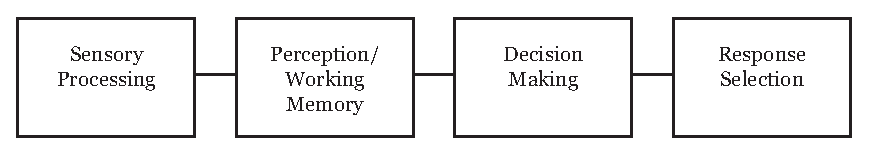
\includegraphics[width=0.8\textwidth]{parasuraman2000model-foursteps}
	\caption{Four-stage model of human information processing. \cite{parasuraman2000model}}
	\label{fig:parasuraman2000model-foursteps}
\end{figure}

Classic marine control theory pertains only a single ship. A common division of the overall control system into subsystems is according to the Guidance, Navigation and Control (GNC) scheme \cite{fossen2011handbook}. The navigation system uses sensors and an observer to generate a state estimate. The guidance system performs task planning and continuously generates a control objective or reference. This is used by the (motion) control system to coordinate responses of available actuators, such that the vessel response follows the reference. 

\subsection{Multi-robot Cooperation}
Various challenges in cooperative multi robot systems are systematically described in existing literature. A section of relevant terms and concepts will be discussed to adress the problem of this section. 

For a multi-robot system, the division of tasks to a set of robots is referred to as "task allocation" \citet{lerman2006analysis}. This is extended to "dynamic task allocation" if the assignment of tasks to robots needs to be adjusted continuously due to changes in task environment and system response. 
\citet{lerman2006analysis} describes a "distributed multi-robot system" as a MRS that does not have a central coordinator. Distribution and centralization of control structure both have their benefits and disadvantages. Decisions in distributed control systems need to be made with incomplete information, while a centralized decision making agent has the potential to use all available data. Centralized control structures have, however, a single point of failure and can encounter scaling issues. 

As multiple robots collaboratively seek to perform the common task of platform motion control, there are varying approaches to allocating control efforts with similar results, as a vessel platforms actuators are likely far more numerous than the (debatably consistent) degrees of freedom. \citet{fossen2011handbook} shows how a vessel motion control block is commonly divided into a dedicated subsystem that generates 'control efforts', and a block that allocates the desired control effort, by dividing it over the available actuators, schematically shown in figure \ref{fig:fossenControlAllocationPNG}. This approach is also used for the configuration adaptive vessel platform controller in \citet{park2019coordinated}, while therein control allocation is referred to as "coordination" and generation of control efforts is referred to as "robust control". 

 \begin{figure}[h!]
 	\centering
 	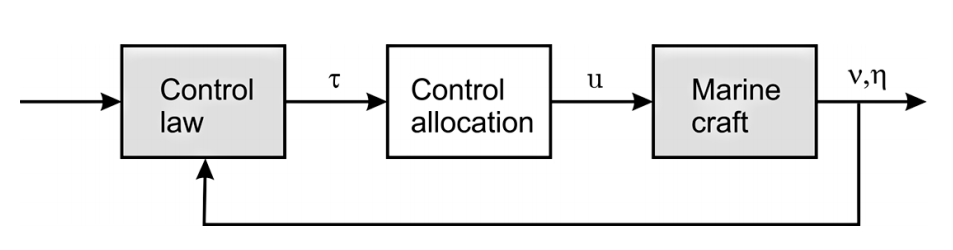
\includegraphics[width=0.6\textwidth]{fossen2011handbookControlAllocation}
 	\caption{Block diagram showing the control-allocation-block in a vessel motion control system. \cite{fossen2011handbook}.}
 	\label{fig:fossenControlAllocationPNG}
 \end{figure}
 
To use this methodology for control of vessel platform motion, the state estimation would need to pertain platform state, and not that of an individual vessel. This is generally positions $\eta_p$ and possibly velocities $\nu_p$, which are to be controlled to a desired state. Which parts of the state are to be controlled depends on the approach and complexity of the control system. Dynamic positioning, for instance, controls pose ($\eta = [x,y,\Psi]$) but not directly velocities ($\nu = [u,v,r]$).

\citet{park2019coordinated} utilizes a centralized control approach to generate control efforts that need to be applied on the platform, while their approach assumes rigid connections. Control effort generation was achieved by means of a PI controller. Control decisions are made centralized on one vessel that is elected as coordinator, which divides the control effort over platform modules. A schematic of the control loop of \citet{park2019coordinated} is  shown in figure \ref{fig:park2019coordinatedSontrolScheme}, showing various elements that could be sensibly interpreted with both the four stage model of \citet{parasuraman2000model} and the GNC scheme as described by \citet{fossen2011handbook}.

\begin{figure}[H]
	\centering
	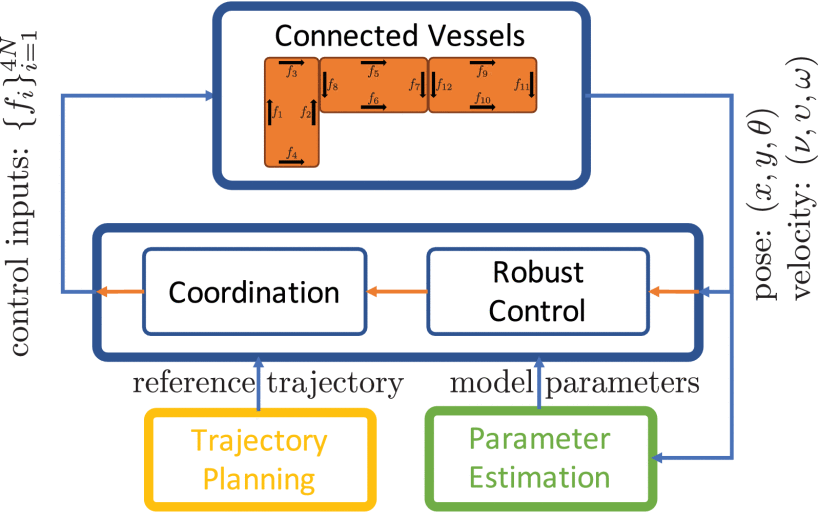
\includegraphics[width=0.6\textwidth]{park2019coordinatedSontrolScheme}
	\caption{Multi-vessel navigation system that consists of parameter estimation, trajectory planning, and coordinated robust control. \cite{park2019coordinated}. Note that the reference trajectory signal is not fed into the coordination block, although it might be interpreted as such on a first glance.}
	\label{fig:park2019coordinatedSontrolScheme}
\end{figure}
\section{Effects of combining systems}
\label{analysisCombined}
The previous sections discussed system analysis of modular surface vessel platforming systems that perform automated reconfiguration (section \ref{analysisReconfiguration}), and configuration adaptive platform control approaches (section \ref{analysisConfigAdaptation}).
This section combines the analysis presented on these two systems by assessing how the functionality of these two systems can be combined. Various design considerations have been identified of which some will be discussed again in this section in a more pragmatic way. Fundamental requirements to achieve the system demands will be presented, yet more emphasis will be given on predicting what choices will be more relevant for commercial logistic applications instead of general robotics. 


\subsection{Requirements}
In order to realize both behaviors, various subfunctions have been identified in section \ref{analysisConfigAdaptation} and \ref{analysisReconfiguration}, which are summarized. Table \ref{tab:assemblyCharacteristicsSummed} presents characteristics of a system that performs Automatic vessel platform reconfiguration, together with the approach and design choices of projects that published about such systems. A similar table on characteristics of vessel platform systems that perform configuration adaptive control strategies are shown in table \ref{tab:adaptiveCharacteristicsSummed}:

\begin{table}[H]
	\centering
	\begin{adjustbox}{width=1\textwidth}
		\begin{tabular}{|l|l|l|l|}
			\hline		
			\begin{tabular}[c]{@{}l@{}}Fundamental Characteristic \\ or requirement \end{tabular} & Roboat project \cite{kelly2019algorithms} \cite{mateos2019autonomous} & \begin{tabular}[c]{@{}l@{}} ISO container module assembly \\ project \cite{o2014self} \cite{paulos2015automated}\end{tabular} & Notes \\ \specialrule{1.5pt}{1pt}{1pt}
			
			A set of modules & Homogeneous fleet  &  Homogeneous fleet  & 	\begin{tabular}[c]{@{}l@{}} Approaches and goals of implementing heterogenous and \\ homogeneous systems differ significantly. \end{tabular} \\ \hline
			
			A strategy to reconfigure. & Deterministic& Deterministic & \begin{tabular}[c]{@{}l@{}}  Various approaches are possible which can be categorized as stochastic \\ or deterministic \end{tabular}\\ \hline
			
			Means of repositioning modules  & \begin{tabular}[c]{@{}l@{}}Cross shaped non roatable\\ thruster setup. Individual \\ vessels are fully actuated \end{tabular} & \begin{tabular}[c]{@{}l@{}}Plus shaped non roatable\\ thruster setup. Individual \\ vessels are fully actuated \end{tabular} & \begin{tabular}[c]{@{}l@{}} Modules can be designed to perform independent or with help from \\ other agents. Individual modules can be under- or fully actuaded, while \\ the observed trend is towards the latter. \end{tabular} \\ \hline
			
			Means of maintaining configuration  & 
			\begin{tabular}[c]{@{}l@{}}Physical ball-cone joint  \\ connection \cite{mateos2019autonomous} or by means \\ of magnets \end{tabular}  &
			\begin{tabular}[c]{@{}l@{}}Physical rope-hook joint \\ connection. Variable \\ stiffness \end{tabular}  & 
			Various solutions are possible, depending on scale, goal and environment. \\ \hline
			
		\end{tabular}
	\end{adjustbox}
	\caption{Fundamental characteristics on automated modular vessel platform reconfiguration systems}
	\label{tab:assemblyCharacteristicsSummed}
\end{table}

\begin{table}[H]
	\centering
	\begin{adjustbox}{width=1\textwidth}
		\begin{tabular}{|l|l|l|}
			\hline		
			\begin{tabular}[c]{@{}l@{}}Fundamental Characteristic \\ or requirement \end{tabular}  & \citet{park2019coordinated}  &  Notes \\ \specialrule{1.5pt}{1pt}{1pt}
			
			Connected robots share a single objective & The platforms position is given as a reference. & \begin{tabular}[c]{@{}l@{}} Other approaches may also attempt to more directly \\ control speed besides position, or integrate higher \\ level planning (e.g. guidance) tasks.\end{tabular} \\ \hline
				
			Robot actions are coordinated  & \begin{tabular}[c]{@{}l@{}} A platform has a centralized controller,\\ deciding and coordinating all connected modules. \end{tabular} & \begin{tabular}[c]{@{}l@{}} Coordinated behavior is aimed to improve\\ performance with respect to the sum of individuals, \\ yet comes at the cost of increased complexity. \end{tabular}\\ \hline
		
			\begin{tabular}[c]{@{}l@{}} The decision making protocol functions\\ on a wide variety of configurations \end{tabular}  & \begin{tabular}[c]{@{}l@{}} Control approach uses an approximate model based \\ on the number of connected modules (however, not \\ the  configuration shape). The control system yields \\ a single control effort for the entire platform that is \\ subsequently distributed among modules. \end{tabular} & \begin{tabular}[c]{@{}l@{}} Criteria of motion control performance will \\ vary between usecases, as well as the amount of\\ considered configurations.   \end{tabular} \\ \hline
			
			
			
		\end{tabular}
	\end{adjustbox}
	\caption{Fundamental characteristics on collaborative and coordinated vessel-platform motion control systems}
	\label{tab:adaptiveCharacteristicsSummed}
\end{table}


An additional characteristic is identified as these two behaviors are integrated in one framework. As a platform configuration changes through time, the motion control system needs to be able to support real time varying configuration parameter, such as estimated dynamics, size, shape, or centre of mass, or in some cases even the network topology. 

\subsection{Common Considerations}
Various considerations for multi robot systems have been observed as key to characterizing a design and are discussed here.

Choosing centralized or decentralized control structures affect many design options for both platform asembly and control. Decentralization generally facilitates great scalability, such that they can be deployed at small scale and in great numbers. A centralized entity can however make decisions based on a more complete state of the overall system, and make more effective decisions. Centralized systems have a single point of failure, which can be undesirable. Centralized systems are also reliant on a communication network with a certain reliability, latency and bandwith.

Homogeneous robot systems consist of robots which are designed to be similar, while heterogeneous systems have modules equipped with different shape, size or abilities. Heterogenous robots can use a wider variety of features without adding too many features per module, although a system topology can get more complex. Homogeneous robots can be interchanged by any other if desired, and are possibly easier to produce in large numbers. All sources that published results on systems that performed automated reconfiguration and configuration adaptive control have been applied using a homogenous fleet.

Vessels that operate individually can be underactuated or fully actuated. Control of underactuated systems is generally more complex, though not impossible. \citet{ashrafiuon2010review} reviews different approaches of controlling automated  underactuated surface vessels. This work focusses on control approaches which are categorized in "setpoint", "trajectory tracking" and "path following" approaches. Light is shed on advantages and disadvantages of various mentioned approaches. It is convenient to have fully actuated modules for vessel platforming purposes, which is shown to be feasible by projects that use fully actuated vessels for both automated reconfiguration and configuration adaptive control. 

Designing towards utilizing extensive amounts of communication in a multi robot system drastically changes availability of further design options. A vessel system connected into a network that continuously shares information can become reliant on the presence and performance of the network. Facilitating connectivity comes to cost at various facets. Modules need this extra feature built in, which makes a module more complex, expensive, power consuming, while adding another component that can break. Nihilistic approaches that only add essential features to a module will increase scalability, due to low cost, replacability and reliability. 


To facilitate collaborative platform control, some communication between operator and module is always necessary, as the task of the platform needs to be communicated from human to the vessel system. Many multi robot systems that are nowadays developed often have a high reliance on communication network availability, as task distribution has many benefits and opens up new doors in terms of design choices and possible emergent behaviors. 

\vspace{5mm}

This chapter explored the meaning two behaviors of automated vessel platform control systems reffered to as 'automated reconfiguration' and 'collaborative and coordinated platform motion control'. Various approaches to describing and designing such systems were discussed to deepen understanding of the behaviors and broaden the view on potential design solutions. Fundamental characteristics of both evaluated systems have been identified to aid development of a framework integrating the two in the next chapter. 







	\chapter{Multi-vessel System State Description}
\label{chap:stateDescription}
This chapter builds on existing vessel state descriptions to formulate a multi-vessel state description. Furthermore, a novel approach to predict multi-vessel platform dynamics from individual models is proposed to  answer the research subquestion:

\begin{itemize}
	\item How can the dynamics of the multi-vessel system be represented?
\end{itemize}
The described multi-vessel state description as described in Sec. \ref{sec:notations} aims to enable consistent system notation of scenarios pertaining more than a single vessel, as mult-vessel frameworks have more objects that can be referred to. The concept and definition of a platform-coordinate system is also introduced.

For collaborative motion control of modular objects an approximate dynamical model is often desired. As model parameter estimation experiments are often infeasible for every configuration of a combined structure, a prediction of dynamical behavior is proposed using the often known dynamics of modules in Sec. \ref{platformModel}

\section{System State Notations} 
\label{sec:notations}
A sensible notation of a system aids implementation and consistent discussion of motion control systems. Vessel automation is a topic where robotic and maritime science overlap. System description of vessel systems from a control perspective is described in \citet{fossen2011handbook}, which are used as a foundation of the multi-vessel state description

\subsection{Single vessel state description}
For control purposes, ships are generally considered rigid bodies. A rigid body has 6 degrees of freedom (DOF) in which can all be evaluated or simplified to a reduced set of motions such as 3-DOF planar motion. For ships, this is commonly expressed according to the notation of \citet{sname1950nomenclature} with respect to various coordinate systems. Components of orientation, velocities and forces are shown in table \ref{tableSname}.

\begin{table}[h!]
	\centering
	\begin{tabular}{|l|l|l|l|l|}
		\hline
		DOF & & \begin{tabular}[c]{@{}l@{}}Positions and \\ Euler Angles\end{tabular} & \begin{tabular}[c]{@{}l@{}}Linear and \\ angular Velocities\end{tabular}   & \begin{tabular}[c]{@{}l@{}}Forces and \\ Moments\end{tabular}  \\ \hline
		1&	Surge      & x                    & u          & X                  \\ \hline
		2&	Sway       & y                    & v          & Y                  \\ \hline
		3&	Heave      & z                    & w          & Z                  \\ \hline
		4&	Roll       & $\phi $                 & p          & K                  \\ \hline
		5&	Pitch      & $\theta  $              & q          & M                  \\ \hline
		6&	Yaw        & $\psi  $                & r          & N                \\ \hline
		
	\end{tabular}
	\caption{SNAME notation for marine vessels}
	\label{tableSname}
\end{table}

A North-East-Down coordinate system will be used as reference to a global coordinate system as $\{n\}$, while a body fixed coordinate system is referred to with $\{b\}$. This body fixed frame defines the motion of the vessel, such that every position or speed of a vessel is defined in the motion of the body frame. Figure \ref{figsname} shows vessel motions expressed on the body fixed frame. Motion of surface vessels is commonly simplified to 3 degrees of freedom in the surface plane, as is shown in figure \ref{fig:delfiaBodyFrame1}. This assumes effects of heave, roll and pitch can be neglected. This simplification of planar motion is adopted for the developed control system in this paper as described in Chap. \ref{chap:sysDevelopent}. 

\begin{figure}[h!]
	\centering
	\makebox[\textwidth][c]{
		\begin{minipage}{0.45\textwidth}
	\centering
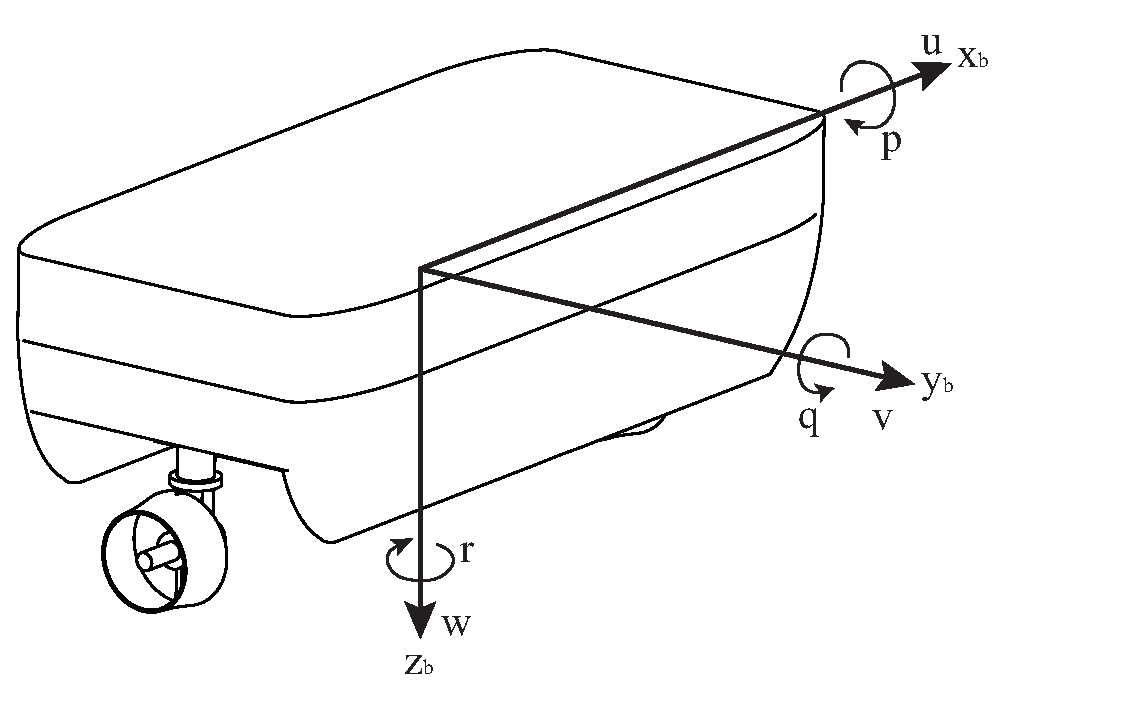
\includegraphics[width=1.0\textwidth]{DelfiaSname.eps}
\caption{Six degrees of motion depicted of a Delfia vessel expressed with respect to the body-fixed coordinate system $\{b\}$ in convention with \citet{sname1950nomenclature}}
\label{figsname}
		\end{minipage}\hfill
		\begin{minipage}{0.45\textwidth}
	\centering
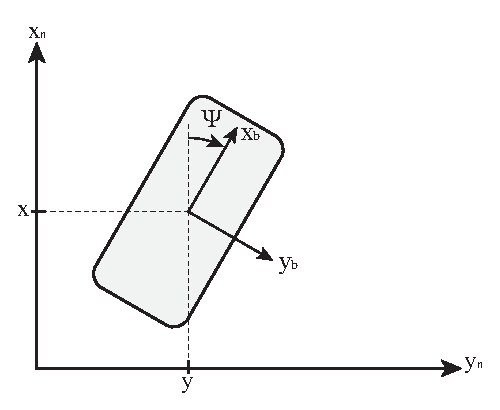
\includegraphics[width=1.0\textwidth]{delfia_bodyframe1.eps}
\caption{Three degrees of freedom depicted as only motion in the surface plane is considered}
\label{fig:delfiaBodyFrame1}
		\end{minipage}
	}
\end{figure}

Position, orientation, velocities, forces and moments are further noted as:
\begin{table}[H]
\centering
\begin{tabular}{lll}
		$\textbf{p}^{i}_{j} $ 			& = &  	Position of point $j$ expressed in coordinate system $\{i\}$ \\[5pt]
		$\Theta_{ij}$ 					& = & 	Euler angles between coordinate systems $\{i\}$ and $\{j\}$ \\[5pt]
		$ \textbf{v}^{k}_{i/j}$   		& = & 	Linear velocity of point i with respect to j expressed in coordinate system $\{k\}$ \\[5pt]
		$ \omega^{k}_{i/j}$   			& = &	Angular velocity of object i with respect to j expressed in coordinate system $\{k\}$  \\[5pt]
		$\boldmath{f}^{i}_{j} $ 	   	& = &	Force with line of action through point $j$ expressed in coordinate system $\{i\}$ \\[5pt]
		$\boldmath{m}^{i}_{j} $   		& = & 	Moment about point $j$ expressed in coordinate system $\{i\}$
\end{tabular}
\end{table}

As a result of the reduction from 6 to 3 degrees of freedom, vectorial expressions of our system become:
\begin{table}[H]
	\centering
	\begin{tabular}{llllllll}
		NED position & $\textbf{p}^{n}_{b} $ & = & $  \begin{bmatrix} x^{n}_{b} \\[5pt] y^{n}_{b} \end{bmatrix}$ & 
		Attitude (Euler angles) & $\Theta_{nb} $ & = & $ \begin{bmatrix} \Psi^n_b \end{bmatrix}$   \\[20pt] %\begin{bmatrix} N \\ E \end{bmatrix} =
		\begin{tabular}[c]{@{}l@{}}Body-fixed \\ linear velocity \end{tabular} & $ \textbf{v}^{b}_{b/n} $ & = & $ \begin{bmatrix} u \\ v \end{bmatrix} $ & 
		\begin{tabular}[c]{@{}l@{}}Body-fixed \\ angular velocity \end{tabular} & $ \omega^{b}_{b/n} $ & = & $ \begin{bmatrix} r \end{bmatrix} $ \\[20pt]
		\begin{tabular}[c]{@{}l@{}}Body-fixed \\ force \end{tabular} & $\boldmath{f}^{b}_{b} $ & = & $ \begin{bmatrix} X \\ Y \end{bmatrix} $ & 
		\begin{tabular}[c]{@{}l@{}}Body-fixed \\ moment \end{tabular} & $\boldmath{m}^{b}_{b} $ & = & $ \begin{bmatrix} N \end{bmatrix} $ 
	\end{tabular}
\end{table}


General motion of vessels in 3 degrees of freedom are described by the following generalized positions and velocities \cite{fossen2011handbook}

\begin{equation}
	\eta = \begin{bmatrix} \textbf{p}^{n}_{b} \\[8pt]  \Theta_{nb} \end{bmatrix} = \begin{bmatrix} x^{n}_{b} \\[8pt]  y^{n}_{b} \\[8pt] \Psi^n_b \end{bmatrix}
	\label{generalizedPos1}
\end{equation}

\begin{equation}
	\nu = \begin{bmatrix} \textbf{v}^{b}_{b/n} \\[8pt]  \omega^{b}_{b/n} \end{bmatrix} = \begin{bmatrix} u\\v\\r \end{bmatrix}
	\label{generalizedVel1}
\end{equation}

\begin{equation}
	\tau = \begin{bmatrix} \boldmath{f}^{b}_{b} \\[8pt]  \boldmath{m}^{b}_{b} \end{bmatrix} = \begin{bmatrix} X \\ Y \\ N \end{bmatrix}
	\label{generalizedFor1}
\end{equation}

Where $\eta$ describes orientation, $\nu$ describes velocities and $\tau$ describes forces acting upon the system. 
To avoid clutter, when it is deemed clear to in which reference frame a position or velocity is expressed, the subscript and superscript will not always be shown. This is for instance the case for generalized positions as in equation \ref{generalizedPos1} that is most of the time with respect to $\{n\}$ such that it is just expressed in $ [x,y,\Psi]^\top$. By default, $ \nu$, $\tau$ are expressed in $\{b\}$, and $\eta$ is described in $\{n\}$.

Velocities expressed in $\{b\}$ and $\{n\}$ frame are related as:

\begin{equation}
\dot{\eta} = R(\Psi)\nu
\end{equation}

Where $R$ is the rotation matrix of $\Psi$ around the z axis. For pure motion in the 3 surface plane degrees of freedom, this becomes:

\begin{equation}
R(\Psi) = \begin{bmatrix} cos(\Psi) & -sin(\Psi) & 0  \\ sin(\Psi) & cos(\Psi) & 0 \\ 0 & 0 & 1 \end{bmatrix}
\end{equation}

Coordinate system origin and centre of mass are referred to as:

\begin{table}[H]
	\centering
	\begin{tabular}{lll}
		$\textbf{o}_{i}^{j} $ 			& = &  	Origin of coordinate system $i$ expressed in coordinate system $\{j\}$ \\[10pt]
		$\textbf{p}_{cm}^{i} $ 			& = &  	Position of the centre of mass expressed in coordinate system $\{i\}$ \\
	\end{tabular}
\end{table}


\subsection{Multivessel system notation}
As fleet systems transition from describing a single vessel to a system of many, it becomes necessary to differentiate between local frames of different vessels. We change subscripts referencing to a single vessel to a notation for $n$ vessels. For example, referencing to a single body coordinate system as $\{b\}$ changes to $\{b1\},\{b2\},\{b2\} \dots \{bn\}$ in order to indicate which body frame is referenced to. Relative orientations and velocities are considered to become more relevant as vessels have to operate in proximity or even contact to realize assembly into platforms. Figure \ref{fig:localframeShowing} illustrates how position of a vessel can be described in a local body fixed frame, which may be more relevant and intuitive for automated assembly purposes. The position of origin of body 2 expressed in $\{b1\}$ illustrated in figure \ref{fig:localframeShowing} becomes:

\begin{equation}
\textbf{o}_{b1}^{b2} = \begin{bmatrix}x_{b1}^{b2} \\[10pt] y_{b1}^{b2} \end{bmatrix}
\end{equation}

Furthermore, the notations of motion shown in equation \ref{generalizedPos1}, \ref{generalizedVel1} and \ref{generalizedFor1} by default refer to a specific frame. Pose $\eta$ is expressed globally in $\{n\}$. Velocities $\nu$ and  forces $\tau$ are expressed in the body fixed frame $\{b\}$. It can be convenient to express motions to different frames as well. Take the example of two moving vessels docking to eachother while moving. To answer the question "How close is a vessel to a docking position?" a relative expression of position is required. The convention of subscripting to refer to a coordinate system is extended to $\eta$, $\nu$ and $\tau$ as well as follows:

\begin{equation}
\eta_b^n = \begin{bmatrix} \textbf{p}^{n}_{b} \\[8pt]  \Theta_{nb} \end{bmatrix} = \begin{bmatrix} x^{n}_{b} \\[8pt]  y^{n}_{b} \\[8pt] \Psi^n_b \end{bmatrix}
\label{generalizedPos2}
\end{equation}

Where the sub- and superscript of $\eta_b^n$ refer to object $b$ expressed in $\{n\}$. This convention allows expression of relative motion between vessels by writing $\eta_{b2}^{b1}$ which indicates pose of body 2 expressed in the local frame of body 1, also illustrated in \ref{fig:localframeShowing}. Note that velocities and forces are regularly referred to as "body-fixed", but that is not necessarily the case anymore with this convention. 

\begin{figure}[h!]
	\centering
	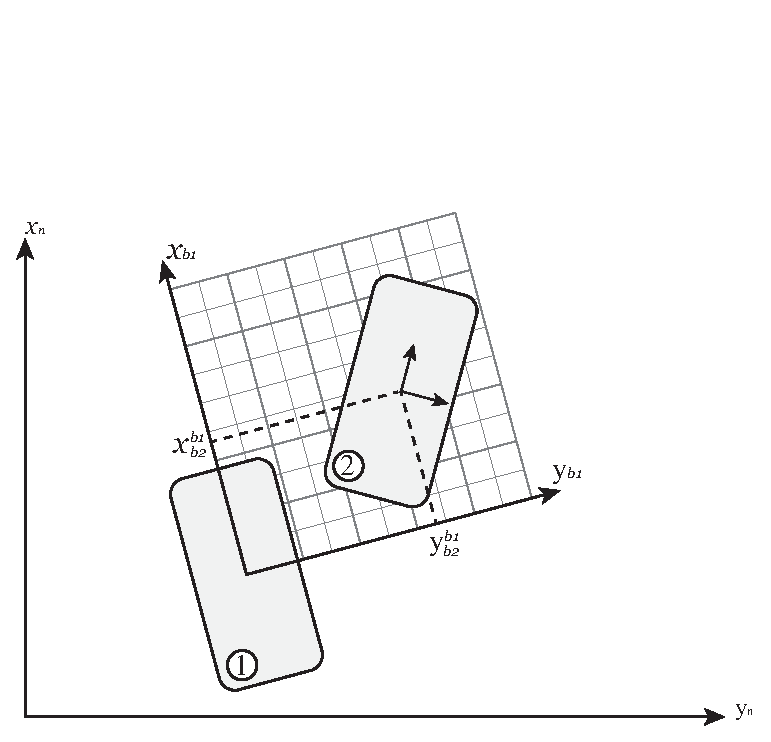
\includegraphics[width=0.6\textwidth]{localframeShowing.eps}
	\caption{Two vessels are shown from above, illustrating interpretation of expressing a module's state (of module 2) in another module's body-fixed coordinate system (of module 1).}
	\label{fig:localframeShowing}
\end{figure}
\newpage

\section{Dynamical model of a Platform}
\label{platformModel}
An approximate model for the platform dynamics is used by the platform controller in the process of generating control effort. When the platform control agent is notified that its configuration is changed, it recomputes various parameters for the dynamical model that describe the new rigid body dynamics.
The platform control agent keeps track of the following 
\begin{itemize}
	\item Connectivity of modules
	\item Configured pose connected modules
	\item Parameters that describe dynamics of individual modules
\end{itemize}

Use-cases where vessel assemblies are formed in many varying configurations can make experimental model parameterization infeasible for all reasonably forseeable configurations.  Predicting a dynamical model by combining models of modules can provide a quick, cheap and scalable solution with respect to performing parameter estimation experiments. 
The approach to estimating the dynamical model of a platform is explained in this section, but also more elaborately described and discussed in appendix \ref{appendix:CombineDynamics}

A dynamic model of the platform is formed by expressing all models of the modules in the same point and coordinate system, which are then combined. It is shown how terms from multiple module models can be grouped for convenient expression, and how the centre of mass of the combined structure can be found. 

Models of modules are expressed in platform frame origin by (1) translating the expressions to $o_{p}$ as a reference point and (2) rotating the expressions to match  coordinate system $\{p\}$. This approach works also for models of which the origonal inertial matrix is not defined in the CG, and/or for models that have directional dependent mass (e.g., hydrodynamic added mass). 

Generalized positions and velocities of the platform are described respectively as
\begin{equation}
	\eta_{p/n}^{n} = \begin{bmatrix} \textbf{p}^{n}_{p} \\[8pt]  \Theta_{np} \end{bmatrix}
\end{equation}
\begin{equation}
	\nu_{p/n}^{p} = \begin{bmatrix} \textbf{v}^{p}_{p/n} \\[8pt]  \omega^{p}_{p/n} \end{bmatrix}
\end{equation}

\begin{figure}[H]
	\centering
	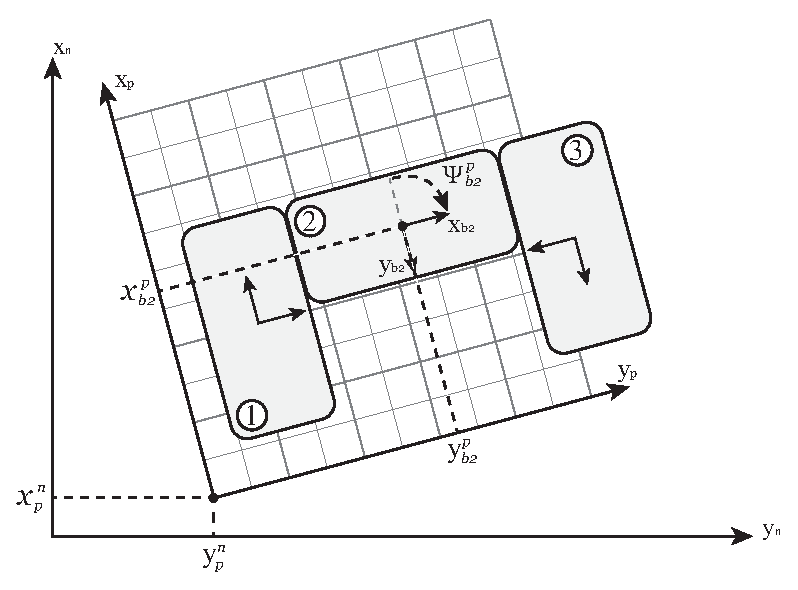
\includegraphics[width=0.7\textwidth]{ned_platform_frame}
	\caption{An assembly of three vessels in 2d. Components from equation \ref{eq:moduleStaticPlacementEtaDefinition} that define configured pose of vessel 2 in the platform coordinate system ($ \{p\}$) are illustrated, as well as position of the platform frame origin in ($ \{n\}$)}
\end{figure}

The placement of all vessels (defined by the position and orientation of coordinate system $\{b\}$) within the assembly is known and can be described with respect to $\{p\}$ expressed in $\{p\}$ as
\begin{equation}
	\eta_{b/p}^{p} = \begin{bmatrix} \textbf{p}^{p}_{b} \\[8pt]  \Theta_{pb} \end{bmatrix}
	\label{eq:moduleStaticPlacementEtaDefinition}
\end{equation}
altough, instead of euler angles $\Theta_{pb}$ to express relative orientation, the rotation matrix $\textbf{R}^{p}_{b}$ from coordinate system $\{b\}$ to $\{p\}$ will be more often used throughout this work. The assembly and the placement of the platform frame are considered rigid, thus there is no motion between them, such that relative velocity of a module expressed in rotating frame $\{p\}$ equals (if derivative is taken in rotating, non-inertial frame$\{b\}$ or $\{p\}$)
\begin{equation}
	\nu_{bi/p}^{p} = \nu_{bi/bj}^{p} = \begin{bmatrix} \textbf{v}^{p}_{bi/p} \\[8pt]  \omega^{p}_{bi/p} \end{bmatrix} = 0
	\label{eq:derivNoMotionInPlatformR}
\end{equation}
and 
\begin{equation}
	\frac{d}{dt} \textbf{R}^{p}_{b} = 0
\end{equation}

Translating and rotating velocities allows us to express module motion in terms of generalized coordinates of the platform

\begin{equation}
	\textbf{v}_{b/n}^{b} = R_{p}^{b}[ \textbf{v}_{p/n}^{p} + \textbf{S}(\omega_{p/n}^{p}) \textbf{p}_{b/p}^{p}]
	\label{eq:bodyLinearVelocityR}
\end{equation}
\begin{equation}
	\omega_{b/n}^{b} = \textbf{R}_{p}^{b}\omega_{p/n}^{p}
	\label{eq:bodyAngularVelocityR}
\end{equation}
Similarly, for forces and moments can be expressed in other frames of reference as

\begin{equation}
	\textbf{f}_{p}^p = \textbf{R}_{b}^{p}\textbf{f}_{b}^b
	\label{eq:forceTranslated2R}
\end{equation}
\begin{equation}
	\textbf{m}_{p}^p = \textbf{R}_{b}^{p}(\textbf{m}_{b}^b + \textbf{p}_{p/b}^{b} \times \textbf{f}_{b}^b)
	\label{eq:momentTranslated2R}
\end{equation}

Velocities and generalized forces can be converted to vector notation as

\begin{equation}
	\nu_{b/n}^{b} = \begin{bmatrix}\textbf{v}_{b/n}^{b} \\[10pt] \omega_{b/n}^{b} \end{bmatrix} =  \textbf{J}_{p}^{b} \textbf{H}(\textbf{p}_{b/p}^{p}) \nu_{p/n}^{p}
	\label{eq:vectorSpeed2R}
\end{equation}

\begin{equation}
	\tau_{p}^{p} = \begin{bmatrix} \textbf{f}_{p}^{p} \\[10pt] 
		\textbf{m}_{p}^{p}
	\end{bmatrix} = \begin{bmatrix} \textbf{R}_{b}^{p}\textbf{f}_{b}^b \\[10pt] 
		\textbf{R}_{b}^{p}(\textbf{m}_{b}^b + \textbf{p}_{p/b}^{b} \times \textbf{f}_{b}^b)
	\end{bmatrix} = \begin{bmatrix} \textbf{R}_{b}^{p} & 0 \\[10pt] 
		0 & \textbf{R}_{b}^{p}\end{bmatrix} \begin{bmatrix} \textbf{I} & 0 \\[10pt] 
		\textbf{S}(\textbf{p}_{p/b}^{b}) & \textbf{I}\end{bmatrix} \begin{bmatrix} \textbf{f}_{b}^b \\[10pt] 
		\textbf{m}_{b}^{b}
	\end{bmatrix} = \textbf{J}_{b}^{p} \textbf{H}^\top (\textbf{p}_{p/b}^{b})  \tau_{b}^{b}
	\label{eq:forceMomentRotateAndTranslate1R}
\end{equation}
where coordinate system transformation between rotated frames $\{p\}$ and $\{b\}$ is done by operator 

\begin{equation}
	\textbf{J}_{b}^{p} = \begin{bmatrix} \textbf{R}_{b}^{p} & 0 \\[10pt] 
		0 & \textbf{R}_{b}^{p}\end{bmatrix}, \;\;\;\;\;\;\;\;\;\;\;\; {\textbf{J}_{b}^{p}}^\top = \begin{bmatrix} \textbf{R}_{b}^{p} & 0 \\[10pt] 
		0 & \textbf{R}_{b}^{p}\end{bmatrix}
	\label{eq:operatorJrotationR}
\end{equation} 
and translation of forces is represented by operator (\citet{fossen2011handbook})
\begin{equation}
	\textbf{H}^\top (\textbf{p}_{p/b}^{b}) = \begin{bmatrix} \textbf{I} & 0 \\[10pt] 
		\textbf{S}(\textbf{p}_{p/b}^{b}) & \textbf{I}\end{bmatrix}, \;\;\;\;\;\;\;\;\;\;\;\; \textbf{H}(\textbf{p}_{p/b}^{b}) = \begin{bmatrix} \textbf{I} & -\textbf{S}(\textbf{p}_{p/b}^{b}) \\[10pt] 
		0 & \textbf{I}\end{bmatrix}
	\label{eq:operatorHTranslationR}
\end{equation}


Motion of an individual rigid body can be described in $\{b\}$ as (\citet{fossen2011handbook})
\begin{equation}
	\textbf{M} \dot{\nu}_{b/n}^{b} + \textbf{C}(\nu_{b/n}^{b})\nu_{b/n}^{b}  = \tau_{res} 
	\label{eq:mainmodelR}
\end{equation}
where $ \textbf{M}$ represent inertia of the rigid body and constant hydrodynamic added mass, and $\textbf{C}(\nu_{b/n}^{b})\nu_{b/n}^{b}$ represent coriolis and centripetal forces. 

Coriolis and centripetal forces arise due to the rotation of $\{b\}$ with respect to the inertial frame, and are fully determined by the inertial matrix. \citet{fossen2011handbook} shows how an energy approach, using Kirchhoff's equations is a convenient way to find the coriolis and centripetal matrix. If kinetic energy of vessel and added mass is written in quadratic form (\citet{kirchhoff1869bewegung})

\begin{equation}
	\textbf{T} = \frac{1}{2} {\nu_{b/n}^{b}}^{\top} \textbf{M}^{b} \nu_{b/n}^{b}
\end{equation}
where inertial matrix and velocities are described in $\{b\}$, and inertial matrix $\textbf{M}^{b}$ contains inertia of the rigid body and added hydrodinamic mass. Substituting \ref{eq:vectorSpeed2R} gives
\begin{equation}
	\textbf{T} = \frac{1}{2} {\nu_{p/n}^{p}}^{\top} \textbf{H}^{\top}(\textbf{p}_{b/p}^{p}){\textbf{J}_{p}^{b}}^{\top}  \textbf{M}^{b} \textbf{J}_{p}^{b} \textbf{H}(\textbf{p}_{b/p}^{p}) \nu_{p/n}^{p}
\end{equation}

Which can be rewritten as
\begin{equation}
	\textbf{T} = \frac{1}{2} {\nu_{p/n}^{p}}^{\top}\textbf{M}^{p} \nu_{p/n}^{p}
	\label{energyMovedBodyR}
\end{equation}
where the inertial matrix of a module is expressed in platform coordinates as
\begin{equation}
	\textbf{M}^{p} =  \textbf{H}^{\top}(\textbf{p}_{b/p}^{p}){\textbf{J}_{p}^{b}}^{\top}  \textbf{M}^{b} \textbf{J}_{p}^{b} \textbf{H}(\textbf{p}_{b/p}^{p})
	\label{eq:InertialMatrixTransposedR}
\end{equation}
Equation \ref{energyMovedBodyR} can be substituted in Kirchhoff's vector equations (\citet{kirchhoff1869bewegung})

\begin{equation} 
	\frac{d}{dt} \begin{bmatrix}\frac{\partial \textbf{T}}{\partial \nu_{1}}\end{bmatrix} + \textbf{S}(\nu_{2})\frac{\partial \textbf{T}}{\partial \nu_{1}} = \tau_{1}
\end{equation}

\begin{equation} 
	\frac{d}{dt} \begin{bmatrix}\frac{\partial \textbf{T}}{\partial \nu_{2}}\end{bmatrix} + \textbf{S}(\nu_{2})\frac{\partial \textbf{T}}{\partial \nu_{2}}+ \textbf{S}(\nu_{1})\frac{\partial \textbf{T}}{\partial \nu_{1}} = \tau_{2}
\end{equation}

where $\nu_{1} = \textbf{v}_{p/n}^{p}$, $\nu_{2} = \omega_{p/n}^{p}$, $\tau_{1} = \textbf{f}_{p}^{p}$ and  $\tau_{2} = \textbf{m}_{p}^{p}$ to obtain the equations of motion of a module expressed in platform coordinates. Notice that the expression of inertial matrix in equation \ref{eq:InertialMatrixTransposedR} is constant, due to rigid body assumptions. This allows formation of the (tranlated and rotated) dynamical model in a 'normal' fashion, such as shown in \citet{fossen2011handbook}, where terms that are not dependent on accelleration, but on velocity are grouped to form the coriolis-centripetal matrix, which can be represented in many forms. Various works describe options parameterizations such as skew-symmetric \citet{sagatun1991lagrangian} or velocity independent \citet{fossenFjellstad1995}, which can be chosen to best suit a project.

The assumption of a rigid assembly allows summation of forces on modules in a platform, given that they are expressed in the same point and coordinate system. If $n$ connected modules generate a generalized force $\tau_{bi}$ expressed in the same point and coordinate system, the forces can be added to find the total force for the entire platform as
\begin{equation} 
	\tau_{p}^{p} = \sum_{i =1}^{n} \tau_{bi}^{p}
\end{equation}
Which can allow convenient reformulation of a total model by grouping certain terms. Grouping of terms allows expression of 'platform inertia', 'total dampening' or 'total control-effort', to name only some. For instance, expressing inertia of various modules in a the same platform coordinates allows us to express total platform-inertia
\begin{equation}
	\textbf{M}_{platform}^{p} = \sum_{i=1}^{n} \textbf{M}_{bi}^{p} = \sum_{i=1}^{n} \textbf{H}^{\top}(\textbf{p}_{bi/p}^{p}){\textbf{J}_{p}^{bi}}^{\top}  \textbf{M}_{bi}^{bi} \textbf{J}_{p}^{bi} \textbf{H}(\textbf{p}_{bi/p}^{p})
	\label{totalInertiaSummedR}
\end{equation}
which can also conveniently be used to compute terms regarding coriolis and centripetal forces for the complete platform in one go, instead of obtaining it by summating the coriolis and centripetal matrices of all modules. 

Other forces can be expressed in platform coordinates by substituting equation \ref{eq:forceMomentRotateAndTranslate1R} and \ref{eq:vectorSpeed2R}. For example, forces due to linear viscous dampening can be described as
\begin{equation}
	\tau_{damp}^{b} = \textbf{D}^{b} \nu_{b/n}^{b}
\end{equation}
Substitution yields
\begin{equation}
	\tau_{damp}^{p} = {\textbf{J}_{p}^{b}}^\top \textbf{H}^\top (\textbf{p}_{p/b}^{b}) \textbf{D}^{b} \textbf{J}_{p}^{b} \textbf{H}(\textbf{p}_{b/p}^{p}) \nu_{p/n}^{p}
\end{equation}
Similar forces acting on the platform, such as dampening, can be grouped. 
\begin{equation}
	\tau_{damp,total}^{p} = \sum_{i=1}^{n} \tau_{damp,i}^{p}
\end{equation}
In the case of linear dampening, these terms result in a constant dampening matrix. 

\begin{equation}
	\tau_{damp,total}^{p} = \textbf{D}_{total} \nu_{p/n}^{p} 
	\label{linearDameningTotalR}
\end{equation}
where 
\begin{equation}
	\textbf{D}_{platform} = \sum_{i=1}^{n} {\textbf{J}_{p}^{bi}}^\top \textbf{H}^\top (\textbf{p}_{p/bi}^{bi}) \textbf{D}^{bi} \textbf{J}_{p}^{bi} \textbf{H}(\textbf{p}_{bi/p}^{p})
\end{equation}

Combining equation \ref{totalInertiaSummedR}, an accompanying expression for coriolis and centripetal forces, and other forces in platform frame yield the expression of overall platform dynamics. This becomes with, for example linear dampening from equation \ref{linearDameningTotalR}

\begin{equation}
	\textbf{M}_{p}^{p}  \dot{\nu}_{p/n}^{p} + \textbf{C}_{p}(\nu_{p/n}^{p})\nu_{p/n}^{p} + \textbf{D}_{p} \nu_{p/n}^{p}  = \tau_{res}^{p}
	\label{eq:mainmodelfullR}
\end{equation}

From the expression of total platform inertial tensor as equation \ref{totalInertiaSummedR} we can find the centre of gravity of the platform. Recall that the centre of gravity is the point of a rigid object, if a (gravitational) force is applied, this force creates no resultant torque, and thus no angular accelleration. 
This effectively means that if we find the position of platform centre of gravity $\textbf{p}_{g}$, and express our platform model in that point (similar as in equation \ref{eq:InertialMatrixTransposedR}), no coupling between rotation and translation should exist in the inertial matrix. Expressing the inertial matrix in $CG_{p}$ can be done by:
\begin{equation}
	\textbf{M}_{p}^{CG} =  \textbf{H}^{\top}(\textbf{p}_{g/p}^{p})  \textbf{M}_{p}^{p} \textbf{H}(\textbf{p}_{g/p}^{p})
	\label{eq:translatedToPlatformCentreOfMAss2}
\end{equation}
No coupling in $\textbf{M}_{p}^{p}$ between rotation and translation means that the off-diagonal quadrants are zero, thus if
\begin{equation}
	\textbf{M} =  \begin{bmatrix}
		\textbf{M}_{11} & \textbf{M}_{12} \\ \textbf{M}_{21} & \textbf{M}_{22} &
	\end{bmatrix}
\end{equation}
then 
\begin{equation}
	\textbf{M}_{12}^{CG} = \textbf{M}_{21}^{CG} = 0_{3x3}
	\label{zeroOffDiagonalR}
\end{equation}
evaluating the resulting upper right quadrant of equation \ref{eq:translatedToPlatformCentreOfMAss2} and equation \ref{zeroOffDiagonalR} gives

\begin{equation}
	\textbf{M}_{CG,12} = \textbf{M}_{p,12} - \textbf{M}_{p,11} \textbf{S}(\textbf{p}_{g}^{p}) = 0_{3x3} 
\end{equation}

\begin{equation}
	\textbf{S}(\textbf{p}_{g}^{p})  = {\textbf{M}_{p,11}}^{-1} \textbf{M}_{p,12} 
	\label{eq:centreOfMassFindR}
\end{equation}
which allows us to easily extract the center of mass for the combined structure by substituting known inertial parameters and solving for $\textbf{p}_{g}^{p}$.


\subsubsection{Notes on representativeness of this model}
It can be debated whether the summation of individual ship dynamic models sufficiently represents overall stucture dynamics.  \citet{humphreys1978prediction} stated (about individually operating vessels) that forces and moments represented by acceleration hydrodynamic coefficients can, to a very great extent, be modeled as potential flow phenomena. 

Yet platforms have vessels operating in very close proximity, which might significantly affect the boundary layer size and shapes. This can affect terms representing added mass both positively and negatively, which is illustrated with two examples. 
\begin{itemize}
	\item Nearby connected modules that 'trap' a volume of water between the hulls can cause the mass of this volume to be effectively added to the combined body, as this volume now moves together with the platform, thus raising added mass terms. 
	\item Nearby connected modules that have overlapping boundary layers can decrease effective added mass, as there is less volume trapped between modules than would elswise form a boundary layer. 
\end{itemize} 

The interaction of boundary layer shape and size with vessels operating in close proximity can have great effects on effective added mass terms of combined structures. The impact of module proximity on added mass terms should be considered while taking into account required model accuracy needed for the control algorythm. Models for other forces, such as dampening, should also be evaluated whether they are reasonably representative for operation of modules in close proximity. 

\vspace{20mm}

This chapter described the multi-vessel state notation that allows consistent referencing to objects in a scenario pertaining multiple waterborn structures. Parameters that describe a parameter of a ship (such as forces, positions and velocities) are identifyable with subscripts indicating which object it pertains. The same approach has been applied to platform state description, such that various body ( $[\{b_1\},\{b_2\}, ...,\{b_i\}$), platform  ($[\{p_1\},\{p_2\}, ...,\{p_i\}$) and global (inertial frame $\{n\}$) are distinguished. 
Furthermore, an approach to predicting dynamcis of a combined waterborne structure from has been proposed that uses often known models of individual modules as building blocks. 
Both the multi-vessl state notation and the proposed platform model will be used in the next chapter during the development of a control system of the described structure. 





	\chapter{System Development}
\label{chap:sysDevelopent}
This chapter describes development of a multi-vessel platforming system. Major considerations for developing vessel-platform systems that are self-assembling and show collaboration and coordinated motion control as described in Chap. \ref{chap:sysAnalysis} are used for decisionmaking on design and implementation. The multi-vessel-system notation and approach to predict dynamic behavior of a combined waterborne structure as described in Chap. \ref{chap:stateDescription} are used to develop the control algorythm in this chapter. 
The first part of this chapter shows conceptual, high level design choices, such as network topology, control approach and subdivision of the entire system into modular subsystems. 
The second part of this chapter focusses on implementation of the design by giving information of the  technologies, hardware and software structure that give physical form to the distinguished subsystems. 

\section{Design}
\label{sysdesign:Architecture}
The overall design of the control framework is created with the aim to meet the following set criteria.
\begin{itemize}
\item  The system is required to perform automated vessel platform reconfiguration.
\item  The system needs to perform motion control in a collaborative manner, where multiple robots work together to achieve a single goal. 
\item  The system needs to support both above mentioned behaviors simultaneous.
\end{itemize}
Besides hard constraints, several concepts play a key role for making design decisions. 
\begin{itemize}
	\item The framework should support a large amount of-, or arbitrary  configurations.  This creates adaptiveness to a wide set of tasks for modular vessel platforms, which is a key element supporting commercial competitivity.
	\item  Developed solutions are aimed to be general, such that they are applicable or at least meaningful on other ship-systems, environments and scales of operation. This is considered important to stimulate that knowledge gained from the developed experimental setup benefits future commercial implementation.
	\item Solutions are aimed to be modular, such that subsystems are designed to be conveniently swapped out for another (perhaps improved and better performing) version, easing future improvements and increasing reusability of work.
\end{itemize}

The goal of this design is not to optimize an existing system, but to explore a novel combination of behaviors that is expected to be of interest in the near future. 
The ability of succesful assembly needs to be proved, yet successrate and reconfiguration-speed need only be in reasonable limits and magnitude to reflect commercial implementation. Cooperative motion control needs to show convergence of the system to a desired state while a network of robots operate more effective than the sum of individuals, yet quantitiative motion responses need only be stable and within reasonable timeframe. For quantitative performance evaluations (Chap. \ref{chap:evaluation}), criteria are set representing demands of a logistical usecase, shown in Tab. \ref{tab:KPIS}. 

\begin{table}[]
	\centering
	\begin{tabular}{ll}
		Key performance indicator                 & Criteria           \\ \hline
		Risetime*                                 & $t_r$ \textless{}10s      \\
		Settlingtime*                             & $t_s$ \textless{}40s       \\
		Overshoot*                                & ov\textless{}50\%      \\
		Relative motion between connected modules & $\approx 0$      
	\end{tabular}
	\caption{Performance criteria of the designed system. Risetime, Settlingtime and Overshoot pertain criteria for motion control system evaluation, while relative motion between connected modules indicates assembly success. (* evaluated for step inputs 1.0 \& 0.5m translation and 90grad rotation as characteristic motions)}
	\label{tab:KPIS}
\end{table}

Description on design of the experimental setup starts from a high level view by discussing the multi-robot network topology adapting to varying configurations. It continues to explain the general control approach and division in subsystems that each solve a part of the control problem. Design choices of each subsystem are subsequently discussed in terms of model estimation, state estimation, control effort generation, control effort allocation and  assembly protocol. 

\subsection{Fleet Network Topology}
\label{subsection:topologyDesign}
The modules that are used will be rectangular, equipped with two rotating azimuth thrusters. All modules are identical, so a homogeneous fleet is formed. The design has two axes of symmetry, including weight distribution and thruster placement. The origin of the vessel's body fixed coordinate system will be defined where the planes of symmetry coincide. 
The Reseachlab Autonomous Shipping (RAS) Delft has a fleet of such vessels available, named Delfia's (figure \ref{fig:DelfiaOverallLook}). The vessels dimensions are approximately 380 mm long and 200mm wide. The latest version (the Delfia-1* ) is intended to be equipped with a Raspberry-Pi to perform some on board computation tasks whilst also enabling communication via WiFi. 
\begin{figure}[H]
	\centering
	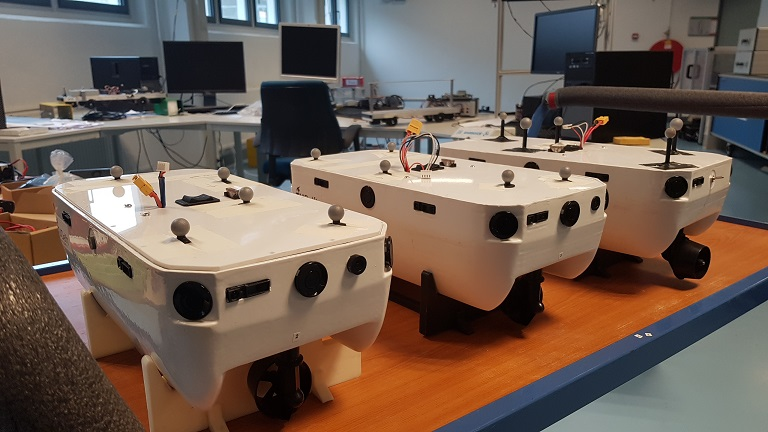
\includegraphics[width=0.9\textwidth]{20210414_121115}
	\caption{Delfia-* vessels, that will act as modules of the fleet system, to perform automated assembly and control.}
	\label{fig:DelfiaOverallLook}
\end{figure}

The approach of dividing a vessel control system via the Guidance, Navigation and Control categorization (\citet{fossen2011handbook} \& section \ref{analysisConfigAdaptation}) is used to distinguish between different system processes. However, the control for this particular system does refer to that of a single vessel, but rather to a set of vessels, which sometimes are controlled individually (when a module moves alone), and in other times together (in assembled platform). Hence, not only the system behavior changes (such as inertia of a platform of variable shape and size), but also the control structure. 


A control structure has been developed, working on three levels, depicted in figure \ref{fig:networkTopology1}. The concept of a 'platform' and a corresponding platform-controller are key to the functioning of this system.  Various tasks of the system are divided across agents that can be roughly described as follows:

\begin{itemize}
	\item A fleet manager
	\item A platform manager
	\item A module
\end{itemize}

\begin{figure}[h]
	\centering
	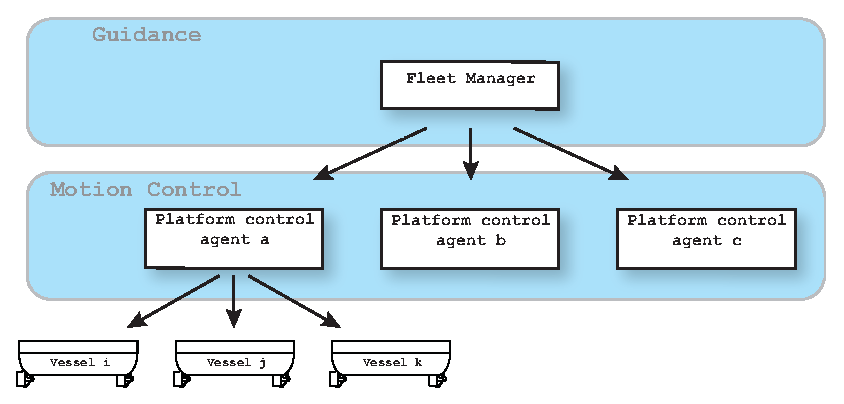
\includegraphics[width=0.9\textwidth]{networkTopology1V2}
	\caption{Hierarchical topology of the network. A single agent manages various platforms control agents. Platform control agents each manage a unique set of modules.}
	\label{fig:networkTopology1}
\end{figure}

A single fleet manager performs vessel guidance and coordination of the assembly process. These tasks are designed to operate as a rather simplistic state machine that runs trough phases based on system triggers or operator input. 

Tasks generated by the fleet manager are passed onto a set of Platform-controllers, which manage motion control of a set of connected modules in a centralized fashion. For every platform, a single agent is responsible for making decisions for all modules in the platform. This platform controller uses a reference state and a platform-state estimation to generate actuator responses for all modules. These are sent to the corresponding modules that make up the platform, which are then interpreted and executed. The platform controlling agent can be embodied by a computer anywhere on the network, given that it has sufficient computational power and the network is stable and reliable. 

The amount of modules that an platform-control-agent manages varies over time as vessels attach or disconnect. Thus all functions of the platform controller needs to be able to handle a variable amount of modules and configured shape. 

Communication between agents is facilitated by WiFi and the Robotic Operating System (ROS) as middleware. ROS facilitates communication between agents in a multi-robot system in an interoperable and modular way. This is thanks to the publisher-subscriber approach, which allows a variable amount of agents to listen (subscribe) to a dedicated datastream (topic). Similarly, a variable amount of agents can send (publish) various datatypes to such topics. This middleware has several benefits, one of which is the ability to set up various topics that represent some system information, on which agents running on various operating systems can send and receive data. The publisher-subscriber approach allows agents to only be subscribed to topics which are relevant. Furthermore, ROS also has many standardized message formats, libraries, and a large and rapidly developing userbase that further enhances interoperability.

State estimation of modules is done by an on-shore optical tracking system. Each vessel has a dedicated topic on which these estimates are published, which are accessible for all entities within the network by subscribing to that particular topic. 

The fleet manager has, besides creating references for the platforms, also the task of coordinating module ownership. As (dis)assembly criteria are met, platform controllers exchange ownership of a module. This informs a platform-controller that a module is connected, and that it now has access to utilizing that module's actuators. Figure \ref{fig:ownershiptransfer1} and \ref{fig:ownershiptransfer1} illustrate transfer of ownership of a module between two platform controllers, which can leave platform-controller-agents without modules under it's control, rendering it inactive. 
Each module will be controlled by a single platform-controller at a time. The platform controller will have full knowledge of the determined pose of each module in the platform with respect to the platform-coordinate system. 

 \begin{figure}[H]
	\centering
	\makebox[\textwidth][c]{
		\begin{minipage}{0.45\textwidth}
			\centering
			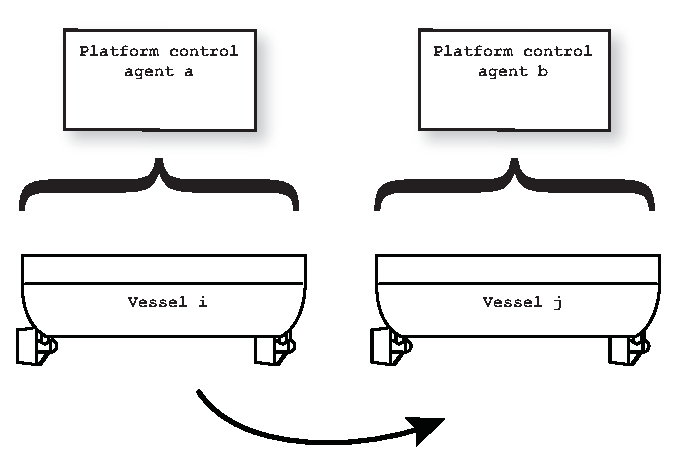
\includegraphics[width=0.95\textwidth]{img/controlAgent_separate}
			\caption{Two vessels that are both controlled by a separate control agent. A change in control structure can transfer module ownership (arrow).}
			\label{fig:ownershiptransfer1}
		\end{minipage}\hfill
		\begin{minipage}{0.45\textwidth}
			\centering
			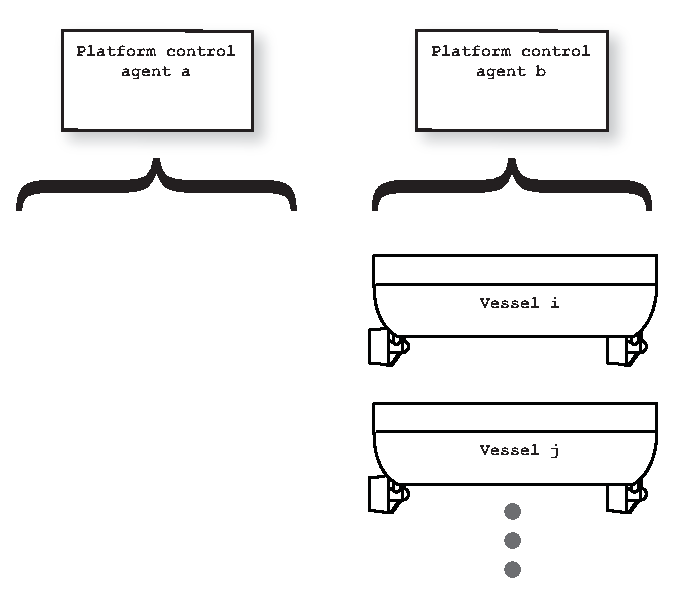
\includegraphics[width=0.95\textwidth]{img/controlAgent_together}
			\caption{Two vessels that formed into a platform, after which they are both controlled by the same agent.}
			\label{fig:ownershiptransfer2}
		\end{minipage}
	}
\end{figure}

\subsection{Platform Level Control Approach}
\label{subsection:PlatformControlApproach}
The platform controller has the goal of generating and publishing actuator commands for connected modules such that the platform motion follows the reference given by the fleet manager. 
The combined structure formed by the assembling modules will have a changing size and shape . This results in variable platform dynamics and number of available actuators. The overall approach on controlling the platform is illustrated in figure \ref{fig:motionControlApproach}. 
As modules connect or disconnect, the platform controller forms a model of the structure in the new configuration. The approach for estimating this model is elaborated in section \ref{platformModel}. Motion control is based on state feedback, where control effort generation and allocation are separated. The control effort generation block uses the estimated model to adapt actuator behavior to maintain performance while the system dynamics change. 
This control approach considers planar motion in 3-DOF (x, y, and yaw), neglecting pitch, heave and roll. 

\begin{figure}[H]
	\centering
	\captionsetup{justification=centering}
	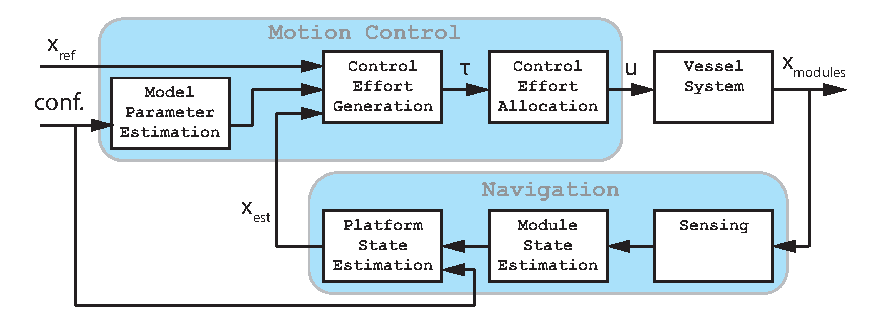
\includegraphics[width=150mm]{MotionControlAndNavigationLoopV3}
	\caption{The designed platform-motion control loop. State reference $X_{ref}$ is the main input from the Fleet manager (guidance system) and output is vessel state $X$. Occasional changes to configuration are communicated to the platform motion controller for adapting control strategy.}
	\label{fig:motionControlApproach}
\end{figure}

The goal is to find actuator commands for all modules under command of the controller such that the platform state approaches a reference state given by the fleet manager. The reference state will be a position and heading, noted as

\begin{equation}
X_{ref} = \eta_{ref} = \begin{bmatrix} x_{ref}\\ y_{ref} \\ \Psi_{ref} \end{bmatrix}
\label{eqPlatformControlRef}
\end{equation}
which is expressed in $\{n\}$. Note that other approaches might also include velocities as a state that is to be controlled, making the reference, estimated and actual state $X$ a [1x6] vector for motion in the surface plane instead of the [1x3] description as shown in equation \ref{eqPlatformControlRef}.

The control problem is solved in the following steps
\begin{itemize}
	\item An approximate model of the combined body is formed. Control gains are adjusted to estimated model parameters. 
	\item Platform state is estimated
	\item From this model, reference state and estimated state - control efforts are generated by means of a proportional-integrator-derivative (PID) controller.
	\item Control efforts are allocated between actuators on the modules. 
\end{itemize}

The state of the platform is defined as the origin and orientation of platform-body-fixed coordinate system $\{p\}$, expressed as 

\begin{equation}
\eta_{p/n}^{n} = \begin{bmatrix} x_{p/n}^{n}\\ y_{p/n}^{n} \\ \Psi_{p/n}^{n} \end{bmatrix}
\end{equation}

which is expressed in $\{n\}$. Note that platform origin is not defined to coincide with the centre of gravity. Connection of a module to the platform is considered binary, meaning a module would be either connected or disconnected, and cannot be 'connected a little'. Any change in platform configuration would result in an instantaneous displacement of the centre of gravity. As continuity of estimated state is desirable, the use of the centre of gravity was avoided to use as the definition of $\{p\}$.




\subsection{State Estimation}
\label{sec:stateEstimationDesign}

%From a set of sensors (on ships or shore) an estimation of the 'platform state' needs to be made. From this, and information of the modules that make up the platform
The platform state is but a concept to represent a collection of modules and is thus not directly measurable. It is however estimated by using a feedback signal of module positions and their known, constant placement within the body. Signal from a separate system performing state estimation of modules is translated to yield platform state estimates. Module localization can be done on board, on shore and with a variety of sensor systems, yet only needs to be consistently communicated on the robot network. Consider an update of the position and orientation of a module as
\begin{equation}
\eta_{b/n}^{n} = \begin{bmatrix} \textbf{p}_{b/n}^{n} \\[10pt] \Psi_{b/n}\end{bmatrix} = \begin{bmatrix} \textbf{x}_{b/n}^{n} \\[10pt] \textbf{y}_{b/n}^{n} \\[10pt] \Psi_{b/n}\end{bmatrix} 
\end{equation}

The known position of modules with respect to platform coordinate system as described by equation \ref{eq:moduleStaticPlacementEtaDefinition} is used to transform module to platform pose by subsequent rotation and translation. For the three considered degrees of surface plane motion the platform state becomes

\begin{equation}
\eta_{p/n}^{n} = \begin{bmatrix} \textbf{p}_{p/n}^{n} \\[10pt] \Psi_{p/n}\end{bmatrix}
\end{equation}
where
\begin{equation}
 \Psi_{p/n} = \Psi_{b/n} - \Psi_{b/p}
\end{equation}
and
\begin{equation}
\textbf{p}_{p/n}^{n} =  \textbf{p}_{b/n}^{n} - \textbf{p}_{b/p}^{n} =  \textbf{p}_{b/n}^{n} - \textbf{R}(\Psi_{p/n}) \textbf{p}_{b/p}^{p} 
\end{equation}


\subsection{Control Effort Generation}
\label{controlEffortGenerationDesign}
The control block is based on a Proportional-Integrator-Differential (PID) controller, designed to scale to model parameters which are estimated as described in section \ref{platformModel}. Three parralel controllers are used to control each individual degree of freedom, as illustrated in \ref{fig:parralelControl1}

\begin{figure}[H]
	\centering
	\captionsetup{justification=centering}
	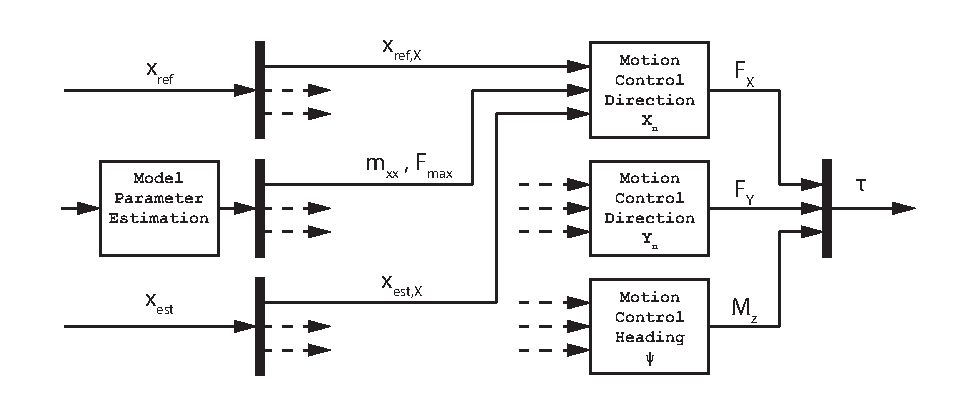
\includegraphics[width=0.9\textwidth]{parralelControl1}
	\caption{Parralel controller setup}
	\label{fig:parralelControl1}
\end{figure}

Control gains of the control-effort-generation block are designed to scale such that, once tuned for a single configuration, show similar behavior for any other configuration or platform size. For this, the following configuration dependent parameters are used. \\

\begin{itemize}
	\item Position of the centre of gravity
	\item Linear inertia, or mass
	\item Angular inertia
	\item Maximum available control effort for translation (maximum force)
	\item Maximum available control effort for rotation (maximum torque)
\end{itemize}

The centre of mass of the platform is found using equation \ref{eq:centreOfMassFindR}. It can then be substituted in equation \ref{eq:translatedToPlatformCentreOfMAss2} to express the equations of motion in that particular point. For three degrees of freedom in the surface plane this becomes shaped as

\begin{equation}
	\textbf{M}_{p}^{CG} = \begin{bmatrix}
	m_{xx} 	&	m_{xy}	& 0 		\\[10pt]
	m_{yx} 	&	m_{yy}	& 0 		\\[10pt]
	0 		&	0		& I_{zz} 	\\[10pt]
	\end{bmatrix}
\end{equation}
where

\begin{table}[H]
	\centering
	\begin{tabular}{ll}
		
		$	\textbf{M}_{11} = \begin{bmatrix}
		m_{xx} 	&	m_{xy}	\\[10pt]
		m_{yx} 	&	m_{yy}	\\[10pt] \end{bmatrix}$ & 
		
		$	\textbf{M}_{12} = \begin{bmatrix}	 0 	\\[10pt]  0	\end{bmatrix}$ \\[25pt]
		
		$	\textbf{M}_{12} = \begin{bmatrix}		0 	& 0 \end{bmatrix}$ &
		
		$	\textbf{M}_{22} =  I_{zz} $
	\end{tabular}
\end{table}



Which shows the estimated moment of inertia $I_{zz}$ in the bottomright corner. If modules have hydrodynamic added mass being modelled as a constant, direction-dependent constant, the off-diagonal elements $m_{xy}$ and $m_{yx}$ may be nonzero. This can also result that masses in $xx$ and $ yy$ direction may be unequal, which can feel rather counter intuitive, as this is never the case with normal rigid body motion. The cause of this still originates from the origonal form of module inertia matrix, as this inherited by using such models. 

The controllers responsible for linear motion will use an estimation of the mass of the platform. Rotating the inertial matrix can be done such that the off diagonal elements $m_{xy}$ and $m_{yx}$ become zero. The magnitude of the diagonal elements can be easily found, as they are the eigenvalues of $M_{11}$. The average of the eigenvalues is used as the estimated omni-directional mass for adapting controller behavior. For linear motion in 2 degrees of freedom (x and y) this becomes
\begin{equation}
	m_{p} \approx \frac{1}{2} \sum_{}^{}  Eig ( \textbf{M}_{11} )
\end{equation}

As the fleet utilizes rotatable azimuth thrusters, the maximum force is generated by the propellers on full power in a single direction. The maximum force that the platform can generate can be found by summation of maximum thruster force of all thrusters
\begin{equation}
\textbf{f}_{p,max} = \sum_{i=1}^{n_{thr}} f_{i,max}
\end{equation}
where $n_{thr}$ refers to the total amount of thrusters, and $f_{i,max}$ is the maximum force that the $i$th propeller can supply. The homogeneous fleet has two identical propellers per module, such that. 
\begin{equation}
\textbf{f}_{p,max} = 2*n* f_{prop,max}
\label{Maxforce1}
\end{equation}

Maximum torque is generated when all thrusters supply maximum force in the direction perpendicular to a vector between CG and the thruster. For a single vessel, this becomes
\begin{equation}
\textbf{m}_{i,max} = |\textbf{r}|  f_{i,max} =  | \textbf{p}_{CG/p}^{p} - \textbf{p}_{thr,i/p}^{p} |  f_{i,max}
\label{maxMoment1}
\end{equation}
where $ \textbf{p}_{CG/p}^{p} $ is the position vector of the platform $CG$ and $ \textbf{p}_{thr,i/p}^{p}$ is the position of the $i$th thruster. The latter is usually given in local frame of a module, but can be converted to platform coordinates by matrix rotation and a translation as:
\begin{equation}
\textbf{p}_{thr,i/p}^{p} =   \textbf{R}_{bj}^{p} \textbf{p}_{thr,i/bj}^{bj} + \textbf{p}_{bj/p}^{p}
\end{equation}
where $\textbf{p}_{thr,i/bj}^{bj}$ is the position of thruster $i$, mounted on module $j$, expressed in the body fixed coordinate system of module $j$. $\textbf{p}_{bj/p}^{p}$ is the position of module $j$ expressed in platform coordinate system. Summation of equation \ref{maxMoment1} over all modules yields total maximum torque generated by actuators for a given configuration as

\begin{equation}
\textbf{m}_{p,max} = \sum_{i=1}^{2n}  \textbf{m}_{i,max}
\label{maxmomentTotalSummed}
\end{equation}

It should be noted that the  equation \ref{Maxforce1} and \ref{maxmomentTotalSummed} show absolute maxima, which need full participation of all actuators to be reached. These maxima can not be obtained in different degrees of motion simultaneously, as outputs will be saturated. To avoid unpredictable control effort generation, actuator operation near output saturation is avoided during implementation.

The control blocks for each degree of freedom, as shown in figure \ref{fig:parralelControl1} operate based on PID control. Generic PID control starts by computing the state error by taking the difference between reference and state feedback. This error is fed parralel trough three different gains, where one signal is integrated and one is differentiated, until the signals are summed to yield the control output.

\begin{figure}[H]
	\centering
	\captionsetup{justification=centering}
	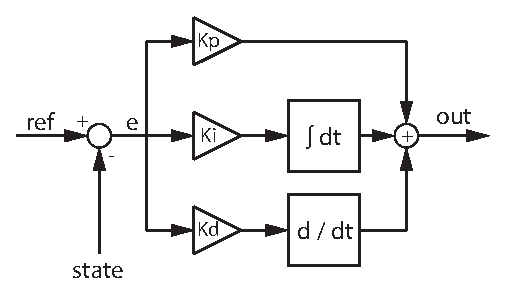
\includegraphics[width=0.4\textwidth]{simplePIDGeneric}
	\caption{A generic Proportional-Integral-Derivative control structure.}
	\label{fig:simplePIDGeneric}
\end{figure}

The control gains of the three parralel PID controllers are tuned to a single reference configuration. As the configuration changes the control gains will adapt to the newly estimated dynamics. 
The control gain scaling is based on the assumption that a configuration will have a response comparable to the reference, but in a different time scale. Typical errors that are fed into PID gains will thus be of comparable magnitude. System responses of current and reference configurations are thus aimed to be approximately comparable such that
\begin{equation}
	\eta_{c}(t) \approx \eta_{ref}(C*t)
	\label{eq:timescaling}
\end{equation}


 If control forces are a dominant factor to the response time of a step input on the system, a characteristic accelleration of a configuration can be defined as
\begin{equation}
a = \frac{Force}{Inertia}
\end{equation}

This is used to estimate the time scaling factor is estimated as the ratio of maximum accelleration of a configuration with respect to the reference configuration. 
\begin{equation}
C_{c} = \frac{a_{c}}{a_{ref}} = \frac{F_{c} \; I_{ref}}{F_{ref} \; I_{c}}
\label{eq:timescaleDef}
\end{equation}
where $ a_{c}$ and $a_{ref}$ are the characteristic accellerations of the current and reference configuration respectively. 

All gains is designed to scale to the maximum obtainable control effort. The base value of contribution is determined in the gain tuning process of the reference configuration. The eventual output of any proportional integral and derivative gains is multiplied by the maximum control effort in that dimention. 

Output of the control effort from proportional gain scales to the magnitude of the error, which assumed comparable in all configurations.  This could result in, for example, a proportional gain that is to contribute 60\% of the maximum obtainable control effort at an error of $e = 1.0$. The gain would become 
\begin{equation}
	K_{p} = K_{p,base}* \tau_{max} =  0.6* \tau_{max}
\end{equation}
such that the control effort contributed by the proportional block becomes
\begin{equation}
	\tau_{i,prop} = e * K_{p} = 0.6* \tau_{max}
\end{equation}

Integral control is however affected by the time in which the system responds. A system that responds slower ( $C_{c} < 1$ ) than the reference configuration will encounter additional integrator buildup. Time factor $C_{c}$ compensates for change of integrator output due to response time by adjusting integral gain as
\begin{equation}
	K_{i} = C_{c} \; K_{p,base} \; \tau_{max}	
\end{equation} 
such that integral control output becomes
\begin{equation}
\tau_{i,int} =  K_{i} \int_{0}^{t} e \; dt =  C_{c} \; K_{p,base} \; \tau_{max} \int_{0}^{t} e dt
\end{equation}

Derivative control output is also affected by time, but scales inversely to time factor $C_{c}$ with respect to integral control. Imagine, for example, a mass (*cough* *cough* vessel) that approaches the reference state, which would make the time derivative of the error negative. Derivative control would attempt to slow the mass down as it approaches it's desired state to avoid overshoot. An object, such as a container vessel, with low maximum control forces relative to the large mass would have to use take this speed more serious than highly manouverable vessels. Derivative adapts to a configuration as
\begin{equation}
K_{i} = \frac{K_{d,base} \; \tau_{max}}{C_{c}}	
\end{equation} 

Base values of controller gains ( $K_{p,base}$ ,$K_{i,base}$ ,$K_{b,base}$ ) will be set while revieuwing responses of the system in reference configuration. A PID controller can be manually tuned, or with the help of many tools such as automated PID tuning software. Linear motion in $x$ and $y$ direction will have identical control settings, as dependency on the orientation of reference frame $\{n\}$ is considered undesirable. 

\subsection{Control Effort Allocation}
\label{controlEffortAllocationDesign}
Control effort, as shown in the previous section, needs to be allocated onto the platform's actuators. The amount of thrusters available varies per configuration. Also placement and orientation of actuators can differ. 
A platform needs to be able to sufficiently control it's motion in all reasonably forseeable configurations. As the amount of different configurations is rather large, a general solution is used, that can solve the control effort allocation problem for all possible configurations. 
The designed control effort allocation protocol relies on the following main principle:
"The contribution of an actuator to a desired resulting force or moment is proportional to   its ability to contribute relative to that of the combined set of actuators."

This principle manifests particularly in rotational motion, as the ability of a thruster to generate torque relies on its placement with respect to the centre of gravity. Linear motion turns out not to exhibit such dependencies, as all thrusters are equal in strength, and possible orientation.  To compute actuator commands that satisfy the desired control effort,
it is allocated in each degree of freedom individually and finally combined.

Position of a thruster with respect to $CG$ can be expressed in $\{p\}$ by
\begin{equation}
\begin{split}
\textbf{p}_{t/CG}^{p} = \textbf{p}_{t/b}^{p} + \textbf{p}_{b/p}^{p} - \textbf{p}_{CG/p}^{p} \\
= \textbf{R}_{b}^{p} \textbf{p}_{t/b}^{p} + \textbf{p}_{b/p}^{p} - \textbf{p}_{CG/p}^{p}
\end{split}
\end{equation}

Thruster force vector can be expressed in $\{p\}$ in 3 degrees of freedom as
\begin{equation}
\begin{split}
\textbf{f}_{t}^{p} = \textbf{R}_{b}^{p} \textbf{f}_{t}^{p}
\end{split}
\end{equation}

The total resultant control effort from all modules in the centre of mass can be found by
\begin{equation}
m_{CG} = \sum_{i =1}^{n_{thrusters}} \textbf{p}_{ti/cg} \times \textbf{f}_{ti}
\label{torqueCG1}
\end{equation}
\begin{equation}
f_{CG} = \sum_{i =1}^{n_{thrusters}}  \textbf{f}_{ti}
\end{equation}
or in vector form as
\begin{equation}
\tau_{CG} = \sum_{i =1}^{n_{thrusters}}  \textbf{H}^{\top}(\textbf{p}_{t/CG}^{p}) \begin{bmatrix}
\textbf{f}_{ti}^{p} \\ 0_{1x3}
\end{bmatrix}
\end{equation}
where $\textbf{p}_{ti/CG}$ is the position of the $i$th thruster with respect to the platform's centre of gravity, and $\textbf{f}_{ti}$ refers to the force vector applied by the $i$th thruster.
Where it should be noticed that the zeros represent torque applied by the propeller, as propellers are modelled as a forcevector applied in a point. A resulting moment can be created due to the fact that thrusters are placed at a distance from $CG$.


The approach on generating control effort that results into torque is as follows. A force at a distance from $CG$ creates a higher resulting torque. The linear relation between torque and distance between applied point and $CG$ can be seen in equation \ref{torqueCG1}. Only considering forces in the $xy$ plane gives
\begin{equation}
	m_{zz} = x_{ti/CG} \; f_{y}  \; -  y_{ti/CG} \; f_{x}
	\label{mzz3dof}
\end{equation}
So at a constant force, the generated moment proportionally increases with distance. For a single direction ($x$ or $y$) this would be shaped as shown in figure \ref{fig:rampThrust}. Thruster contibution to torque that is to be deployed proportional to the effectiveness of the thruster results in a quadratic shape. Figure \ref{fig:paraThrust} shows how the quadratic contribution of a thruster at varying distance

\begin{figure}[H]
	\centering
	\makebox[\textwidth][c]{
		\begin{minipage}{0.45\textwidth}
			\centering
			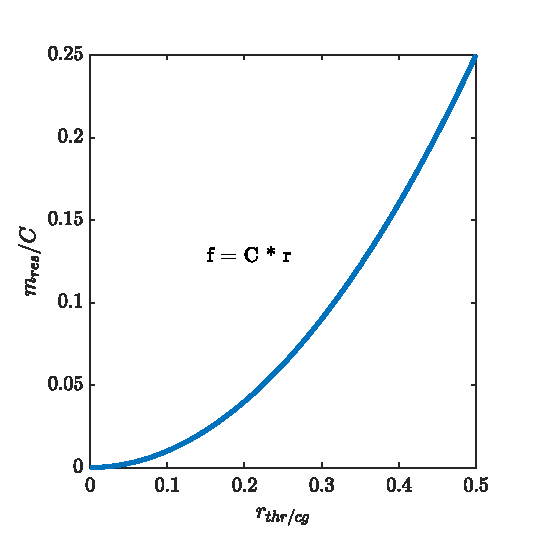
\includegraphics[width=0.95\textwidth]{ThrustAllocPara}
			\caption{Linear relation between resulting moment and thruster distance from $CG$, while thruster force is constant}
			\label{fig:rampThrust}
		\end{minipage}\hfill
		\begin{minipage}{0.45\textwidth}
			\centering
			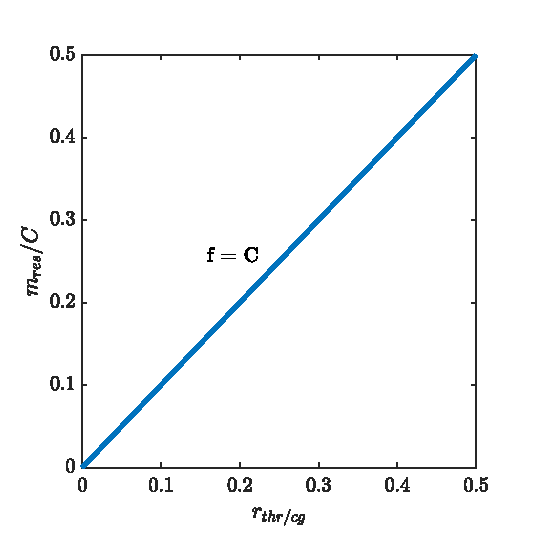
\includegraphics[width=0.95\textwidth]{ThrustAllocLin}
			\caption{Quadratic relation between resulting moment and thruster distance from $CG$, due to a thruster force being controlled to be proportional to distance}
			\label{fig:paraThrust}
		\end{minipage}
	}
\end{figure}

Thruster force to contribute to realizing a desired resulting moment is set as
\begin{equation}
	f_{x} = C_{m} \; m_{d} \; (- y_{ti/CG})
	\label{fx1}
\end{equation}
\begin{equation}
	f_{y} = C_{m} \; m_{d} \; x_{ti/CG}
	\label{fy1}
\end{equation}
where $C_{m}$ is a configuration dependent participation factor for torque and $m_{d}$ is the desired resulting moment of the combined structure. The resulting moment of a thruster becomes (by substituting \ref{fx1} and \ref{fy1} in \ref{mzz3dof})
\begin{equation}
m_{ti} = C_{m} \; m_{d} \; [ x{_{ti/CG}}^{2} \; + \; y{_{ti/CG}}^{2} ]
\end{equation}
The resulting moment of all thrusters satisfies
\begin{equation}
\begin{split}
m_{res} = m_{d} =  \sum_{i =1}^{n_{thrusters}} m_{ti} \\
= C_{m} \; m_{d} \; \sum_{i =1}^{n_{thrusters}}  \; [ x{_{ti/CG}}^{2} \; + \; y{_{ti/CG}}^{2} ]
\end{split}
\end{equation}
From which the total configuration dependent participation factor can be found, as
\begin{equation}
\begin{split}
C_{m} = \frac{1}{ \sum_{i =1}^{n_{thrusters}}  \; [ x{_{ti/CG}}^{2} \; + \; y{_{ti/CG}}^{2} ] }
\end{split}
\end{equation}
This constant ends up scaling all thruster contribution such that the overall relationship between thruster contribution and distance is quadratic, and that the resultant moment matches the desired moment. 


For linear motion a similar principle of contribution to effectiveness is applied, yet turns out much simpler. The homogeneous fleet has thrusters that are all equal in strength, and able to turn in all directions. As all thrusters are thus equally able to contribute to linear motion, total desired thrust is equally divided between all thrusters such that

\begin{equation}
f_{d} = \sum_{i=1}^{n_{thrusters}} * f_{ti}
\end{equation}

\begin{equation}
f_{ti} = C_{f} \; f_{d}\;  f_{max}
\end{equation}

\begin{equation}
C_{f} = \frac{1}{n_{thrusters}}
\end{equation}


All degrees of freedom that are affected by elements from the vector of desired control effort are evaluated independently, resulting in a forcevector for every thruster for every degree of freedom. The forcevectors pertaining to a thruster in all degrees of freedom are summed to obtain the overall contribution of that thruster. For three degrees of freedom this becomes
\begin{equation}
	\textbf{f}_{ti} = \textbf{f}_{ti,fx} + \textbf{f}_{ti,fy} + \textbf{f}_{ti,m}
\end{equation}
Fig. \ref{fig:controlAllocationSeparate1} illustrates how the control allocation problem is solved by combining actuator responses from elements of the desired control effort vector. 

\begin{figure}[H]
\centering
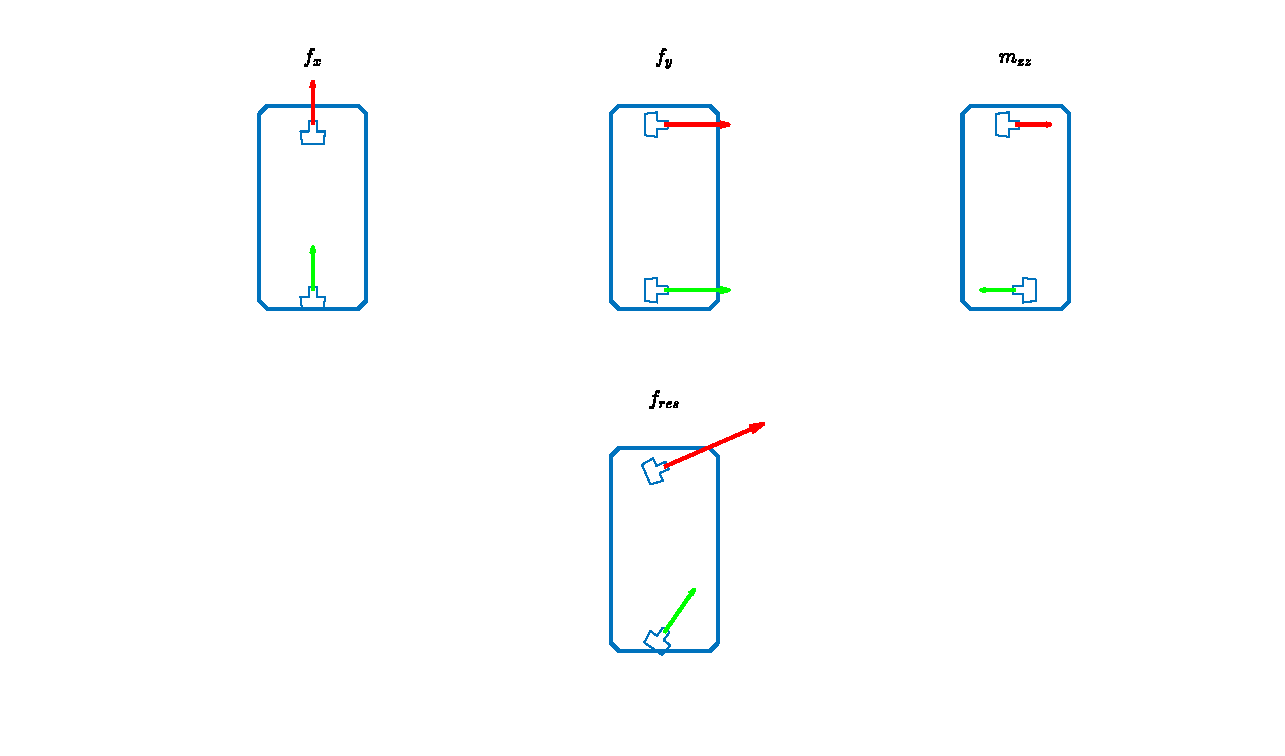
\includegraphics[width=\textwidth]{actuation_combined}
\caption{The approach of solving control allocation in each dimention separately, illustrated for a single vessel configuration. Three dimensions along which control effort is required are solved (above). The forces of the three solutions are combined to yield the final solution (below). }
\label{fig:controlAllocationSeparate1}
\end{figure}

\subsection{Assembly Protocol}
\label{assemblyProtocolDesign}
Modules will assemble in a lattice structure, using active magnets to remain configured. Task execution, including assembly, operates in a phasewise fashion. Generating the desired configuration (blueprint) and assembly planning are done by the operator for this project. 
The following steps are considered to achieve assembly of a module or platform to another:
\begin{itemize}
	\item The connecting object lines up with the assembly at a short distance, such that it can freely reach the connection site. During this process both objects are controlled by different controllers. 
	\item The connecting object moves to the connection site. Magnet connectors within area of acceptance of a connection site make contact, and connect. 
	\item Success of connectivity is evaluated before continuing
	\item If connected, ownership of the connecting bodies is transferred to the controller of the assembly. The other controller becomes inactive. (see figure \ref{fig:ownershiptransfer1} and \ref{fig:ownershiptransfer2})
	\item The controller of the assembly recomputes configuration dependent parameters on:
	\begin{itemize}
		\item The estimated platform model, as in section \ref{platformModel}
		\item The control effort generation protocol, by adapting controller gains to the newfound model estimate, as in section \ref{controlEffortGenerationDesign}
		\item   The control allocation protocol, to divide generated control effort over the new configuration as described in section \ref{controlEffortAllocationDesign}.
	\end{itemize}
	\item The assembly runs the adapted control scheme for further tasks.
\end{itemize}


\begin{figure}[H]
	\centering
	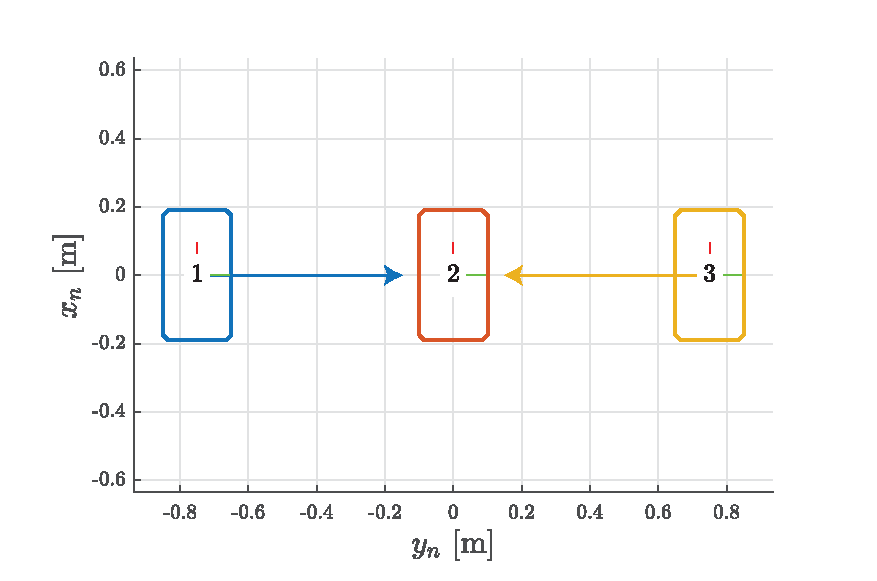
\includegraphics[width=0.7\textwidth]{matlabEvaluationFig14c}
	\caption{Platform assembly protocol from top vieuw. Vessel 1 and 3 are lined up to approach connecting to vessel 2 on either side. Once connectors are within range, the magnets snap into place, fixing relative motion.}
	\label{fig:matlabEvaluationFig14c}
\end{figure}


% The forces and moments represented by the acceleration hydrodynamic coefficients can, to a very great extent, be modeled as potential flow phenomena. Neglecting the details of the boundary layer in modeling acceleration-dependent forces and moments acting on a submerged body yields quite satisfactory results for most stability and control simulation. " \ref{humphreys1978prediction}


	
\section{Implementation} %Control Approach}
\label{chap:controlApproach}

The conceptual design elements that are explained in the previous section have been implemented to represent the envisioned framework. This section illustrates how designed concepts are realized in various hardware and software components. 

Physical system components are first introduced to shed light on the experimental facility, localization system and give more details on low level actuator control systems running on the modules. The multi-robot network setup is explained showing how various system components communicate. A object oriented Matlab software-framework been developed aimed to be reusable and intererable for other multi-vessel experiments within RAS. This framework, its structure, relation between classes, and means of implementing the designed control approach are explained in section \ref{sec:controlSoftware}.

Throughout developments many iterative changes were made to the system, of which two facets are discussed in section \ref{AdjustmentsAfterTests} starting with the process of tuning control gains and secondly an improvement of the assembly protocol using normal forces between modules to aid connectors reaching area of acceptance. 

Behaviors and responses of the system in development are occasionaly shown to support design choices. Behavior of the system in final stage of development is shown and evaluated in the next chapter. 

\subsection{System Components}
\label{imp:syscomponents}
The implemented control system consists of three key components
\begin{itemize}
	\item An optical tracking system for module localization.
	\item A computer that executes the control protocol and distributes generated tasks to the entire fleet.
	\item A set of Delfia-1* modules
\end{itemize}

This section provides details on the experimental setup of the optical tracking system and modules. Functionality of the control software is discussed in a separate section (\ref{sec:controlSoftware}). 

%\subsubsection{Experimental facility and Optical tracking system}
The experimental setup is designed to operate in the towing tank facility of section Maritime and Transport Technology (section MTT) in the faculty of Mechanical, Maritime and Materials Engineering (Faculty 3ME). One of such tanks is equipped with an optical sensing and interpretation system from the brand Optitrack. A 40 meter section of the tank is covered by cameras. Optitrack's motion capture software supports defining a set of infra-red reflectors as a rigid body. The camera setup was set up to interpret images to estimate state of the defined bodies (modules), and broadcast them on dedicated ROS topics at a frequency of 30hz. 

\begin{figure}[h!]
	\centering
	\captionsetup{justification=centering}
	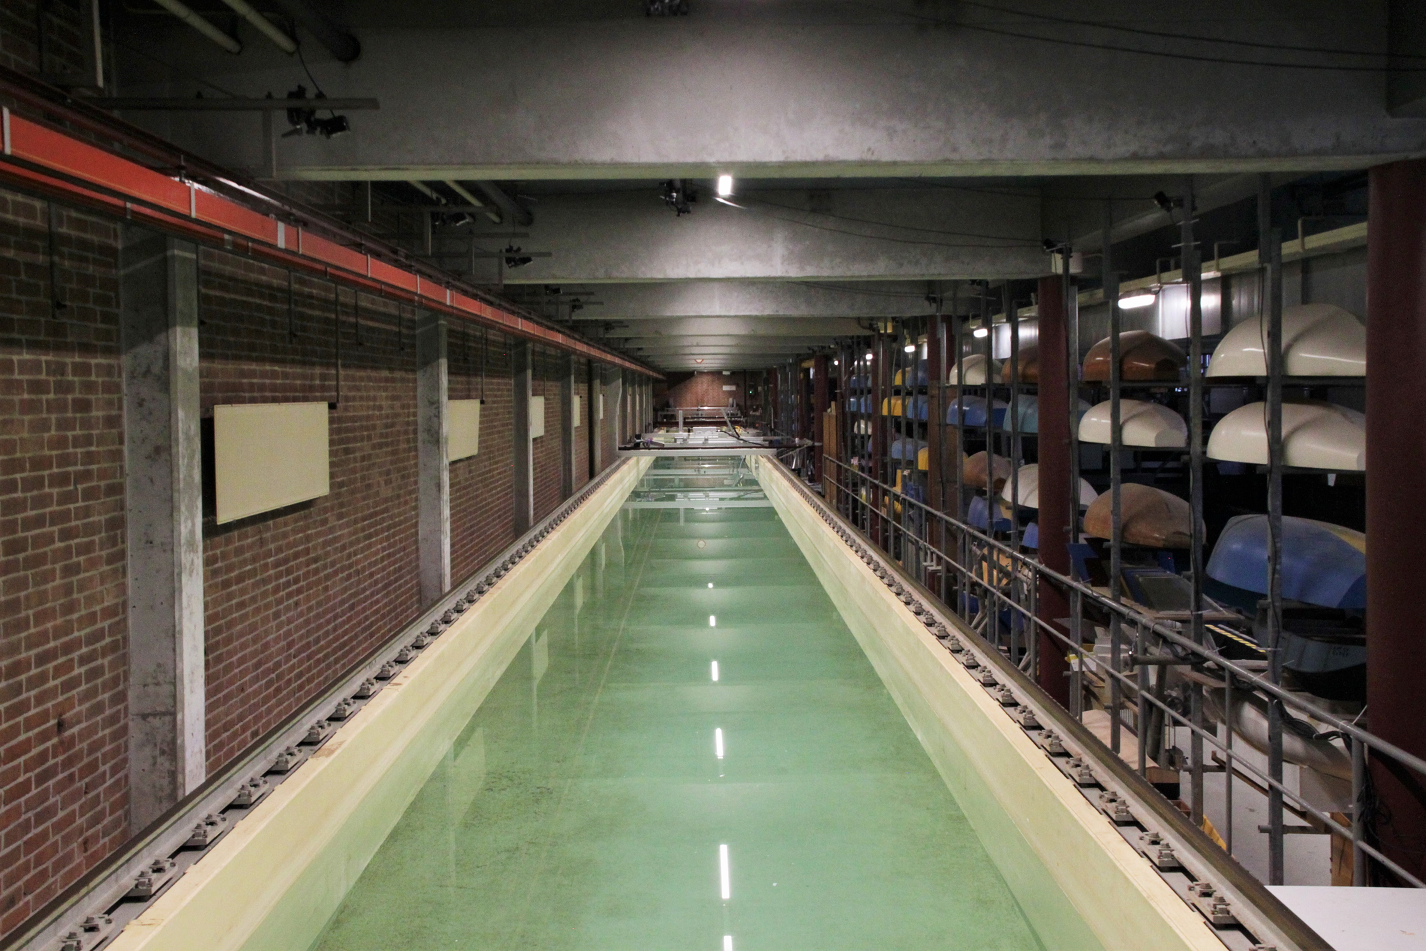
\includegraphics[width=0.9\textwidth]{img/IMG_4805b_downsized}
	\caption{The MTT towing tank facility at 3ME.}
\end{figure}


\begin{figure}[H]
	\centering
	\makebox[\textwidth][c]{
		\begin{minipage}{0.4\textwidth}
			\centering
			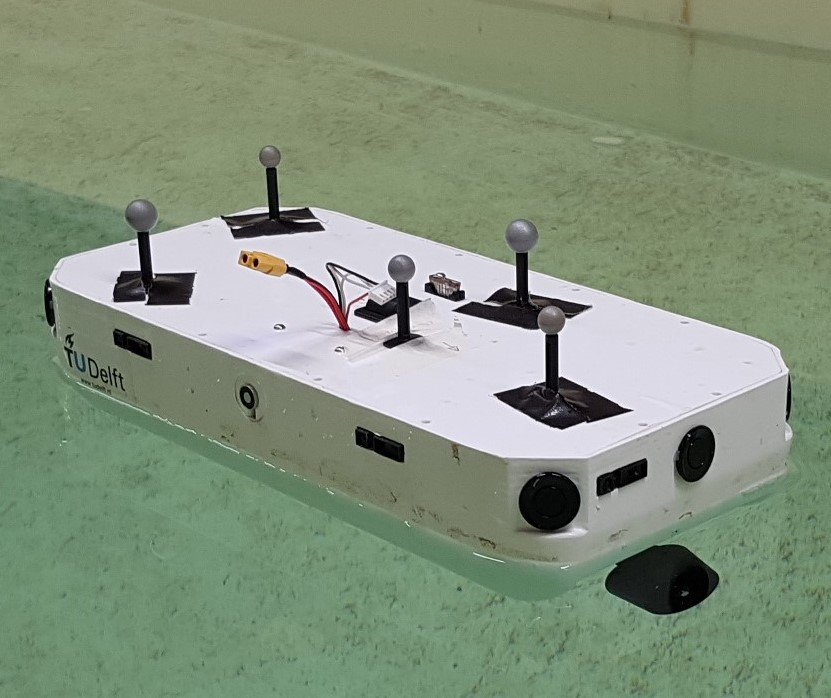
\includegraphics[width=0.95\textwidth]{img/singleDelfiaInfraRedTrackers}
			\caption{Five infra-red reflectors on top of a Delfia-1* module.}
		\end{minipage}\hfill
		\begin{minipage}{0.55\textwidth}
			\centering
			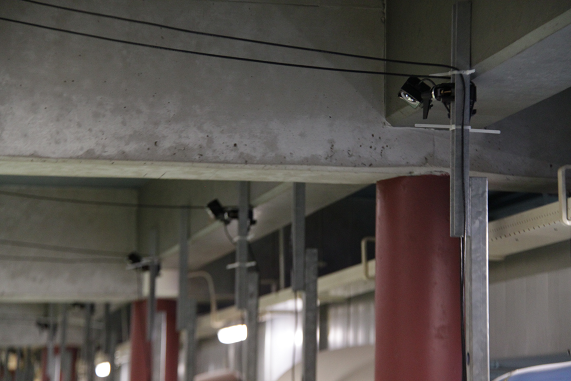
\includegraphics[width=0.95\textwidth]{img/IMG_4810_downsized}
			\caption{Motion tracking cameras mounted along the experimental setup.}
		\end{minipage}
	}
\end{figure}

\begin{figure}[H]
	\centering
	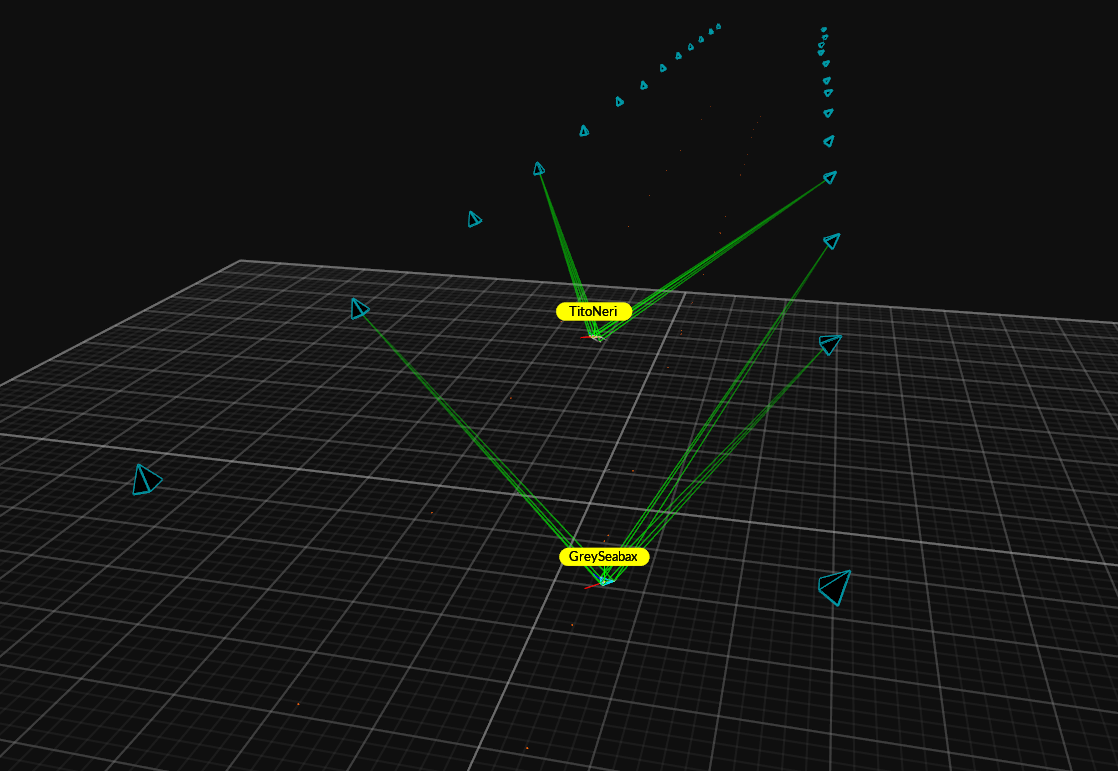
\includegraphics[width=0.7\textwidth]{OptitrackRays}
	\caption{Optitrack motion tracking with the towing tank setup, showing two deployed vessels. Green lines depict rays of reflectors that are succesfully being tracked}
\end{figure}


%\subsubsection{Delfia-1* Modules}
The Delfia-1* vessel (also refferd to as 'Delfia') is a model scale, electrically powered ship, equipped with two 360 degree rotatable azimuth thrusters. There are a total of four main actuators that are controlled by an on board system, referred to as the 'low-level control system'. The two azimuth thrusters are identical, and both have their orientation and propeller speed managed by a single microprocessor of the open-source Arduino project. Control of propeller speed and thruster angle is done with different hardware components, yet both rely on similar PID feedback control principles. Figure \ref{DelfiaDOF} illustrates the states that the low level control system needs to manage for one thruster. 

\begin{figure}[h!]
	\centering
	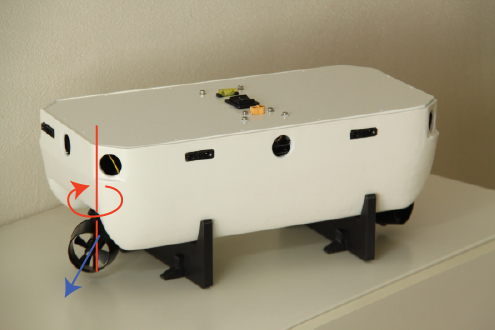
\includegraphics[width=0.7\textwidth]{IMG_4564}
	\caption{Degrees of freedom of one azimuth thruster. Each thruster (front and back) needs its direction (red) and propeller speed (blue) controlled.}
	\label{DelfiaDOF}
\end{figure}
All decisions for the low level control system are made on the on board microprocessor. This controller responds to actuator reference commands via USB serial port connection. Connectivity of the low level control system with other elements in the network is done through a Raspberry-Pi, as illustrated in figure \ref{delfiaConnectionNW}. The Raspberry-pi is the connecting element to the ROS network (via wifi) and the Arduino (via USB serial protocol). Other solutions exist that provide similar connectivity, yet a Raspberry-pi has some processing power which allows distribution of some, or all control tasks in future projects. 

\begin{figure}[H]
	\centering
	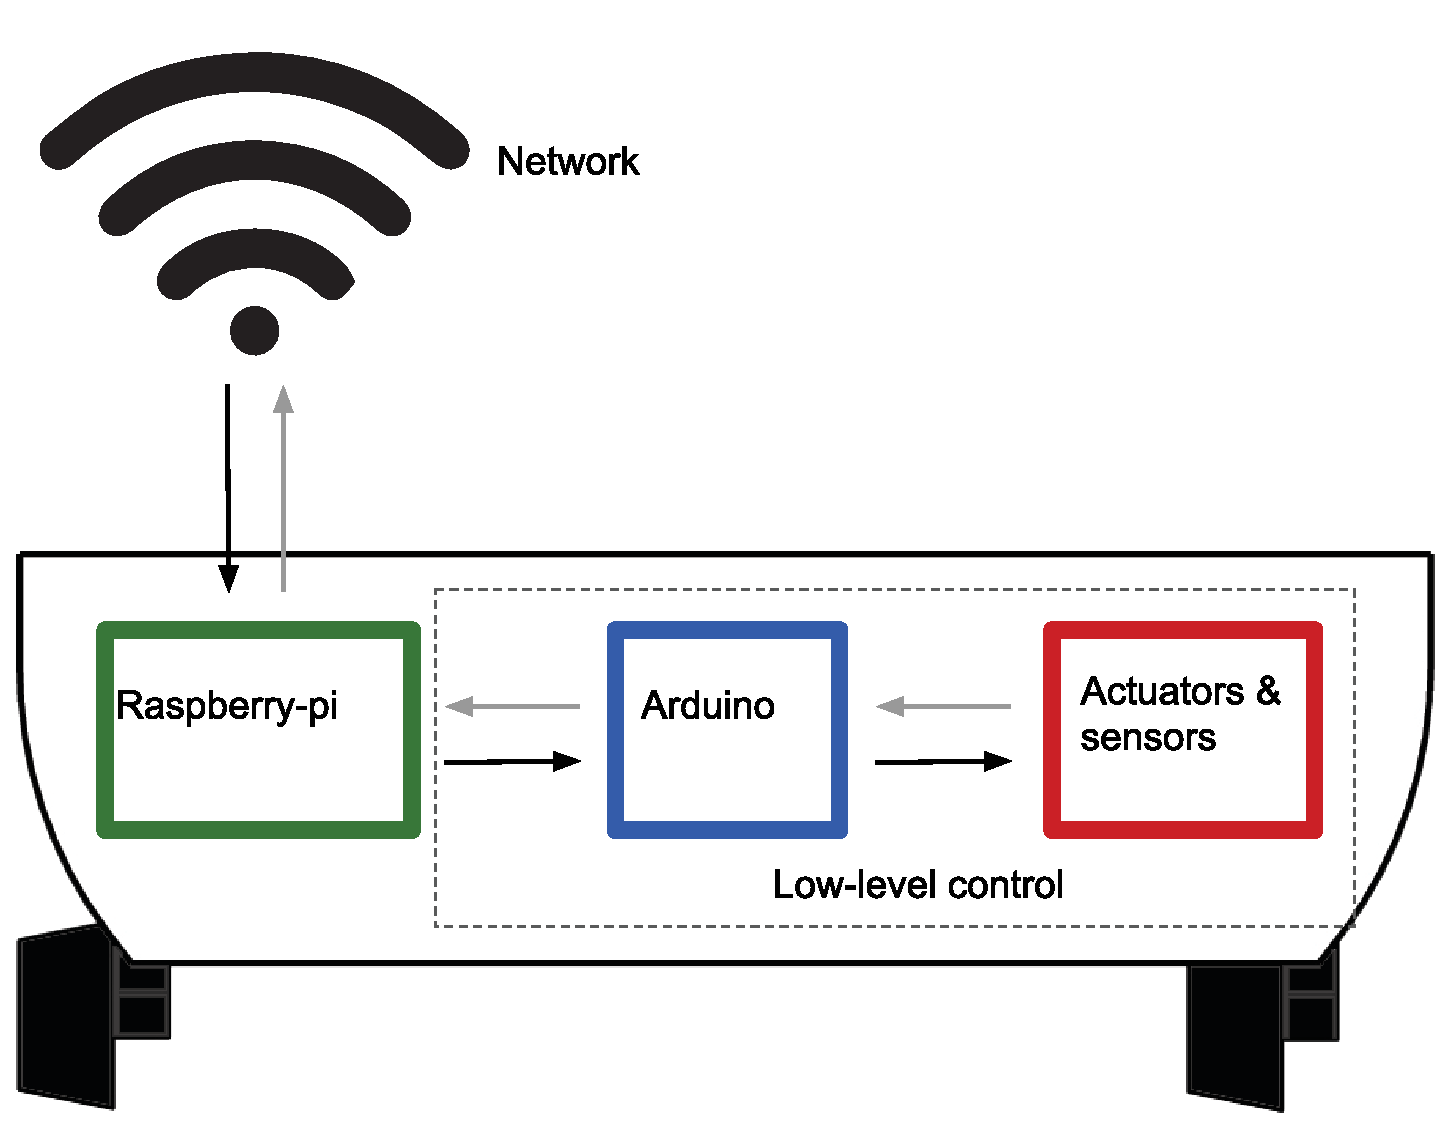
\includegraphics[width=0.5\textwidth]{DelfiaNetworkSchematicLowLvl1}
	\caption{The interaction of the Delfia's low level control system with on board computer (Raspberry-pi) and the vessel network.}
	\label{delfiaConnectionNW}
\end{figure}

The propeller is powered with an electrical 12V DC engine, while a sensor signal on speed is created by means of an optical encoder. Figure \ref{DelfiaDriveTrain} shows the propeller drivetrain that can be found above each thruster, and figure \ref{propellerFBLoop} illustrates the feedback loop that controls propeller velocity. 

 \begin{figure}[h!]
	\centering
	\makebox[\textwidth][c]{
		\begin{minipage}{0.45\textwidth}
			\centering
			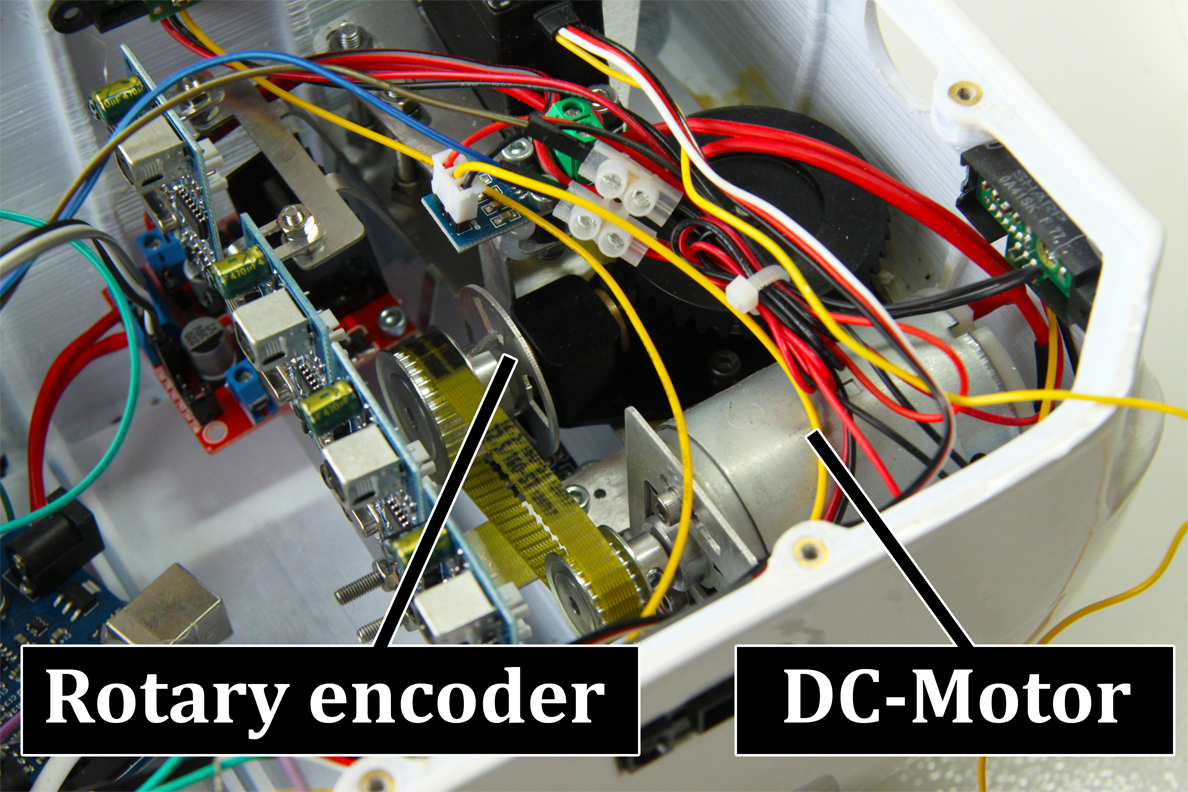
\includegraphics[width=0.95\textwidth]{img/delfiaDriveTrain_edited}
			\caption{The propeller drivetrain. The rotation in the axle of the DC-motor is transferred to the propeller via a belt and gears.}
			\label{DelfiaDriveTrain}
		\end{minipage}\hfill
		\begin{minipage}{0.45\textwidth}
			\centering
			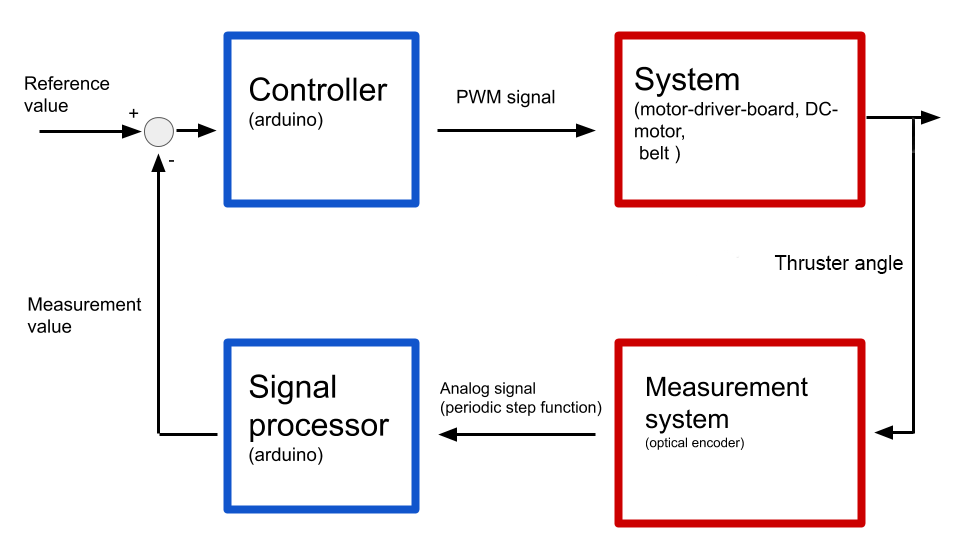
\includegraphics[width=1.1\textwidth]{img/propellerFBLoop}
			\caption{The feedback loop of the low level propeller-speed control system}
			\label{propellerFBLoop}
		\end{minipage}
	}
\end{figure}

Each thruster angle is actuated by a ''Parallax Feedback 360° High-Speed Servo''. Thruster and servo are connected via a rubber cog belt (figure \ref{DelfiaServoTrain}). The servo needs a 50Hz PWM signal as input and uses a hall effect sensor to provide angular position feedback as a 910Hz PWM signal. The feedback loop that controls the thruster angles is as shown in figure \ref{DelfiaServoLoop}.

 \begin{figure}[h!]
	\centering
	\makebox[\textwidth][c]{
		\begin{minipage}{0.45\textwidth}
			\centering
			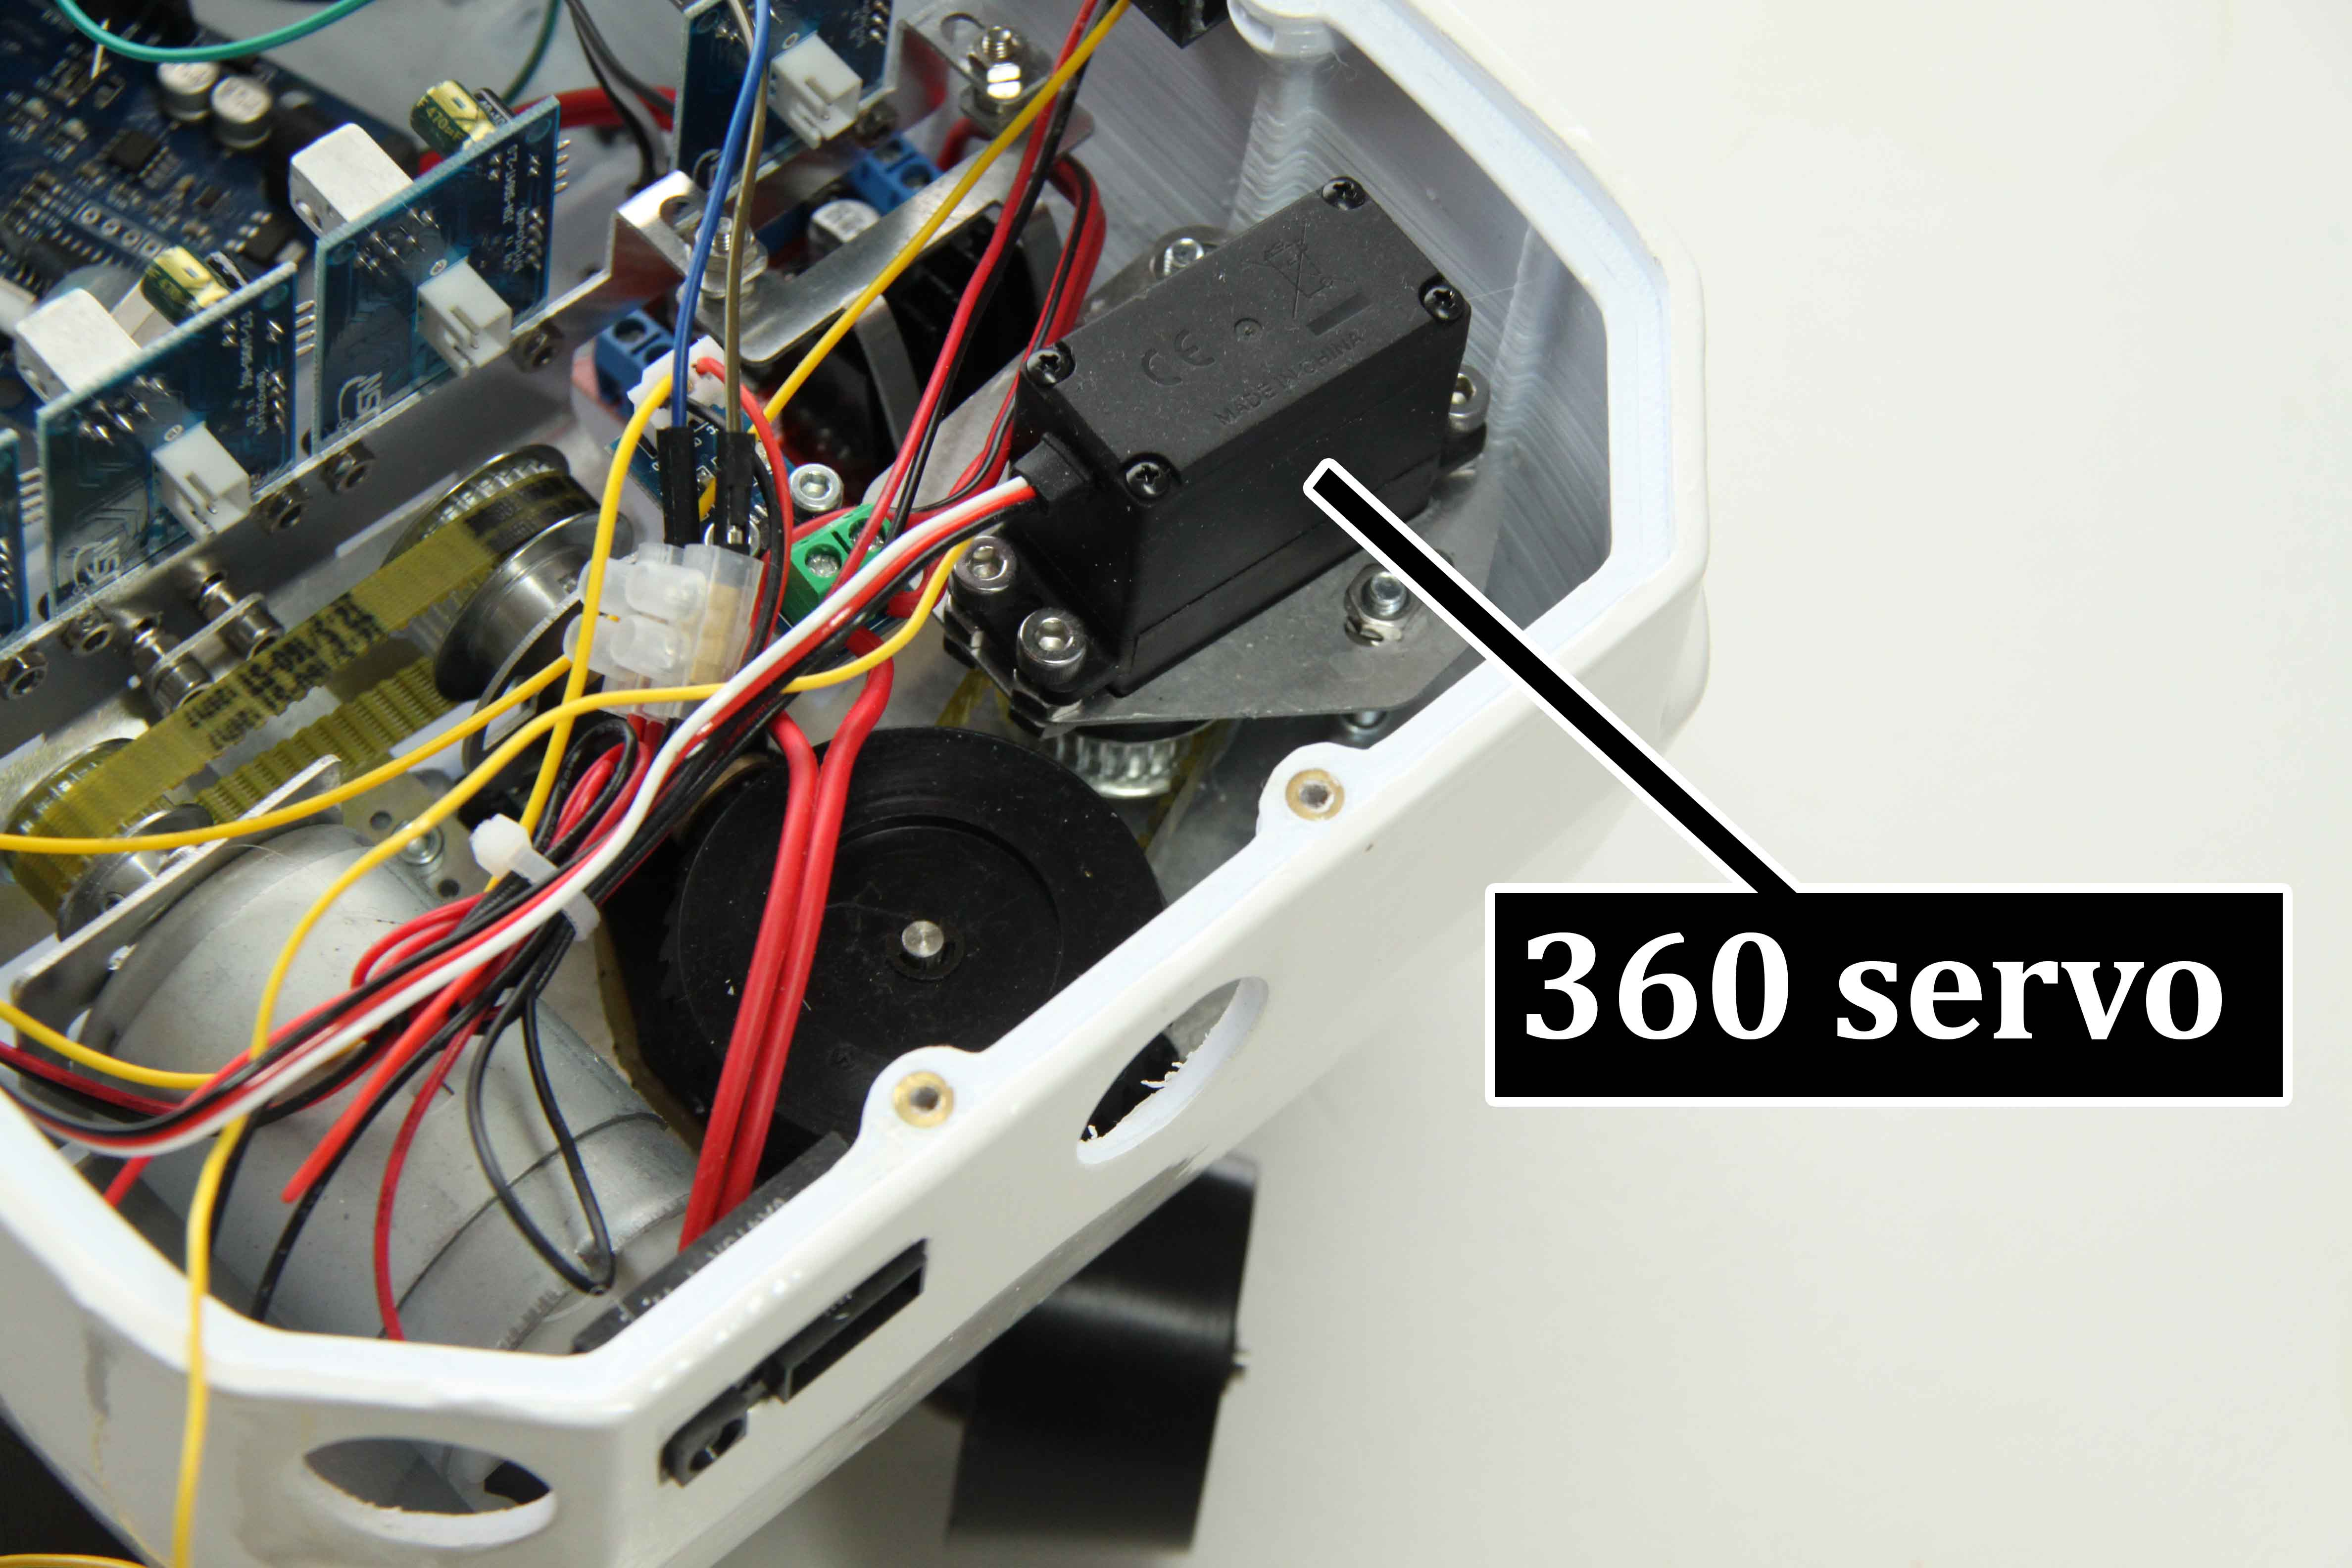
\includegraphics[width=0.95\textwidth]{img/delfiaServo_edited}
			\caption{The propeller drivetrain. The rotation in the axle of the DC-motor is transferred to the propeller via a belt and gears.}
			\label{DelfiaServoTrain}
		\end{minipage}\hfill
		\begin{minipage}{0.45\textwidth}
			\centering
			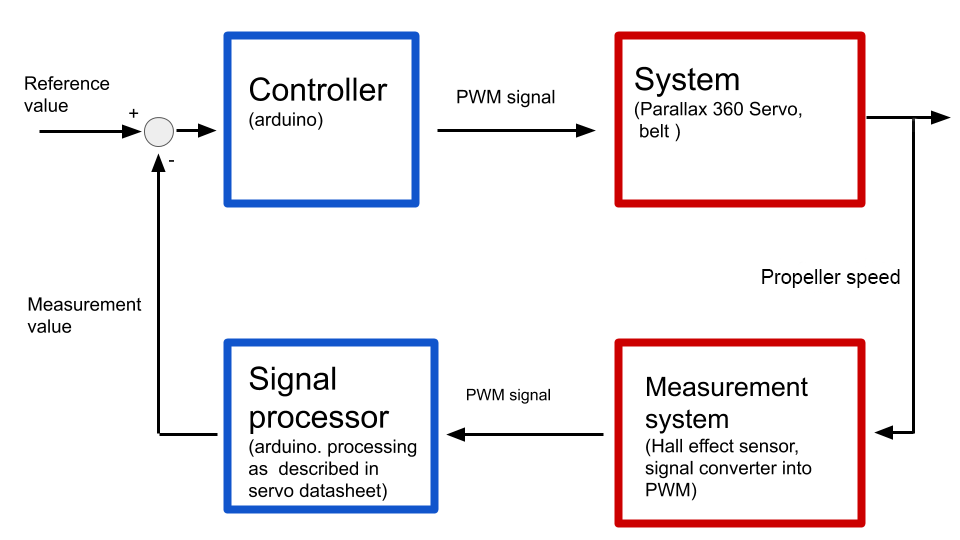
\includegraphics[width=1.1\textwidth]{img/servoFBLoop}
			\caption{The feedback loop of the low level thruster angle control system}
			\label{DelfiaServoLoop}
		\end{minipage}
	}
\end{figure}


Fundamentals of the Delfia-1* low level control system have been developed during a research project \citet{boogmans2020Delfia}, by the same author as this work. Development of hardware and software is described therein, and parameter tuning is done by means of evaluating reference step responses. Characteristic control system behavior is shown in figures \ref{delfiaLowStepProp1} and \ref{delfiaLowStepServ1} for propeller-speed and thruster-angle respectively. Note how the propeller speed signal contains significant fluctuations, of which the majority is considered sensor noise. An optimum trade-off point of signal filtering was found between smoothness and increased latency. High frequency notes in this signal (order of $10^3$hz) that translate to engine control effort will not result in noticable differences of vessel dynamics response, as the  vessel responds in much lower frequencies (order of $10^0$ hz). 

\begin{figure}[H]
	\centering
	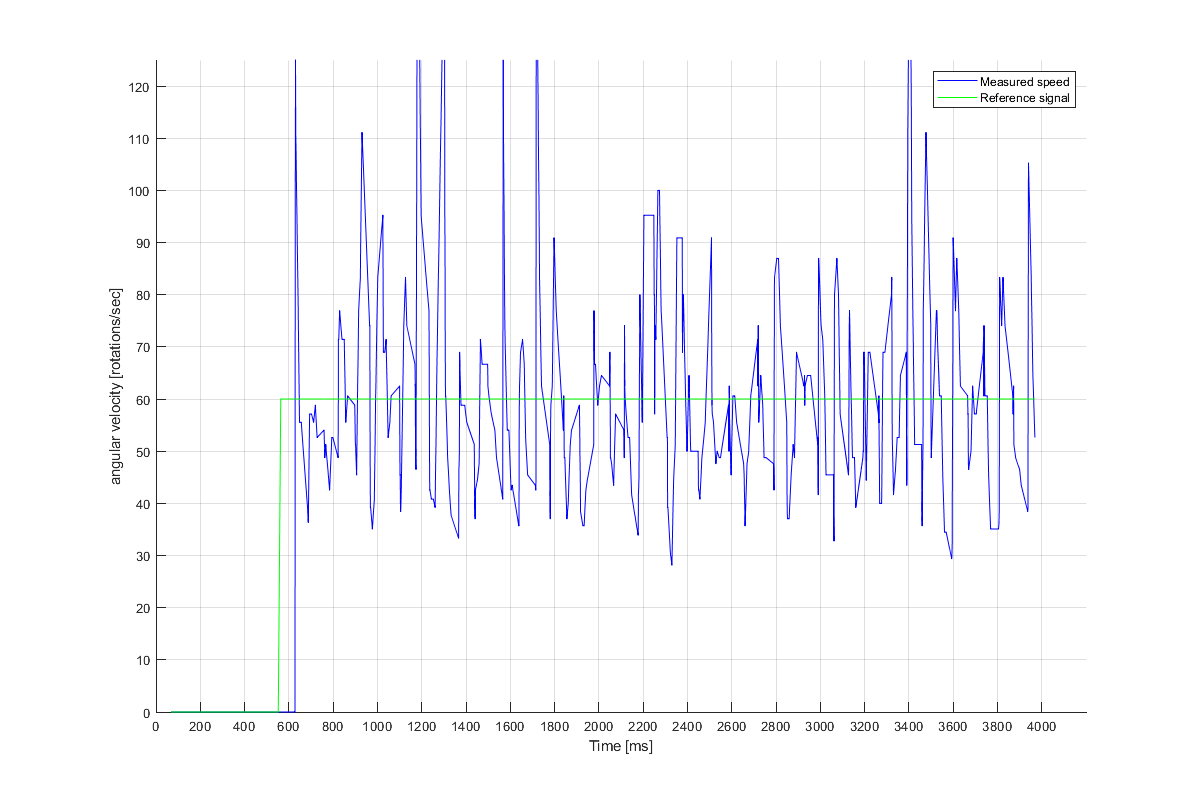
\includegraphics[width=0.85\textwidth]{img/4e-2_2e-2_0_130hz_n=8}
	\caption{Measured signal of a characteristic step-response of the propeller-speed control system. Considerable high frequency notes can be observed, although it oscillates rather well around the reference input.}
	\label{delfiaLowStepProp1}
\end{figure}

\begin{figure}[H]
	\centering
	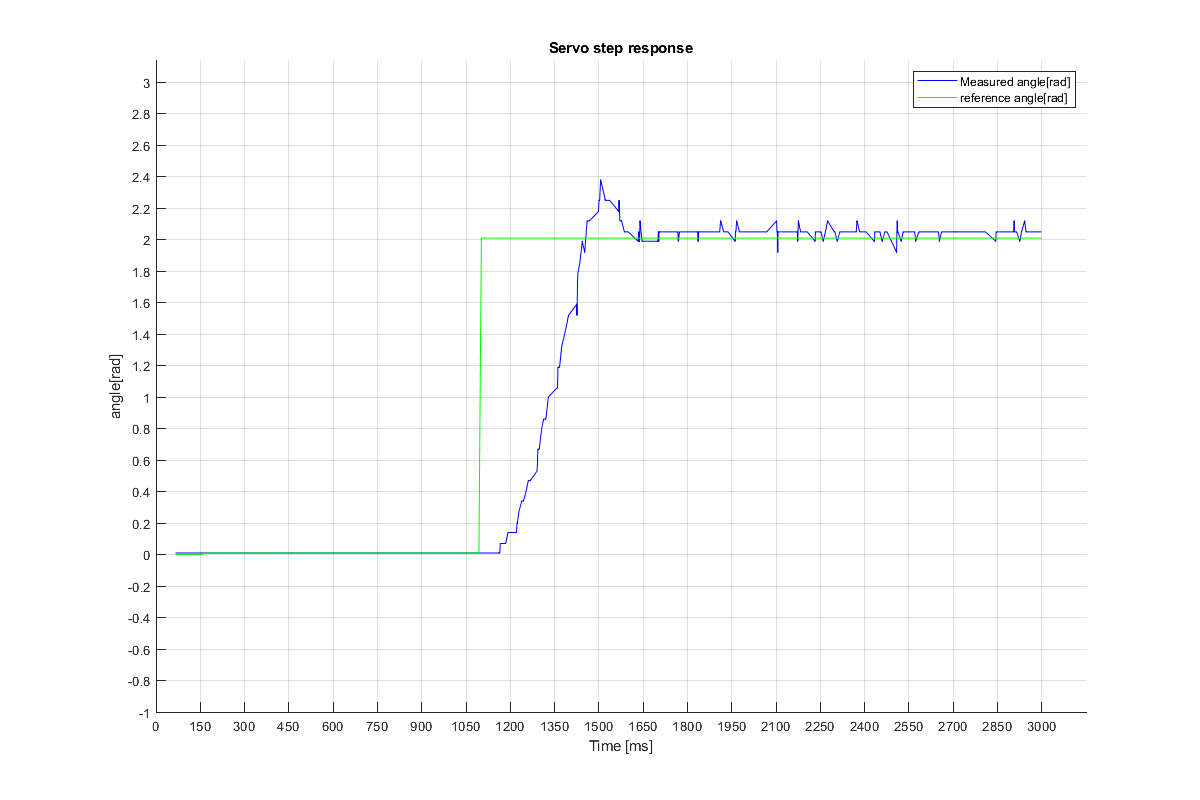
\includegraphics[width=0.85\textwidth]{img/Kp_1e0_Ki_8e-3_Kd_4}
	\caption{Measured signal of a characteristic step-response of the thruster-angle control system.}
	\label{delfiaLowStepServ1}
\end{figure}

It is worth noting that the slope of the servo step response, as shown in figure \ref{delfiaLowStepServ1}, proved quite consistent with more agressive controller gains. Higher proportional or integral gain caused more overshoot, or even instability, without the benefit of a quicker response time. This is considered simply due to the maximum rotation speed of the servo. 


Actuators that connect the modules have been developed and implemented as a set of active magnets, or solenoids, shown in figure \ref{fig:solenoidsMF} and \ref{fig:solenoids}. Models are available in various lifting capacities, and a $10N$ model that operates at $12V$ was estimated to provide enough force for vessels to remain connected in reasonably expected scenarios. It is powered by the $12V$ micro powergrid from the on-board battery.  Higher powered magnets draw more power, and this variant seemed a good balance at a $1.0W$ power consumption. Mounts for the connectors were developed and fabricated by a 3D printer to fit in existing slots in the Delfia's hull.

At first, connections were implemented where a connection was made between two vessels with connectors of opposite polarity. Magnet connector polarity can be reversed by reversing the potential on coil connectors. This can be automated with, for instance, an H-bridge. Tests proved connector force to be insufficient between connecting solenoids. Attracting forces to a piece of iron did give the desired results, thus connector counterparts were lathed to size. Available 3D printers proved to have tolerances sufficient such that connector parts, both magnet and piece of iron, were made to stay in the mouts by using a press. 


 \begin{figure}[H]
	\centering
	\makebox[\textwidth][c]{
		\begin{minipage}{0.48\textwidth}
			\centering
			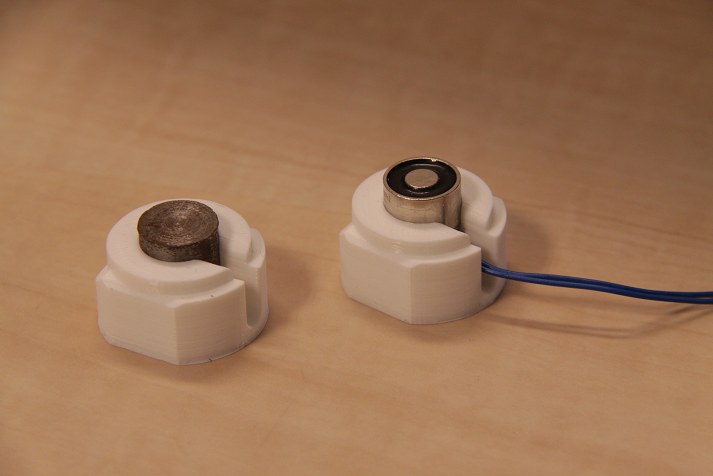
\includegraphics[width=0.95\textwidth]{img/IMG_4812_downsized}
			\caption{An active (right) and passive (left) magnetic connector in a (white) 3D-printed hull mount.}
			\label{fig:solenoidsMF}
		\end{minipage}\hfill
		\begin{minipage}{0.48\textwidth}
			\centering
			\includegraphics[width=0.95\textwidth]{IMG_4814_downsized}
			\caption{Active magnet mounted in the hull of a Delfia-1* module to connect modules into a rigid platform.}
			\label{fig:solenoids}
		\end{minipage}
	}
\end{figure}

\subsection{Network setup}
The backbone of the communication system is deployment of ROS over an internet network. Vessels connect over WiFi, while shore facilities connect to the network router through ethernet cables. ROS provides various standardized messagetypes to improve interoperability and modularity. Various conventions that are developed throughout this project are intended to serve as a framework for further development and reasearch in the facilities of Researchlab Autonomous Shipping. The proposed standardization includes:
\begin{itemize}
	\item ROS message types for control related signals
	\item Naming convention for control related ROS-topics
	\item IP adress reservations for vessels and other components
\end{itemize}
Table \ref{tab:ROSmsgTypeTable} shows the proposed conventions for communication over ROS in RAS facilities. 

\begin{table}[H]
	\centering
	\begin{tabular}{lll}
	Topic content & Messagetype & Naming convention \\[10pt] \hline
	Vessel position and orientation	&$geometry\_msgs/PoseStamped$ &  $/vrpn\_client\_node/<vesselname>/pose$    \\[10pt]
	
	Vessel Actuation	&   $std\_msgs/Float64MultiArray$     & $/actuation<vesselname>$  \\[10pt]
	
	\begin{tabular}[c]{@{}l@{}} Controller reference (for surface \\ plane dynamic positioning systems) \end{tabular} & $ geometry\_msgs/Pose2D$ &   $ /reference<controllername> $
	\end{tabular}
	\caption{Proposed conventions for communication over ROS in facilities of Researchlab Autonomous Shipping.}
	\label{tab:ROSmsgTypeTable}
\end{table}

The module state estimation system, consisting of a set of camera's and a device that interprets the image data, streams its poses of each module on the dedicated topics. The fleet control system uses this information to make decisions for a set of actuators, and broadcast it. Actuators throughout the fleet respond to such updates, closing the control loop. It is worth noting that the shown division of tasks leaves the system rather modular. Systems performing control and state estimation can be replaced, without the need of adapting other components given that these communication protocols are followed. The location and hardware on which a task is performed also becomes flexible. Furthermore, tasks can be divided, distributed, or centralized at the convenience of the designer, without the need of drastic system changes. Localization has been centralized, as an on-shore motion tracking system provides higher accuracy with respect to alternatives that perform localization on board (e.g. leidar, radar, GPS, IMU, camera image localization). Control decisions are centralized, as an on-shore computer that has access to computational power many times higher than can be feasibly realized on board of the model scale vessels. 

The trend in this minimalistic approach is to not perform tasks on a ship if it is not nessecary to do so. This does have some effects to be considered. Firstly, the system becomes reliant on network performance and availability. Advancements in telecommunication industry and technology led to options for increased connectivity between devices. To name only some examples; rural areas are commonly covered with a 4g internet network, and devices creating local (wireless) networks have become widespread and affordable. Secondly, simplicity of modules benefits scaling to a higher amount of vessels. Less components will be present that can cause malfunction or requirements for maintenance. 

To connect a module to the network, an on-boar Raspberry-pi provides the link between ROS, over wifi, and the arduino, over serial USB protocol. A standardized operating system image of Ubuntu-mate has been developed to be cloned on all Raspberry-pi's on the Delfia fleet. This has been done with the goal of needing to configure as little as possible to the Raspberry-pi's settings after cloning. Python scripts running on the device uses a single parameter (vessel number) to operate properly and subscribe to the correct ROS topics following naming convention as shown in table \ref{tab:ROSmsgTypeTable}. Rapidly setting up on-board Raspberry-pi's is valued so highly, as future changes that need to be applied on a large number of devices will become more laboursome. 

\subsection{Control Software}
\label{sec:controlSoftware}
Control decisions are made on a single device, where scripts are developed using Matlab as programming language. This software interacts with the network only through ROS, which means that it could have been developed in other languages as well thanks to the interoperability of ROS. This choice comes down to a matter of the developer's preference, and other options such as Python can be suitable as well.

In an effort to develop a matlab fleet-control-framework that is understandable, scalable and re-usable in future projects, an object-oriented structure is formed. Main functionality of the framework that forms the key elements of the feedback control loop are described further in this section. Sourcecode can be found in appendix \ref{appendix:algorythsms}. Classes that make up the framework  can be shortly described as follows:
\begin{itemize}
	\item A \textbf{Vessel} superclass provides basic traits and methods that are relvant for managing a single ship in 3 degrees of freedom on the surface plane. Various vessel types, such as the Delfia, Tito-Neri and Grey-Seabax types from the RAS-fleet, can inherit common characteristics and methods from this class. Some examples of key parameters are: state (positions and velocities), mass, vessel width and length. 
	\item The \textbf{Delfia} object class, subclass of Vessel, contains information and methods unique to the Delfia-1* robot. It is distinguished by various aspects such as: actuator setup with two azimuth thrusters, actuator-model, and methods that aid the standardized interaction through the ROS network. 
	\item The \textbf{Platform Controller} object class stores information and provides methods required on a platform level. This object's main function is running the feedback control loop for the platform consisting of multiple vessels. To do so, it contains and uses methods for platform-model estimation, control-system adaptation, platform-state estimation,  control effort generation, control effort allocation and communication over ROS. 
	\item The \textbf{Fleet Manager} object class acts as an overarching entity that dictates tasks of  controllers in a phasewise fashion. It provides control objectives for the platform controllers to use as a reference, and allocates ownership of a module to the platform controller to which a module is assembled. 
\end{itemize}

A control loop revolves primarily around a Platform Controller (referred to as 'controller' in this section), performing tasks of which the design is described in section \ref{sysdesign:Architecture}. Modules, represented as the Delfia class can be connected to- or disconnected from a platform trough the $attacgBody()$ and $detachBody()$ functions. This automatically triggers protocols that adjust functionality of the control loop to it's new configuration. Such functions are: 
\begin{itemize}
	\item Estimating the platform's centre of gravity
	\item Forming an estimate of the platform's dynamical model
	\item Adjusting gains of PID controllers that generate control effort
	\item Adjusting parameters affecting distribution of control effort between actuators.
\end{itemize}

The control loop runs event-driven, responding on position updates of the first connected module. As the optical motion tracking system publishes a module's pose, callbacks in the respected Delfia object update the position, and the platform initates it's control loop iteration which runs the following key steps
\begin{itemize}
	\item The platform starts by estimating it's current state from the updated module position and the known configuration of that module with respect to the platform. 
	\item The new state is fed alongside the reference to the parralel PID controllers. These three conrollers output desired control effort for all dimentions. This thus results in two desired forces along the platform's local x and y axis, and a desired resulting moment around z. 
	\item The desired control effort is then allocated between the actuators of all connected modules. Allocation occurs by individually allocating each force and moment, which is then combined into a solution that satisfies all control efforts simultaneously. 
	\item Finally, allocated control efforts (which are forces for each thruster in x and y direction) are translated to actuator commands (thruster angle and propeller speed). These commands are then published on ROS-topics dedicated to actuation for each respective module, such that they are executed by the physical vessel. 
\end{itemize}

\subsection{Modifications throughout development}
\label{AdjustmentsAfterTests}
The overall fleet control system underwent many iterative changes of which some key considerations are discussed here. First, the process of developing control gain tuning is discussed. Secondly, changing approaches for succesful assembly are discussed. Varying responses from systems with different settings have shown behaviors that are interesting to analyze. Off course not all responses show behavior that is particularly interesting, so only a selection is discussed.

%\subsubsection{Control Gain adaptation}
As mentioned in section \ref{sysdesign:Architecture}, control parameter tuning is done according to a particular reference configuration. The chosen reference configuration is a single module body. Step responses of movement in the three degrees of freedom (x,y,yaw) were evaluated to aid decision making for optimizing control behavior. The key measures of performance that are optimized throughout iterations are rise-time, settlingtime and overshoot. Amplitude of step inputs are based on a characteristic motion for a platform performing a logistical task. Translational movement is assumed to be a short distance, in the order of several times the length of the platform. This lead to the choice of amplitude in x and y reference of 1.0 and 0.5 meter. A characteristic rotation is set to a 90 degree turn. 

PID control gains are developed with the following approach \cite{PIDIntroMIT}
\begin{itemize}
	\item Add proportional control to improve the rise time
	\item Add a derivative control to reduce the overshoot
	\item Add an integral control to reduce the steady-state error
	\item Iteratively adjust each gain to improve the overall response 
\end{itemize}


Effects of control gains on system performance indicators can generally be described as in table \ref{tableKEffects}.
\begin{table}[H]
	\centering
	\captionsetup{justification=centering}
	\caption{Effects of independent P, I, and D tuning \citet{ang2005pid}}
	\label{tableKEffects}
	\begin{tabular}{llllll}
		\cline{1-6}
		%\rowcolor[HTML]{EFEFEF} 
		\textbf{Closed-Loop Response} & \textbf{Rise Time} & \textbf{Overshoot} & \textbf{Settling Time} & \textbf{Steady-State Error} & \textbf{Stability} \\ \cline{1-6}
		Increasing Kp                 & Decrease           & Increase           & Small Increase         & Decrease                    & Degrade            \\
		Increasing Ki                 & Small Decrease     & Increase           & Increase               & Large Decrease              & Degrade            \\
		Increasing Kd                 & Small Decrease     & Decrease           & Decrease               & Minor Change                & Improve            \\ \cline{1-6}
	\end{tabular}
\end{table}

Initial proportional gains were chosen based on characteristic initial error, maximum control effort and desired fraction of utilization of maximum control effort at the step time. Initial error is assumed equal to the step amplitude, and maximum control effort for single vessel operation could be calculated from the known thruster setup. Table \ref{orderDegreeSystemSingleDelfia} shows units and order of magnitude of forces, errors and rise times. 
\begin{table}[H]
	\centering
	\captionsetup{justification=centering}
	\caption{Maximum control effort of a single Delfia-1* vessel}
	\label{orderDegreeSystemSingleDelfia}
	\begin{tabular}{lll}
		System parameter                             & Order of magnitude & Unit      \\[2pt] \hline
		Max. control effort: translation - Force & fmax = 0.45        & {[}N{]}   \\
		Max. control effort: rotation - Torque   & mmax = 0.06        & {[}Nm{]}  \\
		Step amplitude: translation                  & 1.0          & {[}m{]}   \\
		Step amplitude: rotation                     & $\frac{1}{2} \pi$  & {[}rad{]} \\
		Rise time: translation (amp = 1.0 m)         &  6.0                  & {[}s{]}   \\
		Rise time: rotation  (amp = $\frac{1}{2} \pi$ rad)        &  2.0                  & {[}s{]}  \\ \hline
	\end{tabular}
\end{table}

Step responses for single vessel operation has been collected from three simultaneous, but independently operating modules. Figure \ref{stepXYYAW1example} illustrates how such step responses were executed. The step in reference occurs along the $x_{n}$ direction, after the system settled to it's initial reference. A 1.0 m translational step occurs in $x_n$ around $t\approx0s$. A pi/2 rad rotational step occurs at $t\approx110s$. A 0.5m translational step occurs in $x_n$ around $t\approx210s$. The translational steps are both in global x coordinate, yet they represent 'forward' and 'sideways' motion as the platform rotated in between. All modules respond fairly identical, as can be observed from the similarities of vessel response signals in x and $\Psi$ dimentions. It is worth noting how some coupling between degrees of freedom is visible, as a step in one dimention result in some, albeit small, distortions in the others. 

\begin{figure}[H]
	\centering
	\includegraphics[width=1.0\textwidth]{matlabEvaluationFig18a.eps}
	\caption{3 separate vessels doing the similar step responses, but at an y-offset, such that they are besides oneanother. Three different step responses are done in this test representing forward, rotational and sideways motion.}
	\label{stepXYYAW1example}
\end{figure}

Throughout the process of iteratively improving control performance by adjusting gains, various insights were gained. 
A steady state error for all step responses was neglectably small without utilizing any integral control. This can be explained by the fact that the test setup was in a lab setting with little to no disturbances such as wind, current or waves. Thus there was no nessecity of setting any integral gain.
Dampening that was naturally present on the vessels proved to be quite significant without addition of derivative control. This is obviously thanks to hydrodynamic dampening. Enough dampening was considered to be naturally present in translation, and addition of more dampening terms only decreased performance. However, rotational motion did benefit from derivative control, as way more oscillation could be noticed in the responses. Magnitude of derivative gain for rotational motion formed as a balance between rise-time and settling-time. 

Hence the control gain tuning process formed control gains from the reference configuration. Following the control-gain scaling approach as described in section \ref{controlEffortGenerationDesign}, the configuration-independent control gains were set as follows
\begin{table}[H]
	\centering
\begin{tabular}{llll}
Dimention & Proportional gain & Integrator gain & Derivative gain \\
	\hline & & & \\[-5pt]
	translation $x$ and $y$ 	& $1.0$ $[m^{-1}]$		& $0$ $[s*m^{-1}]$ &  $0$  $[s^{-1}m^{-1}]$\\[3pt] 
	rotation $\Psi$ 			& $0.4456$ $[rad^{-1}]$			& $0$ $[s*rad^{-1}]$ & $0.15$ $[s^{-1}rad^{-1}]$\\ 
	\hline 
\end{tabular}
\caption{Configuration independent control gains that resulted from iterative system response evaluation and tuning.}
\end{table}

%\subsubsection{Adjustments on the assembly protocol}
The initial assembly protocol has been slightly adjusted throughout initial experiments. Early tests on platform assembly proved unable to perform within a reasonable timeframe. This was caused due to the fact that the magnet connectors did not reliably come into the area of acceptance upon which they would connect. Magnets seemed an attractive solution to connecting, especially as there was not a required approach direction during connecting, but vessels simply had to be adequately close to oneanother. Practically, modules would indeed be positioned in assembly orientation, yet oscillate a little, and not properly coming into contact. The area of acceptance proved too small for timely assembly with the current approach. The difficulties during connecting are visible in one test in particular, for which the module references and responses are shown in figure \ref{tp8_connecting_overall}. During this test the assembly protocol ran as described in section \ref{assemblyProtocolDesign} and illustrated in figure \ref{fig:matlabEvaluationFig14c}.

\begin{figure}[H]
	\centering
	\includegraphics[width=1.0\textwidth]{tp8_connecting_overallb.eps}
	\caption{System responses during early connecting protocol. Notice how $x$ and $yaw$ reference remains constant. Most notably is the change in $y$ reference at $t=80s$. Assembly preparation and initial line-up occurs until this moment, after which the reference changes such that the vessels move to connection position.}
	\label{tp8_connecting_overall}
\end{figure}

From approximately $t=100$ one would expect modules to be approximately lined up such that magnet connectors could properly function. Successful connection can be judged in a more quantitative manner by expressing relative motion between modules. Succesful connections between modules should display zero or near zero relative motion. Figure \ref{tp8_connecting_relative_wide} \ref{AsseblyFailedRelative} show relative position between modules. For this, the body fixed frame of the middle vessel (module 2) is used, in which position of the connecting vessels (1 \& 3) are expressed (see figure \ref{fig:localframeShowing} for an illustration on how to interpret expressing location of a module in another vessel's body fixed coordinate system). 

\begin{figure}[H]
	\centering
	\includegraphics[width=0.9\textwidth]{tp8_connecting_relative_wide.eps}
	\caption{Relative motion of two modules connecting to module nr. 2, while running early assembly protocols.}
	\label{tp8_connecting_relative_wide}
\end{figure}

\begin{figure}[H]
	\centering
	\includegraphics[width=0.9\textwidth]{tp8_connecting_relative_Zoomed.eps}
	\caption{Relative motion of two modules connecting to module nr. 2, while running early assembly protocols. Relative motion of a module stops in all three degrees of freedom, more or less at the same time, indicating succesful connection.}
	\label{AsseblyFailedRelative}
\end{figure}

Although connection was succesfully achieved, it required a period in the order of 70 seconds, which was considered rather long, even for a proof of concept. It was observed that modules were positioned near the connection site, but with lacking stimulants to get connectors into area of acceptance. Figure \ref{tp8_connecting_relative_state130t} illustrates how modules float around the connection site, while they were unconstrained in three degrees of motion, resulting in discrepancy in x y and yaw positioning.  Small errors in the definition of the body-fixed frame of the modules obtained from the optical tracking system, can be seen in figure \ref{AsseblyFailedRelative} and \ref{tp8_connecting_relative_state130t}, as the former shows nonzero $x$ and $\Psi$ values after connecting and the latter shows a seeming overlap of vessels. Relative motion in three degrees of freedom are present, which causes the modules to be misaligned, making succesful connecting less probable. Seeming overlap of module 1 \& 2 is caused by small errors in the definition of modules' origins. The definitions of the module's origins with respect to the optical trackers were slightly adjusted to decrease the magnitude of these errors for further tests. 

\begin{figure}[H]
	\centering
	\includegraphics[width=0.7\textwidth]{tp8_connecting_relative_state130t.eps}
	\caption{Measured system state at $t=130s$ during early assembly test shown in figure \ref{tp8_connecting_relative_wide} and \ref{AsseblyFailedRelative}.}
	\label{tp8_connecting_relative_state130t}
\end{figure}
The problem of being insufficiently able to position modules within connector area of acceptance was solved by using normal forces on the modules' hulls to align surfaces. This is a common trick used by regular, human operated ships. A characteristic example is a ferry that pushes itself to a dock, such that it does not rotate or move, allowing safe transfer of passengers. A small normal force between vessels ensures that they keep making contact, and avoid rotation. As modules made contact, only one motion remained, which was translation along the contact surface. With only one degree of (relative) motion connections could be made timely. Figure \ref{DelfiasNormalForceIntoPush2} shows how normal forces have been created by setting contoller reference somewhat within the rigid body of a neighbouring module. Figure \ref{tp8_connecting_relative_wide} shows relative motion between modules of an assembling system that apply this approach. Notice that relative rotation and motion perpendicular to the contact surface are constrained first. Sliding motion along contact surface later stops as connectors snap into place. 

 \begin{figure}[H]
	\centering
	\makebox[\textwidth][c]{
		\begin{minipage}{0.47\textwidth}
			\centering
			\includegraphics[width=1\textwidth]{img/3x1ConfigurationRef}
			\caption{Initial reference positions of modules for assembly}
			\label{3x1ConfigurationRef}
		\end{minipage}\hfill
		\begin{minipage}{0.45\textwidth}
			\centering
			\includegraphics[width=1\textwidth]{img/3x1ConfigurationRef_overlapping}
			\caption{Adjusted references for positioning of modules while connecting, to create some normal forces between hulls. The shown references are impossible for the system to reach, as vessels are constrained by their hulls which can not overlap.}
			\label{3x1ConfigurationRef_overlapping}
		\end{minipage}
	}
\end{figure}

\begin{figure}[H]
	\centering
	\includegraphics[width=0.4\textwidth]{VesselConnectTopvieuwReference_early.eps}
	\caption{Normal forces that result from overlapping references during assembly.}
	\label{DelfiasNormalForceIntoPush2}
\end{figure}

The normal forces between modules were kept to a minimum, as they purely function to remove motion between vessels perpendicular to the connection surface ($y$), and rotation. Remaining motion was by sliding along the connecting surface of the hull ($x$ direction), where friction did not seem to play a significant role with a smooth surface and low normal forces. 



\vspace{15mm}

This chapter explained design choices that characterize the developed self-assembling and cooperative fleet control system. At first, the multi-robot control approach with variable topology is explained after which the design of each subsystem is discussed. Implementation is thereafter explained, showing the realization of the fleet control system. The next chapter will assess performance of the  developed framework, to see whether or not the system performs according to the presented design criteria and goals. 


	\chapter{Evaluation}
\label{chap:evaluation}

This chapter evaluates the performance of the developed fleet control system. Evaluation is done in two steps, namely in terms of assembly and motion control behavior. 

Evaluation starts with a focus on the task of automated assembly. After that, motion control performance is evaluated for two platform configurations; a single vessel scenario and a 3x1 assembled platform. Results of system behavior are presented and performance is quantified. System evaluation concludes by comparing system behavior with the design criteria discussed in section \ref{sysdesign:Architecture} 

\section{Assembly}
\label{evaluateAssembly}
This section discusses the performance of the system's ability of automated self assembly. Evaluation starts in a more general sense and ends in a quantitative manner. A variety of system responses performing assembly have been collected throughout this project from system iterations. The results that are discussed in this section are from the most final version of the platform assembly proceidure, of which the overall design is discussed in section \ref{assemblyProtocolDesign}, with minor implementational changes as discussed in section \ref{AdjustmentsAfterTests}. 

Performance of reconfiguration will be quantified by evaluating the change in relative pose between neighbouring modules in all considered degrees of freedom. Pose of vessel $j$ with respect to vessel $i$ expressed in the body fixed coordinate system of vessel $i$ is expressed as:

\begin{equation}
\eta_j^i = \begin{bmatrix} \textbf{p}^{i}_{j} \\[8pt]  \Theta_{ij} \end{bmatrix} = \begin{bmatrix} x^{i}_{j} \\[8pt]  y^{i}_{j} \\[8pt] \Psi^i_j \end{bmatrix}
\label{PerfIndicatorRelativePose}
\end{equation}


The overall system response during assembly is shown in figure \ref{AssemblyGoodGlobal_tp14}, which shows poses of the modules in the degrees of freedom of the water surface. Figure \ref{AssemblyGoodGlobal_tp14} shows that the reference heading ($\Psi$) and $x$ position remains constant during the assembly protocol. Response in $y$ direction shows pre-assembly line up at $t<295$, after which the modules approach and finally connect.  

\begin{figure}[H]
	\centering
	\captionsetup{justification=centering}
	\includegraphics[width=0.9\textwidth]{VesselConnectAdjustedTotalMovementb}
	\caption{Module position plotted versus time, during the platform assembly stage. Vessels are initially lining up side-by-side, until they approach due to changin $y$ reference values. }
	\label{AssemblyGoodGlobal_tp14}
\end{figure}

Assembly succes or failure was easily detectable by eye, but can be supported quantitatively by evaluating relative motion. The two modules attempted assembly simultaneously which is shown in figure \ref{AssemblyGoodrelative_tp14}. Simultaneous plotting of relative pose of both module 1 \& 3 requires a rather large scale in $y$ direction which doesn't show a lot of detail. Therefor the relative pose of module 1 \& 3 are also individually plotted in figure \ref{connectFinal3DOF_delfia1} and \ref{connectFinal3DOF_delfia2} respectively.

\begin{figure}[H]
	\centering
	\captionsetup{justification=centering}
	\includegraphics[width=0.9\textwidth,center]{evaluationConnect_tp14_relativemotion_wideb}%
	\caption{Relative motion of assembling vessel system}
	\label{AssemblyGoodrelative_tp14}
\end{figure} 

 \begin{figure}[H]
 	\centering
 	\captionsetup{justification=centering}
 	\includegraphics[width=0.9\textwidth,center]{connectFinal3DOF_delfia1}%
 	\caption{Relative motion of module 1 expressed in body fixed frame of module 2. }
 	\label{connectFinal3DOF_delfia1}
 \end{figure}

 \begin{figure}[H]
 	\centering
 	\captionsetup{justification=centering}
	\includegraphics[width=0.9\textwidth,center]{connectFinal3DOF_delfia2}%
	\caption{Relative motion of module 3 expressed in body fixed frame of module 2.}
	\label{connectFinal3DOF_delfia2}
\end{figure}

Some notes on the module's relative positions during assembly are considered worth discussing, particularly on the interpretation of the responses. 
The signals showing relative positions in figure \ref{connectFinal3DOF_delfia1} and \ref{connectFinal3DOF_delfia2} show some forms of plateauing behavior, which is particularly interesting. The slope of these signals becoming a plateau means that relative speed has suddenly become near zero. This is considered to be due to physical contact between hulls. This can be a bump, soft contact, or a connector snapping two modules together. 
Relative pose of both connecting modules show some similarities. Pose in various DOFs show plateaus where the speed suddenly becomes near zero, which are most clear in $y$ direction for both modules. Furhermore, a clear moment can be observed on which relative motion becomes near zero for not one, but all degrees of motion, indicating a succesful connection. 

Figure \ref{fig:EvaluationConnectTwoInstances_AllDofs} to \ref{stateDuringAssembly364} illustrate how the relative motion was interpreted for module 1 at two different timestamps. At $t = 308s$ rapid descelleration, is visible in figure \ref{fig:EvaluationConnectTwoInstances_AllDofs} in $y$ direction due to hull contact, while figure \ref{stateDuringAssembly308} shows that vessel 1 is still misaligned. Some motion and aligning occurs until relative motion suddenly halts, around $t = 364s$. This shows the connector performing to restrain relative motion in configured state, shown in figure \ref{stateDuringAssembly364}.

\begin{figure}[H]
	\centering
	\includegraphics[width=0.9\textwidth]{EvaluationConnectTwoInstances_AllDofs2}
	\caption{EvaluationConnectTwoInstancesAllDofs}
	\label{fig:EvaluationConnectTwoInstances_AllDofs}
\end{figure}

\begin{figure}[H]
	\centering
	\makebox[\textwidth][c]{
		\begin{minipage}{0.47\textwidth}
			\centering
			\includegraphics[width=1\textwidth]{img/stateDuringAssembly308}
			\caption{Fleet pose shown in a top-down-view at $t=308s$ while modules are aligning during assembly.}
			\label{stateDuringAssembly308}
		\end{minipage}\hfill
		\begin{minipage}{0.45\textwidth}
			\centering
			\includegraphics[width=1\textwidth]{img/stateDuringAssembly364}
			\caption{Fleet pose shown in a top-down-view at $t=364s$, as motion between modules became near zero.}
			\label{stateDuringAssembly364}
		\end{minipage}
	}
\end{figure}

To further quantify the remaining perceived motion after assembly of module 1, the dataset is evaluated from the moment of connecting (approximately at $t=364$) and 10 seconds thereafter. 

\begin{table}[H]
	\begin{tabular}{lllllll}
& & Average & Minimum & Maximum & maxAmpl & Variance \\ 
\hline 
$x$ &[m]& -0.0076628 & -0.0082233 & -0.0071825 & 0.0010408 & 4.3663e-08 \\ 
$y$ &[m]&-0.17236 & -0.17288 & -0.17198 & 0.00089951 & 2.6465e-08 \\ 
$\Psi$&[rad]& -0.018446 & -0.02136 & -0.014622 & 0.006738 & 1.0167e-06 \\ 
\hline 
\end{tabular}
	\caption{Signal analysis of relative motion of module 1 with respect to body-fixed frame of module 2 for $364<t<374$.}
	\label{tab:ConnectVariationTableOut}
\end{table}


\section{Platform Motion Control}
\label{evaluationMotionControl}
To evaluate the motion control performance of the developed framework, vessel system will be tasked to follow a time varying reference signal with step changes. Performance quantification is done by expressing rise-time and settling-time and overshoot (see fig \ref{fig:matlabStepresponseFig})of step responses to reference position of the platform in all considered degrees of freedom. Thoughout experiments steps in the platform's reference pose are given in one degree of freedom at a time. 

\begin{figure}[H]
	\centering
	\includegraphics[width=0.7\textwidth]{stepplot1}
	\caption{Interpretation of typical quantities illustrated that are used to characterize a second order system \cite{stepinfoWebMatlab}.}
	\label{fig:matlabStepresponseFig}
\end{figure}

Platform motion is evaluated for two scenario's; single vessel operation and 3x1 lattice platform configuration, as shown in figure \ref{1x1Config} and \ref{3x1Configuration}. Note that control parameter tuning occured in single vessel operation. Any other arbitrary configuration, including the tested 3x1 platform, is required to behave satisfactory due to the configuration-adaptability of the control system. 

 \begin{figure}[H]
	\centering
	\makebox[\textwidth][c]{
		\begin{minipage}{0.47\textwidth}
			\centering
			\includegraphics[width=1\textwidth]{img/1x1Config}
			\caption{A single Delfia configuration}
			\label{1x1Config}
		\end{minipage}\hfill
		\begin{minipage}{0.45\textwidth}
			\centering
			\includegraphics[width=1\textwidth]{img/3x1ConfigurationRef}
			\caption{A 3x1 platform configuration, which represented assembled platform state troughout experiments.}
			\label{3x1Configuration}
		\end{minipage}
	}
\end{figure}

Both scenarios get similar tasks of short displacements as a step input on the reference pose. These step responses are then evaluated to quantify this performance in post processing. Figure \ref{fig:tp21_steps} shows three step responses for single vessel controlled by the system. Figure \ref{fig:tp22_Steps3x} shows responses of a 3x1 configured platform. Responses of both configurations that are plotted have quantitative analysis parameters shown in tables \ref{tablev1x1} to \ref{tablev1yaw2}.

\begin{figure}[H]
	\centering
	\includegraphics[width=0.8\textwidth]{tp21_stepsb.eps}
	\caption{Step responses of single Delfia configuration. Responses are gathered by changing reference of a single degree of motion (x y and yaw) at a time. Three datasets are shown, which show that the responses are rather constant.}
	\label{fig:tp21_steps}
\end{figure}

\begin{figure}[H]
	\centering
	\includegraphics[width=0.8\textwidth]{tp22_Steps3xb}
	\caption{Step responses of a 3x1 lattice configuration. Responses are gathered by changing reference of a single degree of motion (x y and yaw) at a time. Two step responses are shown for each degree of motion.}
	\label{fig:tp22_Steps3x}
\end{figure}


Step responses are evaluated quantitatively in terms of rise-time, overshoot and settling-time, calculated by Matlab's 'stepinfo' function \cite{stepinfoWebMatlab}.  Rise time is defined as the time between a 10\% and 90\% rise of the signal. 
which are shown for all degrees of motion of both single and assembled configuration in tables \ref{tablev1x1} to \ref{tablev1yaw2}. The configured settling-time criteria is met if the signal is dampened within a factor of $0.05$ of the steady state value. 

\begin{table}[H]
	\captionsetup{justification=centering}
	\begin{adjustbox}{max width=1.3\textwidth,center}
		\begin{minipage}{.55\textwidth}
			\centering
			\begin{tabular}{llll}
  & RiseTime & SettlingTime & Overshoot  \\ 
  & $\;\;\;\;[s]$ & $\;\;\;\;[s]$ & $\;\;\;\;[\%]$  \\ 
\hline 
response1 & 2.803 & 27.7096 & 33.1361 \\ 
response2 & 2.3159 & 27.0722 & 38.8513  \\ 
response3 & 2.6438 & 26.6143 & 36.229  \\ 
Average & 2.5876 & 27.132 & 36.0721  \\ 
\hline 
\end{tabular}
			\caption{Single vessel $x$-direction step response evaluation}
			\label{tablev1x1}
		\end{minipage}%
		\begin{minipage}{.55\textwidth}
			\centering
			\begin{tabular}{llll}
  & RiseTime & SettlingTime & Overshoot  \\ 
  & $\;\;\;\;[s]$ & $\;\;\;\;[s]$ & $\;\;\;\;[\%]$  \\ 
\hline 
response1 & 2.9263 & 31.2773 & 38.7962  \\ 
response2 & 2.9202 & 45.2133 & 36.0778 \\ 
Average & 2.9232 & 38.2453 & 37.437  \\ 
\hline 
\end{tabular}
			\caption{Assembled 3x1 platform $x$-direction step response evaluation}
			\label{tablev1x2}
		\end{minipage}
	\end{adjustbox}
\end{table}

\begin{table}[H]
	\captionsetup{justification=centering}
	\begin{adjustbox}{max width=1.3\textwidth,center}
		\begin{minipage}{.55\textwidth}
			\centering
			\begin{tabular}{llll}
  & RiseTime & SettlingTime & Overshoot \\ 
  & $\;\;\;\;[s]$ & $\;\;\;\;[s]$ & $\;\;\;\;[\%]$  \\ 
\hline 
response1 & 4.4688 & 32.2703 & 30.6531  \\ 
response2 & 4.0913 & 31.7191 & 34.0618\\ 
response3 & 4.3417 & 35.8629 & 32.147  \\ 
Average & 4.3006 & 33.2841 & 32.2873 \\ 
\hline 
\end{tabular}
			\caption{Single vessel $y$-direction step response evaluation}
			\label{tablev1y1}
		\end{minipage}%
		\begin{minipage}{.55\textwidth}
			\centering
			\begin{tabular}{llll}
  & RiseTime & SettlingTime & Overshoot  \\ 
  & $\;\;\;\;[s]$ & $\;\;\;\;[s]$ & $\;\;\;\;[\%]$  \\ 
\hline 
response1 & 4.5348 & 32.9588 & 31.2256  \\ 
response2 & 3.3676 & 32.6829 & 33.3475 \\ 
Average & 3.9512 & 32.8209 & 32.2865  \\ 
\hline 
\end{tabular}
			\caption{Assembled 3x1 platform $y$-direction step response evaluation}
			\label{tablev1y2}
		\end{minipage}
	\end{adjustbox}
\end{table}

\begin{table}[H]
	\captionsetup{justification=centering}
	\begin{adjustbox}{max width=1.3\textwidth,center}
		\begin{minipage}{.55\textwidth}
			\centering
			\begin{tabular}{llll}
  & RiseTime & SettlingTime & Overshoot  \\ 
  & $\;\;\;\;[s]$ & $\;\;\;\;[s]$ & $\;\;\;\;[\%]$  \\ 
\hline 
response1 & 1.0576 & 6.1474 & 35.8941  \\ 
response2 & 0.97707 & 6.105 & 35.6279\\ 
response3 & 0.99748 & 6.0969 & 35.9651  \\ 
Average & 1.0107 & 6.1164 & 35.829 \\ 
\hline 
\end{tabular}
			\caption{Single vessel $\Psi$-direction step response evaluation}
			\label{tablev1yaw1}
		\end{minipage}%
		\begin{minipage}{.55\textwidth}
			\centering
			\begin{tabular}{llll}
  & RiseTime & SettlingTime & Overshoot  \\ 
  & $\;\;\;\;[s]$ & $\;\;\;\;[s]$ & $\;\;\;\;[\%]$  \\ 
\hline 
response1 & 1.2894 & 18.2124 & 40.2248  \\ 
response2 & 1.3382 & 12.8114 & 35.3374 \\ 
Average & 1.3138 & 15.5119 & 37.7811  \\ 
\hline 
\end{tabular}



			\caption{Assembled 3x1 platform $\Psi$-direction step response evaluation}
			\label{tablev1yaw2}
		\end{minipage}
	\end{adjustbox}
\end{table}


Tables \ref{tablev1x1} to \ref{tablev1yaw2} show quantitative indicators of performance of the system in two configurations. The graphs and tables show that the designed system is able to control various configurations. Step-response performance could be optimized more, but that is not the point. More important is learning from the scalability of this motion control system, as its novelty comes from using information about the platform's shape, size, and configuration. Thus, responses of single and assembled configuration will be compared. 

Recall from section \ref{controlEffortGenerationDesign} that configuration dependent platform motion control was designed with using an approximate time scale. This timescale took into account varying inertia and available control effort, with respect to the reference configuration (where reference configuration was implemented as a single vessel). 

Taking a look at the appoximate timescale for linear motion, it was found that the available thrust and inertia equally scaled linear to the amount of modules, since a homogeneous fleet is used. Thus maximum platform thrust scales as
\begin{equation}
	F_{platform,max} \approx n_{modules} * F_{single,max} 
\end{equation}
where $F_{platform,max}$ is maximum platform thrust when it fully utilizes all azimuth thrusters, $F_{single,max}$ is the maximum thrust of a single Delfia-1* module. Similarly, platform mass scales as
\begin{equation}
	m_{platform} \approx n_{modules} * m_{single} 
\end{equation}

Computing approximate time scale of linear platform motion using equation \ref{eq:timescaleDef} yields

\begin{equation}
C_{x,y} = \frac{F_{c} \; I_{ref}}{F_{ref} \; I_{c}} = 1
\label{eq:timescaleDef2}
\end{equation}
which is quite intuitive, as the maximum thrust to mass ratio remained constant.  Angular control effort and angular-inertia were appoximated to not scale similar. Values of estimated inertias and control effort are shown in table \ref{tab:inertiaAndControlEffortCompared}, which yield an approximate time constant for rotation of 

\begin{equation}
C_{\Psi}  = 1.2980
\label{eq:timescaleDefYaw}
\end{equation}
 


\begin{table}[h]
	\centering
	\captionsetup{justification=centering}
	\begin{tabular}{lll}
		& Inertia            & Maximum input  \\[10pt]  \hline
		\begin{tabular}[c]{@{}l@{}}Single vessel: \\ Translation\end{tabular}  & $4.1275kg$& $0.4320N$ \\[10pt] %\hline
		\begin{tabular}[c]{@{}l@{}}Single vessel:\\ Rotation\end{tabular} & $0.1410 kg* m^2$ & $0.0670N*m$  \\[10pt] %\hline
		\begin{tabular}[c]{@{}l@{}}3x1 Configuration:\\ Translation\end{tabular} & $12.3825 kg$  & $1.2960 N$  \\[10pt] %\hline
		\begin{tabular}[c]{@{}l@{}}3x1 Configuration:\\ Rotation\end{tabular}  & $0.7091 kg*m^2$ & $ 0.2596 N*m$   \\ \hline
	\end{tabular}
	\caption{Approximate scaling of reference and assembled configuration}
	\label{tab:inertiaAndControlEffortCompared}
\end{table}

Correctness of using the assumption of the used timescale can be evaluated by comparing response times of reference and assembled configuration. This will show to what extent the system maintains similar behavior over changing configurations, which will give indicators how it might behave for other configurations. 



\begin{table}[H]
	\centering
	\captionsetup{justification=centering}
	\begin{tabular}{lllll}
 & RiseTime & SettlingTime & Overshoot & PeakTime \\ 
 & $\;\;\;\;[s]$ & $\;\;\;\;[s]$ & $\;\;\;\;[\%]$ & $\;\;\;\;[s]$ \\ 
\hline 
Single module & 2.5876 & 27.132 & 36.0721 & 7.2288 \\
3x1 conf. & 2.9232 & 38.2453 & 37.437 & 7.6737 \\[10pt] \hline 
Ratio & 1.1297 & 1.4096 & 1.0378 & 1.0615 \\ 
\end{tabular}
	\caption{Comparison between step responses of reference (single vessel) and adapted (3x1) configuration of linear motion in x direction}
	\label{table_evaluationDifference_dimentionx}
\end{table}


\begin{table}[H]
	\centering
	\captionsetup{justification=centering}
	\begin{tabular}{lllll}
  & RiseTime & SettlingTime & Overshoot & PeakTime \\ 
 & $\;\;\;\;[s]$ & $\;\;\;\;[s]$ & $\;\;\;\;[\%]$ & $\;\;\;\;[s]$ \\ 
\hline 
Single vessel configuration & 4.3006 & 33.2841 & 32.2873 & 11.0471 \\ 
3x1 configuration & 3.9512 & 32.8209 & 32.2865 & 10.4886 \\[10pt] \hline
Ratio & 0.91876 & 0.98608 & 0.99998 & 0.94944 \\ 
\end{tabular}
	\caption{Comparison between step responses of reference (single vessel) and adapted (3x1) configuration of linear motion in y direction}
	\label{table_evaluationDifference_dimentiony}
\end{table}


\begin{table}[H]
	\centering
	\captionsetup{justification=centering}
	\begin{tabular}{lllll}
 Dimention: yaw & RiseTime & SettlingTime & Overshoot & PeakTime \\ 
 & $\;\;\;\;[s]$ & $\;\;\;\;[s]$ & $\;\;\;\;[\%]$ & $\;\;\;\;[s]$ \\ 
\hline 
Single vessel configuration & 1.0107 & 6.1164 & 35.829 & 2.3432 \\ 
3x1 configuration & 1.3138 & 15.5119 & 37.7811 & 2.8033 \\[10pt] \hline
Ratio & 1.2999 & 2.5361 & 1.0545 & 1.1964 \\ 
\end{tabular}
	\caption{Comparison between step responses of reference (single vessel) and adapted (3x1) configuration of rotational motion in yaw direction}
	\label{table_evaluationDifference_dimentionyaw}
\end{table}

To evaluate control system adaptation performance the ratio between performance indicators of reference and configured state is used from table \ref{table_evaluationDifference_dimentionx} to \ref{table_evaluationDifference_dimentionyaw}. 

\textbf{Overshoot} seems to remain rather constant, varying $3.78\%$,$0.002\%$ and $5.45\%$ for $ x$,$y$ and $\Psi$ motion respectively. 

The \textbf{rise-time} of linear motion somewhat behaves according to the approximate timeconstant of $1$ (equation \ref{eq:timescaleDef2}). The risetime ratios of $1.1297$ and $0.91876$ for x and y motion are quite near the approximated scaling of $1.0$. Differences can be explained by the fact that the implemented control system does not use directional dependent mass or dampening for linear motion. Platform mass was approximated as constant in all directions for adapting PID gains, as the position controllers used global coordinates. 

The rise-time of angular motion changed with a ratio of $1.299$, which is rather close to the approximated time constant of $C_{\Psi}  = 1.2980$ (\ref{eq:timescaleDefYaw}).

\textbf{Settling-time} varied significantly between some measurements, such as the in the x-response of the assembled configuration (table \ref{tablev1x2} settlingtimes of $31.2773$ and $45.2133$ s ). This is peculiar as the two responses in x direction plotted in figure \ref{fig:tp22_Steps3x} are very much alike. The steady state criteria was reached half a period later, but with the long periods of oscillation (in the range of ~20 seconds), this resulted in a significant difference in settling time. Applications that highly value the performance indicator of settling time are recommended to rethink appropriate settling criteria. 
Most other settling times seemed rather consistent throughout datasets, with the exception of rotation of the assembled platform. Two rotation responses of the assembled platform (figure \ref{fig:tp22_Steps3x}, $\Psi$ dimention ) show identical behavior on the first period, yet seem to show some difference in oscillation dampening, which are in line with the different settling times ( table \ref{tablev1yaw2}).

Collaborative distribution of control effort was aimed to perform in a coordinated fashion. Figure \ref{forceArrows_3x1_tp22_t84} to \ref{fig:3x3_forcePlatformMotionIllustrative} show various independent and combined modes of motion in 3x1 assembled configuration, illustrating how the control allocation protocol assigns tasks to actuators.

%\colorbox{yellow}{\parbox{12cm}{ Is this the best place to illustrate the control allocation protocol in action?}}\\

 \begin{figure}[H]
	\centering
	\makebox[\textwidth][c]{
		\begin{minipage}{0.47\textwidth}
			\centering
			\includegraphics[width=1\textwidth]{img/forceArrows_3x1_tp22_t84}
			\caption{Control effort allocated to create (almost) pure force in x direction.}
			\label{forceArrows_3x1_tp22_t84}
		\end{minipage}\hfill
		\begin{minipage}{0.45\textwidth}
			\centering
			\includegraphics[width=1\textwidth]{img/forceArrows_3x1_tp22_t184}
			\caption{Control effort allocated to create pure torque about CM.}
			\label{forceArrows_3x1_tp22_t184}
		\end{minipage}
	}
\end{figure}

 \begin{figure}[H]
	\centering
	\makebox[\textwidth][c]{
		\begin{minipage}{0.47\textwidth}
			\centering
			\includegraphics[width=1\textwidth]{img/forceArrows_3x1_tp22_t287}
			\caption{Control effort allocated to create (almost) pure force in body-fixed-y direction.}
			\label{X}
		\end{minipage}\hfill
	
	}
\end{figure}

\begin{figure}[H]
	\centering
	\makebox[\textwidth][c]{
		\centering
		\includegraphics[width=1.3\textwidth]{3x3_forcePlatformMotionIllustrative}
	}
	\caption{Various timeframes of motiontest-22 moving to a reference position ($\times$) involving simultaneous rotation and translation. Arrows depict thruster forces, showing combined control effort (forces in various directions and torque) allocated and distributed over the platform's modules.}
	\label{fig:3x3_forcePlatformMotionIllustrative}
\end{figure}

\section{Comparing results with design criteria}

Section \ref{sysdesign:Architecture} starts describing design criteria which are evaluated here. 

Firstly, the system is required to perform automated vessel platform reconfiguration. This criteria is reached as has been observed throughout operation (by seeing magnet connectors snap into place), yet this is quantitatively supported by expressing relative module motion in section \ref{evaluateAssembly}. Figure \ref{fig:EvaluationConnectTwoInstances_AllDofs} illustrates a typical sudden stop in relative vessel motion in all degrees of freedom indicating succesful connection. Assembly of the final developed system behaved consistently throughout testing. Tab. \ref{tab:KPIresultsAssembly} shows how relative motion after connection was quantified, being near zero, compliant with the set design criteria. 

% Please add the following required packages to your document preamble:
% \usepackage{multirow}
\begin{table}[H]
	\centering
	\begin{tabular}{llllc}
		Motion & \multicolumn{1}{c}{\begin{tabular}[c]{@{}c@{}}Maximum\\ signal amplitude\end{tabular}} & Variance   & Criteria                  & \multicolumn{1}{l}{Compliant} \\ \hline
		x      & 0.0010408 m                                                                            & 4.3663e-08 & \multirow{3}{*}{$\approx 0$} & \checkmark                             \\
		y      & 0.00089951 m                                                                           & 2.6465e-08 &                           & \checkmark                             \\
		$\Psi$    & 0.006738 rad                                                                           & 1.0167e-06 &                           & \checkmark                            
	\end{tabular}
	\caption{Key performance indicators regarding assembly and compliancy versus design criteria.}
	\label{tab:KPIresultsAssembly}
\end{table}


Secondly, the system needs to perform motion control in a collaborative manner, where multiple robots work together to achieve a single goal. Centralizing platform control to a single entity facilitated modules contributing to reaching one objective and allowed coordination strategies to increase actuator usage effectiveness. Figure \ref{fig:tp22_Steps3x} displays responses to reference step changes of a 3x1 lattice configurated platform, showing how the developed system controls to converging and stabilizing at reference state. 

% Please add the following required packages to your document preamble:
% \usepackage{multirow}
\begin{table}[H]
	\centering
	\begin{tabular}{lllllll}
		\multirow{2}{*}{Configuration vs KPI} & \multicolumn{2}{c}{Risetime}                                         & \multicolumn{2}{c}{Settlingtime}                                     & \multicolumn{2}{c}{Overshoot}                                       \\
		& \multicolumn{1}{c}{Criteria}        & \multicolumn{1}{c}{Compliancy} & \multicolumn{1}{c}{Criteria}        & \multicolumn{1}{c}{Compliancy} & \multicolumn{1}{c}{Criteria}       & \multicolumn{1}{c}{Compliancy} \\ \cline{1-7} 
		Single module configuration           & \multirow{2}{*}{t\_r \textless 10s} & 100\%                          & \multirow{2}{*}{t\_s\textless{}40s} & 100\%                          & \multirow{2}{*}{os\textless{}50\%} & 100\%                          \\
		3x1 platform configuration            &                                     & 100\%                          &                                     & 83,3\%                         &                                    & 100\%                         
	\end{tabular}
	\caption{Key performance indicators regarding motion control of all degrees of motion.}
	\label{tab:KPIresultsMotion}
\end{table}


The last hard design criteria requires the developed system to perform the two abovementioned behavioral criteria simultaneously. Reconfiguration and configuration dependent platform motion control operated within the same framework, where control approach changed in troughout operation as a response to platform assembly. 

%The following evaluation is done according to criteria which were considered not crucial, yet still desirable.

The designed framework theoretically supports motion control of any arbitrary configuration, as whas desired. Experiments were conducted on two quite general shapes that both showing satisfactory responses. The control approach adapts to unknown configurations by using scaling rules aimed to be representative over a wide variety of shapes and sizes. Although scaling rules have been designed relying on physics, used assumptions need to be re-evaluated for correctness of future configurations, particularly with more extreme shapes and scales. 

The framework was developed aimed to represent a logistic solution that could be implemented in the near future. Off course full scale commercial adoption will bring some challenges that were not present in the experimental lab setup, such as disturbances due to wind and current.  All system components are considered replacable for other solutions that might better fit more realistic scales, requirements and environments. 

Replacing or improving components of the system is stimulated by making the control framework as modular as possible. Various subsystems can be further developed, which was expected as exploration of a novel combination of behaviors was the goal rather than optimization.

From this evaluation it is concluded that the system developed througout this project is compliant with the set design criteria. 


\vspace{15mm}

This evaluation and findings throughout the process of system development are presented in the next chapter to conclude this project, mention points of discussion and present the author's view on future research directions. 

	\chapter{Conclusion}
\label{Conclusion}
This paper presents systematic development steps and design choices to realize a multivessel system able to configure vessels into interconnected platforms while performing perform configuration dependent collaborative control. 

The developed framework was designed to reflect a scenario of an automated fleet system with the task to solve a logistical problem, by forming floating infrastructure in a predefined shape that can be loaded, which subsequantially needed to perform motion tasks. Implementation serves as proof of concept, which is evaluated as performing compliant to the set design criteria. Full scale commercial adoption will bring more challenges that were not present in the experimental lab setup, such as disturbances due to wind and current.  Used design approach is considered applicable to other scales and environments as all system components are considered replacable for other solutions better serving requirements of the usecase.

The research approach relied on searching answers to the following main research question ans subquestions:

\noindent {\large\textbf{ Main research question}}
\begin{itemize}
	\item How can a fleet of modular surface platform vessels be controlled to achieve automated assembly and configuration-dependent platform control?
\end{itemize}
\noindent {\large\textbf{Sub-questions}}
\begin{enumerate}
	\item What is the state of the art within automated vessel platforming systems?
	\item What characteristics does a vessel system have that integrates automated assembly with configuration dependent control?
	\item How can the dynamics of the multi-vessel system be represented?
	\item How can a fleet control framework be developed that performs automated platform assembly and configuration adaptive platform control? 
	\item What is the performance of the developed system?
\end{enumerate}

Literature survey describes major literature of projects related to vessel self-assembly and collaborative control approaches to answer the first subquestion. The review describes various works categorized as 'vessel platform self-assembly' and one project showing development of a 'collaborative and coordinated multi-vessel-platform control'. It seemed natural that modular vessel platform automation will encompass behavior of both categories in the near future to become of highest societal benefit. Yet no sources were found describing both behaviors integrated in a single system, leading to the gap of knowledge that this project adresses. 

A more in depth look is given to the definition of multi-robot systems that perform 'self-assembly' and 'collaborative, coordinated control' to answer the second subquestion. This section significantly relied on literature works to map characteristics of both systems from different perspectives. Works with a general robotics perspective (versus marine robotics) were shown to have significantly more extensive descriptions of traits, design choices and categorizations, and thus were included within characterization efforts.  It was shown that many approaches were possible to design the discussed systems, each with their own benefits and limitations with different probable usefulness for logistic purposes. Generalized system characteristics are distinct and narrowed down set of solutions that can be considered more feasible to perform in commercial applications, taking into account the design trend in other projects and their emergent characteristics.

A multi-vessel state description is proposed, together with a novel approach to predict dynamics of a combined waterborne structures to answer the third subquestion. Existing (single) vessel state descriptions are extended to formulate this multi-vessel state description aiming to enable consistent system notation of scenarios pertaining more than a single object (vessels, coordinate systems) that can be referred to. Furthermore, the concept and definition of a platform-coordinate system is introduced. This resulted in three distinct types of coordinate systems; vessels, assemblies/platforms and global (e.g. inertial) frames that define state of an object and coordinate system in which parameters of other objects (pose, velocities, forces) can be expressed. 
The proposed approach to predict dynamics of a combined waterborne structure utilizes superpositioning of module models into a combined platform model as alternative of parameter estimation experiments for variable configurations. Particular emphasis is given to taking into account platform shape (besides numbers) to formulate a combined model that inherits directional dependent terms, such as hydrodynamic added mass or directional dependent dampening. Connections between modules were assumed rigid to allow expression of module modules in a single point and orientation (such as the platform frame) analytical by means of coordinate system translation and rotation to formulate the combined expression. A key requirement of this approach is that individual module models sufficiently describe the behavior of a model also in very close proximity of other modules, or discrepancies due to module proximity are sufficiently negated by additional compensating terms. The proposed platform model can form a building block for approximated dynamics of the combined structure utilizing obtainable parameters (individual module models), which can be extended to include vessel proximity effects if needed. 

An experimental fleet control system incorporating assembly and collaborative control automation has been developed to answer the fourth subquestion. A homogeneous set of Delfia-1* model scale robotic vessels formed the fleet of modules for the proof of concept in indoor lab environments. Major design decisions are as follows:
\begin{itemize}
	\item The multi-robot network topology and hierarchy is centralized on a platform level, to support collaboration and a framework for coordination. This means that network topology changes according to changing configurations. 
	\item The overall platform-level control approach is subdivided into modular subsystems. The tasks of these subsystems can be solved in various ways, of which the chosen solutions are explained and design choices motivated. 
	\item The approach of controlling a multi vessel platform in a collaborative manner uses the proposed approximate platform model dependent on configuration size and shape. The platform model is formed by combining models of connected modules, which were assumed known, taking into account individual module dynamics, placement, and orientation. 
	\item Desired control effort is generated with a set of parralel PID controllers that adapt to estimated platform parameters, such as configuration dependent maximum thrust and system inertia. 
\end{itemize} 
Chapter \ref{chap:evaluation} answers the fifth and last subquestion by evaluating the performance of the final implemented system, starting with the ability of self-assembly, following with performance of the motion control system and it's ability to operate on any configuration. 

It is concluded that the system developed througout this project is compliant with the set design criteria. Self assembling behavior was evaluated by expressing relative module motion as key performance indicators, which should be ideally zero if connected. This behavior was indeed observed, where the maximum motion after connecting in a 10 second period was within bounds of $1.0408e-3$ and $0.8995e-3$ meter for x and y motion and within $6.738e-3$ radians ($\approx 0.3860$ degrees) for rotation. 


Main objectives of the motion control system were met, as the considered configurations converged to changing reference inputs in a reasonable time without reliance on configuration-specific methods. Performance of the fleet motion control system is evaluated from reference step responses on all considered degrees of motion (forward, sideways and rotating) of single vessel and assembled 3x1 platform configuration.  The configuration dependent control system was aimed to effectively utilize available actuators while remaining in control of a changing dynamical system using the approximate platform model. The control to a single entity allowed coordination strategies to increase actuator usage effectiveness. Furthermore the controller should show acceptable adaptation to varying configurations. 

As the control approach is intended to work on arbitrary platform configuration, it is evaluated for two configurations, namely single operaration and as a 3x1 lattice structure.  Performance of the fleet motion control system is evaluated from reference step responses on all considered degrees of motion (forward, sideways and rotating) by expressing rise time, settling-time and overshoot as key performance indicators (with step amplitude as characteristic motion of 0.5m \& 1m for translation and a 90\textdegree rotation). Behavior in terms of overshoot was compliant with the design criteria (<50\%) for motion of both configurations along all dimentions averaging 34,7\% for single and 35,8\% for 3x1 configured assembly. Design goals  for settlingtime (response within factor 0.05 of steady-state in $t_s<40s$) were met through all single operation and in 83.3\% of configured tests. Risetime behavior proved significantly within design criteria ($t_r<10s$) in all directions and configurations, typically under four seconds. 

The discussed criteria on behaviors of self-reconfiguration and collaborative control simultaneously within the same framework are considered achieved. It is concluded that a modular vessel platforming system can be equipped with features automating reconfiguration and collaborative and coordinated control, where the following major challenges are identified as follows
\begin{itemize}
	\item Both individual behaviors can already be implemented in a wide variety of approaches, where integration of the two widens the design spectrum significantly more. Both behaviors can be considered complex by themselves, similarly increasing in a combined framework. This complexity toughens challenges of design, but also in facets realizing robustness of a multi-layered system.
	\item Earlier developed works showed iterated views on solutions to achieving the desired behaviors. It was found that a main factor for succesful integration is ensuring that both behaviors are interoperable. This particularly means that platform motion control systems need to be able to adapt in real time to configuration changes. 
\end{itemize}

\section{Discussion}
%% ----------  Non optimality of subsystems 

All solutions for subsystems aimed to let the system perform in a lab setting with a fleet of Delfia-1* modules, yet it must be said that these design choices are not optimized or guaranteed to perform on use cases with a different fleet, scale, environment and goals. Replacing or improving components of the system is stimulated by making the control framework as modular as possible. Various subsystems can be further developed, which was expected as exploration of a novel combination of behaviors was the goal rather than optimization. That said, the reader is invited to use the approach and description of implementation for inspiration to develop waterborne multi-vessel collaborative systems.


%% ---------  Appropriateness of the configuration adaptiveness
The control approach uses the concept of an approximate platform-model to then influence motion control behavior similar to \citet{park2019coordinated}, but the formation of this appropriate model differs. Their estimates of rigid body inertia scales by $n$ and $n^2$ for translation (mass) and rotation (moment of inertia) respectively, yet this approach does not take platform shape into account. Their scaling rules make sense in some respects, but are simplistic in others. %Estimated mass scaling by the number of connected modules $n$ seems sensible and the quadratic scaling of moment of inertia would hold if the shape of the scaled object (streched equally in along the water surface directions) would not change. 

There are two factors that are considered to limit estimated model accuracy. Firstly, the actual moment of inertia of a combined structure will differ depending on configuration shape, and not solely on numbers. Units at distance from the centre of mass provide far greater contributions to inertia than centered ones, similar as to how the moment of inertia of a flywheel and an equally weighted solid rod greatly differ, explained by the parralel axis theorem.
Secondly, a vessel's hydrodynamic effects are directionally dependent, thus orientation and placement of a module with respect to the rest of the platform will affect hydrodynamic forces acting on it, thus taking this into account has the potential to find better platform representations. 

Various models for hydrodynamic forces on a ship exist, often distincting accelleration and velocity dependent terms being modelled as "added mass" and dampening. Accelleration dependent contributions of hydrodynamic forces are commonly modelled as constant but not  equal in all directions, yielding satisfactory accuracies in most conventional ship use cases \citet{humphreys1978prediction}. Is questionable to what extent such constant added mass terms remain an accurate model in the scenario of vessel assembly where modules operate in unconventionally close proximity. Yet given that (at least some part of) the hydrodynamic forces on a module are accurately represented by this constant directional dependent added mass, then the orientation and placement of that module should be taken into account when estimating contribution to the assembled structure. 

Various concepts that are discussed in this thesis have the potential to be competitive problem solvers, yet feasibility needs to be always taken into account.
Increased combined platform model accuracy (of a complex model estimator) is naturally desirable, yet one should ask what requirements of model estimators are. Perhaps a simple, less accurate (but satisfactory) approach can have outweighing benefits in terms of speed and cost effectiveness. Alternatives of predicting a dynamical platform model also exist. Parameter identification experiments can be conducted for all reasonably expectable configurations if they are not too numerous, or a controller can be designed to quickly learn from its responses to formulate a model once it encounters an unfamilliar configuration. 
The concept of reconfigurable robot systems may not be competitive, or only for a very small niche of logistic challenges. \citet{seo2019modular} notices that of its three main benefits of MMR systems, Versatility, robustness and low cost, only Versatility seems to commonly improve while robustness and cost are usually decreasing for revieuwed literature showing research prototypes. As development of MMR systems is still an active topic of research, we can hope to see this leading to MMR systems becoming more viable in the future. Positive system aspects can be further enhanced, while negative aspects are reduced or reduced to managable levels. This hopefully leads to a scenario where positive aspects far outweigh the negative, such that reconfigurable vessel systems become a commonly applied powerful logistical tool from a social, technical and economical vieuwpoint. 


%% ---------  Representativeness of the 2 configurations

Throughout experiments only two configurations were tested, although the designed control system is aimed to function on any arbitrary configured platform. The results on the two configurations are positive, and indicate good hopes for performance on many other configurations, although this needs to be validated. The described approach on adapting to unknown configurations bears foundations which can be further explored to improve potential control over arbitrary configured dynamically shapeshifting vessel platforms. 
%The designed framework theoretically supports motion control of any arbitrary configuration, as was desired. Experiments were conducted on two quite general shapes that both showing satisfactory responses. The control approach adapts to unknown configurations by using scaling rules aimed to be representative over a wide variety of shapes and sizes. Although scaling rules have been designed relying on physics, used assumptions need to be re-evaluated for correctness of future configurations, particularly with more 


\section{Recommendations}
\subsection*{Further investigation of arbitrary configured control approaches}
The amount of works presenting approaches of controlling arbitrary configured modular marine structures is limited, as only \citet{park2019coordinated} was found adressing that particular challenge. Many design choices from the system developed in this work are similar to this earlier work, such as adoption of platform-level centralized control topology. Distinction between control effort generation and allocation was already common although this work applied it to a coordinated multi-robot structure. \citet{park2019coordinated} also presented the concept of using an approximate platform model estimator, which can be a useful tool supporting platform control performance if the estimation proves of sufficiently accurate. Various facets of this multi-robot collaborative system can be further investigated, as already initiated in section \ref{analysisConfigAdaptation} of this work by searching for fundamental system characteristics and common approaches described more broad in general robotic literature. 

Collaboration and coordination in a multi-robot structure is aims to increase some facet of the system's performance to increase overall system performance over the sum of individuals. Decentralized topologies could also support such behaviors while reducing single points of failure, although centralization has other benefits. 

Other approaches into formulating an approximate platform model might prove more accurate. This work presents a novel platform model based on a combination of module models that make up the body in section \ref{platformModel} and appendix \ref{appendix:CombineDynamics}. It assumes that the individual module models are to some extent representative operating in proximity of surrounding modules in a configuration, or that compensating factors can be formulated, which are both bold assumptions. Hydrodynamic effects on arbitrary shaped platforms will not likely be estimated perfectly anytime soon, but that is also not the goal. However, formulating rules of thumb or approximations that perform to a great extent to reasonably expectable scenarios would be of great benefit. For example, the concept of hydrodynamic added mass from  \citet{humphreys1978prediction} is a rather rough simplification of reality, yet it is commonly used in marine control technology as it often provides a great trade-off between simplicity and representativeness. The platform model described in this paper conserves hydrodynamic effects of a module model that show directional dependence, such as hydrodynamic added mass, or dampening models depending on direction of motion. 
It is important to ask to what extent such models need to be accurate rather than a rough estimate. For future research it is thus suggested to explore benefits of platform model accuracy in use cases of modular marine robotic systems with varying objectives, scenarios and scales. Governing factors affecting vessel platform dynamics can be further investigated. Existing models can be assessed, improved, or new ones can be formed. 

\subsection*{A framework of standardization, modularity, interoperability and solution sharing.}
There are many problems that have been encountered during the design of the system's the proof of concept in this paper of which engineers will face similar problems in the future, and can waste effort finding suitable solutions for their problems that others already faced. A framework that allows sharing and integration of solutions to challenges will be key in global adoption of automated vessel systems. This would reduce constant re-invention of the wheel would instead allow developers to effectively add development upon existing. ROS is  as an impactful standardizer and facilitator of robotic middleware adopted globally. For automated marine systems, an accepted sharing platform for solutions would greatly benefit development, standardization, module reusability interoperability and thus accellerate adoption of marine automation to benefit society. It is recommended to focus on development and adoption of such a shared platform in successive research. This research could investigate if this is best founded from existing middleware, such as a ROS-maritime-control branch, built upon other frameworks or stand-alone. Key functions and tasks can be further defined and categorized as modules and subfunctions reflecting general marine-control science and industry. Different stakeholders could effectively develop interoperable technical solutions with varying incentives. Sales could provide financial gains from developing competitive solutions to subsystems under some licenses, while contributions under an open source licence can create a snowball effect in developments. 

\subsection*{Support creation of shared consistent definitions}
To avoid misinterpretation as introduced in section \ref{literatureDefinitions}, a clearly defined definition of autonomy in the context of shipping needs to be developed. The International Maritime Organisation is undertaking this. Yet now the interpretation of IMO's proposal is very different than how it is used in other sciences than engineering, which worries me. A strong definition of autonomy that is conceptually different than automation has the possibility to be a very useful term in development of marine technology. These standards developed by IMO are estimated to become leading definitions once the iterative changes come to an end. It is recommended that anyone using related terms keeps an eye on developments of terminology standardization of important organisations such as the IMO, and strive to contribute formulation if able. 

\subsection*{Keep considering what to automate}
The fact that we can automate something, doesn't mean we should. It is not by definition desirable to make vessels machine controlled. Some times troughout writing this paper the notion was encountered that full vessel system automation is the ultimate solution. However, humans can be great controllers of vessels, generally seen as versatile and having great ability of adaptation to a situation or environment. Machines can also do certain tasks better than humans, where raw calculation jobs can be seen as an extreme example. As control technology advances, division of tasks between humans and machines can slowly shift, as machines hopefully continue to become better at doing some tasks, allowing humans to use their time for other things. Judgement of performance is off course not to be simply based on quality of vessel operation (who can steer the vessel the best?), but also on various other aspects such as financial, social or safety. It is important to keep asking ourselves: "How would we benefit from automation in this situation?", and not automate for the sake of automation. Let humans do what they do good, and likewise for machines.


	\bibliography{bibliography}

% Other
\appendix
%\newpage
\chapter{Scientific report}
\label{appendix:techreport}



\includepdf[pages=-]{technicalReport3.pdf}

%\includepdf[pages=-]{file.pdf}
\chapter{An approach to deriving dynamics of a combined naval structure from components' models}
\label{appendix:CombineDynamics}
This document describes an approach to form a dynamical model of a naval stucture (or 'assembly', 'platform') built up from a set of assembled modules (vessels). Dynamical models of individually operating modules are first expressed in the same body fixed reference point and coordinate system, which are then used to formulate a single model for the entire assembly.

$n = [1,2,3,...]$ modules are fixed to eachother, such that they form a rigid assembly. There exists a body fixed (platform) reference frame $\{p\}$.  Each module has a body fixed reference frame, refered to as $\{b1\}, \{b2\}, \{b3\}, ...,\{bi\},... \{bn\}$, where i refers to the i-th vessel, or simply $\{b\}$ if only a single module is considered. $\{n\}$ refers to the global frame which is assumed inertial. 

Dynamical models exist for each individual vessel defined in the body fixed reference frame of the respective module, such as the example model given in equation \ref{eq:mainmodel} where inertia is assumed constant, yet possibly direction-dependent due to hydrodynamic added mass. 

\begin{figure}[H]
	\centering
	\includegraphics[width=0.7\textwidth]{ned_platform_frame}
	\caption{An assembly of three connected vessels, of which an expression of the entire dynamical model is desired. Interpretation of global ($\{n\}$), platform ($\{p\}$) and module ($\{b\}$) coordinate systems is illustrated. For example, the position and orientation of module 2 expressed in $\{p\}$), and the position of $\{p\}$ expressed in $\{n\}$ is shown.}
\end{figure}

The approach presented here uses a known vessel model and (1) translates the expressions to another reference point and (2) rotates the expressions to match another coordinate system. This approach works also for models of which the origonal inertial matrix is not defined in the CG, and/or for models that have directional dependent mass (e.g., hydrodynamic added mass) 

A dynamic model of an assembly (or platform) of modules is calculated by expressing all modules in the same point and coordinate system. It was shown how terms from multiple module models can be grouped for convenient expression, and how the centre of mass of the combined structure can be found. 

We first start by describing module motion and forces in another point and frame of reference. For the purpose of platform dynamics estimation, this is done in position $o_{p}$ expressed in platform coordinate system $\{p\}$. Then we follow up by combining models of a set of connected modules to express platform dynamics. 

Generalized positions and velocities of the platform are described as, respectively
\begin{equation}
\eta_{p/n}^{n} = \begin{bmatrix} \textbf{p}^{n}_{p} \\[8pt]  \Theta_{np} \end{bmatrix}
\end{equation}
\begin{equation}
\nu_{p/n}^{p} = \begin{bmatrix} \textbf{v}^{p}_{p/n} \\[8pt]  \omega^{p}_{p/n} \end{bmatrix}
\end{equation}

The placement of all vessels (defined by the position and orientation of coordinate system $\{b\}$) within the assembly is known and can be described with respect to $\{p\}$ expressed in $\{p\}$ as
\begin{equation}
\eta_{b/p}^{p} = \begin{bmatrix} \textbf{p}^{p}_{b} \\[8pt]  \Theta_{pb} \end{bmatrix}
\end{equation}
altough, instead of euler angles $\Theta_{pb}$ to express relative orientation, the rotation matrix from coordinate system $\{b\}$ to $\{p\}$ is more often used 
\begin{equation}
\textbf{R}^{p}_{b}
\end{equation}

The assembly and the placement of the platform frame are considered rigid, thus there is no motion between them, such that relative velocity of a module expressed in rotating frame $\{p\}$ equals (if derivative is taken in rotating frame)
\begin{equation}
\nu_{bi/p}^{p} = \nu_{bi/bj}^{p} = \begin{bmatrix} \textbf{v}^{p}_{bi/p} \\[8pt]  \omega^{p}_{bi/p} \end{bmatrix} = 0
\label{eq:derivNoMotionInPlatform}
\end{equation}
and 
\begin{equation}
\frac{d}{dt} \textbf{R}^{p}_{b} = 0
\end{equation}


\section{Translating and rotating expressions of motion}
We would like to dectibe motion of the modules with respect to $\{n\}$ in terms of platform position and velocies $ \nu_{p/n}^{p}$ and $\eta_{b/p}^{p}$. Thus, we are looking to describe the following motion in the local frame of a module i
\begin{table}[H]
	\centering
	\begin{tabular}{|l|l|l}
		Linear velocity of $\{b\}$ with respect to $\{n\}$ expressed in body fixed frame $\{b\}$     & $\textbf{v}_{b/n}^{b}$ 	& \\[10pt] % $[u_{b/n}^{b},v_{b/n}^{b},w_{b/n}^{b}]^\top$\\[10pt]
		Angular velocity of $\{b\}$ with respect to $\{n\}$ expressed in body fixed frame $\{b\}$         & $\omega_{b/n}^{b}$ 		& \\[10pt] %$[p_{b/n}^{b},q_{b/n}^{b},r_{b/n}^{b}]^\top $\\[10pt]
		Linear accelleration of $\{b\}$ with respect to $\{n\}$ expressed in body fixed frame $\{b\}$ & $\dot{\textbf{v}}_{b/n}^{b}$ & \\[10pt]
		Angular accelleration of $\{b\}$ with respect to $\{n\}$ expressed in body fixed frame $\{b\}$      & $\dot{\omega}_{b/n}^{b}$ & \\[10pt]
	\end{tabular}
\end{table}

for which the following terms can be used to form the expression
\begin{table}[H]
	\centering
	\begin{tabular}{|l|l|l}
		Position of module $\{b\}$ w.r.t. $\{p\}$ expressed in $\{p\}$  					& $\textbf{p}_{b/p}^{p}$ 		&\\[10pt] % $[x_{b/p}^{p},y_{b/p}^{p},z_{b/p}^{p}]^\top$\\[10pt]
		Orientation of $\{b\}$ w.r.t. $\{p\}$ as a rotation matrix		   	& $\textbf{R}_{b}^{p}$ 	&  \\[10pt]
		Translational velocity of assembly w.r.t. $\{n\}$ expressed in $\{p\}$    	& $\textbf{v}_{p/n}^{p}$ 		&\\[10pt]% $[u_{p/n}^{p},v_{p/n}^{p},w_{p/n}^{p}]^\top$\\[10pt]
		Angular velocity of assembly w.r.t. $\{n\}$ expressed in $\{p\}$  			& $\omega_{p/n}^{p}$ 			&\\[10pt]% $[p_{p/n}^{p},q_{p/n}^{p},r_{p/n}^{p}]^\top $\\[10pt]
		Translational accelleration of assembly w.r.t. $\{n\}$ expressed in $\{p\}$ & $\dot{\textbf{v}}_{p/n}^{p}$ 	& 	\\[10pt]
		Angular accelleration of assembly w.r.t. $\{n\}$ expressed in $\{p\}$       & $\dot{\omega}_{p/n}^{p}$ 		& 	\\[10pt]
	\end{tabular}
\end{table}

A vector $\textbf{v}$ expressed in coordinate system $i$ can be expressed in coordinate system $j$ by multiplication with the rotation matrix $\textbf{R}$ between systems as
\begin{equation}
\textbf{v}^{j} = \textbf{R}_{i}^{j} \textbf{v}^{i}
\end{equation}
according to the notation convention shown in figure \ref{fig:fossenRotationMatrixNotation}
\begin{figure}[H]
	\centering
	\fbox{\includegraphics[width=0.20\textwidth]{Fossen2011-RotationMatrixConvention}}
	\caption{\citet{fossen2011handbook}'s convention of notating a rotation matrix between coordinate systems.}
	\label{fig:fossenRotationMatrixNotation}
\end{figure}

\subsection{Translation}
A vector describing a position with respect to $o_{p}$, $o_{n}$ and $o_{b}$ relate as 
\begin{equation}
\textbf{p}_{b/n} = \textbf{p}_{p/n} + \textbf{p}_{b/p} 
\end{equation}

Expressing in $\{n\}$ gives

\begin{equation}
\textbf{p}_{b/n}^{n} = \textbf{p}_{p/n}^{n} + \textbf{p}_{b/p}^{n} 
\label{eq:bodyPositioninN1}
\end{equation}
where 

\begin{equation}
\textbf{p}_{b/p}^{n} = \textbf{R}_{p}^{n}\textbf{p}_{b/p}^{p}
\end{equation}

differentiating equation \ref{eq:bodyPositioninN1} gives

\begin{equation}
\textbf{v}_{b/n}^{n} = \textbf{v}_{p/n}^{n} + \textbf{v}_{b/p}^{n} 
\label{ModuleSpeedExpressedInN1}
\end{equation}

where 
\begin{equation}
 \textbf{v}_{p/n}^{n} = \textbf{R}_{p}^{n} \textbf{v}_{p/n}^{n}
\end{equation}

and, using equation \ref{eq:derivNoMotionInPlatform} yields
\begin{equation}
\begin{split}
\textbf{v}_{b/p}^{n}  = \frac{d}{dt}( \textbf{R}_{p}^{n}\textbf{p}_{b/p}^{p})  \\
= \frac{d}{dt}(\textbf{R}_{p}^{n}) \textbf{p}_{b/p}^{p} + \textbf{R}_{p}^{n} \frac{d}{dt}(\textbf{p}_{b/p}^{p}) \\
= \textbf{R}_{p}^{n} \omega_{p/n}^{p} \times \textbf{p}_{b/p}^{p} \\
= \textbf{R}_{p}^{n} \textbf{S}(\omega_{p/n}^{p}) \textbf{p}_{b/p}^{p}
\end{split}
\end{equation}
where $\textbf{S}(\lambda)$ represents the cross product $\lambda \times$ of $\lambda = [\lambda_1,\lambda_2,\lambda_3]\top$ in the form of a skew symmetric matrix. Note how $\textbf{v}_{b/p}^{n}$ can be nonzero even though $\{b\}$ is fixed to $\{p\}$, since $\{b\}$ and $\{p\}$ are not inertial but rotating frames.

Differentiation of equation \ref{ModuleSpeedExpressedInN1} yield
\begin{equation}
\dot{\textbf{v}}_{b/n}^{n} = \frac{d}{dt}(\textbf{v}_{p/n}^{n}) + \frac{d}{dt}(\textbf{v}_{b/p}^{n})
\label{EarlyAccelleration0}
\end{equation}

Where
\begin{equation}
\begin{split}
\frac{d}{dt}\textbf{v}_{p/n}^{n} = \frac{d}{dt}(\textbf{R}_{p}^{n} \textbf{v}_{p/n}^{p}) \\
= \frac{d}{dt}(\textbf{R}_{p}^{n}) \textbf{v}_{p/n}^{p} + \textbf{R}_{p}^{n} \frac{d}{dt}(\textbf{v}_{p/n}^{p})\\
= \textbf{R}_{p}^{n}\textbf{S}(\omega_{p/n}^{p}) \textbf{v}_{p/n}^{p} + \textbf{R}_{p}^{n} \dot{\textbf{v}}_{p/n}^{p}\\
\end{split}
\label{EarlyAccelleration1}
\end{equation}

and (using equation \ref{eq:derivNoMotionInPlatform})
\begin{equation}
\begin{split}
\frac{d}{dt}(\textbf{v}_{bi/p}^{n} = \frac{d}{dt}( \textbf{R}_{p}^{n} \textbf{S}(\omega_{p/n}^{p}) \textbf{p}_{b/p}^{p})\\
= \frac{d}{dt}(\textbf{R}_{p}^{n}) \textbf{S}(\omega_{p/n}^{p}) \textbf{p}_{b/p}^{p} + \textbf{R}_{p}^{n}\frac{d}{dt}(\textbf{S}(\omega_{p/n}^{p}))\textbf{p}_{b/p}^{p} + \textbf{R}_{p}^{n}(\textbf{S}(\omega_{p/n}^{p})\frac{d}{dt}(\textbf{p}_{b/p}^{p})\\
= \textbf{R}_{p}^{n} \textbf{S}^{2}(\omega_{p/n}^{p}) \textbf{p}_{b/p}^{p} + \textbf{R}_{p}^{n}(\textbf{S}(\dot{\omega}_{p/n}^{p})\textbf{p}_{b/p}^{p} 
\end{split}
\label{EarlyAccelleration2}
\end{equation}

Equation \ref{EarlyAccelleration0}, \ref{EarlyAccelleration1} and \ref{EarlyAccelleration2} yield

\begin{equation}
\dot{\textbf{v}}_{b/n}^{n} = \textbf{R}_{p}^{n}[\textbf{S}(\omega_{p/n}^{p}) \textbf{v}_{p/n}^{p} + \dot{\textbf{v}}_{p/n}^{p} + \textbf{S}^{2}(\omega_{p/n}^{p}) \textbf{p}_{b/p}^{p} + \textbf{S}(\dot{\omega}_{p/n}^{p})\textbf{p}_{b/p}^{p} ]
\label{EarlyAccelleration3}
\end{equation}


\subsection{Rotation}
Angular velocity of $\{b\}$ can be expressed in terms of angular velocity relative to the platform, and the angular velocity of the platform with respect to the inertial frame by 
\begin{equation}
\omega_{bi/n} = \omega_{p/n} + \omega_{bi/p}
\label{RotationalVelocity1}
\end{equation}

which can be expressed in inertial frame $\{n\}$ using equation \ref{eq:derivNoMotionInPlatform} as
\begin{equation}
\omega_{bi/n}^{n} = \textbf{R}_{p}^{n}\omega_{p/n}^{p}
\label{RotationalVelocity2}
\end{equation}


differentiation yields

\begin{equation} \begin{split}
\frac{d}{dt}\omega_{bi/n}^{n} = \frac{d}{dt}(\textbf{R}_{p}^{n}\omega_{p/n}^{p}) \\
= \frac{d}{dt}(\textbf{R}_{p}^{n}) \omega_{p/n}^{p} + \textbf{R}_{p}^{n} \frac{d}{dt}(\omega_{p/n}^{p})\\
= \textbf{R}_{p}^{n}\textbf{S}(\omega_{p/n}^{p})\omega_{p/n}^{p} + \textbf{R}_{p}^{n} \dot{\omega}_{p/n}^{p}\\
= \textbf{R}_{p}^{n} \dot{\omega}_{p/n}^{p}
\end{split}
\label{rotationEarly1}
\end{equation}
as a cross product of a vector with itself equals zero. 

\subsection{Motion of \{b\} expressed in terms of motion of \{p\}}
Expressing equations 
\ref{ModuleSpeedExpressedInN1}, \ref{EarlyAccelleration3}, \ref{RotationalVelocity2} and \ref{rotationEarly1} in $\{b\}$ gives

\begin{equation}
\textbf{v}_{b/n}^{b} = R_{p}^{b}[ \textbf{v}_{p/n}^{p} + \textbf{S}(\omega_{p/n}^{p}) \textbf{p}_{b/p}^{p}]
\label{eq:bodyLinearVelocity}
\end{equation}

\begin{equation}
\dot{\textbf{v}}_{b/n}^{b} = R_{p}^{b} [\textbf{S}(\omega_{p/n}^{p}) \textbf{v}_{p/n}^{p} + \dot{\textbf{v}}_{p/n}^{p} + \textbf{S}^{2}(\omega_{p/n}^{p}) \textbf{p}_{b/p}^{p} + \textbf{S}(\dot{\omega}_{p/n}^{p})\textbf{p}_{b/p}^{p} ]
\label{eq:bodyLinearAccelleration}
\end{equation}


\begin{equation}
\omega_{b/n}^{b} = \textbf{R}_{p}^{b}\omega_{p/n}^{p}
\label{eq:bodyAngularVelocity}
\end{equation}

\begin{equation}
\dot{\omega}_{b/n}^{b} = \textbf{R}_{p}^{b} \dot{\omega}_{p/n}^{p}
\label{eq:bodyAngularAccelleration}
\end{equation}

\section{Translating and rotating forces}
A force vector described in reference point $o_{b}$ expressed in $\{b\}$ consisting of linear forces and moments, described as

\begin{equation}
\tau_{b}^{b} = \begin{bmatrix} \textbf{f}_{b}^b \\[10pt] 
\textbf{m}_{b}^{b}
\end{bmatrix}
\end{equation}
Which is to be expressed in reference point $o_{p}$ in coordinate system $\{p\}$. Describing forces in reference point $o_{p}$ is easily done as linear accelleration of a rigid body is not affected by the point where a force is applied, thus
\begin{equation}
	\textbf{f}_{p}^b = \textbf{f}_{b}^b
	\label{eq:forceTranslated1}
\end{equation}
Resulting moment in $o_{p}$ is affected by translation, as $\textbf{f}_{b}^b$ can generate additional torque. This is described by the parralel axis theorem, which yields the expression for translated torque
\begin{equation}
\textbf{m}_{p}^b = \textbf{m}_{b}^b + \textbf{p}_{p/b}^{b} \times \textbf{f}_{b}^b
\label{eq:momentTranslated1}
\end{equation}

Rotating equation \ref{eq:forceTranslated1} and \ref{eq:momentTranslated1} to describe them in $\{p\}$ gives

\begin{equation}
\textbf{f}_{p}^p = \textbf{R}_{b}^{p}\textbf{f}_{b}^b
\label{eq:forceTranslated2}
\end{equation}

\begin{equation}
\textbf{m}_{p}^p = \textbf{R}_{b}^{p}(\textbf{m}_{b}^b + \textbf{p}_{p/b}^{b} \times \textbf{f}_{b}^b)
\label{eq:momentTranslated2}
\end{equation}

Which can be converted to vector notation as

\begin{equation}
\tau_{p}^{p} = \begin{bmatrix} \textbf{f}_{p}^{p} \\[10pt] 
\textbf{m}_{p}^{p}
\end{bmatrix} = \begin{bmatrix} \textbf{R}_{b}^{p}\textbf{f}_{b}^b \\[10pt] 
\textbf{R}_{b}^{p}(\textbf{m}_{b}^b + \textbf{p}_{p/b}^{b} \times \textbf{f}_{b}^b)
\end{bmatrix} = \begin{bmatrix} \textbf{R}_{b}^{p} & 0 \\[10pt] 
0 & \textbf{R}_{b}^{p}\end{bmatrix} \begin{bmatrix} \textbf{I} & 0 \\[10pt] 
\textbf{S}(\textbf{p}_{p/b}^{b}) & \textbf{I}\end{bmatrix} \begin{bmatrix} \textbf{f}_{b}^b \\[10pt] 
\textbf{m}_{b}^{b}
\end{bmatrix} = \textbf{J}_{b}^{p} \textbf{H}^\top (\textbf{p}_{p/b}^{b})  \tau_{b}^{b}
\label{eq:forceMomentRotateAndTranslate1}
\end{equation}
where coordinate system transformation between rotated frames $\{p\}$ and $\{b\}$ is done by operator 

\begin{equation}
	\textbf{J}_{b}^{p} = \begin{bmatrix} \textbf{R}_{b}^{p} & 0 \\[10pt] 
	0 & \textbf{R}_{b}^{p}\end{bmatrix}, \;\;\;\;\;\;\;\;\;\;\;\; {\textbf{J}_{b}^{p}}^\top = \begin{bmatrix} \textbf{R}_{b}^{p} & 0 \\[10pt] 
	0 & \textbf{R}_{b}^{p}\end{bmatrix}
	\label{eq:operatorJrotation}
\end{equation} 
and translation of forces is represented by operator (\citet{fossen2011handbook})
\begin{equation}
	\textbf{H}^\top (\textbf{p}_{p/b}^{b}) = \begin{bmatrix} \textbf{I} & 0 \\[10pt] 
	\textbf{S}(\textbf{p}_{p/b}^{b}) & \textbf{I}\end{bmatrix}, \;\;\;\;\;\;\;\;\;\;\;\; \textbf{H}(\textbf{p}_{p/b}^{b}) = \begin{bmatrix} \textbf{I} & -\textbf{S}(\textbf{p}_{p/b}^{b}) \\[10pt] 
	0 & \textbf{I}\end{bmatrix}
	\label{eq:operatorHTranslation}
\end{equation}

Equation \ref{eq:forceMomentRotateAndTranslate1} can also be similarly applied from $\{p\}$ to $\{b\}$ such that 

\begin{equation}
\tau_{b}^{b} = 
\textbf{J}_{p}^{b} \textbf{H}^\top (\textbf{p}_{b/p}^{p})  \tau_{p}^{p}
\label{eq:forceMomentRotateAndTranslate2}
\end{equation}


\section{Formulating a combined model}

A model of an individual module can be described in $\{b\}$ as (\citet{fossen2011handbook})

\begin{equation}
	\textbf{M} \dot{\nu}_{b/n}^{b} + \textbf{C}(\nu_{b/n}^{b})\nu_{b/n}^{b} + \textbf{D}\nu_{b/n}^{b} = \tau_{res} = \tau_{b}^{b}
	\label{eq:mainmodel}
\end{equation}
where $ \textbf{M}$ represent inertia of the rigid body and constant hydrodynamic added mass. $\textbf{C}(\nu_{b/n}^{b})\nu_{b/n}^{b}$ represent coriolis and centripetal terms, and $\textbf{D}\nu_{b/n}^{b}$ represent forces from linear viscous dampening. Motion in equation \ref{eq:mainmodel} is defined in the origin $o_{b}$ and coordinate system $\{b\}$ as

\begin{equation}
\nu_{b/n}^{b} = \begin{bmatrix}\textbf{v}_{b/n}^{b} \\[10pt] \omega_{b/n}^{b} \end{bmatrix}
\end{equation}
\begin{equation}
\dot{\nu}_{b/n}^{b} = \begin{bmatrix}\dot{\textbf{v}}_{b/n}^{b} \\[10pt] \dot{\omega}_{b/n}^{b} \end{bmatrix}
\end{equation}

Which can be expressed in terms of platform motion using equation (\ref{eq:bodyLinearVelocity} : \ref{eq:bodyAngularAccelleration}) as

\begin{equation}
\nu_{b/n}^{b} = \begin{bmatrix}R_{p}^{b}[ \textbf{v}_{p/n}^{p} + \textbf{S}(\omega_{p/n}^{p}) \textbf{p}_{b/p}^{p}] \\[10pt] 
\textbf{R}_{p}^{b}\omega_{p/n}^{p} \end{bmatrix}
\label{eq:vectorSpeed}
\end{equation}

\begin{equation}
\dot{\nu}_{b/n}^{b} =  \begin{bmatrix}
R_{p}^{b} [\textbf{S}(\omega_{p/n}^{p}) \textbf{v}_{p/n}^{p} + \dot{\textbf{v}}_{p/n}^{p} + \textbf{S}^{2}(\omega_{p/n}^{p}) \textbf{p}_{b/p}^{p} + \textbf{S}(\dot{\omega}_{p/n}^{p})\textbf{p}_{b/p}^{p} ] 
\\[10pt] \textbf{R}_{p}^{b} \dot{\omega}_{p/n}^{p} \end{bmatrix} = 
\label{eq:vectorAccelleration}
\end{equation}

These can both be rewritten as:

\begin{equation}
\nu_{b/n}^{b} =  \textbf{J}_{p}^{b} \textbf{H}(\textbf{p}_{b/p}^{p}) \nu_{p/n}^{p}
\label{eq:vectorSpeed2}
\end{equation}

\begin{equation}
\dot{\nu}_{b/n}^{b} = \textbf{J}_{p}^{b}  \textbf{H}(\textbf{p}_{b/p}^{p}) \dot{\nu}_{p/n}^{p}  + \textbf{J}_{p}^{b} \begin{bmatrix}\textbf{S}(\omega_{p/n}^{p})&0\\0&\textbf{S}(\omega_{p/n}^{p})    \end{bmatrix}\textbf{H}(\textbf{p}_{b/p}^{p}) \nu_{p/n}^{p}
\label{eq:vectorAccelleration2}
\end{equation}
At this point, equation \ref{eq:forceMomentRotateAndTranslate2}, \ref{eq:vectorSpeed2} and \ref{eq:vectorAccelleration2} can be substituted to module models such as equation \ref{eq:mainmodel} to express it in $o_{p}$ in coordinate system $\{p\}$. Notice how equation \ref{eq:vectorAccelleration} contains elements that are function of either velocity or accelleration. Sorting terms in the substituted expression yield expressions for inertia ($\textbf{M}\dot{\nu}_{p/n}^{p}$), coriolis and centripetal forces ($\textbf{C}(\nu_{p/n}^{p})\nu_{p/n}^{p}$) and other modelled terms such as dampening.


However, re-formulation of inertial, coriolis and centripetal forces might be more convenient using an energy approach with Kirchhoff’s equations. If kinetic energy of vessel and added mass is written in quadratic form (\citet{kirchhoff1869bewegung})

\begin{equation}
	\textbf{T} = \frac{1}{2} {\nu_{b/n}^{b}}^{\top} \textbf{M}^{b} \nu_{b/n}^{b}
\end{equation}
where inertial matrix and velocities are described in $\{b\}$, and inertial matrix $\textbf{M}^{b}$ contains inertia of the rigid body and added hydrodinamic mass. Substituting \ref{eq:vectorSpeed2} gives
\begin{equation}
\textbf{T} = \frac{1}{2} {\nu_{p/n}^{p}}^{\top} \textbf{H}^{\top}(\textbf{p}_{b/p}^{p}){\textbf{J}_{p}^{b}}^{\top}  \textbf{M}^{b} \textbf{J}_{p}^{b} \textbf{H}(\textbf{p}_{b/p}^{p}) \nu_{p/n}^{p}
\end{equation}

Which can be rewritten as
\begin{equation}
\textbf{T} = \frac{1}{2} {\nu_{p/n}^{p}}^{\top}\textbf{M}^{p} \nu_{p/n}^{p}
\label{energyMovedBody}
\end{equation}
where the inertial matrix of a module is expressed in platform coordinates as
\begin{equation}
\textbf{M}^{p} =  \textbf{H}^{\top}(\textbf{p}_{b/p}^{p}){\textbf{J}_{p}^{b}}^{\top}  \textbf{M}^{b} \textbf{J}_{p}^{b} \textbf{H}(\textbf{p}_{b/p}^{p})
\label{eq:InertialMatrixTransposed}
\end{equation}
Equation \ref{energyMovedBody} can be substituted in Kirchhoff's vector equations \citet{kirchhoff1869bewegung}

\begin{equation} 
	\frac{d}{dt} \begin{bmatrix}\frac{\partial \textbf{T}}{\partial \nu_{1}}\end{bmatrix} + \textbf{S}(\nu_{2})\frac{\partial \textbf{T}}{\partial \nu_{1}} = \tau_{1}
\end{equation}

\begin{equation} 
\frac{d}{dt} \begin{bmatrix}\frac{\partial \textbf{T}}{\partial \nu_{2}}\end{bmatrix} + \textbf{S}(\nu_{2})\frac{\partial \textbf{T}}{\partial \nu_{2}}+ \textbf{S}(\nu_{1})\frac{\partial \textbf{T}}{\partial \nu_{1}} = \tau_{2}
\end{equation}

where $\nu_{1} = \textbf{v}_{p/n}^{p}$, $\nu_{2} = \omega_{p/n}^{p}$, $\tau_{1} = \textbf{f}_{p}^{p}$ and  $\tau_{2} = \textbf{m}_{p}^{p}$ to obtain the equations of motion of a module expressed in platform coordinates. Notice that the expression of inertial matrix in equation \ref{eq:InertialMatrixTransposed} is constant, due to rigid body assumptions. This allows formation of the (tranlated and rotated) dynamical model in a 'normal' fashion, such as shown in \citet{fossen2011handbook}, where terms that are not dependent on accelleration, but on velocity are grouped to form the coriolis-centripetal matrix, which can be represented in many forms. Various works describe options parameterizations such as skew-symmetric \citet{SagatunFossen1991} or velocity independent \citet{fossenFjellstad1995}, which can be chosen to best suit a project.

The assumption of a rigid assembly allows summation of forces on modules in a platform, given that they are expressed in the same point and coordinate system. If $n$ connected modules generate a generalized force $\tau_{bi}$ expressed in the same point and coordinate system, the forces can be added to find the total force for the entire platform as
\begin{equation} 
\tau_{p}^{p} = \sum_{i =1}^{n} \tau_{bi}^{p}
\end{equation}
Which can allow convenient reformulation of a total model by grouping certain terms. Grouping of terms allows expression of 'platform inertia', 'total dampening' or 'total control-effort', to name only some. For instance, expressing inertia of various modules in a the same platform coordinates allows us to express total platform-inertia
\begin{equation}
	\textbf{M}_{platform}^{p} = \sum_{i=1}^{n} \textbf{M}_{bi}^{p} = \sum_{i=1}^{n} \textbf{H}^{\top}(\textbf{p}_{bi/p}^{p}){\textbf{J}_{p}^{bi}}^{\top}  \textbf{M}_{bi}^{bi} \textbf{J}_{p}^{bi} \textbf{H}(\textbf{p}_{bi/p}^{p})
	\label{totalInertiaSummed}
\end{equation}
which can also conveniently be used to compute terms regarding coriolis and centripetal forces for the complete platform in one go, instead of obtaining it by summating the coriolis and centripetal matrices of all modules. 

Other forces can be expressed in platform coordinates by substituting equation \ref{eq:forceMomentRotateAndTranslate2} and \ref{eq:vectorSpeed}. For example, forces due to linear viscous dampening can be described as
\begin{equation}
 \tau_{damp}^{b} = \textbf{D}^{b} \nu_{b/n}^{b}
\end{equation}
Substitution yields
\begin{equation}
\tau_{damp}^{p} = {\textbf{J}_{p}^{b}}^\top \textbf{H}^\top (\textbf{p}_{p/b}^{b}) \textbf{D}^{b} \textbf{J}_{p}^{b} \textbf{H}(\textbf{p}_{b/p}^{p}) \nu_{p/n}^{p}
\end{equation}
Similar forces acting on the platform, such as dampening, can be grouped. 
\begin{equation}
\tau_{damp,total}^{p} = \sum_{i=1}^{n} \tau_{damp,i}^{p}
\end{equation}
In the case of linear dampening, these terms result in a constant dampening matrix. 

\begin{equation}
\tau_{damp,total}^{p} = \textbf{D}_{total} \nu_{p/n}^{p} 
\label{linearDameningTotal}
\end{equation}
where 
\begin{equation}
\textbf{D}_{platform} = \sum_{i=1}^{n} {\textbf{J}_{p}^{bi}}^\top \textbf{H}^\top (\textbf{p}_{p/bi}^{bi}) \textbf{D}^{bi} \textbf{J}_{p}^{bi} \textbf{H}(\textbf{p}_{bi/p}^{p})
\end{equation}

Combining equation \ref{totalInertiaSummed}, an accompanying expression for coriolis and centripetal forces, and other forces in platform frame yield the expression of overall platform dynamics. This becomes with, for example linear dampening from equation \ref{linearDameningTotal}

\begin{equation}
\textbf{M}_{platform}^{p}  \dot{\nu}_{p/n}^{p} + \textbf{C}_{platform}(\nu_{p/n}^{p})\nu_{p/n}^{p} + \textbf{D}_{platform} \nu_{p/n}^{p}  = \tau_{res}^{p}
\label{eq:mainmodelfull}
\end{equation}

From the expression of total platform inertial tensor as equation \ref{totalInertiaSummed} we can find the centre of gravity of the platform. Recall that the centre of gravity is the point of a rigid object, if a (gravitational) force is applied, this force creates no resultant torque, and thus no angular accelleration. 
This effectively means that if we find the position of platform centre of gravity $\textbf{p}_{g}$, and express our platform model in that point (similar as in equation \ref{eq:InertialMatrixTransposed}), no coupling between rotation and translation should exist in the inertial matrix. Expressing the inertial matrix in $CG_{p}$ can be done by:
\begin{equation}
\textbf{M}_{p}^{CG} =  \textbf{H}^{\top}(\textbf{p}_{g/p}^{p})  \textbf{M}_{p}^{p} \textbf{H}(\textbf{p}_{g/p}^{p})
\label{eq:translatedToPlatformCentreOfMAss}
\end{equation}
No coupling in $\textbf{M}_{p,CG}^{p}$ between rotation and translation means that the off diagonal quadrants are zero, thus if
\begin{equation}
\textbf{M} =  \begin{bmatrix}
\textbf{M}_{11} & \textbf{M}_{12} \\ \textbf{M}_{21} & \textbf{M}_{22} &
\end{bmatrix}
\end{equation}
then 
\begin{equation}
 \textbf{M}_{12}^{CG} = \textbf{M}_{21}^{CG} = 0_{3x3}
 \label{zeroOffDiagonal}
\end{equation}
evaluating the resulting upper right quadrant of equation \ref{eq:translatedToPlatformCentreOfMAss} and equation \ref{zeroOffDiagonal} gives

\begin{equation}
 \textbf{M}_{CG,12} = \textbf{M}_{p,12} - \textbf{M}_{p,11} \textbf{S}(\textbf{p}_{g}^{p}) = 0_{3x3} 
\end{equation}

\begin{equation}
 \textbf{S}(\textbf{p}_{g}^{p})  = {\textbf{M}_{p,11}}^{-1} \textbf{M}_{p,12} 
\end{equation}
which allows us to easily extract the center of mass for the combined structure by substituting known inertial parameters and solving for $\textbf{p}_{g}^{p}$.

\section{Notes on representativeness of this approach}
The approach presented in this paper relies on some assumptions that should be considered
\begin{itemize}
	\item The combined structure is considered a rigid body. This correctness of this assumption is however affected by assembly size, shape, forces acting on the structure, and connector stiffness. Larger, especially slender structures, or with low connector-stiffness, need to be evaluated whether a rigid body model is appropriate. Alternatively, a multi-body approach can be used, where motion between modules is not neglected. This rigid body approach can however still be used to make an approximation of overall platform dynamics. 
	\item Models of modules are assumed to sufficiently describe the behavior of a model in very close proximity of other modules, or discrepancies due to module proximity are sufficiently negated by additional compensating terms. Constant terms that represent hydrodynamic added mass can be both positively and negatively affected when modules assemble. Additional water can be trapped between vessels to effectively increase added mass, while tight and smooth connection surfaces between modules can decrease the volume of the boundary layer represented by added mass terms. Similarly, other terms of module models, such as dampening or actuator models, should be assessed whether they still sufficiently represent the respective module if operating in close proximity to others. Effects related to close proximity of modules that appear predictable to some extent can be integrated in this approach to increase accuracy of the approximate platform model. 
\end{itemize}

Use-cases where vessel assemblies are formed in many varying configurations can make experimental model parameterization infeasible for all reasonably forseeable configurations. Experimental model parameterization of a configuration will, however, include effects due to the proximity of modules to relatively high accurracy. Predicting a dynamical model by combining models of modules as shown in this document can provide a quick, cheap and scalable solution at reduced accuracy with respect to performing parameter estimation experiments. Accurracy of the combined model depends heavily on the extent that module models are representable in operating range of other modules, or availability of means to estimate additional terms that predict and compensate effects of vessel proximity. 
\chapter{Implemented Algorythms}
\label{appendix:algorythsms}
For questions regarding sourcode content or access the author wholeheartedly invites the reader to take up contact. 

\section{Matlab Class: Delfia}

\begin{adjustwidth}{-15mm}{0mm}
% This file was automatically created from the m-file 
% "m2tex.m" written by USL. 
% The fontencoding in this file is UTF-8. 
%  
% You will need to include the following two packages in 
% your LaTeX-Main-File. 
%  
% \usepackage{color} 
% \usepackage{fancyvrb} 
%  
% It is advised to use the following option for Inputenc 
% \usepackage[utf8]{inputenc} 
%  
  
% definition of matlab colors: 
\definecolor{mblue}{rgb}{0,0,1} 
\definecolor{mgreen}{rgb}{0.13333,0.5451,0.13333} 
\definecolor{mred}{rgb}{0.62745,0.12549,0.94118} 
\definecolor{mgrey}{rgb}{0.5,0.5,0.5} 
\definecolor{mdarkgrey}{rgb}{0.25,0.25,0.25} 
  
\DefineShortVerb[fontfamily=courier,fontseries=m]{\$} 
\DefineShortVerb[fontfamily=courier,fontseries=b]{\#} 
  
\noindent                                                                                                                                                                                                                      
 $$\color{mblue}$classdef$\color{black}$ Delfia < Vessel & handle$\\
 $$\color{mgreen}$%Delfia creates a vessel object representing RAS' Delfia-1* model.$\color{black}$$\\
 $    $\color{mgreen}$%   The Delfia object encompasses major variables, parameters, functions,$\color{black}$$\\
 $    $\color{mgreen}$%   and components that help various tasks related to control automation. $\color{black}$$\\
 $    $\color{mgreen}$% $\color{black}$$\\
 $    $\color{mgreen}$%   Purpose of this class is including, but not limited to:$\color{black}$$\\
 $    $\color{mgreen}$%   - Storing vessel specific data in a structured fashion$\color{black}$$\\
 $    $\color{mgreen}$%   - Support connectivity over ROS networks$\color{black}$$\\
 $    $\color{mgreen}$%   - Provide Delfia-1* model specific actuator control functions$\color{black}$$\\
 $    $\color{mgreen}$%   - Provide display functions$\color{black}$$\\
 $    $\color{mgreen}$%$\color{black}$$\\
 $    $\color{mgreen}$%   d1 = Delfia(x,y,yaw,'delfiaName')$\color{black}$$\\
 $    $\\
 $    $\color{mgreen}$% (c) Bart Boogmans 2020/2021 bartboogmans@hotmail.com,$\color{black}$$\\
 $    $\color{mgreen}$% You may use, distribute and modify this code under given that clear$\color{black}$$\\
 $    $\color{mgreen}$% credit is given to the author's work. $\color{black}$$\\
 $    $\color{mgreen}$%$\color{black}$$\\
 $    $\color{mgreen}$% Developed in cooperation with the Researchlab Autonomous Shipping$\color{black}$$\\
 $    $\color{mgreen}$% Delft & Department Maritime and Transport Technology of faculty 3mE, TU Delft. $\color{black}$$\\
 $    $\color{mgreen}$% https://rasdelft.nl/nl/$\color{black}$$\\
 $    $\color{mgreen}$%$\color{black}$$\\
 $    $\color{mgreen}$% Changelog$\color{black}$$\\
 $    $\color{mgreen}$% Last update 29/08/2021: commenting : Bart Boogmans$\color{black}$$\\
 $    $\\
 $    properties$\\
 $        $\color{mgreen}$% Actuator states$\color{black}$$\\
 $        thrAngle                    $\color{mgreen}$% [radians]     (1x2)   Angles of thrusters$\color{black}$$\\
 $        thrForce                    $\color{mgreen}$% [N]           (1x2)   Estimated propulsion force of a thruster (based on ref speed)$\color{black}$$\\
 $        thrSpd                      $\color{mgreen}$% [rounds/s]    (1x2)   Reference speed of thrusters$\color{black}$$\\
 $        $\\
 $        $\color{mgreen}$% Communication$\color{black}$$\\
 $        actuation_publisher         $\color{mgreen}$% [ROS publisher]       Object for sending data to ROS topics$\color{black}$$\\
 $        actuation_subscriber        $\color{mgreen}$% [ROS subscriber]      Object for subscribing to ROS topics$\color{black}$$\\
 $        location_publisher$\\
 $        location_subscriber$\\
 $        $\\
 $        $\color{mgreen}$% Multi-vessel platforming related variables$\color{black}$$\\
 $        platf_eta                   $\color{mgreen}$% [m,m,radian]  (1x3)   Pose of this vessel in platform frame if it is connected$\color{black}$$\\
 $$\\
 $        $\color{mgreen}$% Parameters$\color{black}$$\\
 $        r_thr                       $\color{mgreen}$% [m]           (2x2)   Location of thrusters in local frame$\color{black}$$\\
 $        RPSmin                      $\color{mgreen}$% [rounds/s]    (1x1)   Minimum speed of azimuth propeller$\color{black}$$\\
 $        RPSmax                      $\color{mgreen}$% [rounds/s]    (1x1)   Maximum speed of azimuth propeller$\color{black}$$\\
 $        thrFmax                     $\color{mgreen}$% [N]           (1x1)   Maximum force of single azimuth at full power$\color{black}$$\\
 $        I_z                         $\color{mgreen}$% [kg*m^2]      (1x1)   Estimated moment of inertia around z axis$\color{black}$$\\
 $                $\\
 $        $\color{mgreen}$% Display$\color{black}$$\\
 $        plotThr                     $\color{mgreen}$% [Bool]        (1x1)   Boolean true if the thruster is to be plotted$\color{black}$$\\
 $        plotF                       $\color{mgreen}$% [Bool]        (1x1)   Boolean true if thruster forces are to be plotted$\color{black}$$\\
 $        forceColor                  $\color{mgreen}$% [rgb colormap](2x3)   Color of the force vectors from the thrusters$\color{black}$$\\
 $        refColor                    $\color{mgreen}$% [rgb colormap](1x3)   Color of the reference$\color{black}$$\\
 $        thrOutline                  $\color{mgreen}$% [double]      (2xi)   Array with data on the thruster perimeter$\color{black}$$\\
 $        $\color{mblue}$for$\color{black}$ceScale                  $\color{mgreen}$% [double]      (1x1)   Scaling factor for force arrow display$\color{black}$$\\
 $        $\\
 $        $\color{mgreen}$% Other$\color{black}$$\\
 $        nr                          $\color{mgreen}$% [integer]     (1x1)   Optional identifier to distinguish itself from other Delfia's in a system$\color{black}$$\\
 $    $\color{mblue}$end$\color{black}$$\\
 $$\\
 $    methods$\\
 $        $\color{mgreen}$% Constructor$\color{black}$$\\
 $        $\color{mblue}$function$\color{black}$ obj = Delfia(x_,y_,yaw_,name_,~)$\\
 $            obj = obj@Vessel();$\\
 $            $\color{mblue}$if$\color{black}$ nargin > 2$\\
 $                obj.x(1:3) = [x_;y_;yaw_];$\\
 $            $\color{mblue}$end$\color{black}$$\\
 $            $\color{mblue}$if$\color{black}$ nargin == 4$\\
 $                obj.name = name_;$\\
 $            $\color{mblue}$end$\color{black}$$\\
 $            $\\
 $            $\color{mgreen}$% Set parameters specific to Delfia-1* models$\color{black}$$\\
 $            obj.RPSmin = 8;$\\
 $            obj.RPSmax = 100;$\\
 $            obj.w = 0.20;$\\
 $            obj.l = 0.38;$\\
 $            obj.m = 4;$\\
 $            obj.r_thr = [-0.155,0;0.155,0];$\\
 $            [obj.M,~,~,~] = Delfia_Model([0;0;0;0;0;0]);$\\
 $            obj.thrFmax = 0.2160;         $\color{mgreen}$% [N] per thruster at ~120rps. Error is expected to be within 20%, so it's a coarse measurement aimed to determine order of magnitude, so use with caution. [BB]$\color{black}$$\\
 $            $\\
 $            $\color{mgreen}$% Set initial state for control related variables$\color{black}$$\\
 $            obj.thrAngle = [0,0];$\\
 $            obj.thrForce = [0,0];$\\
 $            obj.thrSpd = [0,0];$\\
 $            obj.platf_eta = [0;0;0];            $\\
 $            $\\
 $            $\color{mgreen}$% Initiate display settings$\color{black}$$\\
 $            cf = 0.015; $\color{mgreen}$% decorative chamfer$\color{black}$$\\
 $            obj.outline = [   obj.l/2      ,obj.l/2-cf   ,-obj.l/2+cf    ,-obj.l/2       ,-obj.l/2       ,-obj.l/2+cf    ,obj.l/2-cf     ,obj.l/2        ,obj.l/2 ;$\\
 $                                    obj.w/2-cf   $\color{mred}$,obj.w/2      ,obj.w/2        ,obj.w/2-cf     ,-obj.w/2+cf    ,-obj.w/2       ,-obj.w/2       ,-obj.w/2+cf    ,obj.w/2-cf];                   $\color{black}$$\\
 $            obj.thrOutline =   [   0.006,      -0.013,     -0.013,     -0.037,     -0.037,     -0.013,     -0.013,     0.006,      0.006;$\\
 $                                        $\color{mred}$-0.0075,    -0.0075,    -0.023,     -0.020,     0.020,      0.023,      0.0075,     0.0075,     -0.0075 ];$\color{black}$$\\
 $            obj.plotThr = true;$\\
 $            obj.plotF = true;$\\
 $            obj.forceColor = [0,1,0 ; 1,0,0];$\\
 $            obj.forceScale = 2.0; $\\
 $        $\color{mblue}$end$\color{black}$$\\
 $        $\\
 $        $\color{mgreen}$% Destructor$\color{black}$$\\
 $        $\color{mblue}$function$\color{black}$ delete(obj)$\\
 $            $\color{mblue}$if$\color{black}$ ~isempty(obj.actuation_publisher)$\\
 $                disp(join([$\color{mred}$'Deleting '$\color{black}$,obj.name,$\color{mred}$' .actuation_publisher '$\color{black}$,obj.actuation_publisher.TopicName]))$\\
 $                delete(obj.actuation_publisher)$\\
 $            $\color{mblue}$end$\color{black}$$\\
 $            $\color{mblue}$if$\color{black}$ ~isempty(obj.actuation_subscriber)$\\
 $                disp(join([$\color{mred}$'Deleting '$\color{black}$,obj.name,$\color{mred}$' .actuation_subscriber '$\color{black}$,obj.actuation_subscriber.TopicName]))$\\
 $                delete(obj.actuation_subscriber)$\\
 $            $\color{mblue}$end$\color{black}$$\\
 $            $\color{mblue}$if$\color{black}$ ~isempty(obj.location_publisher)$\\
 $                disp(join([$\color{mred}$'Deleting '$\color{black}$,obj.name,$\color{mred}$' .actuation_publisher '$\color{black}$,obj.location_publisher.TopicName]))$\\
 $                delete(obj.location_publisher)$\\
 $            $\color{mblue}$end$\color{black}$$\\
 $            $\color{mblue}$if$\color{black}$ ~isempty(obj.location_subscriber)$\\
 $                disp(join([$\color{mred}$'Deleting '$\color{black}$,obj.name,$\color{mred}$' .actuation_publisher '$\color{black}$,obj.location_subscriber.TopicName]))$\\
 $                delete(obj.location_subscriber)$\\
 $            $\color{mblue}$end$\color{black}$$\\
 $        $\color{mblue}$end$\color{black}$$\\
 $        $\\
 $        $\color{mgreen}$%% Interaction with ROS$\color{black}$$\\
 $        $\color{mblue}$function$\color{black}$ ros_sub_pose(obj,message)$\\
 $            $\color{mgreen}$% Processes an update on ROS pose topic$\color{black}$$\\
 $            obj.x(1) = message.Pose.Position.X; $\color{mgreen}$% Horizontal, in line with the tank (positive = away from carriage)$\color{black}$$\\
 $            obj.x(2) = message.Pose.Position.Y; $\color{mgreen}$% Horizontal, perpendicular to length of tank (positive = towards walkway)$\color{black}$$\\
 $            eul = euler(quaternion([message.Pose.Orientation.W,message.Pose.Orientation.X,message.Pose.Orientation.Y ,message.Pose.Orientation.Z]),$\color{mred}$'ZYX'$\color{black}$,$\color{mred}$'frame'$\color{black}$);$\\
 $            obj.x(3) = eul(1); $\color{mgreen}$% Range [pi to +pi]$\color{black}$$\\
 $        $\color{mblue}$end$\color{black}$$\\
 $        $\\
 $        $\color{mblue}$function$\color{black}$ ros_sub_actuation(obj,message)$\\
 $            $\color{mgreen}$% Processes an update on ROS actuation topic$\color{black}$$\\
 $            obj.thrSpd = [message.Data(1),message.Data(2)];$\\
 $            obj.thrAngle = [message.Data(3),message.Data(4)];$\\
 $            obj.calcThrF;$\\
 $        $\color{mblue}$end$\color{black}$$\\
 $        $\\
 $        $\color{mblue}$function$\color{black}$ ros_pub_pose(obj,time)$\\
 $            $\color{mgreen}$% Publish object pose on ROS$\color{black}$$\\
 $            msg = rosmessage(obj.location_publisher);$\\
 $            msg.Pose.Position.X = obj.x(1);$\\
 $            msg.Pose.Position.Y = obj.x(2);$\\
 $            $\\
 $            quat = eul2quat([obj.x(3),0,0]);$\\
 $            msg.Pose.Orientation.W = quat(1);$\\
 $            msg.Pose.Orientation.X = quat(2);$\\
 $            msg.Pose.Orientation.Y = quat(3);$\\
 $            msg.Pose.Orientation.Z = quat(4);$\\
 $            $\\
 $            msg.Header.Stamp.Sec = floor(time);$\\
 $            msg.Header.Stamp.Nsec = floor((time - floor(time))*1000000);$\\
 $            $\\
 $            send(obj.location_publisher,msg)$\\
 $        $\color{mblue}$end$\color{black}$$\\
 $  $\\
 $        $\color{mblue}$function$\color{black}$ ros_pub_actuation(obj)$\\
 $            $\color{mgreen}$% Publish object actuation on ROS$\color{black}$$\\
 $            msg = rosmessage(obj.actuation_publisher);$\\
 $            msg.Data = [obj.thrSpd(1),obj.thrSpd(2),obj.thrAngle(1),obj.thrAngle(2)];$\\
 $            send(obj.actuation_publisher,msg);$\\
 $        $\color{mblue}$end$\color{black}$$\\
 $        $\\
 $        $\color{mgreen}$%% Display$\color{black}$$\\
 $        $\color{mblue}$function$\color{black}$ plotVessel(obj,ax)$\\
 $            $\color{mgreen}$% Displays the outline of the vessel, and thrusters and$\color{black}$$\\
 $            $\color{mgreen}$% actuator forces if configured$\color{black}$$\\
 $            $\\
 $            R = R2d(obj.x(3));$\\
 $            $\\
 $            $\color{mgreen}$% Plot the hull$\color{black}$$\\
 $            plotVessel@Vessel(obj,ax);$\\
 $            $\\
 $            $\color{mgreen}$% Plot the thrusters$\color{black}$$\\
 $            $\color{mblue}$if$\color{black}$ obj.plotThr == true$\\
 $                $\color{mblue}$for$\color{black}$ i= 1:length(obj.r_thr)$\\
 $                    thruster_vector = R*(R2d(obj.thrAngle(i))*obj.thrOutline + obj.r_thr(i,:)') + obj.x(1:2);$\\
 $                    plot(ax,thruster_vector(1,:),thruster_vector(2,:),$\color{mred}$'color'$\color{black}$,obj.color);$\\
 $                $\color{mblue}$end$\color{black}$$\\
 $            $\color{mblue}$end$\color{black}$$\\
 $            $\\
 $            $\color{mgreen}$% plot the force vectors assigned to be applied by the thrusters$\color{black}$$\\
 $            $\color{mblue}$if$\color{black}$ obj.plotF == true$\\
 $                $\color{mblue}$for$\color{black}$ i= 1:length(obj.r_thr)$\\
 $                    thr_pos_n = R*(obj.r_thr(i,:)') + obj.x(1:2);$\\
 $                    f_n = R*(R2d(obj.thrAngle(i))*[obj.thrForce(i);0]);$\\
 $                    quiver(thr_pos_n(1),thr_pos_n(2),f_n(1),f_n(2),obj.forceScale,$\color{mred}$'LineWidth'$\color{black}$,1.5,$\color{mred}$'color'$\color{black}$,obj.forceColor(i,:),$\color{mred}$'MaxHeadSize'$\color{black}$,0.4)$\\
 $                $\color{mblue}$end$\color{black}$$\\
 $            $\color{mblue}$end$\color{black}$   $\\
 $        $\color{mblue}$end$\color{black}$$\\
 $        $\\
 $        $\color{mgreen}$%% Force and speed conversion$\color{black}$$\\
 $        $\color{mblue}$function$\color{black}$ bound_motor_speeds(obj)$\\
 $            $\color{mblue}$for$\color{black}$ i = 1:length(obj.r_thr)$\\
 $                $\color{mblue}$if$\color{black}$ (obj.thrSpd(i) <= obj.RPSmin) && (obj.thrSpd(i) >= -obj.RPSmin)$\\
 $                    obj.thrSpd(i) = 0;$\\
 $                $\color{mblue}$elseif$\color{black}$ obj.thrSpd(i) >= obj.RPSmax$\\
 $                    obj.thrSpd(i) = obj.RPSmax;$\\
 $                $\color{mblue}$elseif$\color{black}$ obj.thrSpd(i) <= -obj.RPSmax$\\
 $                    obj.thrSpd(i) = -obj.RPSmax;$\\
 $                $\color{mblue}$end$\color{black}$$\\
 $            $\color{mblue}$end$\color{black}$       $\\
 $        $\color{mblue}$end$\color{black}$$\\
 $        $\\
 $        $\color{mblue}$function$\color{black}$ calcThrSpd(obj)$\\
 $            $\color{mgreen}$% Converts force to propeller speed and assigns it to object. This is based on coarse measurements. Use with care. [BB 3/2021]$\color{black}$$\\
 $            $\color{mblue}$for$\color{black}$ i = 1:length(obj.thrForce)$\\
 $                obj.thrSpd(i) = obj.thrForce(i)/0.0018;$\\
 $            $\color{mblue}$end$\color{black}$$\\
 $        $\color{mblue}$end$\color{black}$$\\
 $        $\\
 $        $\color{mblue}$function$\color{black}$ calcThrF(obj)$\\
 $            $\color{mgreen}$% convert RPS to force and assigns it to object. This is based on coarse measurements. Use with care. [BB 3/2021]$\color{black}$$\\
 $            $\color{mblue}$for$\color{black}$ i = 1:length(obj.thrForce)$\\
 $                obj.thrForce(i) = obj.thrSpd(i)*0.0018;$\\
 $            $\color{mblue}$end$\color{black}$$\\
 $        $\color{mblue}$end$\color{black}$$\\
 $    $\color{mblue}$end$\color{black}$$\\
 $$\color{mblue}$end$\color{black}$$\\ 
  
\UndefineShortVerb{\$} 
\UndefineShortVerb{\#}
\end{adjustwidth}
\newpage

\section{Matlab Class: Platform Controller}
\begin{adjustwidth}{-15mm}{0mm}
% This file was automatically created from the m-file 
% "m2tex.m" written by USL. 
% The fontencoding in this file is UTF-8. 
%  
% You will need to include the following two packages in 
% your LaTeX-Main-File. 
%  
% \usepackage{color} 
% \usepackage{fancyvrb} 
%  
% It is advised to use the following option for Inputenc 
% \usepackage[utf8]{inputenc} 
%  
  
% definition of matlab colors: 
\definecolor{mblue}{rgb}{0,0,1} 
\definecolor{mgreen}{rgb}{0.13333,0.5451,0.13333} 
\definecolor{mred}{rgb}{0.62745,0.12549,0.94118} 
\definecolor{mgrey}{rgb}{0.5,0.5,0.5} 
\definecolor{mdarkgrey}{rgb}{0.25,0.25,0.25} 
  
\DefineShortVerb[fontfamily=courier,fontseries=m]{\$} 
\DefineShortVerb[fontfamily=courier,fontseries=b]{\#} 
  
\noindent                                                                                                                                                                                                                                                                                                                                                                                                                                                                                                             
 $$\color{mblue}$classdef$\color{black}$ MultiVesselPlatformController < Vessel & handle$\\
 $$\color{mgreen}$%MultiVesselPlatformController controls an arbitrary configured assembly of$\color{black}$$\\
 $$\color{mgreen}$%Delfia-1* vessels$\color{black}$$\\
 $    $\color{mgreen}$%   An arbitrary amount of vessels (such as the Delfia.m class) can be$\color{black}$$\\
 $    $\color{mgreen}$%   registered as connected in this object. This agent will then take$\color{black}$$\\
 $    $\color{mgreen}$%   control of the added vessel, assuming that it is rigidly connected to$\color{black}$$\\
 $    $\color{mgreen}$%   all other modules, if present. As a result of changing configuration,$\color{black}$$\\
 $    $\color{mgreen}$%   various parameters are approximated for the platform including position$\color{black}$$\\
 $    $\color{mgreen}$%   of centre of mass, dynamical model, control gains and parameters to$\color{black}$$\\
 $    $\color{mgreen}$%   help distribute control effort over all modules.$\color{black}$$\\
 $    $\color{mgreen}$%$\color{black}$$\\
 $    $\color{mgreen}$% (c) Bart Boogmans 2020/2021 bartboogmans@hotmail.com,$\color{black}$$\\
 $    $\color{mgreen}$% You may use, distribute and modify this code under given that clear$\color{black}$$\\
 $    $\color{mgreen}$% credit is given to the author's work.    $\color{black}$$\\
 $    $\\
 $    properties$\\
 $        $\color{mgreen}$% Control structure / hierarchy$\color{black}$$\\
 $        bodies          $\color{mgreen}$% array contains handles to vessel objects that are connected or 'owned' by this control object$\color{black}$$\\
 $        $\\
 $        $\color{mgreen}$%% Control effort generation$\color{black}$$\\
 $        PIDs            $\color{mgreen}$% Array if discrete PID controllers $\color{black}$$\\
 $        x_r             $\color{mgreen}$% Reference state$\color{black}$$\\
 $        e               $\color{mgreen}$% State error$\color{black}$$\\
 $        t_last_update   $\color{mgreen}$% Time of last controller update$\color{black}$$\\
 $        $\\
 $        Kxy_0           $\color{mgreen}$% PID gains for location control reference value$\color{black}$$\\
 $        Ka_0            $\color{mgreen}$% PID gains for heading control reference value$\color{black}$$\\
 $        $\\
 $        $\color{mgreen}$%% Control effort allocation $\color{black}$$\\
 $        Cm              $\color{mgreen}$% Actuator Participation coefficient for moment to achieve: Fi, = Cm*R*Mtotal, satsifying sum(mi) = Mtotal and Mi = Ri x Fi$\color{black}$$\\
 $        Cf              $\color{mgreen}$% Participation coefficient for force$\color{black}$$\\
 $        $\\
 $        $\color{mgreen}$%% Configuration dependent parameters$\color{black}$$\\
 $        $\\
 $        Mres_max        $\color{mgreen}$% Maximum moment that a configuration can attain (linear atm)$\color{black}$$\\
 $        Fres_max        $\color{mgreen}$% Maximum force that a configuration can attain (all thrusters on max in a certain direction)$\color{black}$$\\
 $        $\\
 $        m_av            $\color{mgreen}$% estimated mass, for PID scaling$\color{black}$$\\
 $        I_cg            $\color{mgreen}$% estimated moment of inertia around CG$\color{black}$$\\
 $        $\\
 $        $\color{mgreen}$%% Communication & task scheduling$\color{black}$$\\
 $        $\\
 $        refSub          $\color{mgreen}$% ROS subscriber to listen to reference updates$\color{black}$$\\
 $        refPub          $\color{mgreen}$% ROS publisher to broadcast reference updates$\color{black}$$\\
 $        controlPub      $\color{mgreen}$% Publisher to broadcast control related information$\color{black}$$\\
 $        node            $\color{mgreen}$% This object's dedicated ROS node$\color{black}$$\\
 $        $\\
 $        ixx             $\color{mgreen}$% Control update cheduling counter$\color{black}$$\\
 $        nr              $\color{mgreen}$% Optional object identifier$\color{black}$$\\
 $        $\\
 $        $\color{mgreen}$%% Display parameters$\color{black}$$\\
 $        plotref      $\color{mgreen}$% Boolean for obj.display to plot reference$\color{black}$$\\
 $        plotvessels  $\color{mgreen}$% Boolean for obj.display to plot connected modules$\color{black}$$\\
 $        $\\
 $    $\color{mblue}$end$\color{black}$$\\
 $    $\\
 $    methods$\\
 $        $\color{mgreen}$% Constructor $\color{black}$$\\
 $        $\color{mblue}$function$\color{black}$ obj = MultiVesselPlatformController(x_,y_,yaw_,name_,~)$\\
 $            obj = obj@Vessel(x_,y_,yaw_,name_);$\\
 $            obj.bodies = Delfia.empty;$\\
 $            $\\
 $            obj.ixx = 0;$\\
 $            obj.w = 0.5;$\\
 $            obj.l = 0.5;$\\
 $$\\
 $            $\color{mgreen}$% Default values of control gains that worked for a single vessel$\color{black}$$\\
 $            $\color{mgreen}$% which are scale to time constant and maximum control effort$\color{black}$$\\
 $            $\color{mgreen}$% see obj.set_PID_gains$\color{black}$$\\
 $            obj.Kxy_0   = [1.0          ,0.0        ,0.0        ];$\\
 $            obj.Ka_0    = [0.70/(pi/2)  ,0          ,0.15       ];$\\
 $            $\\
 $            obj.PIDs = dPID.empty;$\\
 $            obj.PIDs(1) = dPID(obj.Kxy_0(1), obj.Kxy_0(2), obj.Kxy_0(3));$\\
 $            obj.PIDs(2) = dPID(obj.Kxy_0(1), obj.Kxy_0(2), obj.Kxy_0(3));$\\
 $            obj.PIDs(3) = dPID(obj.Ka_0(1), obj.Ka_0(2), obj.Ka_0(3));$\\
 $            obj.t_last_update = 0;$\\
 $            $\\
 $            $\color{mgreen}$% Display$\color{black}$$\\
 $            obj.outline = [];$\\
 $            obj.plotref = true;$\\
 $            obj.plotCG = true;$\\
 $        $\color{mblue}$end$\color{black}$$\\
 $        $\\
 $        $\color{mgreen}$% Destructor$\color{black}$$\\
 $        $\color{mblue}$function$\color{black}$ delete(obj)$\\
 $            $\\
 $            $\color{mblue}$if$\color{black}$ ~isempty(obj.node)$\\
 $                disp(join([$\color{mred}$'Deleting '$\color{black}$,obj.name,$\color{mred}$' .node '$\color{black}$,obj.node.Name]))$\\
 $                delete(obj.node)$\\
 $            $\color{mblue}$end$\color{black}$$\\
 $            $\\
 $            $\color{mblue}$if$\color{black}$ ~isempty(obj.refSub)$\\
 $                disp(join([$\color{mred}$'Deleting '$\color{black}$,obj.name,$\color{mred}$' .refSub '$\color{black}$,obj.refSub.TopicName]))$\\
 $                delete(obj.refSub)$\\
 $            $\color{mblue}$end$\color{black}$$\\
 $            $\\
 $            $\color{mblue}$if$\color{black}$ ~isempty(obj.refPub)$\\
 $                disp(join([$\color{mred}$'Deleting '$\color{black}$,obj.name,$\color{mred}$' .refPub '$\color{black}$,obj.refPub.TopicName]))$\\
 $                delete(obj.refPub)$\\
 $            $\color{mblue}$end$\color{black}$$\\
 $            $\\
 $        $\color{mblue}$end$\color{black}$$\\
 $        $\\
 $        $\color{mgreen}$%% Adding and removing bodies$\color{black}$$\\
 $        $\color{mblue}$function$\color{black}$ attachBody(obj,body)$\\
 $            obj.bodies(length(obj.bodies)+1) = body;$\\
 $            $\color{mblue}$if$\color{black}$ ~isempty(obj.node)$\\
 $                settings = delfiaSettings();$\\
 $                body.actuation_publisher =ros.Publisher(obj.node,join([$\color{mred}$'/actuation'$\color{black}$,body.name]),settings.messageTypes.vesselActuation);$\\
 $                body.location_subscriber = ros.Subscriber(obj.node,join([$\color{mred}$'/vrpn_client_node/'$\color{black}$,body.name,$\color{mred}$'/pose'$\color{black}$]),settings.messageTypes.vesselPose,{@obj.bodyPoseCallback,body});$\\
 $            $\color{mblue}$end$\color{black}$$\\
 $            $\\
 $            $\color{mgreen}$% Adjust agent behavior to a new configuration$\color{black}$$\\
 $            obj.set_configuration_control_parameters;$\\
 $            obj.adaptControlAllocationGains;$\\
 $            obj.set_PID_gains;$\\
 $        $\color{mblue}$end$\color{black}$$\\
 $        $\\
 $        $\color{mblue}$function$\color{black}$ detatchBody(obj,index)$\\
 $            delete(obj.bodies(index).location_subscriber);$\\
 $            delete(obj.bodies(index).actuation_publisher);$\\
 $            obj.bodies = [obj.bodies(1:index-1),obj.bodies(index+1:length(obj.bodies))];$\\
 $            $\\
 $            $\color{mgreen}$% Adjust agent behavior to a new configuration$\color{black}$$\\
 $            obj.set_configuration_control_parameters;$\\
 $            obj.adaptControlAllocationGains;$\\
 $            obj.set_PID_gains;$\\
 $        $\color{mblue}$end$\color{black}$$\\
 $        $\\
 $        $\\
 $        $\color{mgreen}$%% ROS interaction$\color{black}$$\\
 $        $\color{mblue}$function$\color{black}$ initROSNode(obj)$\\
 $            $\color{mgreen}$% Initiate this object's ROS node$\color{black}$$\\
 $            settings = delfiaSettings();$\\
 $            obj.node = ros.Node(obj.name,settings.hostname,$\color{mred}$'NodeHost'$\color{black}$,settings.myIP);$\\
 $        $\color{mblue}$end$\color{black}$$\\
 $        $\\
 $        $\color{mblue}$function$\color{black}$ bodyPoseCallback(obj,~,message,body)$\\
 $            $\color{mgreen}$% Respond to a position update of a connected module$\color{black}$$\\
 $            $\\
 $            body.ros_sub_pose(message);$\\
 $            $\color{mblue}$if$\color{black}$ strcmp(body.name,obj.bodies(1).name)$\\
 $                $\color{mgreen}$% Only processes location updates of first module for$\color{black}$$\\
 $                $\color{mgreen}$% control purposes. Other approaches are possible too.$\color{black}$$\\
 $                $\\
 $                obj.ixx = obj.ixx +1;$\\
 $                $\color{mblue}$if$\color{black}$ obj.ixx == 3$\\
 $                    obj.ixx = 0;$\\
 $                    $\color{mgreen}$% Reduces frequency of control loop by 2/3.$\color{black}$$\\
 $                    $\color{mgreen}$% Only updates controls once per 3 messages, to reduce$\color{black}$$\\
 $                    $\color{mgreen}$% frequency from 30 to 10 hz.$\color{black}$$\\
 $                    obj.platform_pose_state_estimation(body) $\color{mgreen}$% Set platform state$\color{black}$$\\
 $                    $\color{mblue}$if$\color{black}$ ~isempty(obj.x_r)$\\
 $                        t = message.Header.Stamp.Sec + message.Header.Stamp.Nsec* 10^-9;$\\
 $                        obj.run_controls(t);$\\
 $                    $\color{mblue}$end$\color{black}$$\\
 $                $\color{mblue}$end$\color{black}$$\\
 $            $\color{mblue}$end$\color{black}$$\\
 $        $\color{mblue}$end$\color{black}$$\\
 $        $\\
 $        $\color{mblue}$function$\color{black}$ ros_sub_ref(obj,message)$\\
 $            obj.x_r(1:3) =  [message.X;message.Y;message.Theta];$\\
 $        $\color{mblue}$end$\color{black}$$\\
 $        $\\
 $        $\color{mblue}$function$\color{black}$ ros_pub_ref(obj)$\\
 $            msg = rosmessage(obj.refPub);$\\
 $            msg.X = obj.x_r(1);$\\
 $            msg.Y = obj.x_r(2);$\\
 $            msg.Theta = obj.x_r(3);$\\
 $            send(obj.refPub,msg);$\\
 $        $\color{mblue}$end$\color{black}$$\\
 $        $\\
 $        $\color{mblue}$function$\color{black}$ ros_pub_actuation(obj)$\\
 $            $\color{mblue}$for$\color{black}$ vessel = obj.bodies$\\
 $                vessel.ros_pub_actuation;$\\
 $            $\color{mblue}$end$\color{black}$$\\
 $        $\color{mblue}$end$\color{black}$$\\
 $        $\\
 $        $\color{mblue}$function$\color{black}$ ros_pub_controlparams(obj)$\\
 $            $\color{mblue}$if$\color{black}$ ~isempty(obj.node)$\\
 $                $\color{mblue}$if$\color{black}$ ~isempty(obj.node)$\\
 $                    msg = rosmessage(obj.controlPub);$\\
 $                    msg.Data = [obj.thrSpd(1),obj.thrSpd(2),obj.thrAngle(1),obj.thrAngle(2)];$\\
 $                    send(obj.actuation_publisher,msg);$\\
 $                $\color{mblue}$end$\color{black}$$\\
 $            $\color{mblue}$end$\color{black}$$\\
 $        $\color{mblue}$end$\color{black}$$\\
 $        $\\
 $        $\color{mgreen}$%% State estimation$\color{black}$$\\
 $        $\color{mblue}$function$\color{black}$ platform_pose_state_estimation(obj,body)$\\
 $            p_pnn = body.x(1:2) + R2d(body.x(3))*R2d(-body.platf_eta(3))*-body.platf_eta(1:2);$\\
 $            psi_pn = body.x(3) -body.platf_eta(3);$\\
 $            obj.x(1:3) = [p_pnn;psi_pn];$\\
 $        $\color{mblue}$end$\color{black}$$\\
 $        $\\
 $        $\color{mgreen}$%% Control planning$\color{black}$$\\
 $        $\\
 $        $\color{mblue}$function$\color{black}$ run_controls(obj,systime)$\\
 $            dt = systime-obj.t_last_update;$\\
 $            $\\
 $            $\color{mgreen}$% calculate errors$\color{black}$$\\
 $            obj.e = obj.calcError(obj.x_r);$\\
 $            $\\
 $            $\color{mgreen}$% Run controllers to update desired control effort$\color{black}$$\\
 $            Fx = obj.PIDs(1).run(obj.e(1),dt);$\\
 $            Fy = obj.PIDs(2).run(obj.e(2),dt);$\\
 $            Mc = obj.PIDs(3).run(obj.e(3),dt);$\\
 $            $\\
 $            $\color{mgreen}$% Allocate control effort$\color{black}$$\\
 $            F_ = R2d(-obj.x(3))*[Fx;Fy]; $\color{mgreen}$% convert global input to force vector in local frame$\color{black}$$\\
 $            obj.actuate(F_,Mc);$\\
 $            $\\
 $            $\color{mgreen}$% Broadcast module commands over ROS$\color{black}$$\\
 $            $\\
 $            $\color{mblue}$if$\color{black}$ ~isempty(obj.node)$\\
 $                $\color{mblue}$if$\color{black}$ ~isempty(obj.controlPub)$\\
 $                    msg = rosmessage(obj.controlPub);$\\
 $                    msg.Data = [obj.e(1),obj.e(2),obj.e(3),F_(1),F_(2),Mc];$\\
 $                    send(obj.controlPub,msg);$\\
 $                $\color{mblue}$end$\color{black}$$\\
 $            $\color{mblue}$end$\color{black}$$\\
 $            $\\
 $            $\color{mblue}$for$\color{black}$ vessel = obj.bodies$\\
 $                vessel.calcThrSpd();$\\
 $                vessel.ros_pub_actuation;$\\
 $            $\color{mblue}$end$\color{black}$$\\
 $            $\\
 $            obj.t_last_update =  systime;$\\
 $        $\color{mblue}$end$\color{black}$$\\
 $        $\\
 $        $\\
 $        $\color{mgreen}$% actuate allocates control effort$\color{black}$$\\
 $        $\color{mgreen}$% Connected modules have their participating actuation set. $\color{black}$$\\
 $        $\color{mblue}$function$\color{black}$ actuate(obj,F,M)            $\\
 $            $\color{mblue}$for$\color{black}$ vessel = obj.bodies $\color{mgreen}$% For each vessel on rigid body$\color{black}$$\\
 $                $\color{mblue}$for$\color{black}$ i = 1:length(vessel.r_thr) $\color{mgreen}$% For each thruster on vessel$\color{black}$$\\
 $                    $\\
 $                    r_pf = R2d(vessel.platf_eta(3))*vessel.r_thr(i,:)' + vessel.platf_eta(1:2) - obj.r_CoM; $\color{mgreen}$% location with respect to Centre of mass in platform frame$\color{black}$$\\
 $$\\
 $                    Fm = obj.Cm * M*([-r_pf(2);r_pf(1)]);    $\color{mgreen}$% Desired force to do a share in attaining resultant moment. Note how r_pf is flipped.$\color{black}$$\\
 $                    Ff = obj.Cf * F;                        $\color{mgreen}$% Desired force to do a share in attaining resultant force$\color{black}$$\\
 $                    $\\
 $                    F_thr_pf = Fm+Ff;                                 $\color{mgreen}$% Thruster force in platform frame$\color{black}$$\\
 $                    F_thr_vf = R2d(-vessel.platf_eta(3))*F_thr_pf;    $\color{mgreen}$% Thruster force converted to vessel frame$\color{black}$$\\
 $                    $\\
 $                    $\color{mgreen}$%Set the vessel's thruster$\color{black}$$\\
 $                    vessel.thrForce(i) = sqrt(F_thr_vf(1)^2 + F_thr_vf(2)^2);$\\
 $                    $\color{mblue}$if$\color{black}$ vessel.thrForce(i) > 0 $\color{mgreen}$% Only adjust thruster angle if it is active$\color{black}$$\\
 $                        vessel.thrAngle(i) = angle(F_thr_vf(1)+1i*F_thr_vf(2));$\\
 $                    $\color{mblue}$end$\color{black}$$\\
 $                $\color{mblue}$end$\color{black}$$\\
 $                $\\
 $                $\color{mgreen}$% Set propeller speeds$\color{black}$$\\
 $                vessel.calcThrSpd;$\\
 $                vessel.bound_motor_speeds();$\\
 $            $\color{mblue}$end$\color{black}$$\\
 $        $\color{mblue}$end$\color{black}$$\\
 $        $\\
 $        $\color{mgreen}$% Calculate resultant forces of actuator input, given the centre of$\color{black}$$\\
 $        $\color{mgreen}$% mass has already been identified.$\color{black}$$\\
 $        $\color{mblue}$function$\color{black}$ tau = resultant_control_effort(obj)$\\
 $            Mres = 0;$\\
 $            Fres = [0;0];$\\
 $            $\color{mblue}$for$\color{black}$ vessel = obj.bodies$\\
 $                $\color{mblue}$for$\color{black}$ i = 1:length(vessel.r_thr)$\\
 $                    r_c_pf = R2d(vessel.platf_eta(3))*(vessel.r_thr(i,:)') + vessel.platf_eta(1:2) - obj.r_CoM;$\\
 $                    $\\
 $                    Fthr_vessel = R2d(vessel.thrAngle(i)) * [vessel.thrForce(i);0];$\\
 $                    Fthr_pf = R2d(vessel.platf_eta(3))*Fthr_vessel;$\\
 $                    $\\
 $                    Mi = cross([r_c_pf',0],[Fthr_pf',0]);$\\
 $                    Mres = Mres + Mi(3);$\\
 $                    Fres = Fres+ Fthr_pf;$\\
 $                $\color{mblue}$end$\color{black}$$\\
 $            $\color{mblue}$end$\color{black}$$\\
 $            tau = [Fres;Mres];$\\
 $        $\color{mblue}$end$\color{black}$$\\
 $        $\\
 $        $\\
 $        $\color{mgreen}$%% Control strategy adaptation to configuration$\color{black}$$\\
 $        $\color{mblue}$function$\color{black}$ adaptControlAllocationGains(obj)$\\
 $            $\color{mgreen}$% Control allocation gain adaptation$\color{black}$$\\
 $            CmtotInv = 0;$\\
 $            numActuators = 0;$\\
 $            $\color{mblue}$for$\color{black}$ n = 1:length(obj.bodies) $\color{mgreen}$% For each vessel on rigid body$\color{black}$$\\
 $                vessel = obj.bodies(n);$\\
 $                $\color{mblue}$for$\color{black}$ i = 1:length(vessel.r_thr) $\color{mgreen}$% For each thruster on vessel$\color{black}$$\\
 $                    r_c = R2d(vessel.platf_eta(3))*vessel.r_thr(i,:)' + vessel.platf_eta(1:2) - obj.r_CoM;$\\
 $                    CmtotInv = CmtotInv+ r_c(1)^2 + r_c(2)^2;$\\
 $                    numActuators = numActuators +1;$\\
 $                $\color{mblue}$end$\color{black}$$\\
 $            $\color{mblue}$end$\color{black}$$\\
 $            obj.Cm = 1/CmtotInv;$\\
 $            obj.Cf = 1/numActuators;$\\
 $        $\color{mblue}$end$\color{black}$$\\
 $        $\\
 $        $\color{mblue}$function$\color{black}$ M = findMaxMoment(obj)$\\
 $            $\color{mgreen}$% While aplying a linear moment/r, find Maximum M$\color{black}$$\\
 $            $\color{mgreen}$% Find furthest thruster distance to CoM$\color{black}$$\\
 $            r_max = 0;$\\
 $            $\color{mblue}$for$\color{black}$ n = 1:length(obj.bodies) $\color{mgreen}$% For each vessel on rigid body$\color{black}$$\\
 $                vessel = obj.bodies(n);$\\
 $                $\color{mblue}$for$\color{black}$ i = 1:length(vessel.r_thr) $\color{mgreen}$% For each thruster on vessel$\color{black}$$\\
 $                    r_pf = R2d(vessel.platf_eta(3))*vessel.r_thr(i,:)' + vessel.platf_eta(1:2) - obj.r_CoM; $\color{mgreen}$% location with respect to Centre of mass in platform frame$\color{black}$$\\
 $                    r_abs = sqrt(r_pf(1)^2+r_pf(2)^2);$\\
 $                    $\color{mblue}$if$\color{black}$ r_abs>r_max$\\
 $                        r_max = r_abs;$\\
 $                    $\color{mblue}$end$\color{black}$$\\
 $                $\color{mblue}$end$\color{black}$$\\
 $            $\color{mblue}$end$\color{black}$$\\
 $            $\\
 $            $\color{mgreen}$% Set all actuators to full moment participation$\color{black}$$\\
 $            $\color{mblue}$for$\color{black}$ n = 1:length(obj.bodies) $\color{mgreen}$% For each vessel on rigid body$\color{black}$$\\
 $                vessel = obj.bodies(n);$\\
 $                $\color{mblue}$for$\color{black}$ i = 1:length(vessel.r_thr) $\color{mgreen}$% For each thruster on vessel$\color{black}$$\\
 $                    r_pf = R2d(vessel.platf_eta(3))*vessel.r_thr(i,:)' + vessel.platf_eta(1:2) - obj.r_CoM;$\\
 $                    $\color{mgreen}$%r_pf_abs = sqrt(r_pf(1)^2+r_pf(2)^2);$\color{black}$$\\
 $                    Fi = [-r_pf(2);r_pf(1)]/r_max* vessel.thrFmax;$\\
 $                    F_vf = R2d(-vessel.platf_eta(3))*Fi;$\\
 $                    $\color{mgreen}$%vessel.thrusterforce_to_actuation(i,F_vf)$\color{black}$$\\
 $                    $\\
 $                    $\color{mgreen}$%Set the vessel's thruster$\color{black}$$\\
 $                    vessel.thrForce(i) = sqrt(F_vf(1)^2 + F_vf(2)^2);$\\
 $                    $\color{mblue}$if$\color{black}$ vessel.thrForce(i) > 0 $\color{mgreen}$% Only adjust thruster angle if it is active$\color{black}$$\\
 $                        vessel.thrAngle(i) = angle(F_vf(1)+1i*F_vf(2));$\\
 $                    $\color{mblue}$end$\color{black}$$\\
 $                $\color{mblue}$end$\color{black}$$\\
 $            $\color{mblue}$end$\color{black}$$\\
 $            $\\
 $            $\color{mgreen}$% Calculate the Moment of current actuation$\color{black}$$\\
 $            tau = obj.resultant_control_effort;$\\
 $            M = tau(3);$\\
 $        $\color{mblue}$end$\color{black}$$\\
 $        $\\
 $        $\color{mblue}$function$\color{black}$ F = findMaxForce(obj)$\\
 $            $\color{mgreen}$% find maximum resultant force due to propellors in x,y$\color{black}$$\\
 $            Fsum = 0;$\\
 $            $\color{mblue}$for$\color{black}$ n = 1:length(obj.bodies) $\color{mgreen}$% For each vessel on rigid body$\color{black}$$\\
 $                vessel = obj.bodies(n);$\\
 $                $\color{mblue}$for$\color{black}$ i = 1:length(vessel.r_thr) $\color{mgreen}$% For each thruster on vessel$\color{black}$$\\
 $                    Fsum = Fsum+vessel.thrFmax;$\\
 $                $\color{mblue}$end$\color{black}$$\\
 $            $\color{mblue}$end$\color{black}$$\\
 $            F = Fsum;$\\
 $        $\color{mblue}$end$\color{black}$$\\
 $        $\\
 $        $\\
 $        $\color{mblue}$function$\color{black}$ set_PID_gains(obj)$\\
 $            $\color{mgreen}$% Adapt control gains to current configuration and model$\color{black}$$\\
 $            $\color{mgreen}$% parameters$\color{black}$$\\
 $            $\\
 $            $\color{mgreen}$% Make sure used model parameters are computed$\color{black}$$\\
 $            obj.set_configuration_control_parameters;$\\
 $            $\\
 $            $\color{mgreen}$% Estimated time constant for linear motion$\color{black}$$\\
 $            $\color{mgreen}$% The time constant is a_current/a_singleVessel$\color{black}$$\\
 $            Fmax_single = 0.4320000;                $\color{mgreen}$% N$\color{black}$$\\
 $            m_av_single = 4.1275;                   $\color{mgreen}$% Kg ( this value was earlier set to 0.04710000; for some reason, which makes no sense to me. replaced it with correct value [bb]$\color{black}$$\\
 $            Fmax_current = obj.findMaxForce;        $\color{mgreen}$% N$\color{black}$$\\
 $            m_av_current = obj.m_av ;               $\color{mgreen}$% Kg$\color{black}$$\\
 $            C_t_xy = (Fmax_current/Fmax_single)*(m_av_single/m_av_current);$\\
 $            $\\
 $            $\color{mgreen}$% Estimated time constant for angular motion$\color{black}$$\\
 $            $\color{mgreen}$% Time constant is similar, based on maximum angular$\color{black}$$\\
 $            $\color{mgreen}$% accelleration ratio$\color{black}$$\\
 $            Mmax_single = 0.066960000000;           $\color{mgreen}$% Nm$\color{black}$$\\
 $            I_single = 0.1410;                      $\color{mgreen}$% Kg * m^2$\color{black}$$\\
 $            Mmax_current = obj.findMaxMoment;       $\color{mgreen}$% Nm$\color{black}$$\\
 $            I_cg_current = obj.I_cg;                $\color{mgreen}$% Kg * m^2$\color{black}$$\\
 $            C_t_yaw = (Mmax_current/Mmax_single)*(I_single/I_cg_current);$\\
 $            $\\
 $            $\color{mgreen}$% Pid gains are based on time constant with respect to single$\color{black}$$\\
 $            $\color{mgreen}$% vessel configuration tuning$\color{black}$$\\
 $            obj.PIDs(1).Kp = obj.Kxy_0(1)*Fmax_current;             $\color{mgreen}$% N/m$\color{black}$$\\
 $            obj.PIDs(1).Ki = obj.Kxy_0(2)*Fmax_current*C_t_xy;      $\color{mgreen}$% N*s/m$\color{black}$$\\
 $            obj.PIDs(1).Kd = obj.Kxy_0(3)*Fmax_current/C_t_xy;      $\color{mgreen}$% N/s/m$\color{black}$$\\
 $            $\\
 $            obj.PIDs(2).Kp = obj.Kxy_0(1)*Fmax_current;             $\color{mgreen}$% N/m$\color{black}$$\\
 $            obj.PIDs(2).Ki = obj.Kxy_0(2)*Fmax_current*C_t_xy;      $\color{mgreen}$% N*s/m$\color{black}$$\\
 $            obj.PIDs(2).Kd = obj.Kxy_0(3)*Fmax_current/C_t_xy;      $\color{mgreen}$% N/s/m$\color{black}$$\\
 $            $\\
 $            obj.PIDs(3).Kp = obj.Ka_0(1)*Mmax_current;              $\color{mgreen}$% N*m /rad$\color{black}$$\\
 $            obj.PIDs(3).Ki = obj.Ka_0(2)*Mmax_current*C_t_yaw;      $\color{mgreen}$% N*m*s/rad$\color{black}$$\\
 $            obj.PIDs(3).Kd = obj.Ka_0(3)*Mmax_current/C_t_yaw;      $\color{mgreen}$% N*m/s/rad$\color{black}$$\\
 $        $\color{mblue}$end$\color{black}$$\\
 $        $\\
 $        $\color{mblue}$function$\color{black}$ M = set_Inertial_Matrix(obj)$\\
 $            M = zeros(3);$\\
 $            $\color{mblue}$for$\color{black}$ v = 1:length(obj.bodies)$\\
 $                H = H3_transf(obj.bodies(v).platf_eta(1:2));$\\
 $                J =  R2d3(-obj.bodies(v).platf_eta(3));$\\
 $                M = M + H'*J'*obj.bodies(v).M*J*H;$\\
 $            $\color{mblue}$end$\color{black}$$\\
 $            obj.M = M;$\\
 $        $\color{mblue}$end$\color{black}$$\\
 $        $\\
 $        $\color{mblue}$function$\color{black}$ cg = set_CG(obj)$\\
 $            $\color{mblue}$if$\color{black}$ ~isempty(obj.M)$\\
 $                $\color{mblue}$if$\color{black}$ size(obj.M) == [3,3]$\\
 $                    m11 = obj.M(1:2,1:2);$\\
 $                    m12 = obj.M(1:2,3);$\\
 $                    r_ = inv(m11)*m12; $\color{mgreen}$% in 6d this would be S(r) = m11^(-1) * m12$\color{black}$$\\
 $                    cg = [r_(2);-r_(1)];$\\
 $                    obj.r_CoM = cg;$\\
 $                $\color{mblue}$end$\color{black}$$\\
 $            $\color{mblue}$end$\color{black}$$\\
 $        $\color{mblue}$end$\color{black}$$\\
 $        $\\
 $        $\color{mblue}$function$\color{black}$ set_configuration_control_parameters(obj)$\\
 $            obj.set_Inertial_Matrix;$\\
 $            obj.set_CG;$\\
 $            $\\
 $            M_cg = H3_transf(-obj.r_CoM)'*obj.M*H3_transf(-obj.r_CoM);$\\
 $            obj.m_av = sum(eig(M_cg(1:2,1:2)))/2;$\\
 $            obj.I_cg = M_cg(3,3);$\\
 $        $\color{mblue}$end$\color{black}$$\\
 $        $\\
 $        $\color{mblue}$function$\color{black}$ [Dxy,Dyaw]  = estimate_dampening_linear(obj)$\\
 $            $\color{mgreen}$% Using a linear dampening model from modules to estimate$\color{black}$$\\
 $            $\color{mgreen}$% dampening on platform$\color{black}$$\\
 $            [~,~,D,~] = Delfia_Model([0 0 0 0 0 0]);$\\
 $            Dp = zeros(3);$\\
 $            $\color{mblue}$for$\color{black}$ v = 1:length(obj.bodies)$\\
 $                H = H3_transf(obj.bodies(v).platf_eta(1:2));$\\
 $                J =  R2d3(-obj.bodies(v).platf_eta(3));$\\
 $                Dp = Dp + H'*J'*D*J*H;$\\
 $            $\color{mblue}$end$\color{black}$$\\
 $            Dp_cg = H3_transf(-obj.r_CoM)'*Dp*H3_transf(-obj.r_CoM);$\\
 $            $\\
 $            $\color{mgreen}$% Coupling of dampening wrt the centre of gravity can$\color{black}$$\\
 $            $\color{mgreen}$% have off diagonal terms, including coupling between rotation$\color{black}$$\\
 $            $\color{mgreen}$% and translation. The latter is neglected for estimating order$\color{black}$$\\
 $            $\color{mgreen}$% of magnitude of dampening$\color{black}$$\\
 $            Dxy = sum(eig(Dp_cg(1:2,1:2)))/2;$\\
 $            Dyaw = Dp_cg(3,3);$\\
 $        $\color{mblue}$end$\color{black}$$\\
 $                $\\
 $        $\color{mgreen}$%% Display$\color{black}$$\\
 $        $\\
 $        $\color{mblue}$function$\color{black}$ plotPlatform(obj,UI_axis)$\\
 $            $\color{mgreen}$% Display a representation of the assembly in axes$\color{black}$$\\
 $            $\color{mblue}$if$\color{black}$ obj.plotvessels == true$\\
 $                $\color{mblue}$if$\color{black}$ ~isempty(obj.bodies)$\\
 $                    $\color{mblue}$for$\color{black}$ body = obj.bodies$\\
 $                        body.plotVessel(UI_axis);$\\
 $                    $\color{mblue}$end$\color{black}$$\\
 $                $\color{mblue}$end$\color{black}$$\\
 $            $\color{mblue}$end$\color{black}$$\\
 $            $\color{mblue}$if$\color{black}$ obj.plotref==true$\\
 $                obj.plotReferenceAxis(UI_axis)$\\
 $            $\color{mblue}$end$\color{black}$$\\
 $        $\color{mblue}$end$\color{black}$$\\
 $        $\\
 $        $\color{mblue}$function$\color{black}$ plotReferenceAxis(obj,UI_axis)$\\
 $            $\color{mgreen}$% Display reference point in axes$\color{black}$$\\
 $            $\color{mblue}$if$\color{black}$ ~isempty(obj.x_r)$\\
 $                L_axis = max(obj.w,obj.l)/4; $\color{mgreen}$% to scale axis to vessel$\color{black}$$\\
 $                R=R2d(obj.x_r(3));$\\
 $                rx = R*[0,L_axis;0,0]+ obj.x_r(1:2)';$\\
 $                ry = R*[0,0;0,L_axis]+ obj.x_r(1:2)';$\\
 $                plot(UI_axis,rx(1,:),rx(2,:),$\color{mred}$'color'$\color{black}$,[$\color{mred}$0.7 0 0]);$\color{black}$$\\
 $                plot(UI_axis,ry(1,:),ry(2,:),$\color{mred}$'color'$\color{black}$,[0 $\color{mred}$0.7 0]);$\color{black}$$\\
 $            $\color{mblue}$end$\color{black}$$\\
 $        $\color{mblue}$end$\color{black}$$\\
 $        $\\
 $        $\color{mblue}$function$\color{black}$ plotPlatform_blueprint(obj,UI_axis)$\\
 $            $\color{mgreen}$% Display opaque blueprint of assembly at reference pose$\color{black}$$\\
 $            $\color{mblue}$if$\color{black}$ ~isempty(obj.bodies)$\\
 $                $\color{mblue}$for$\color{black}$ body = obj.bodies$\\
 $                    eta = R2d3(obj.x(3))*body.platf_eta + obj.x(1:3);$\\
 $                    tempDelfia = Delfia(eta(1),eta(2),eta(3));$\\
 $                    tempDelfia.plotThr = false;$\\
 $                    tempDelfia.plotF = false;$\\
 $                    tempDelfia.plotname = false;$\\
 $                    tempDelfia.plotaxis = true;$\\
 $                    tempDelfia.color = 1-(1-obj.color)*0.8; $\color{mgreen}$% slightly opaque$\color{black}$$\\
 $                    tempDelfia.plotVessel(UI_axis)$\\
 $                $\color{mblue}$end$\color{black}$$\\
 $            $\color{mblue}$end$\color{black}$$\\
 $            $\color{mblue}$if$\color{black}$ obj.plotCG==true$\\
 $                $\color{mblue}$if$\color{black}$ ~isempty(obj.r_CoM)$\\
 $                    r = R2d(obj.x(3))*obj.r_CoM + obj.x(1:2);$\\
 $                    plot(UI_axis,r(1),r(2),$\color{mred}$'*k'$\color{black}$);$\\
 $                $\color{mblue}$end$\color{black}$$\\
 $            $\color{mblue}$end$\color{black}$$\\
 $            $\color{mgreen}$% Plot reference axis$\color{black}$$\\
 $            $\color{mblue}$if$\color{black}$ obj.plotref==true$\\
 $                obj.plotReferenceAxis(UI_axis)$\\
 $            $\color{mblue}$end$\color{black}$$\\
 $        $\color{mblue}$end$\color{black}$$\\
 $    $\color{mblue}$end$\color{black}$$\\
 $$\color{mblue}$end$\color{black}$$\\ 
  
\UndefineShortVerb{\$} 
\UndefineShortVerb{\#}
\end{adjustwidth}
\newpage

\section{Matlab Class: Fleet Manager}
\begin{adjustwidth}{-15mm}{0mm}
% This file was automatically created from the m-file 
% "m2tex.m" written by USL. 
% The fontencoding in this file is UTF-8. 
%  
% You will need to include the following two packages in 
% your LaTeX-Main-File. 
%  
% \usepackage{color} 
% \usepackage{fancyvrb} 
%  
% It is advised to use the following option for Inputenc 
% \usepackage[utf8]{inputenc} 
%  
  
% definition of matlab colors: 
\definecolor{mblue}{rgb}{0,0,1} 
\definecolor{mgreen}{rgb}{0.13333,0.5451,0.13333} 
\definecolor{mred}{rgb}{0.62745,0.12549,0.94118} 
\definecolor{mgrey}{rgb}{0.5,0.5,0.5} 
\definecolor{mdarkgrey}{rgb}{0.25,0.25,0.25} 
  
\DefineShortVerb[fontfamily=courier,fontseries=m]{\$} 
\DefineShortVerb[fontfamily=courier,fontseries=b]{\#} 
  
\noindent                                                                                                                                                                                                                                                                                     
 $$\color{mblue}$classdef$\color{black}$ FleetManager <handle$\\
 $$\color{mgreen}$%FleetManager Manages and tracks a fleet of (Delfia) Vessels and controllers$\color{black}$$\\
 $    $\color{mgreen}$%   This class can be assigned a set of Vessel and $\color{black}$$\\
 $    $\color{mgreen}$%   MultiVesselPlatformController (MVPC) objects. Various tasks of the fleet$\color{black}$$\\
 $    $\color{mgreen}$%   can be phasewise scripted in this object. $\color{black}$$\\
 $    $\color{mgreen}$%   Phases can be ran through in obj.objectiveTimedFnc, which can$\color{black}$$\\
 $    $\color{mgreen}$%   change phase automated or by human control$\color{black}$$\\
 $    $\color{mgreen}$%$\color{black}$$\\
 $    $\color{mgreen}$%   This architecture is designed to work via middleware: Robotic$\color{black}$$\\
 $    $\color{mgreen}$%   Operating System (ROS)$\color{black}$$\\
 $    $\color{mgreen}$%$\color{black}$$\\
 $    $\color{mgreen}$%   Fleet control for a fleet of Delfia's implemented here consists of$\color{black}$$\\
 $    $\color{mgreen}$%   1) Initialization$\color{black}$$\\
 $    $\color{mgreen}$%       - Register 3 Delfias to 3 MVPC objects$\color{black}$$\\
 $    $\color{mgreen}$%       - Set platform reference of MVPC's for initial positioning$\color{black}$$\\
 $    $\color{mgreen}$%   2) Assembly$\color{black}$$\\
 $    $\color{mgreen}$%       - Set platform reference of MVPC's for assembly$\color{black}$$\\
 $    $\color{mgreen}$%       - When connected, re-assign control over modules between MVPC's$\color{black}$$\\
 $    $\color{mgreen}$%           For assembly this means transfering control of Delfias from$\color{black}$$\\
 $    $\color{mgreen}$%           multiple MVPC's to a single, such that a single controller$\color{black}$$\\
 $    $\color{mgreen}$%           manages multiple vessels. $\color{black}$$\\
 $    $\color{mgreen}$%       - Controllers (MVPC's) compute parameters to enable control for$\color{black}$$\\
 $    $\color{mgreen}$%           new configurations.$\color{black}$$\\
 $    $\color{mgreen}$%   3) Assembled Motion$\color{black}$$\\
 $    $\color{mgreen}$%       - Assemblies perform motion to do a particular job, such as:$\color{black}$$\\
 $    $\color{mgreen}$%           - Forward motion (1m step)$\color{black}$$\\
 $    $\color{mgreen}$%           - Rotation (pi/2 rad step)$\color{black}$$\\
 $    $\color{mgreen}$%           - Sideways motion (0.5m step)$\color{black}$$\\
 $$\\
 $    $\color{mgreen}$% (c) Bart Boogmans 2020/2021 bartboogmans@hotmail.com,$\color{black}$$\\
 $    $\color{mgreen}$% You may use, distribute and modify this code under given that clear$\color{black}$$\\
 $    $\color{mgreen}$% credit is given to the author's work. $\color{black}$$\\
 $    $\color{mgreen}$%$\color{black}$$\\
 $    $\color{mgreen}$% Developed in cooperation with the Researchlab Autonomous Shipping$\color{black}$$\\
 $    $\color{mgreen}$% Delft & Department Maritime and Transport Technology of faculty 3mE, TU Delft. $\color{black}$$\\
 $    $\color{mgreen}$% https://rasdelft.nl/nl/$\color{black}$$\\
 $    $\color{mgreen}$%$\color{black}$$\\
 $    $\color{mgreen}$% Changelog$\color{black}$$\\
 $    $\color{mgreen}$% Last update 29/08/2021: commenting : Bart Boogmans$\color{black}$$\\
 $    $\\
 $    properties$\\
 $        node$\\
 $        fleet$\\
 $        controllers$\\
 $        objectiveTimer$\\
 $        objectiveTic$\\
 $        phase$\\
 $        phaseTic$\\
 $        singleDelfiaInertia$\\
 $        singleDelfiaMass$\\
 $        singleDelfiaMaxForce$\\
 $        singleDelfiaMaxTorque$\\
 $    $\color{mblue}$end$\color{black}$$\\
 $    $\\
 $    methods$\\
 $        $\\
 $        $\color{mgreen}$% Constructor$\color{black}$$\\
 $        $\color{mblue}$function$\color{black}$ obj = FleetManager()$\\
 $        $\color{mgreen}$%FleetManager() Construct an instance of this class$\color{black}$$\\
 $            obj.phase = -1; $\\
 $            obj.phaseTic = tic;$\\
 $            settings = delfiaSettings();$\\
 $            obj.node = ros.Node($\color{mred}$'objective_planning_node'$\color{black}$,settings.hostname,$\color{mred}$'NodeHost'$\color{black}$,settings.myIP);$\\
 $            $\\
 $            $\\
 $            $\color{mgreen}$% Create vessel objects$\color{black}$$\\
 $            obj.fleet = Delfia.empty;$\\
 $            $\color{mblue}$for$\color{black}$ i = 1:settings.n_vessels$\\
 $                obj.fleet(i) = Delfia(0,0,0,settings.vesselnames{i});$\\
 $            $\color{mblue}$end$\color{black}$$\\
 $            $\\
 $            $\color{mgreen}$% Create controller objects$\color{black}$$\\
 $            obj.controllers = MultiVesselPlatformController.empty;$\\
 $            $\color{mblue}$for$\color{black}$ i = 1:settings.n_vessels$\\
 $                obj.controllers(i) = MultiVesselPlatformController(0, 0, 0, settings.controllerNames{i});$\\
 $            $\color{mblue}$end$\color{black}$$\\
 $            $\\
 $            $\\
 $            $\color{mgreen}$% Configure ROS settings of vessel and controller objects$\color{black}$$\\
 $            $\color{mblue}$for$\color{black}$ i = 1:settings.n_vessels$\\
 $                obj.controllers(i).node = ros.Node(obj.controllers(i).name,settings.hostname,$\color{mred}$'NodeHost'$\color{black}$,settings.myIP);$\\
 $            $\color{mblue}$end$\color{black}$$\\
 $            $\color{mblue}$for$\color{black}$ i = 1:settings.n_vessels$\\
 $                obj.controllers(i).refPub = ros.Publisher(obj.controllers(i).node,settings.topicnames.platformReference{i},settings.messageTypes.platformReference);$\\
 $                obj.controllers(i).refSub = ros.Subscriber(obj.controllers(i).node,settings.topicnames.platformReference{i},settings.messageTypes.platformReference,{@obj.ros_sub_ref,obj.controllers(i)});$\\
 $            $\color{mblue}$end$\color{black}$$\\
 $$\\
 $            $\color{mgreen}$% Initiate timer object that supports control phase transition$\color{black}$$\\
 $            obj.objectiveTic = tic;$\\
 $            obj.objectiveTimer = timer(...$\\
 $                $\color{mred}$'ExecutionMode'$\color{black}$, $\color{mred}$'fixedRate'$\color{black}$,$\color{mblue}$ ...$\color{black}$$\\
 $                $\color{mred}$'Period'$\color{black}$, (1),$\color{mblue}$ ...$\color{black}$$\\
 $                $\color{mred}$'BusyMode'$\color{black}$, $\color{mred}$'drop'$\color{black}$,...$\\
 $                $\color{mred}$'TimerFcn'$\color{black}$, $\color{mred}${@obj.objectiveTimedFnc},...$\color{black}$$\\
 $                $\color{mred}$'Name'$\color{black}$, $\color{mred}$'objectiveTimer'$\color{black}$ );$\\
 $            start(obj.objectiveTimer);$\\
 $        $\color{mblue}$end$\color{black}$$\\
 $        $\\
 $        $\color{mgreen}$% Destructor$\color{black}$$\\
 $        $\color{mblue}$function$\color{black}$ delete(obj)$\\
 $            $\\
 $            $\color{mblue}$if$\color{black}$ ~isempty(obj.objectiveTimer)$\\
 $                delete(obj.objectiveTimer)$\\
 $            $\color{mblue}$end$\color{black}$$\\
 $            $\\
 $            obj.stopvessels();$\\
 $            $\\
 $            $\color{mblue}$if$\color{black}$ ~isempty(obj.node)$\\
 $                delete(obj.node)$\\
 $            $\color{mblue}$end$\color{black}$$\\
 $            $\\
 $            $\color{mblue}$if$\color{black}$ ~isempty(obj.fleet)$\\
 $                delete(obj.fleet)$\\
 $            $\color{mblue}$end$\color{black}$$\\
 $            $\\
 $            $\color{mblue}$if$\color{black}$ ~isempty(obj.controllers)$\\
 $                delete(obj.controllers)$\\
 $            $\color{mblue}$end$\color{black}$$\\
 $        $\color{mblue}$end$\color{black}$$\\
 $        $\\
 $        $\color{mgreen}$% Phasewise fleet behavior$\color{black}$$\\
 $        $\color{mblue}$function$\color{black}$ objectiveTimedFnc(obj,~,~,~,~,~)$\\
 $            $\color{mgreen}$% This function is called repetitively by this class' timer$\color{black}$$\\
 $            $\color{mgreen}$% object. It runs commands from the current phase. Phase $\color{black}$$\\
 $            $\color{mgreen}$% transition can be done manually, or by implementing checks $\color{black}$$\\
 $            $\color{mgreen}$% to advance to another. $\color{black}$$\\
 $            $\\
 $            $\color{mblue}$switch$\color{black}$ obj.phase$\\
 $                $\\
 $                $\color{mblue}$case$\color{black}$ 0$\\
 $                    settings  = delfiaSettings();$\\
 $                    $\color{mgreen}$% Initiation$\color{black}$$\\
 $                    $\color{mgreen}$% Set up initial configuration: All vessels are operating alone$\color{black}$$\\
 $                    $\color{mblue}$for$\color{black}$ i = 1:settings.n_vessels$\\
 $                        obj.controllers(i).attachBody(obj.fleet(i));$\\
 $                        obj.controllers(i).initiateControlParameterBroadcast();$\\
 $                    $\color{mblue}$end$\color{black}$$\\
 $                    $\color{mgreen}$% Wait for user input. $\color{black}$$\\
 $                    obj.phaseTic = tic;$\\
 $                    obj.phase = -1;$\\
 $                    $\\
 $                $\color{mblue}$case$\color{black}$ 1  $\\
 $                    $\color{mgreen}$% Set individual vessel starting position to align for$\color{black}$$\\
 $                    $\color{mgreen}$% assembly$\color{black}$$\\
 $                    obj.controllers(1).x_r = [0,-0.75,0,0,0,0];$\\
 $                    obj.controllers(1).ros_pub_ref();$\\
 $                    obj.controllers(2).x_r = [0,0,0,0,0,0];$\\
 $                    obj.controllers(2).ros_pub_ref();$\\
 $                    obj.controllers(3).x_r = [0,0.75,0,0,0,0];$\\
 $                    obj.controllers(3).ros_pub_ref();$\\
 $                    $\\
 $                    if(toc(obj.phaseTic)>=100)$\\
 $                        obj.phase = obj.phase+1;$\\
 $                        obj.phaseTic = tic;$\\
 $                        disp(join([$\color{mred}$'Going to phase: '$\color{black}$,string(obj.phase)]))$\\
 $                    $\color{mblue}$end$\color{black}$$\\
 $                    $\\
 $                $\color{mblue}$case$\color{black}$ 2$\\
 $                    $\color{mgreen}$% First phase of assembly. Vessels approach one-another$\color{black}$$\\
 $                    $\color{mgreen}$% to docking position.$\color{black}$$\\
 $                    obj.controllers(1).x_r = [0,-0.1,0,0,0,0];$\\
 $                    obj.controllers(1).ros_pub_ref();$\\
 $                    obj.controllers(3).x_r = [0,0.1,0,0,0,0];$\\
 $                    obj.controllers(3).ros_pub_ref();$\\
 $                    $\\
 $                $\color{mblue}$case$\color{black}$ 3$\\
 $                    $\color{mgreen}$% Optional: Temporarily increase controller gains to $\color{black}$$\\
 $                    $\color{mgreen}$% increase normal forces, to aid proper assembly.$\color{black}$$\\
 $                    $\color{mblue}$for$\color{black}$ n = 1:3$\\
 $                        obj.controllers(n).PIDs(1).Kp = obj.controllers(n).PIDs(1).Kp *2;$\\
 $                        obj.controllers(n).PIDs(2).Kp = obj.controllers(n).PIDs(2).Kp *2;$\\
 $                        obj.controllers(n).PIDs(3).Kp = obj.controllers(n).PIDs(3).Kp *2;$\\
 $                    $\color{mblue}$end$\color{black}$     $\\
 $                    $\\
 $                $\color{mblue}$case$\color{black}$ 4$\\
 $                    $\color{mgreen}$% If succesful assembly is registered or manually$\color{black}$$\\
 $                    $\color{mgreen}$% observed: Register succesful connection:$\color{black}$$\\
 $                    $\color{mgreen}$% Connect Delfia 1 & 3 to Delfia 2 (& thus to$\color{black}$$\\
 $                    $\color{mgreen}$% controller 2)$\color{black}$$\\
 $                    $\\
 $                    obj.controllers(1).detatchBody(1);$\\
 $                    obj.controllers(3).detatchBody(1);$\\
 $                    $\\
 $                    obj.fleet(1).platf_eta=[0;-obj.fleet(1).w;0];$\\
 $                    obj.fleet(2).platf_eta=[0;0;0];$\\
 $                    obj.fleet(3).platf_eta=[0;obj.fleet(3).w;0];$\\
 $                    $\\
 $                    obj.controllers(2).attachBody(obj.fleet(1));$\\
 $                    obj.controllers(2).attachBody(obj.fleet(3));$\\
 $                    $\\
 $                    $\color{mgreen}$% This automatically triggers adjusting control$\color{black}$$\\
 $                    $\color{mgreen}$% protocol$\color{black}$$\\
 $                    obj.phase = 5;$\\
 $                    obj.phaseTic = tic;$\\
 $                $\color{mblue}$case$\color{black}$ 5$\\
 $                    $\color{mgreen}$% Pause after assembly$\color{black}$$\\
 $                    obj.controllers(2).x_r = [0,0,0,0,0,0];$\\
 $                    obj.controllers(2).ros_pub_ref();$\\
 $                    if(toc(obj.phaseTic)>=100)$\\
 $                        obj.phase = obj.phase+1;$\\
 $                        obj.phaseTic = tic;$\\
 $                        disp(join([$\color{mred}$'Going to phase: '$\color{black}$,string(obj.phase)]))$\\
 $                    $\color{mblue}$end$\color{black}$$\\
 $                $\color{mblue}$case$\color{black}$ 6$\\
 $                    $\color{mgreen}$% 1m forward motion$\color{black}$$\\
 $                    obj.controllers(2).x_r = [1,0,0,0,0,0];$\\
 $                    obj.controllers(2).ros_pub_ref();$\\
 $                    if(toc(obj.phaseTic)>=100)$\\
 $                        obj.phase = obj.phase+1;$\\
 $                        obj.phaseTic = tic;$\\
 $                        disp(join([$\color{mred}$'Going to phase: '$\color{black}$,string(obj.phase)]))$\\
 $                    $\color{mblue}$end$\color{black}$$\\
 $                $\color{mblue}$case$\color{black}$ 7$\\
 $                    $\color{mgreen}$% 90deg rotation$\color{black}$$\\
 $                    obj.controllers(2).x_r = [1,0,pi/2,0,0,0];$\\
 $                    obj.controllers(2).ros_pub_ref();$\\
 $                    if(toc(obj.phaseTic)>=100)$\\
 $                        obj.phase = obj.phase+1;$\\
 $                        obj.phaseTic = tic;$\\
 $                        disp(join([$\color{mred}$'Going to phase: '$\color{black}$,string(obj.phase)]))$\\
 $                    $\color{mblue}$end$\color{black}$$\\
 $                $\color{mblue}$case$\color{black}$ 8$\\
 $                    $\color{mgreen}$% 0.5m sideways motion$\color{black}$$\\
 $                    obj.controllers(2).x_r = [1.5,0,pi/2,0,0,0];$\\
 $                    obj.controllers(2).ros_pub_ref();$\\
 $                    if(toc(obj.phaseTic)>=100)$\\
 $                        obj.phase = obj.phase+1;$\\
 $                        obj.phaseTic = tic;$\\
 $                        disp(join([$\color{mred}$'Going to phase: '$\color{black}$,string(obj.phase)]))$\\
 $                    $\color{mblue}$end$\color{black}$$\\
 $                $\color{mblue}$case$\color{black}$ 9$\\
 $                    $\color{mgreen}$% Return to initial position of motion test$\color{black}$$\\
 $                        obj.phase = 5;$\\
 $                        disp(join([$\color{mred}$'Going to phase: '$\color{black}$,string(obj.phase)]))$\\
 $            $\color{mblue}$end$\color{black}$$\\
 $        $\color{mblue}$end$\color{black}$$\\
 $        $\\
 $        $\color{mgreen}$% Register reference change of control objects$\color{black}$$\\
 $        $\color{mblue}$function$\color{black}$ ros_sub_ref(~,~,message,controller)$\\
 $            controller.ros_sub_ref(message);$\\
 $        $\color{mblue}$end$\color{black}$$\\
 $        $\\
 $        $\color{mgreen}$% Stop object functionality $\color{black}$$\\
 $        $\color{mblue}$function$\color{black}$ stop(obj)$\\
 $            $\color{mblue}$try$\color{black}$$\\
 $                stop(obj.objectiveTimer);$\\
 $            $\color{mblue}$catch$\color{black}$$\\
 $                disp($\color{mred}$'Warning: could not stop ObjectivePlanner.objectiveTimer'$\color{black}$);$\\
 $            $\color{mblue}$end$\color{black}$$\\
 $            $\color{mblue}$try$\color{black}$$\\
 $                delete(obj.objectiveTimer);$\\
 $            $\color{mblue}$catch$\color{black}$$\\
 $                disp($\color{mred}$'Warning: could not delete ObjectivePlanner.objectiveTimer'$\color{black}$);$\\
 $            $\color{mblue}$end$\color{black}$$\\
 $            $\color{mblue}$try$\color{black}$$\\
 $                delete(obj.node);$\\
 $            $\color{mblue}$catch$\color{black}$$\\
 $                disp($\color{mred}$'Warning: could not delete ObjectivePlanner.node'$\color{black}$);$\\
 $            $\color{mblue}$end$\color{black}$$\\
 $        $\color{mblue}$end$\color{black}$$\\
 $        $\\
 $        $\color{mgreen}$% Halt actuation of entire fleet$\color{black}$$\\
 $        $\color{mblue}$function$\color{black}$ stopvessels(obj)$\\
 $            $\color{mblue}$for$\color{black}$ vessel = obj.fleet$\\
 $                $\color{mblue}$try$\color{black}$$\\
 $                    vessel.thrAngle = [0;0];$\\
 $                    vessel.thrSpd = [0;0];$\\
 $                    vessel.thrForce = [0;0];$\\
 $                    vessel.ros_pub_actuation();$\\
 $                $\color{mblue}$catch$\color{black}$$\\
 $                    $\\
 $                $\color{mblue}$end$\color{black}$$\\
 $            $\color{mblue}$end$\color{black}$$\\
 $        $\color{mblue}$end$\color{black}$$\\
 $    $\color{mblue}$end$\color{black}$$\\
 $$\color{mblue}$end$\color{black}$$\\
 $$\\ 
  
\UndefineShortVerb{\$} 
\UndefineShortVerb{\#}
\end{adjustwidth}
\newpage

\section{Matlab superclass: Vessel }
\begin{adjustwidth}{-15mm}{0mm}
% This file was automatically created from the m-file 
% "m2tex.m" written by USL. 
% The fontencoding in this file is UTF-8. 
%  
% You will need to include the following two packages in 
% your LaTeX-Main-File. 
%  
% \usepackage{color} 
% \usepackage{fancyvrb} 
%  
% It is advised to use the following option for Inputenc 
% \usepackage[utf8]{inputenc} 
%  
  
% definition of matlab colors: 
\definecolor{mblue}{rgb}{0,0,1} 
\definecolor{mgreen}{rgb}{0.13333,0.5451,0.13333} 
\definecolor{mred}{rgb}{0.62745,0.12549,0.94118} 
\definecolor{mgrey}{rgb}{0.5,0.5,0.5} 
\definecolor{mdarkgrey}{rgb}{0.25,0.25,0.25} 
  
\DefineShortVerb[fontfamily=courier,fontseries=m]{\$} 
\DefineShortVerb[fontfamily=courier,fontseries=b]{\#} 
  
\noindent                                                                                                                                                                                                                      
 $$\color{mblue}$classdef$\color{black}$ Delfia < Vessel & handle$\\
 $$\color{mgreen}$%Delfia creates a vessel object representing RAS' Delfia-1* model.$\color{black}$$\\
 $    $\color{mgreen}$%   The Delfia object encompasses major variables, parameters, functions,$\color{black}$$\\
 $    $\color{mgreen}$%   and components that help various tasks related to control automation. $\color{black}$$\\
 $    $\color{mgreen}$% $\color{black}$$\\
 $    $\color{mgreen}$%   Purpose of this class is including, but not limited to:$\color{black}$$\\
 $    $\color{mgreen}$%   - Storing vessel specific data in a structured fashion$\color{black}$$\\
 $    $\color{mgreen}$%   - Support connectivity over ROS networks$\color{black}$$\\
 $    $\color{mgreen}$%   - Provide Delfia-1* model specific actuator control functions$\color{black}$$\\
 $    $\color{mgreen}$%   - Provide display functions$\color{black}$$\\
 $    $\color{mgreen}$%$\color{black}$$\\
 $    $\color{mgreen}$%   d1 = Delfia(x,y,yaw,'delfiaName')$\color{black}$$\\
 $    $\\
 $    $\color{mgreen}$% (c) Bart Boogmans 2020/2021 bartboogmans@hotmail.com,$\color{black}$$\\
 $    $\color{mgreen}$% You may use, distribute and modify this code under given that clear$\color{black}$$\\
 $    $\color{mgreen}$% credit is given to the author's work. $\color{black}$$\\
 $    $\color{mgreen}$%$\color{black}$$\\
 $    $\color{mgreen}$% Developed in cooperation with the Researchlab Autonomous Shipping$\color{black}$$\\
 $    $\color{mgreen}$% Delft & Department Maritime and Transport Technology of faculty 3mE, TU Delft. $\color{black}$$\\
 $    $\color{mgreen}$% https://rasdelft.nl/nl/$\color{black}$$\\
 $    $\color{mgreen}$%$\color{black}$$\\
 $    $\color{mgreen}$% Changelog$\color{black}$$\\
 $    $\color{mgreen}$% Last update 29/08/2021: commenting : Bart Boogmans$\color{black}$$\\
 $    $\\
 $    properties$\\
 $        $\color{mgreen}$% Actuator states$\color{black}$$\\
 $        thrAngle                    $\color{mgreen}$% [radians]     (1x2)   Angles of thrusters$\color{black}$$\\
 $        thrForce                    $\color{mgreen}$% [N]           (1x2)   Estimated propulsion force of a thruster (based on ref speed)$\color{black}$$\\
 $        thrSpd                      $\color{mgreen}$% [rounds/s]    (1x2)   Reference speed of thrusters$\color{black}$$\\
 $        $\\
 $        $\color{mgreen}$% Communication$\color{black}$$\\
 $        actuation_publisher         $\color{mgreen}$% [ROS publisher]       Object for sending data to ROS topics$\color{black}$$\\
 $        actuation_subscriber        $\color{mgreen}$% [ROS subscriber]      Object for subscribing to ROS topics$\color{black}$$\\
 $        location_publisher$\\
 $        location_subscriber$\\
 $        $\\
 $        $\color{mgreen}$% Multi-vessel platforming related variables$\color{black}$$\\
 $        platf_eta                   $\color{mgreen}$% [m,m,radian]  (1x3)   Pose of this vessel in platform frame if it is connected$\color{black}$$\\
 $$\\
 $        $\color{mgreen}$% Parameters$\color{black}$$\\
 $        r_thr                       $\color{mgreen}$% [m]           (2x2)   Location of thrusters in local frame$\color{black}$$\\
 $        RPSmin                      $\color{mgreen}$% [rounds/s]    (1x1)   Minimum speed of azimuth propeller$\color{black}$$\\
 $        RPSmax                      $\color{mgreen}$% [rounds/s]    (1x1)   Maximum speed of azimuth propeller$\color{black}$$\\
 $        thrFmax                     $\color{mgreen}$% [N]           (1x1)   Maximum force of single azimuth at full power$\color{black}$$\\
 $        I_z                         $\color{mgreen}$% [kg*m^2]      (1x1)   Estimated moment of inertia around z axis$\color{black}$$\\
 $                $\\
 $        $\color{mgreen}$% Display$\color{black}$$\\
 $        plotThr                     $\color{mgreen}$% [Bool]        (1x1)   Boolean true if the thruster is to be plotted$\color{black}$$\\
 $        plotF                       $\color{mgreen}$% [Bool]        (1x1)   Boolean true if thruster forces are to be plotted$\color{black}$$\\
 $        forceColor                  $\color{mgreen}$% [rgb colormap](2x3)   Color of the force vectors from the thrusters$\color{black}$$\\
 $        refColor                    $\color{mgreen}$% [rgb colormap](1x3)   Color of the reference$\color{black}$$\\
 $        thrOutline                  $\color{mgreen}$% [double]      (2xi)   Array with data on the thruster perimeter$\color{black}$$\\
 $        $\color{mblue}$for$\color{black}$ceScale                  $\color{mgreen}$% [double]      (1x1)   Scaling factor for force arrow display$\color{black}$$\\
 $        $\\
 $        $\color{mgreen}$% Other$\color{black}$$\\
 $        nr                          $\color{mgreen}$% [integer]     (1x1)   Optional identifier to distinguish itself from other Delfia's in a system$\color{black}$$\\
 $    $\color{mblue}$end$\color{black}$$\\
 $$\\
 $    methods$\\
 $        $\color{mgreen}$% Constructor$\color{black}$$\\
 $        $\color{mblue}$function$\color{black}$ obj = Delfia(x_,y_,yaw_,name_,~)$\\
 $            obj = obj@Vessel();$\\
 $            $\color{mblue}$if$\color{black}$ nargin > 2$\\
 $                obj.x(1:3) = [x_;y_;yaw_];$\\
 $            $\color{mblue}$end$\color{black}$$\\
 $            $\color{mblue}$if$\color{black}$ nargin == 4$\\
 $                obj.name = name_;$\\
 $            $\color{mblue}$end$\color{black}$$\\
 $            $\\
 $            $\color{mgreen}$% Set parameters specific to Delfia-1* models$\color{black}$$\\
 $            obj.RPSmin = 8;$\\
 $            obj.RPSmax = 100;$\\
 $            obj.w = 0.20;$\\
 $            obj.l = 0.38;$\\
 $            obj.m = 4;$\\
 $            obj.r_thr = [-0.155,0;0.155,0];$\\
 $            [obj.M,~,~,~] = Delfia_Model([0;0;0;0;0;0]);$\\
 $            obj.thrFmax = 0.2160;         $\color{mgreen}$% [N] per thruster at ~120rps. Error is expected to be within 20%, so it's a coarse measurement aimed to determine order of magnitude, so use with caution. [BB]$\color{black}$$\\
 $            $\\
 $            $\color{mgreen}$% Set initial state for control related variables$\color{black}$$\\
 $            obj.thrAngle = [0,0];$\\
 $            obj.thrForce = [0,0];$\\
 $            obj.thrSpd = [0,0];$\\
 $            obj.platf_eta = [0;0;0];            $\\
 $            $\\
 $            $\color{mgreen}$% Initiate display settings$\color{black}$$\\
 $            cf = 0.015; $\color{mgreen}$% decorative chamfer$\color{black}$$\\
 $            obj.outline = [   obj.l/2      ,obj.l/2-cf   ,-obj.l/2+cf    ,-obj.l/2       ,-obj.l/2       ,-obj.l/2+cf    ,obj.l/2-cf     ,obj.l/2        ,obj.l/2 ;$\\
 $                                    obj.w/2-cf   $\color{mred}$,obj.w/2      ,obj.w/2        ,obj.w/2-cf     ,-obj.w/2+cf    ,-obj.w/2       ,-obj.w/2       ,-obj.w/2+cf    ,obj.w/2-cf];                   $\color{black}$$\\
 $            obj.thrOutline =   [   0.006,      -0.013,     -0.013,     -0.037,     -0.037,     -0.013,     -0.013,     0.006,      0.006;$\\
 $                                        $\color{mred}$-0.0075,    -0.0075,    -0.023,     -0.020,     0.020,      0.023,      0.0075,     0.0075,     -0.0075 ];$\color{black}$$\\
 $            obj.plotThr = true;$\\
 $            obj.plotF = true;$\\
 $            obj.forceColor = [0,1,0 ; 1,0,0];$\\
 $            obj.forceScale = 2.0; $\\
 $        $\color{mblue}$end$\color{black}$$\\
 $        $\\
 $        $\color{mgreen}$% Destructor$\color{black}$$\\
 $        $\color{mblue}$function$\color{black}$ delete(obj)$\\
 $            $\color{mblue}$if$\color{black}$ ~isempty(obj.actuation_publisher)$\\
 $                disp(join([$\color{mred}$'Deleting '$\color{black}$,obj.name,$\color{mred}$' .actuation_publisher '$\color{black}$,obj.actuation_publisher.TopicName]))$\\
 $                delete(obj.actuation_publisher)$\\
 $            $\color{mblue}$end$\color{black}$$\\
 $            $\color{mblue}$if$\color{black}$ ~isempty(obj.actuation_subscriber)$\\
 $                disp(join([$\color{mred}$'Deleting '$\color{black}$,obj.name,$\color{mred}$' .actuation_subscriber '$\color{black}$,obj.actuation_subscriber.TopicName]))$\\
 $                delete(obj.actuation_subscriber)$\\
 $            $\color{mblue}$end$\color{black}$$\\
 $            $\color{mblue}$if$\color{black}$ ~isempty(obj.location_publisher)$\\
 $                disp(join([$\color{mred}$'Deleting '$\color{black}$,obj.name,$\color{mred}$' .actuation_publisher '$\color{black}$,obj.location_publisher.TopicName]))$\\
 $                delete(obj.location_publisher)$\\
 $            $\color{mblue}$end$\color{black}$$\\
 $            $\color{mblue}$if$\color{black}$ ~isempty(obj.location_subscriber)$\\
 $                disp(join([$\color{mred}$'Deleting '$\color{black}$,obj.name,$\color{mred}$' .actuation_publisher '$\color{black}$,obj.location_subscriber.TopicName]))$\\
 $                delete(obj.location_subscriber)$\\
 $            $\color{mblue}$end$\color{black}$$\\
 $        $\color{mblue}$end$\color{black}$$\\
 $        $\\
 $        $\color{mgreen}$%% Interaction with ROS$\color{black}$$\\
 $        $\color{mblue}$function$\color{black}$ ros_sub_pose(obj,message)$\\
 $            $\color{mgreen}$% Processes an update on ROS pose topic$\color{black}$$\\
 $            obj.x(1) = message.Pose.Position.X; $\color{mgreen}$% Horizontal, in line with the tank (positive = away from carriage)$\color{black}$$\\
 $            obj.x(2) = message.Pose.Position.Y; $\color{mgreen}$% Horizontal, perpendicular to length of tank (positive = towards walkway)$\color{black}$$\\
 $            eul = euler(quaternion([message.Pose.Orientation.W,message.Pose.Orientation.X,message.Pose.Orientation.Y ,message.Pose.Orientation.Z]),$\color{mred}$'ZYX'$\color{black}$,$\color{mred}$'frame'$\color{black}$);$\\
 $            obj.x(3) = eul(1); $\color{mgreen}$% Range [pi to +pi]$\color{black}$$\\
 $        $\color{mblue}$end$\color{black}$$\\
 $        $\\
 $        $\color{mblue}$function$\color{black}$ ros_sub_actuation(obj,message)$\\
 $            $\color{mgreen}$% Processes an update on ROS actuation topic$\color{black}$$\\
 $            obj.thrSpd = [message.Data(1),message.Data(2)];$\\
 $            obj.thrAngle = [message.Data(3),message.Data(4)];$\\
 $            obj.calcThrF;$\\
 $        $\color{mblue}$end$\color{black}$$\\
 $        $\\
 $        $\color{mblue}$function$\color{black}$ ros_pub_pose(obj,time)$\\
 $            $\color{mgreen}$% Publish object pose on ROS$\color{black}$$\\
 $            msg = rosmessage(obj.location_publisher);$\\
 $            msg.Pose.Position.X = obj.x(1);$\\
 $            msg.Pose.Position.Y = obj.x(2);$\\
 $            $\\
 $            quat = eul2quat([obj.x(3),0,0]);$\\
 $            msg.Pose.Orientation.W = quat(1);$\\
 $            msg.Pose.Orientation.X = quat(2);$\\
 $            msg.Pose.Orientation.Y = quat(3);$\\
 $            msg.Pose.Orientation.Z = quat(4);$\\
 $            $\\
 $            msg.Header.Stamp.Sec = floor(time);$\\
 $            msg.Header.Stamp.Nsec = floor((time - floor(time))*1000000);$\\
 $            $\\
 $            send(obj.location_publisher,msg)$\\
 $        $\color{mblue}$end$\color{black}$$\\
 $  $\\
 $        $\color{mblue}$function$\color{black}$ ros_pub_actuation(obj)$\\
 $            $\color{mgreen}$% Publish object actuation on ROS$\color{black}$$\\
 $            msg = rosmessage(obj.actuation_publisher);$\\
 $            msg.Data = [obj.thrSpd(1),obj.thrSpd(2),obj.thrAngle(1),obj.thrAngle(2)];$\\
 $            send(obj.actuation_publisher,msg);$\\
 $        $\color{mblue}$end$\color{black}$$\\
 $        $\\
 $        $\color{mgreen}$%% Display$\color{black}$$\\
 $        $\color{mblue}$function$\color{black}$ plotVessel(obj,ax)$\\
 $            $\color{mgreen}$% Displays the outline of the vessel, and thrusters and$\color{black}$$\\
 $            $\color{mgreen}$% actuator forces if configured$\color{black}$$\\
 $            $\\
 $            R = R2d(obj.x(3));$\\
 $            $\\
 $            $\color{mgreen}$% Plot the hull$\color{black}$$\\
 $            plotVessel@Vessel(obj,ax);$\\
 $            $\\
 $            $\color{mgreen}$% Plot the thrusters$\color{black}$$\\
 $            $\color{mblue}$if$\color{black}$ obj.plotThr == true$\\
 $                $\color{mblue}$for$\color{black}$ i= 1:length(obj.r_thr)$\\
 $                    thruster_vector = R*(R2d(obj.thrAngle(i))*obj.thrOutline + obj.r_thr(i,:)') + obj.x(1:2);$\\
 $                    plot(ax,thruster_vector(1,:),thruster_vector(2,:),$\color{mred}$'color'$\color{black}$,obj.color);$\\
 $                $\color{mblue}$end$\color{black}$$\\
 $            $\color{mblue}$end$\color{black}$$\\
 $            $\\
 $            $\color{mgreen}$% plot the force vectors assigned to be applied by the thrusters$\color{black}$$\\
 $            $\color{mblue}$if$\color{black}$ obj.plotF == true$\\
 $                $\color{mblue}$for$\color{black}$ i= 1:length(obj.r_thr)$\\
 $                    thr_pos_n = R*(obj.r_thr(i,:)') + obj.x(1:2);$\\
 $                    f_n = R*(R2d(obj.thrAngle(i))*[obj.thrForce(i);0]);$\\
 $                    quiver(thr_pos_n(1),thr_pos_n(2),f_n(1),f_n(2),obj.forceScale,$\color{mred}$'LineWidth'$\color{black}$,1.5,$\color{mred}$'color'$\color{black}$,obj.forceColor(i,:),$\color{mred}$'MaxHeadSize'$\color{black}$,0.4)$\\
 $                $\color{mblue}$end$\color{black}$$\\
 $            $\color{mblue}$end$\color{black}$   $\\
 $        $\color{mblue}$end$\color{black}$$\\
 $        $\\
 $        $\color{mgreen}$%% Force and speed conversion$\color{black}$$\\
 $        $\color{mblue}$function$\color{black}$ bound_motor_speeds(obj)$\\
 $            $\color{mblue}$for$\color{black}$ i = 1:length(obj.r_thr)$\\
 $                $\color{mblue}$if$\color{black}$ (obj.thrSpd(i) <= obj.RPSmin) && (obj.thrSpd(i) >= -obj.RPSmin)$\\
 $                    obj.thrSpd(i) = 0;$\\
 $                $\color{mblue}$elseif$\color{black}$ obj.thrSpd(i) >= obj.RPSmax$\\
 $                    obj.thrSpd(i) = obj.RPSmax;$\\
 $                $\color{mblue}$elseif$\color{black}$ obj.thrSpd(i) <= -obj.RPSmax$\\
 $                    obj.thrSpd(i) = -obj.RPSmax;$\\
 $                $\color{mblue}$end$\color{black}$$\\
 $            $\color{mblue}$end$\color{black}$       $\\
 $        $\color{mblue}$end$\color{black}$$\\
 $        $\\
 $        $\color{mblue}$function$\color{black}$ calcThrSpd(obj)$\\
 $            $\color{mgreen}$% Converts force to propeller speed and assigns it to object. This is based on coarse measurements. Use with care. [BB 3/2021]$\color{black}$$\\
 $            $\color{mblue}$for$\color{black}$ i = 1:length(obj.thrForce)$\\
 $                obj.thrSpd(i) = obj.thrForce(i)/0.0018;$\\
 $            $\color{mblue}$end$\color{black}$$\\
 $        $\color{mblue}$end$\color{black}$$\\
 $        $\\
 $        $\color{mblue}$function$\color{black}$ calcThrF(obj)$\\
 $            $\color{mgreen}$% convert RPS to force and assigns it to object. This is based on coarse measurements. Use with care. [BB 3/2021]$\color{black}$$\\
 $            $\color{mblue}$for$\color{black}$ i = 1:length(obj.thrForce)$\\
 $                obj.thrForce(i) = obj.thrSpd(i)*0.0018;$\\
 $            $\color{mblue}$end$\color{black}$$\\
 $        $\color{mblue}$end$\color{black}$$\\
 $    $\color{mblue}$end$\color{black}$$\\
 $$\color{mblue}$end$\color{black}$$\\ 
  
\UndefineShortVerb{\$} 
\UndefineShortVerb{\#}
\end{adjustwidth}
\newpage

\section{Matlab Class: discrete PID controller}
\begin{adjustwidth}{-15mm}{0mm}
% This file was automatically created from the m-file 
% "m2tex.m" written by USL. 
% The fontencoding in this file is UTF-8. 
%  
% You will need to include the following two packages in 
% your LaTeX-Main-File. 
%  
% \usepackage{color} 
% \usepackage{fancyvrb} 
%  
% It is advised to use the following option for Inputenc 
% \usepackage[utf8]{inputenc} 
%  
  
% definition of matlab colors: 
\definecolor{mblue}{rgb}{0,0,1} 
\definecolor{mgreen}{rgb}{0.13333,0.5451,0.13333} 
\definecolor{mred}{rgb}{0.62745,0.12549,0.94118} 
\definecolor{mgrey}{rgb}{0.5,0.5,0.5} 
\definecolor{mdarkgrey}{rgb}{0.25,0.25,0.25} 
  
\DefineShortVerb[fontfamily=courier,fontseries=m]{\$} 
\DefineShortVerb[fontfamily=courier,fontseries=b]{\#} 
  
\noindent                                                                                             
 $$\color{mblue}$classdef$\color{black}$ dPID$\\
 $$\color{mgreen}$%A simple discrete Proportional Integral and Derivative controller$\color{black}$$\\
 $    $\color{mgreen}$%   dPID1 = dPID(10, 0.01, 2) Creates a discrete PID controller with$\color{black}$$\\
 $    $\color{mgreen}$%   Kp, Ki, Kd = 10, 0.01 and 2. $\color{black}$$\\
 $    $\color{mgreen}$%$\color{black}$$\\
 $    $\color{mgreen}$%   y = dPID1.run(e,dt) calculates output y of dPID1 with given feed$\color{black}$$\\
 $    $\color{mgreen}$%   error e after a timestep of dt. This callback needs to be called$\color{black}$$\\
 $    $\color{mgreen}$%   repetitively by the system that uses this class$\color{black}$$\\
 $    $\\
 $    $\color{mgreen}$% (c) Bart Boogmans 2020/2021 bartboogmans@hotmail.com,$\color{black}$$\\
 $    $\color{mgreen}$% You may use, distribute and modify this code under given that clear$\color{black}$$\\
 $    $\color{mgreen}$% credit is given to the author's work. $\color{black}$$\\
 $    $\color{mgreen}$%$\color{black}$$\\
 $    $\color{mgreen}$% Developed in cooperation with the Researchlab Autonomous Shipping$\color{black}$$\\
 $    $\color{mgreen}$% Delft & Department Maritime and Transport Technology of faculty 3mE, TU Delft. $\color{black}$$\\
 $    $\color{mgreen}$% https://rasdelft.nl/nl/$\color{black}$$\\
 $    $\color{mgreen}$%$\color{black}$$\\
 $    $\color{mgreen}$% Changelog$\color{black}$$\\
 $    $\color{mgreen}$% Last update 29/08/2021: commenting : Bart Boogmans$\color{black}$$\\
 $    properties$\\
 $        Kp$\\
 $        Ki$\\
 $        Kd$\\
 $        integrator$\\
 $        e_last$\\
 $        interpolationStyle$\\
 $        limits_set$\\
 $        limit_upper$\\
 $        limit_lower$\\
 $        int_buildup_limit$\\
 $    $\color{mblue}$end$\color{black}$$\\
 $    $\\
 $    methods$\\
 $        $\color{mgreen}$% Constructor$\color{black}$$\\
 $        $\color{mblue}$function$\color{black}$ obj = dPID(kp, ki, kd)$\\
 $            obj.limits_set = false;$\\
 $            obj.Kp =  kp;$\\
 $            obj.Ki =  ki;$\\
 $            obj.Kd =  kd;$\\
 $            obj.integrator = 0;$\\
 $            obj.e_last = 0;$\\
 $            obj.interpolationStyle = $\color{mred}$'rectangle'$\color{black}$;$\\
 $        $\color{mblue}$end$\color{black}$$\\
 $        $\\
 $        $\color{mgreen}$% Set PID output limits$\color{black}$$\\
 $        $\color{mblue}$function$\color{black}$ obj = setlimits(obj,lower,upper)$\\
 $            obj.limit_upper = upper;$\\
 $            obj.limit_lower = lower;$\\
 $            obj.limits_set = true;$\\
 $        $\color{mblue}$end$\color{black}$$\\
 $            $\\
 $        $\color{mgreen}$% Runs an iteration of the PID controller$\color{black}$$\\
 $        $\color{mblue}$function$\color{black}$ y = run(obj,e_new,dt)$\\
 $            $\color{mblue}$if$\color{black}$ size(e_new,1) ~= 1 || size(e_new,2) ~= 1 || size(dt,1) ~= 1 || size(dt,2) ~= 1$\\
 $                disp($\color{mred}$'input to dPID.run is incorrect size'$\color{black}$)$\\
 $            $\color{mblue}$else$\color{black}$$\\
 $               $\color{mblue}$if$\color{black}$ dt>0$\\
 $                    $\color{mblue}$if$\color{black}$ strcmp(obj.interpolationStyle,$\color{mred}$'rectangle'$\color{black}$)$\\
 $                        obj.integrator = obj.integrator + dt*e_new;$\\
 $                    $\color{mblue}$elseif$\color{black}$ strcmp(obj.interpolationStyle,$\color{mred}$'trapezoidal'$\color{black}$)$\\
 $                        obj.integrator = obj.integrator + dt*(e_new+obj.e_last)/2;$\\
 $                    $\color{mblue}$end$\color{black}$$\\
 $                    $\\
 $                    $\color{mblue}$if$\color{black}$  ~isempty(obj.int_buildup_limit)$\\
 $                        $\color{mblue}$if$\color{black}$ obj.integrator > obj.int_buildup_limit$\\
 $                            obj.integrator = obj.int_buildup_limit;$\\
 $                        $\color{mblue}$elseif$\color{black}$ obj.integrator < -obj.int_buildup_limit$\\
 $                            obj.integrator = -obj.int_buildup_limit;$\\
 $                        $\color{mblue}$end$\color{black}$$\\
 $                    $\color{mblue}$end$\color{black}$$\\
 $                    $\\
 $                    y_proportional =    obj.Kp*         e_new;$\\
 $                    y_derivative =      obj.Kd*         (e_new-obj.e_last)/dt;$\\
 $                    y_integrator =      obj.Ki*         obj.integrator;$\\
 $                    $\\
 $                    obj.e_last = e_new;$\\
 $                    y = y_proportional + y_integrator + y_derivative;$\\
 $                    $\color{mblue}$if$\color{black}$ obj.limits_set$\\
 $                        $\color{mblue}$if$\color{black}$ y>obj.limit_upper$\\
 $                            y = obj.limit_upper;$\\
 $                        $\color{mblue}$end$\color{black}$$\\
 $                        $\color{mblue}$if$\color{black}$ y<obj.limit_lower$\\
 $                            y = obj.limit_lower;$\\
 $                        $\color{mblue}$end$\color{black}$$\\
 $                    $\color{mblue}$end$\color{black}$$\\
 $               $\color{mblue}$else$\color{black}$$\\
 $                    disp($\color{mred}$'Warning: dt input of dPID<=0'$\color{black}$)$\\
 $                    y =0;$\\
 $                $\color{mblue}$end$\color{black}$$\\
 $            $\color{mblue}$end$\color{black}$$\\
 $        $\color{mblue}$end$\color{black}$$\\
 $    $\color{mblue}$end$\color{black}$$\\
 $$\color{mblue}$end$\color{black}$$\\ 
  
\UndefineShortVerb{\$} 
\UndefineShortVerb{\#}
\end{adjustwidth}



	
\end{document}

